\documentclass[12pt]{report}
\usepackage{graphicx}     %Note graphics<graphicx<epsfig
\usepackage[table,xcdraw, dvipsnames]{xcolor}
\usepackage{hyperref} %written by Sebastian Rahtz
%\usepackage{subeqn}    %allows equations 1a, 1b
%\usepackage{subfig}    %allows figures 1a, 1b
\usepackage{amsmath}
\usepackage{amssymb}
\usepackage{xurl}
\usepackage{bbm}%for indicator function
%\bibliographystyle{alpha}
\usepackage{floatrow}
\usepackage[normalem]{ulem}


\usepackage{tocloft}

% Adjust number widths
\setlength{\cftchapnumwidth}{2em}
\setlength{\cftsecnumwidth}{3.2em}
\setlength{\cftsubsecnumwidth}{3.5em}

\usepackage[toc,page]{appendix}
\usepackage[nottoc]{tocbibind}

\usepackage[color,matrix,frame,arrow,curve]{xy}
\usepackage[shortlabels]{enumitem}
\usepackage{array}
\usepackage{pdflscape}
\usepackage{multicol, multirow}
\usepackage{ctable}
\usepackage{dirtree}
\usepackage{subfig}
\usepackage{longtable}

%\usepackage{fdsymbol}
%\usepackage{animate}% play animation

\usepackage[vlined,ruled]{algorithm2e}
\newcommand{\mycommfont}[1]{\small\ttfamily\textcolor{blue}{#1}}
\SetCommentSty{mycommfont}

%highlighting
\usepackage{mdframed}

\usepackage[makeroom]{cancel}

\usepackage{pdfpages}
\usepackage{hyperxmp}

% this escapes the underscore in text
%\usepackage[T1]{fontenc}
%\usepackage{underscore}

\paperheight=11in
\topmargin=0in
\headheight=0in
\headsep=0in
\topskip=0in
\textheight=8.5in
\footskip=.5in


\paperwidth=8.5in
\oddsidemargin=.25in
\evensidemargin=.25in
\textwidth=6.0in
\parindent=.5in

\newcommand{\chapquote}[3]{\begin{quotation} \textit{#1} \end{quotation} \begin{flushright} - #2, \textit{#3}\end{flushright} }

\newtheorem{claim}{Claim}
\newcommand{\proof}[0]{{\bf proof:} }
\newcommand{\qed}[0]{\quad\newline \noindent{\bf QED }}

\newcommand{\upto}[0]{-}
\newcommand{\XT}[2]{{\substack{#1\\#2}}}

\newcommand{\bra}[1]{\langle#1|}
\newcommand{\ket}[1]{|#1\rangle}
\newcommand{\av}[1]{\left\langle#1\right\rangle}
\newcommand{\pder}[2]{\frac{\partial#1}{\partial#2}}
\newcommand{\der}[2]{\frac{d#1}{d#2}}
\newcommand{\tr}[0]{{\rm tr }}
\newcommand{\beq}{\begin{equation}}
\newcommand{\eeq}{\end{equation}}
\newcommand{\bsub}{\begin{subequations}}
	\newcommand{\esub}{\end{subequations}}
\newcommand{\beqa}{\begin{eqnarray}}
\newcommand{\eeqa}{\end{eqnarray}}
\newcommand{\rarrow}[0]{\rightarrow}
\newcommand{\larrow}[0]{\leftarrow}
\newcommand{\uarrow}[0]{\uparrow}
\newcommand{\darrow}[0]{\downarrow}
\newcommand{\Rarrow}[0]{\Rightarrow}
\newcommand{\nRarrow}[0]{\nRightarrow}
\newcommand{\Larrow}[0]{\Leftarrow}
\newcommand{\nLarrow}[0]{\nLeftarrow}
\newcommand{\ul}[1]{\uline{#1}}
\newcommand{\ol}[1]{\overline{#1}}
\newcommand{\CC}[0]{{ \mathbb{C}} }
\newcommand{\EE}[0]{{ \mathbb{E}} }
\newcommand{\NNN}[0]{ {\mathbb{N}}} %\NN already defined
\newcommand{\RR}[0]{{ \mathbb{R}} }
\newcommand{\WW}[0]{ {\mathbb{W}}}
\newcommand{\XX}[0]{{ \mathbb{X}} }
\newcommand{\ZZ}[0]{ {\mathbb{Z}}}

\newcommand{\ground}{{}_{\stackrel{\stackrel{\displaystyle{\bot}}{-}}{.}}}
\newcommand{\norm}[1]{\parallel#1\parallel}
\newcommand{\eqdef}[0]{\;\;\stackrel{\text{def}}{=}\;\;}

\newcommand{\heavy}[0]{\mathbf{H}}

\newcommand{\rva}[0]{{\ul{a}}}
\newcommand{\rvb}[0]{{\ul{b}}}
\newcommand{\rvc}[0]{{\ul{c}}}
\newcommand{\rvd}[0]{{\ul{d}}}
\newcommand{\rve}[0]{{\ul{e}}}
\newcommand{\rvf}[0]{{\ul{f}}}
\newcommand{\rvg}[0]{{\ul{g}}}
\newcommand{\rvh}[0]{{\ul{h}}}
\newcommand{\rvi}[0]{{\ul{i}}}
\newcommand{\rvj}[0]{{\ul{j}}}
\newcommand{\rvk}[0]{{\ul{k}}}
\newcommand{\rvl}[0]{{\ul{l}}}
\newcommand{\rvll}[0]{{\ul{\ell}}}
\newcommand{\rvm}[0]{{\ul{m}}}
\newcommand{\rvn}[0]{{\ul{n}}}
\newcommand{\rvo}[0]{{\ul{o}}}
\newcommand{\rvp}[0]{{\ul{p}}}
\newcommand{\rvq}[0]{{\ul{q}}}
\newcommand{\rvr}[0]{{\ul{r}}}
\newcommand{\rvs}[0]{{\ul{s}}}
\newcommand{\rvt}[0]{{\ul{t}}}
\newcommand{\rvu}[0]{{\ul{u}}}
\newcommand{\rvv}[0]{{\ul{v}}}
\newcommand{\rvw}[0]{{\ul{w}}}
\newcommand{\rvx}[0]{{\ul{x}}}
\newcommand{\rvy}[0]{{\ul{y}}}
\newcommand{\rvz}[0]{{\ul{z}}}


\newcommand{\rvA}[0]{{\ul{A}}}
\newcommand{\rvB}[0]{{\ul{B}}}
\newcommand{\rvC}[0]{{\ul{C}}}
\newcommand{\rvD}[0]{{\ul{D}}}
\newcommand{\rvE}[0]{{\ul{E}}}
\newcommand{\rvF}[0]{{\ul{F}}}
\newcommand{\rvG}[0]{{\ul{G}}}
\newcommand{\rvH}[0]{{\ul{H}}}
\newcommand{\rvI}[0]{{\ul{I}}}
\newcommand{\rvJ}[0]{{\ul{J}}}
\newcommand{\rvK}[0]{{\ul{K}}}
\newcommand{\rvL}[0]{{\ul{L}}}
\newcommand{\rvM}[0]{{\ul{M}}}
\newcommand{\rvN}[0]{{\ul{N}}}
\newcommand{\rvO}[0]{{\ul{O}}}
\newcommand{\rvP}[0]{{\ul{P}}}
\newcommand{\rvQ}[0]{{\ul{Q}}}
\newcommand{\rvR}[0]{{\ul{R}}}
\newcommand{\rvS}[0]{{\ul{S}}}
\newcommand{\rvT}[0]{{\ul{T}}}
\newcommand{\rvU}[0]{{\ul{U}}}
\newcommand{\rvV}[0]{{\ul{V}}}
\newcommand{\rvW}[0]{{\ul{W}}}
\newcommand{\rvX}[0]{{\ul{X}}}
\newcommand{\rvY}[0]{{\ul{Y}}}
\newcommand{\rvZ}[0]{{\ul{Z}}}

\newcommand{\rvbeta}[0]{{\ul{\beta}}}
\newcommand{\rvxi}[0]{{\ul{\xi}}}
\newcommand{\rvzeta}[0]{{\ul{\zeta}}}
\newcommand{\rvtheta}[0]{{\ul{\theta}}}
\newcommand{\rvmu}[0]{{\ul{\mu}}}
\newcommand{\rvsig}[0]{{\ul{\sigma}}}
\newcommand{\rvDel}[0]{{\ul{\Delta}}}
\newcommand{\rvtau}[0]{{\ul{\tau}}}

\newcommand{\cala}[0]{{\cal A}}
\newcommand{\calb}[0]{{\cal B}}
\newcommand{\calc}[0]{{\cal C}}
\newcommand{\cald}[0]{{\cal D}}
\newcommand{\cale}[0]{{\cal E}}
\newcommand{\calf}[0]{{\cal F}}
\newcommand{\calg}[0]{{\cal G}}
\newcommand{\calh}[0]{{\cal H}}
\newcommand{\cali}[0]{{\cal I}}
\newcommand{\calk}[0]{{\cal K}}
\newcommand{\call}[0]{{\cal L}}
\newcommand{\calm}[0]{{\cal M}}
\newcommand{\caln}[0]{{\cal N}}
\newcommand{\calo}[0]{{\cal O}}
\newcommand{\calp}[0]{{\cal P}}
\newcommand{\calq}[0]{{\cal Q}}
\newcommand{\calr}[0]{{\cal R}}
\newcommand{\cals}[0]{{\cal S}}
\newcommand{\calt}[0]{{\cal T}}
\newcommand{\calu}[0]{{\cal U}}
\newcommand{\calv}[0]{{\cal V}}
\newcommand{\calw}[0]{{\cal W}}
\newcommand{\calx}[0]{{\cal X}}
\newcommand{\caly}[0]{{\cal Y}}
\newcommand{\calz}[0]{{\cal Z}}

%\newcommand{\diamante}[1]{\Big\langle#1\Big\rangle}
\newcommand{\diamante}[1]{*++[F=]{#1}}
%\newcommand{\corchete}[1]{\Big\{#1\Big\}}
\newcommand{\corchete}[1]{#1}
\newcommand{\cuadro}[1]{*++[F]{#1}}

\newcommand{\Pmat}[4]{\calp\left[
\begin{array}{cc}#1&#2\\#3&#4
\end{array}\right]}

%\newcommand{\PN}[0]{PN^{0,0}_{1,1}}
%\newcommand{\PS}[0]{PS^{1,1}_{0,0}}
\newcommand{\PN}[0]{PN}
\newcommand{\PS}[0]{PS}

\newcommand{\lam}[0]{\lambda}
\newcommand{\Lam}[0]{\Lambda}
\newcommand{\alp}[0]{\alpha}
\newcommand{\eps}[0]{\epsilon}
\newcommand{\s}[0]{\sigma}
\newcommand{\su}[0]{{\Sigma}}

\newcommand{\pp}[0]{\mathbb{P}}
\newcommand{\dbm}[0]{{
		[1,\partial_{b},\partial_{m}]
}}

\newcommand{\dg}[0]{{[1, \partial_{\theta_G}]}}
\newcommand{\dd}[0]{{[1, \partial_{\theta_D}]}}
\newcommand{\dgd}[0]{{[1, \partial_{\theta_G}, \partial_{\theta_D}]}}

\newcommand{\veca}[0]{{\vec{a}}}
\newcommand{\vecb}[0]{{\vec{b}}}
\newcommand{\vecc}[0]{{\vec{c}}}
\newcommand{\vecd}[0]{{\vec{d}}}
\newcommand{\vecf}[0]{{\vec{f}}}
\newcommand{\vech}[0]{{\vec{h}}}
\newcommand{\vecr}[0]{{\vec{r}}}
\newcommand{\vecs}[0]{{\vec{s}}}
\newcommand{\vecu}[0]{{\vec{u}}}
\newcommand{\vecx}[0]{{\vec{x}}}
\newcommand{\vecy}[0]{{\vec{y}}}
\newcommand{\vechy}[0]{{\vec{\haty}}}
\newcommand{\vtheta}[0]{{\vec{\theta}}}

\newcommand{\haty}[0]{{\widehat{y}}}
\newcommand{\hatx}[0]{{\widehat{x}}}
\newcommand{\hata}[0]{{\widehat{a}}}
\newcommand{\hatr}[0]{{\widehat{r}}}


\newcommand{\cond}[0]{{\:\mathbf{|}\:}}
\newcommand{\mymathbf}[1]{#1}

\newcommand{\ranvec}[1]{\ul{\vec{#1}}}
\newcommand{\indi}[0]{\mathbbm{1}}
\newcommand{\smoid}[0]{{\rm smoid}}
\newcommand{\lodds}[0]{{\rm lodds}}
\newcommand{\expit}[0]{{\rm expit}}
\newcommand{\logit}[0]{{\rm logit}}
\newcommand{\sign}[0]{{\rm sign}}

\renewcommand{\labelitemii}{$\bullet$}

\newcommand{\HAT}[1]{{\widehat{#1}}}
\newcommand{\TIL}[1]{{\widetilde{#1}}}
\newcommand{\tild}[0]{{\TIL{d}}}
\newcommand{\tile}[0]{{\TIL{e}}}
\newcommand{\tilg}[0]{{\TIL{g}}}
\newcommand{\tilu}[0]{{\TIL{u}}}
\newcommand{\tilx}[0]{{\TIL{x}}}
\newcommand{\tilP}[0]{{\TIL{P}}}
\newcommand{\tilPT}[0]{{\TIL{P}_\theta}}

\newcommand{\maparrow}[1]
{\xymatrix{\ar[r]_{#1}&}}


\newcommand{\ucalm}[0]{\ul{\calm}}

\newcommand{\bool}[0]{\{0,1\}}

\newcommand{\argmin}{\mathop{\mathrm{argmin}}\limits}
\newcommand{\argmax}{\mathop{\mathrm{argmax}}\limits}

\newcommand{\softmax}[0]{{\rm softmax}}

\newcommand{\A}[0]{\wedge}
\newcommand{\V}[0]{\vee}
\newcommand{\xor}{\oplus}
\newcommand{\bigA}[0]{\bigwedge}
\newcommand{\bigV}[0]{\bigvee}
\newcommand{\bigxor}{\bigoplus}


\newcommand{\rdart}[0]{\Rightarrow}
\newcommand{\ldart}[0]{\Leftarrow}
\newcommand{\rveps}[0]{\ul{\eps}}

\newcommand{\hatvar}[0]{\widehat{\sigma^2}}
\newcommand{\ptp}[0]{{(t)}}

\newcommand{\tseries}[1]{{\{#1\}_{\forall t}}}

\newcommand{\xbeta}[0]{X_\s^T\beta}
\newcommand{\xtau}[0]{X_\s^T\tau}

%arguments phi1, phi2, phi3, e
\newcommand{\rbd}[4]{
\xymatrix@-1.3pc{
&#1\ar[d]&&#2\ar[d]
\\
&\rvx_1\ar[rr]
&&
\rvx_2
\ar `r[rd][rd]
\\
0\ar`u[u][ru]
\ar`d[dr][rrd]
&&&&\rvA\ar[r]&#4
\\
&&
\rvx_3
\ar `r[rru][rru]
\\
&&#3\ar[u]
}
}

\newcommand{\rulezeroif}[0]{
If $(\rvb. \perp \rva.
|\rvr., \rvs.)$
in $G$, then}

\newcommand{\rulezerothen}[0]{
$\rva.=a. \leftrightarrow 1$}

\newcommand{\rulezeroP}[0]{
P(b.|a.,r.,s.)=P(b.|r., s.)}

\newcommand{\rulezeroH}[0]{
H(\rvb.:\rva.|\rvr.,\rvs.)=0}

\newcommand{\rulezeropic}[0]{
\xymatrix@C=1pc@R=1pc{
&r.\ar[dr]
&s.\ar[d]
\\
a.\ar[rr]
&&b.
&=
}
\xymatrix@C=1pc@R=1pc{
&r.\ar[dr]&s.\ar[d]
\\
a.\ar[rr]|0
&&b.
}}

\newcommand{\ruleoneif}[0]{
If $(\rvb. \perp \rva.
|\rvr., \rvs.)$
in $\cald_{\rvr.} G$, then}

\newcommand{\ruleonethen}[0]{
$\rva.=a. \leftrightarrow 1$}

\newcommand{\ruleoneP}[0]{
P(b.|a., \cald\rvr.=r.,s.)=
P(b.|\cald\rvr.=r., s.)}

\newcommand{\ruleoneH}[0]{
H(\rvb.:\rva.|\cald\rvr.,\rvs.)=0}

\newcommand{\ruleonepic}[0]{
\xymatrix@C=1pc@R=1pc{
&\cald\rvr.=r.\ar[dr]
&s.\ar[d]
\\
a.\ar[rr]
&&b.
&=
}
\xymatrix@C=1pc@R=1pc{
&\cald\rvr.=r.\ar[dr]
&s.\ar[d]
\\
a.\ar[rr]|0
&&b.
}}

\newcommand{\ruletwoif}[0]{
If $(\rvb.\perp \rva. |
 \rvr., \rvs.)$
in $\call_{\rva.}\cald_{\rvr.} G$,
 then}

\newcommand{\ruletwothen}[0]{
$\cald \rva.=a. \leftrightarrow \rva.=a.$}

\newcommand{\ruletwoP}[0]{
P(b.|\cald\rva.=a., \cald\rvr.=r., s.)=
P(b.|a., \cald\rvr.=r.,  s.)}

\newcommand{\ruletwoH}[0]{
H(\rvb.:\cald\rva.|\cald\rvr.,  \rvs.)
=
H(\rvb.:\rva.|\cald\rvr.,  \rvs.)}

\newcommand{\ruletwopicA}[0]{
\xymatrix@C=1pc@R=1pc{
\;\ar[d]_0
&\cald\rvr.=r.\ar[dr]
&s.\ar[d]
\\
\cald\rva.=a.\ar[rr]\ar[d]
&&b.
&=\quad\quad
\\
&
}
\xymatrix@C=1pc@R=1pc{
\;\ar[d]_0
&&\cald\rvr.=r.\ar[dr]
&s.\ar[d]
\\
\cald\rva.=a.\ar[d]
&a.\ar[rr]
&&b.
\\
&
}}
\newcommand{\ruletwopicB}[0]{
\xymatrix@C=1pc@R=1pc{
\;\ar[d]
&\cald\rvr.=r.\ar[dr]
&s.\ar[d]
\\
a.\ar[rr]\ar[d]
&&b.
&=\quad\quad
\\
&
}
\xymatrix@C=1pc@R=1pc{
\;\ar[d]
&&\cald\rvr.=r.\ar[dr]
&s.\ar[d]
\\
a.\ar[d]
&\cald\rva.=a.\ar[rr]
&&b.
\\
&
}}

\newcommand{\rulethreeif}[0]{
If $
(\rvb. \perp \rva.
| \rvr., \rvs.)$
in $\cald_{\rva.-an(\rvs.)}
\cald_{\rvr.}G$,
 then}

\newcommand{\rulethreethen}[0]{
$\cald \rva.=a. \leftrightarrow 1$}

\newcommand{\rulethreeP}[0]{
P(b.|\cald\rva.=a.,\cald\rvr.=r.,  s.)=
P(b.|\cald\rvr.=r., s.)}

\newcommand{\rulethreeH}[0]{
H(\rvb.:\cald\rva.|\cald\rvr., \rvs.)=0}

\newcommand{\rulethreepic}[0]{
\xymatrix@C=1pc@R=1pc{
&
&\cald\rvr.=r.\ar[dr]
&s.\ar[d]
\\
&\cald\rva.=a.\ar[rr]
&&b.
&=
}
\xymatrix@C=1pc@R=1pc{
&
&\cald\rvr.=r.\ar[dr]
&s.\ar[d]
\\
&\cald\rva.=a.\ar[rr]|0
&&b.
}}

\newcommand{\bdoordef}[0]{
Suppose that we have access to data
that allows us to
estimate a probability
distribution
 $P(x., y., z.)$.
Hence, the variables
$\rvx., \rvy., \rvz.$ are
ALL observed (i.e, not hidden).
Then we say that the
backdoor $\rvz.$
satisfies the
{\bf backdoor adjustment criterion}
relative to $(\rvx., \rvy.)$
if
\begin{enumerate}
\item
All backdoor paths from $\rvx.$
to $\rvy.$
 are blocked by  conditioning on
 $\rvz.$.
\item
$\rvz. \cap de(\rvx.)=\emptyset$.
\end{enumerate}
}

\newcommand{\bdoorclaim}[0]{
If $\rvz.$ satisfies the
backdoor criterion relative to
 $(\rvx., \rvy.)$, then

\beqa
P(y. | \cald \rvx.=x.)&=&
\sum_{z.} P(y.|x., z.)P(z.)
\\
&=&
\begin{array}{l}
\\
\\
\end{array}
\xymatrix{
\sum z.\ar[dr]
\\
x.\ar[r]
&y.
}
\eeqa
where $\sum z.$ means node
$\rvz.$ is summed over.
}

\newcommand{\fdoordef}[0]{
Suppose that we have access to data
that allows us to
estimate a probability
distribution
 $P(x., m., y.)$.
Hence, the variables
$\rvx., \rvm., \rvy.$ are
ALL observed (i.e, not hidden).
Then we say that
the frontdoor $\rvm.$
satisfies the
{\bf frontdoor adjustment criterion}
relative to $(\rvx., \rvy.)$
if
\begin{enumerate}
\item
All directed paths from
$\rvx.$ to $\rvy.$ are intercepted by
(i.e., have a node in) $\rvm.$.
\item
All backdoor paths from $\rvx.$ to
$\rvm.$ are blocked.
\item
All backdoor paths from
on $\rvm.$ to $\rvy.$
are blocked by conditioning
on  $\rvx.$.
\end{enumerate}
}

\newcommand{\fdoorclaim}[0]{
If $\rvm.$ satisfies the
frontdoor criterion
relative to $(\rvx., \rvy.)$,
and $P(x.,m.)>0$, then

\beqa
P(y. | \cald \rvx.=x.)&=&\sum_{m.}
\underbrace{\left[\sum_{x'.}
P(y.|x'., m.)P(x'.)\right]}_
{P(y.|\cald \rvm.=m.)}
\underbrace{P(m.|x.)}_
{P(m.|\cald \rvx.=x.)}
\\
&=&
\xymatrix{
&\sum x'.\ar[dr]
\\
x.´\ar[r]
&\sum m.\ar[r]&y.
}
\eeqa
where $\sum x'.$ and
$\sum m.$
means nodes
$\rvx'.$ and $\rvm.$
are summed over.
}


%Symmetry
\newcommand{\symrule}[0]{
$\rva\perp_P\rvb\implies \rvb\perp_P\rva$}

\newcommand{\symruleH}[0]{
$H(\rva:\rvb)=0\implies H(\rvb:\rva)=0$}

%Decomposition
\newcommand{\decrule}[0]{
$\rva\perp_P\rvb, \rvc\implies
\rva\perp_P\rvb \text{ and } \rva\perp_P\rvc$}

\newcommand{\decruleH}[0]{
$H(\rva:\rvb, \rvc)=0\implies
H(\rva:\rvb)=0 \text{ and } H(\rva:\rvc)=0$}

%Weak Union
\newcommand{\wearule}[0]{
$\rva\perp_P \rvb, \rvc \implies
\rva\perp_P\rvb|\rvc\text{ and }\rva\perp_P\rvc|\rvb$}

\newcommand{\wearuleH}[0]{
$H(\rva:\rvb, \rvc)=0 \implies
H(\rva:\rvb|\rvc)=0\text{ and }H(\rva:\rvc|\rvb)=0$}

%Contraction
\newcommand{\conrule}[0]{
$\rva\perp_P\rvb|\rvc\text{ and }\rva\perp_P \rvc
\implies \rva\perp_P \rvb, \rvc$}

\newcommand{\conruleH}[0]{
$H(\rva:\rvb|\rvc)=0\text{ and }H(\rva:\rvc)=0
\implies H(\rva:\rvb, \rvc)=0$}

%Intersection
\newcommand{\intrule}[0]{
$\rva\perp_P\rvb|\rvc, \rvd\text{ and }
\rva\perp_P \rvd|\rvc, \rvb\implies
\rva\perp_P \rvb,\rvd|\rvc$}

\newcommand{\intruleH}[0]{
$H(\rva:\rvb|\rvc, \rvd)=0\text{ and }
H(\rva:\rvd|\rvc, \rvb)=0\implies
H(\rva:\rvb,\rvd|\rvc)=0$}

\newcommand{\dotbarmu}[0]{{\cdot|\mu}}
\newcommand{\dotmu}[0]{{\cdot, \mu}}
\newcommand{\kbarmu}[0]{{k|\mu}}
\newcommand{\kmu}[0]{{k,\mu}}
\newcommand{\plusbarmu}[0]{{+|\mu}}
\newcommand{\plusmu}[0]{{+,\mu}}

\newcommand{\bnlearn}[0]{{\tt bnlearn\;}}

\newcommand{\sqsig}[0]{{[\sigma]}}

\newcommand{\misscellone}[0]{
\begin{array}{c}
\frac{1}{nsam}
P(x_0=0, x_2=0\cond x_1=1, \theta)
\\
\frac{1}{nsam}
P(x_0=0, x_2=1\cond x_1=1, \theta)
\\
\frac{1}{nsam}
P(x_0=1, x_2=0\cond x_1=1, \theta)
\\
\frac{1}{nsam}
P(x_0=1, x_2=1\cond x_1=1, \theta)
\end{array}
}

\newcommand{\misscelltwo}[0]{
\begin{array}{c}
\frac{1}{nsam}
P(x_1=0\cond x_0=0,x_2=1, \theta)
\\
\frac{1}{nsam}
P(x_1=1\cond x_0=0,x_2=1,  \theta)
\end{array}
}


\newcommand{\td}[0]{{\TIL{d}}}
\newcommand{\rvtd}[0]{{\ul{\TIL{d}}}}
\newcommand{\tx}[0]{{\TIL{x}}}
\newcommand{\tmu}[0]{{\TIL{\mu}}}
\newcommand{\rvtx}[0]{{\ul{\TIL{x}}}}

\newcommand{\mlarr}[0]{\xrightarrow{\rm ML-fit}}
\newcommand{\lrarr}[0]{\xrightarrow{\rm LR-fit}}

\newcommand{\setprob}[3]
{{\begin{array}{c}S=\{#1\}
\\P(S)=#2\\ \haty(x^\s_S)=\$#3 K
\end{array}}}

\newcommand{\Gno}[0]{\xymatrix{\;\ar[r]|\parallel_G&}}
\newcommand{\Gyes}[0]{\xymatrix{\;\ar[r]_G&}}

\newcommand{\calypso}[0]{\ol{\caly}}

\newcommand{\SeqBdoorDef}[0]{
Suppose that we have access to data
that allows us to
estimate a probability
distribution
 $P(x^n, y, z^n)$.
Hence, the variables
$\rvx^n, \rvy, \rvz^n$ are
ALL observed (i.e, not hidden).
Then we say that the
the multinode
of \enquote{covariates} $\rvz^n$
satisfies the
{\bf sequential backdoor (SBD) adjustment criterion}
relative to $(\rvx^n, \rvy)$
if for all $t\in\{0,1, \ldots, n-1\}$,

\begin{enumerate}
\item
$\rvy\perp\rvx_t|
\underbrace{(\rvx_0, \rvx_1, \ldots,\rvx_{t-1},
\rvz_0, \rvz_1, \ldots, \rvz_t)}
_{\text{Past of $\rvx_t$}}$
in $\call_{\rvx_{t}}
\cald_{\rvx_{t+1},\rvx_{t+2}
,\ldots, \rvx_{n-1}}G$.
\item
$\rvz_t \cap de(\rvx_t)=\emptyset$.
\end{enumerate}
}

\newcommand{\SeqBdoorClaim}[0]{
If $\rvz^n$ satisfies the
sequential backdoor criterion relative to
 $(\rvx^n, \rvy)$, then

\beq
P(y | \cald \rvx^n=x^n)=
\calq(y|x^n)
\;,
\eeq
where $\calq(y|x^n)$
is defined by
Eq.(\ref{def-q-y-xn-seqbdoor}).
}


\usepackage[T1]{fontenc}
\usepackage[english]{babel}
\usepackage{lmodern}
\usepackage[utf8]{inputenc}
\usepackage{csquotes}
\usepackage{listings}
\usepackage{xcolor}

\definecolor{codegreen}{rgb}{0,0.6,0}
\definecolor{codegray}{rgb}{0.5,0.5,0.5}
\definecolor{codepurple}{rgb}{0.58,0,0.82}
\definecolor{backcolour}{rgb}{0.95,0.95,0.92}

\lstdefinestyle{mystyle}{
    backgroundcolor=\color{backcolour},
    commentstyle=\color{codegreen},
    keywordstyle=\color{magenta},
    numberstyle=\tiny\color{codegray},
    stringstyle=\color{codepurple},
    basicstyle=\footnotesize,
    breakatwhitespace=false,
    breaklines=true,
    captionpos=b,
    keepspaces=true,
    numbers=left,
    numbersep=5pt,
    showspaces=false,
    showstringspaces=false,
    showtabs=false,
    tabsize=2
}
\lstset{style=mystyle}

% special commands of Shannon Info paper
\newcommand{\rv}[1]{{\,\ul{#1}\,}}
\newcommand{\tcall}[0]{{ \cal\widetilde{L} } }

\newcommand{\ptype}[1]{{P_{[#1]} } }
\newcommand{\ptiltype}[1]{{\widetilde{P}_{[#1]} } }

\newcommand{\sts}[1]{{S_{#1}}}
\newcommand{\zn}[0]{{Z_{1,N}}}
\newcommand{\rvxdot}[0]{{\ul{x_.}}}

\newcommand{\what}[1]{{\widehat{#1}}}
%\includeonly{conventions,chow/chow, counterf/counterf,bnet-def,dsep/dsep,navigating-pearl,bdoor/bdoor, fdoor/fdoor,do/do,linear-sys/linear-sys}
%\includeonly{obs-equi/obs-equi}
%\includeonly{zero-info/zero-info}
%\includeonly{emax/emax}
%\includeonly{chow/chow, aracne/aracne,mchain/mchain, scoring/scoring,struc-learn/struc-learn}

\begin{document}
\title{\textbf{Bayesuvius},
 \\a small visual dictionary of
 Bayesian Networks}


\author{Robert R. Tucci\\
        www.ar-tiste.xyz}

\date{ \today}

\maketitle

\begin{figure}[h!]
\centering
\includegraphics[width=5in]
{vesuvius-from-pompei.png}
\caption{View of Mount Vesuvius from
  Pompeii} 
\label{fig-pomp}
\end{figure}

\begin{figure}[h!]
\centering
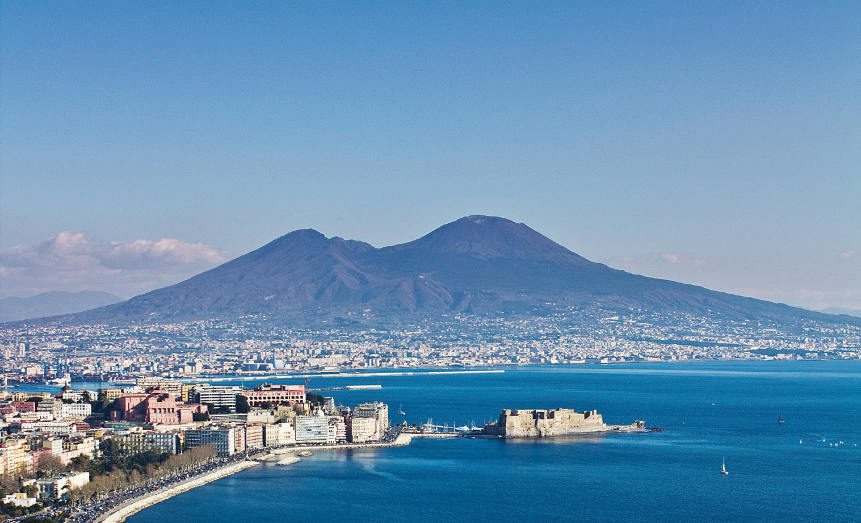
\includegraphics[width=5in]
{vesuvius-bay-of-naples.jpg}
\caption{Mount Vesuvius and Bay of Naples} 
\label{fig-naples}
\end{figure}


\newpage
\tableofcontents
\chapter*{Foreword}
\addcontentsline{toc}{chapter}{Foreword}

Welcome to Bayesuvius! a proto-book uploaded to github.

A different Bayesian network is discussed
 in each chapter. Each chapter title is 
the name of a Bnet. Chapter titles are
 in alphabetical order.

This is a volcano in its early stages.
 First version uploaded to a github repo 
called Bayesuvius on June 24, 2020. 
First version only covers 2 Bnets
(Linear Regression and GAN). 
I will add more chapters periodically.
 Remember, this is a moonlighting effort 
so I can't do it all at once.

For any questions about notation, 
please go to Notational Conventions section.

Requests and advice are welcomed.


\bigskip
\noindent Thanks for reading this

\noindent Robert R. Tucci

\noindent www.ar-tiste.xyz
\bigskip
\\
\noindent{\bf ADDENDA}
\begin{itemize}
\item{\bf August 15, 2021:} At 
this point in time, the book 
has grown to 67 Chapters and 433 pages.
Today, I am self-publishing it as an ebook
at Amazon and similar outlets. It
will still be free.
\end{itemize}


\section{Definition of a Bayesian Network}
\label{ch-bnet-def}

A {\bf directed graph} $G=(V,E)$
consists of two sets, $V$
and $E$. $V$ contains
the {\bf vertices (nodes)}
and $E$ contains the {\bf edges (arrows)}.
An arrow $a\rarrow b$ is an
ordered pair 
$(a,b)$ where $a, b\in V$.
The {\bf parents} 
of a node $x$ are 
those nodes $a$
such that there are arrows 
$a\rarrow x$.
The {\bf children} of a node
$x$
are those nodes $b$
such that there are arrows $x\rarrow b$.
The {\bf neighbors}
of a node $x$
is the set of parents and 
children of $x$.
A {\bf path} is a 
set of nodes that 
are connected 
by arrows, so 
that all nodes
have 1 or 2 neighbors,
but only two nodes ({\bf open path})
or zero nodes ({\bf closed path})
have only one neighbor.
A {\bf directed path}
is a path in
which all the arrows point
in the same direction.
A {\bf loop}
is a closed path;i.e.,
a path in which all
nodes have exactly 2 neighbors.
A {\bf cycle} is a directed loop.
A {\bf Directed Acyclic Graph (DAG)}
is a directed graph that has no
cycles. 


A {\bf fully connected directed graph}
is 
a directed graph
in which 
every node has all other 
nodes as neighbors.
Figs.\ref{fig-full-conn-4-line}
and
\ref{fig-full-conn-4-square}
show 2 different
ways of drawing
the same directed graph,
a fully connected graph with 4 nodes.
Note that a convenient
way
to label
the nodes of a fully
connected directed
graph
with $N$ nodes
is to point
arrows
from 
$\rvx_k$ to $\rvx_j$
where $j=0, 1, 2,\ldots, N-1$
and 
$k=j-1, j-2, \ldots, 0$.


\begin{figure}[h!]
$$
\xymatrix{
\rvx_3
&\rvx_2\ar[l]
&\rvx_1\ar[l]\ar@/_1pc/[ll]
&\rvx_0\ar[l]\ar@/_2pc/[ll]\ar@/_2pc/[lll]
}
$$
\caption{Fully 
connected directed  graph with 4 nodes,
drawn as a line.}
\label{fig-full-conn-4-line}
\end{figure}

\begin{figure}[h!]
$$
\xymatrix{
\rvx_0\ar[r]\ar[d]\ar[rd]&\rvx_1\ar[d]\ar[ld]
\\
\rvx_2\ar[r]&\rvx_3
}
$$
\caption{Fully 
connected directed  graph with 4 nodes,
drawn as a square.}
\label{fig-full-conn-4-square}
\end{figure}

\hrule

A {\bf Bayesian network (bnet)}
consists of a DAG 
and a 
{\bf Transition 
Probability Matrix (TPM)}
associated 
with each node
of the graph.
A TPM is often 
called a {\bf Conditional Probability
Table 
(CPT)}.
The {\bf structure} of a bnet
is its DAG alone, sans the TPMs.


In 
this book,
random  variables are
 indicated by 
underlined letters and their values 
by non-underlined letters.
 Each node of a bnet is
 labelled by a random variable.
 Thus, $\rvx=x$ means that node 
$\rvx$ is in state $x$.


\hrule\noindent
{\bf Some sets of nodes 
associated 
with each node $\rva$
of a bnet}
\begin{itemize}
\item
$ch(\rva)=$ children of $\rva$.
\item
$pa(\rva)=$ parents of $\rva$.
\item
$nb(\rva)=pa(\rva)\cup ch(\rva)=$ 
neighbors of $\rva$.
\item
$de(\rva)=\cup_{n=1}^{\infty}ch^n(\rva)=$
$ch(\rva)\cup ch\circ ch(\rva)\cup\ldots$, 
descendants of $\rva$. 
\item
$an(\rva)=\cup_{n=1}^{\infty}pa^n(\rva)=$
$pa(\rva)\cup pa\circ pa(\rva)\cup\ldots$, 
ancestors of $\rva$.
\end{itemize}
\hrule
In this book,
we will use 
$\rva.$
to indicate
a {\bf multi-node (node set,
node array)} $\rva.=
(\rva_j)_{j=0, 1, \ldots , na-1}$.
We will often
treat multinodes as if
they were sets, and
combine them with
the usual
set
operators.
For instance,
for two
multinodes $\rva.$
and $\rvb.$,
we define
$\rva.\cup\rvb.$,
$\rva.\cap\rvb.$,
$\rva.-\rvb.$
and
$\rva.\subset\rvb.$
in the obvious way.
We 
will indicate
a singleton set (single
node multi-node) $\rva.=\{\rva\}$
simply by $\rva.=\rva$.
For instance,
$\rva.-\rvb=\rva.-\{\rvb\}$.
\hrule

The TPM of a node
$\rvx$ of a bnet
is a matrix of
probabilities 
$P(\rvx=x|pa(\rvx)=a.)$.

A bnet
with nodes $\rvx.$
represents
a probability
distribution

\beq
P(x.)=
\prod_j
P(\rvx_j=x_j|
(\rvx_k=x_k)_{k: \rvx_k\in pa(\rvx_j)})
\;.
\label{eq-chain-rule-bnet}
\eeq

Note that
for a fully connected bnet
with $N$ nodes,
Eq.(\ref{eq-chain-rule-bnet})
becomes

\beq
P(x.)=
\prod_{j=0}^{N-1}
P(x_j| 
(x_k)_{k=j-1, j-2, \ldots, 0})
\;.
\label{eq-chain-rule-cond-probs}
\eeq
For example, if $N=4$,
Eq.(\ref{eq-chain-rule-cond-probs})
 becomes

\beq
P(x_0, x_1,x_2, x_3)=
P(x_3|x_2, x_1, x_0)
P(x_2|x_1, x_0)
P(x_1|x_0)
P(x_0)
\;.
\eeq
We see that 
Eq.(\ref{eq-chain-rule-cond-probs})
is just the chain rule for 
conditional probabilities.








\chapter*{Notational Conventions and Preliminaries}
\addcontentsline{toc}{chapter}{Notational Conventions and Preliminaries}

\label{ch0-conventions}
\section{Some abbreviations frequently
used throughout this book}

\begin{itemize}
\item
bnet= Bnet= Bayesian Network
\item
CPT = Conditional Probabilities Table,
 same as TPM
\item
DAG = Directed Acyclic Graph
\item
i.i.d.= independent identically
distributed.
 \item
 RCT= Randomized Controlled Trial,
a.k.a. A/B testing.

\item
TPM= Transition Probability Matrix,
same as CPT

\end{itemize}

\section{${\cal N}(!a)$}
$\caln(!a)$ will denote
a normalization constant that does not depend
on $a$. For example, $P(x)=\caln(!x)e^{-x}$
where $\int_0^\infty dx \;P(x)=1$.

\section{One hot vector}
A {\bf one hot  vector}
is a vector with all entries
equal to zero with
the exception of a single entry which is one.
A {\bf one cold vector}  is a vector with all entries
equal to one with the exception of  a
single entry which is zero.
For example, if $x^n=(x_0, x_1, \ldots,
x_{n-1})$ and
$x_i=\delta(i,0)$ then $x^n$ is one hot.

Two types of
sets that one frequently encounters
are {\bf categorical sets} (a.k.a. ``nominal sets", i.e.,
sets with ``named" elements, with elements given a ``nomme")
and {\bf numerical sets} (a.k.a. ``ordinal sets", i.e., sets
 with ``ordered"
elements).
For example, $\{1,2,5\}$ is a numerical set
because its elements have a natural order,
and $\{\text{cat, dog, bird}\}$ is a  categorical set
because its elements don't have a natural order.

In Machine Learning (ML),
one often encodes categorical sets as one-hot vectors.
For example, suppose we have 4 binary registers (i.e., nodes)
 $x_3, x_2,x_1, x_0$
and  the categorical set $\{\text{cat, dog, canary}\}$.
Then a possible {\bf one-hot encoding}
of the set
is cat=0001, dog=0010 and canary=0100.
This differs from
a {\bf binary encoding} of the set such as
cat=0000, dog=0001, canary=0011.
Clearly, a binary encoding requires
fewer registers than a one-hot
encoding to
encode the same set,
and the one-hot encoding
of a set with $n$ elements requires
$n$ or more registers.

\section{Special sets}
Define $\ZZ, \RR, \CC$ to be
 the integers, real numbers
 and complex numbers, respectively.

For $a<b$, define $\ZZ_I$
to be the integers in the
interval $I$, where
$I=[a,b],[a,b),(a,b],(a,b)$
(i.e, $I$ can be closed or
 open on either side).

$A_{>0}=\{k\in A: k>0\}$ for $A=\ZZ, \RR$.

\section{Kronecker
delta function}

 For $x,y$ in discrete set $S$,
\beq
\delta(x,y)=\left\{
\begin{array}{l}
1\;{\rm if}\; x=y
\\
0 \;{\rm if}\; x\neq y
\end{array}
\right.
\eeq

\section{Dirac delta function}
 For $x,y\in\RR$,
\beq
\int^{+\infty}_{-\infty}dx\;\delta(x-y)f(x)=f(y)
\eeq

\section{Indicator function
(a.k.a. Truth function)}
\beq
\indi(\cals)=\left\{
\begin{array}{l}
1\;{\rm if\; \cals\; is\; true}
\\
0 \;{\rm if \;\cals\; is \;false}
\end{array}
\right.
\eeq
For example, $\delta(x,y)=\indi(x=y)$.

\section{Majority function}
The {\bf majority function}  is defined as follows.

\beq
\begin{array}{ll}
{\tt majority}(L)=&
\text{ most common element of  list $L$}
\\
&\text{(ties resolved by chance)}
\end{array}
\eeq
Note that the majority function
acts on lists, not sets. By definition,
all elements of a set appear only once in the set.
${\tt majority}(L)$
is usually
used when the elements of
$L$ are categorical (i.e., not real numbers).
When they are real numbers,
it makes more sense to use, instead of
${\tt majority}(L)$, a simple average
of the elements of $L$.


\section{Underlined letters
 indicate random variables}
Random variables will be indicated by
underlined letters and their values
by non-underlined letters.
 Each node of a bnet will be
 labelled by a random variable.
 Thus, $\rvx=x$ means that node
$\rvx$ is in state $x$.

It is more
conventional to
use an upper
case letter to
indicate
a random
variable
and a lower case letter
for its state.
Thus, $X=x$ means that
random variable
$X$ is in state $x$.
However,
we have
opted
in this
book to
avoid
that notation,
because
we often
want to define
certain lower
case letters
to be random variables
or, conversely, define certain upper
case letters to
be non-random variables.

\section{Probability distributions}
 $P_\rvx(x)=P(\rvx=x)=P(x)$ is the probability that random variable $\rvx$ equals $x\in S_\rvx$. $S_\rvx$ is the set of states (i.e., values) that $\rvx$ can assume and $n_\rvx = |S_\rvx|$ is the size (a.k.a. cardinality) of that set. Hence,
\beq
\sum_{x\in S_\rvx}P_\rvx(x)=1
\eeq

\hrule
\beq
P_{\rvx,\rvy}(x,y)=P(\rvx=x, \rvy=y)=P(x,y)
\eeq
\beq
P_{\rvx|\rvy}(x|y)=P(\rvx=x| \rvy=y)=P(x|y)=\frac{P(x,y)}{P(y)}
\eeq



\section{Discretization
of continuous
probability distributions}

The TPM of a node
of a bnet can be either a discrete or
a continuous probability distribution.
To go from continuous to discrete, one
replaces integrals over states of a node
 by sums over new states, and Dirac delta
functions by Kronecker delta functions.
 More precisely, consider a function
$f: [a, b]\rarrow \RR$. Express
 $[a,b]$ as
a union of
small, disjoint (except for
one point) closed sub-intervals (bins) of
length $\Delta x$.
Name one point
in each bin to be the representative of that bin,
and  let $S_\rvx$ be the
set of all the bin representatives. This is called
discretization or binning. Then

\beq
\frac{1}{(b-a)}
\int_{[a,b]} dx \; f(x)\rarrow
\frac{\Delta x}{(b-a)} \sum_{x\in S_\rvx}f(x)
=
\frac{1}{n_\rvx} \sum_{x\in S_\rvx}f(x)
 \;.
\eeq
Both sides of last equation are 1 when $f(x)=1$.
 Furthermore, if $y\in S_\rvx$, then

\beq
\int_{[a,b]} dx \; \delta(x-y)f(x)=f(y)
\rarrow \sum_{x\in S_\rvx}\delta(x,y)f(x)
=f(y)
\;.
\eeq

As usual in this book, let $S_\rvx$ denote the set of
values that the random variable $\rvx$ can take.
When $S_\rvx\subset \RR$,
we will assume that $S_\rvx$
for a probability distribution $P(x)$
can be either a discrete or a continuous
subset of $\RR$.\footnote{By a ``continuous set" we
mean a finite set of intervals
 each of which has non-zero length.}
When $S_\rvx$ is a discrete subset of $\RR$, $P(x)$
will denote a probability distribution
for which $\sum_{x\in S_\rvx}P(x)=1$, whereas when
$S_\rvx$ is continuous, $P(x)$ will denote
a probability density
for which $\int_{x\in S_\rvx}dx\; P(x)=1$.

\section{Samples,
i.i.d. variables}
\beq
\vec{x}= (x[0], x[1], x[2] \ldots,
 x[nsam(\vecx)-1])=x[:]
\eeq

 $nsam(\vecx)$ is the number of samples
 of $\vecx$.
$\rvx[\sigma]\in S_\rvx$ are
 i.i.d. (independent identically distributed)
samples with

 \beq
x[\sigma]\sim P_\rvx\;\;({\rm i.e.}\; P_{\ul{x[\sigma]}}=P_\rvx)
\eeq

\beq
P(\rvx=x)=\frac{1}{nsam(\vecx)}\sum_\sigma \indi(x[\sigma]=x)
\eeq
Hence, for any $f:S_\rvx\rarrow \RR$,
\beq
\sum_x P(\rvx=x)f(x)
=\frac{1}{nsam(\vecx)}\sum_\sigma f(x[\sigma])
\eeq


If we use two sampled variables, say $\vecx$ and $\vecy$,
in a given bnet, their number of samples
$nsam(\vecx)$ and $nsam(\vecy)$ need not be equal.

\hrule
\beq
P(\vecx) = \prod_\sigma P(x[\sigma])
\eeq

\beq
\sum_\vecx = \prod_\sigma\sum_{x[\sigma]}
\eeq

\beq
\partial_\vecx =
[\partial_{x[0]}, \partial_{x[1]},\partial_{x[2]}, \dots, \partial_{x[nsam(\vecx)-1]}]
\eeq

\hrule
\beqa
P(\vecx)&\approx& [\prod_x P(x)^{P(x)}]^{nsam(\vecx)} \\
&=& e^{nsam(\vecx)\sum_x P(x)\ln P(x)}\\
&=& e^{-nsam(\vecx)H(P_\rvx)}
\eeqa

\section{Expected Value and Variance}

Given a random variable
 $\rvx$ with states $S_\rvx$ and
a function $f:S_\rvx\rarrow \RR$, define

\beq
E_\rvx[f(\rvx)]=
E_{x\sim P(x)}[f(x)] = \sum_x P(x) f(x)
\eeq

\beqa
Var_\rvx[f(\rvx)]&=& E_\rvx
\left[(f(\rvx)-E_\rvx[f(\rvx)])^2\right]
\\
&=&
E_\rvx[f(\rvx)^2]-(E_\rvx[f(\rvx)])^2
\eeqa

\beq
E[\rvx]=E_\rvx[\rvx]
\eeq

\beq
Var[\rvx]=
Var_\rvx[\rvx]
\eeq



\section{Conditional Expected Value}

Given a random variable $\rvx$ with states $S_\rvx$, a random variable $\rvy$ with states $S_\rvy,$ and a function $f:S_\rvx\times S_\rvy\rarrow \RR$, define

\beq
E_{\rvx|\rvy}[f(\rvx, \rvy)]=
\sum_x P(x|\rvy) f(x, \rvy)
\;,
\eeq

\beq
E_{\rvx|\rvy=y}[f(\rvx, y)]=
E_{\rvx|y}[f(\rvx, y)]= \sum_x P(x| y) f(x, y)
\;.
\eeq
Note that

\beqa
E_\rvy[E_{\rvx|\rvy}[f(\rvx, \rvy)]]&=&
\sum_{x,y}P(x|y)P(y)f(x,y)
\\&=&
\sum_{x,y}P(x,y)f(x,y)
\\&=&
E_{\rvx, \rvy}[f(\rvx, \rvy)]
\;.
\eeqa



\section{Notation
for covariances}
Consider two random variables $\rvx, \rvy$.

\begin{itemize}
\item
Mean value of $\rvx$
\beq
\av{\rvx}=
E_\rvx[\rvx]
\eeq

\item
Signed distance of $\rvx$ to its mean value
\beq
\Delta \rvx = \rvx - \av{\rvx}
\eeq

\item
Covariance of $(\rvx, \rvy)$
\beq
Cov(\rvx, \rvy)=\av{\rvx, \rvy}=
\av{\Delta \rvx \Delta \rvy}
=
\av{\rvx\rvy}-\av{\rvx}\av{\rvy}
\eeq

$\av{\rvx, \rvy}$ is symmetric
(i.e., $\av{\rvx, \rvy}=\av{\rvy, \rvx}$)
and bilinear (i.e.,
$\av{\sum_i \alp_i\rvx_i, \rvy}
=
\sum_i\alp_i\av{\rvx_i, \rvy}$, where
$\alp_i\in \RR$
are non-random scalars
and $\rvx_i, \rvy\in\RR$ are
real-valued random
variables.)

\item
Variance of $\rvx$
\beq
Var(\rvx)=\av{\rvx, \rvx}
\eeq

\item
Standard deviation or $\rvx$
\beq
\sigma_\rvx=\sqrt{\av{\rvx, \rvx}}
\eeq

\item
Correlation Coefficient of $(\rvx, \rvy)$
\beq
\rho_{\rvx, \rvy}=
\frac{\av{\rvx, \rvy}}
{\sqrt{\av{\rvx, \rvx}\av{\rvy, \rvy}}}
\eeq
\end{itemize}

\section{Conditional Covariance}
Let $\rvx, \rvy, \rva$
be random variables.
The covariance $Cov(\rvx, \rvy|\rva)$
of $\rvx$ and $\rvy$
given $\rva$, is defined
the same
way as $Cov(\rvx, \rvy)$,
except that all
expected values are
conditioned on $\rva$.



\beq
Cov(\rvx, \rvy|\rva)=
\av{\rvx, \rvy}_{|\rva}
=
\av{(\rvx-\av{\rvx}_{|\rva})
(\rvy-\av{\rvy}_{|\rva})}_{|\rva}
\eeq
where

\beq
\av{\rvx}_{|\rva}=E_{\rvx|\rva}[\rvx]
\;.
\eeq

\section{Law of Total Variance}

\begin{claim}
Suppose $P:S_\rvx\times S_\rvy\rarrow [0,1]$
is a probability distribution.
Suppose $f:S_\rvx\times S_\rvy\rarrow \RR$
 and $f=f(x,y)$. Then
\beq
Var_{\rvx, \rvy}(f)=
E_\rvy[Var_{\rvx|\rvy}(f)]
+
Var_\rvy(E_{\rvx|\rvy}[f])
\;.
\eeq
In particular,
\beq
Var_{\rvx}(x)=
E_\rvy[Var_{\rvx|\rvy}(x)]
+
Var_\rvy(E_{\rvx|\rvy}[x])
\;.
\eeq

\end{claim}
\proof

Let
\beq
A=\sum_y P(y)\left(\sum_x P(x|y)f\right)^2
\;.
\eeq
Then

\beqa
Var_{\rvx, \rvy}(f)&=& \sum_{x,y}P(x,y)f^2 -
\left( \sum_{x,y} P(x,y) f\right)^2
\\
&=&
\left\{
\begin{array}{l}
\sum_{x,y}P(x,y)f^2
-A
\\
+\left(A-\left( \sum_{x,y} P(x,y) f\right)^2\right)
\end{array}
\right.
\eeqa

\beqa
E_\rvy[Var_{\rvx|\rvy}(f)]
&=&
\sum_y P(y)\left(\sum_x P(x|y)f^2
-
\left(\sum_x P(x|y)f\right)^2
\right)
\\
&=&
\sum_{x,y}P(x,y)f^2
-A
\eeqa

\beqa
Var_\rvy(E_{\rvx|\rvy}[f])
&=&
\sum_y P(y)
\left(\sum_x P(x|y)f\right)^2
-\left(
\sum_y P(y)\sum_xP(x|y)f
\right)^2
\\
&=&
A-\left( \sum_{x,y} P(x,y) f\right)^2
\eeqa
\qed





\section{Normal Distribution}


For $x, \mu, \sigma\in \RR$,
$\sigma >0$, we define the Normal Distribution
(see Fig.\ref{fig-norm-dist}) by

\beq
\caln(x; \mu, \sigma^2)=
\frac{1}{\sigma\sqrt{2\pi}}
e^{-\;\frac{1}{2}\left(
\frac{x-\mu}{\sigma}\right)^2}
\;.
\eeq

For a {\bf standard deviation}
$\s$, the {\bf precision} $\tau$
is defined as $\tau=\frac{1}{\s^2}$.

\begin{claim}
If

\beq
\rvx_1\sim \caln(\mu_1, \s^2_1)
\eeq
and

\beq
\rvx_2\sim \caln( \mu_2, \s^2_2)
\eeq
then
\beq
\rvx=\rvx_1 +\rvx_2 \sim \caln(\mu_1 + \mu_2, \s^2_1 + \s^2_2)
\;.
\eeq
\end{claim}
\proof

\beqa
P(\rvx=x)&=&\caln(!x)
\int_{-\infty}^{+\infty}dx_2\;
P(\rvx_1 + \rvx_2 = x|\rvx_2=x_2)P(x_2)
\\
&=&\caln(!x)
\int_{-\infty}^{+\infty}dx_2\;
\caln(x-x_2;\mu_1, \s^2_1)
\caln(x_2;\mu_2, \s^2_2)
\\
&=&
\caln(x;\mu_1 +\mu_2; \s^2_1+\s^2_2)
\eeqa
\qed

\begin{figure}[h!]
\centering
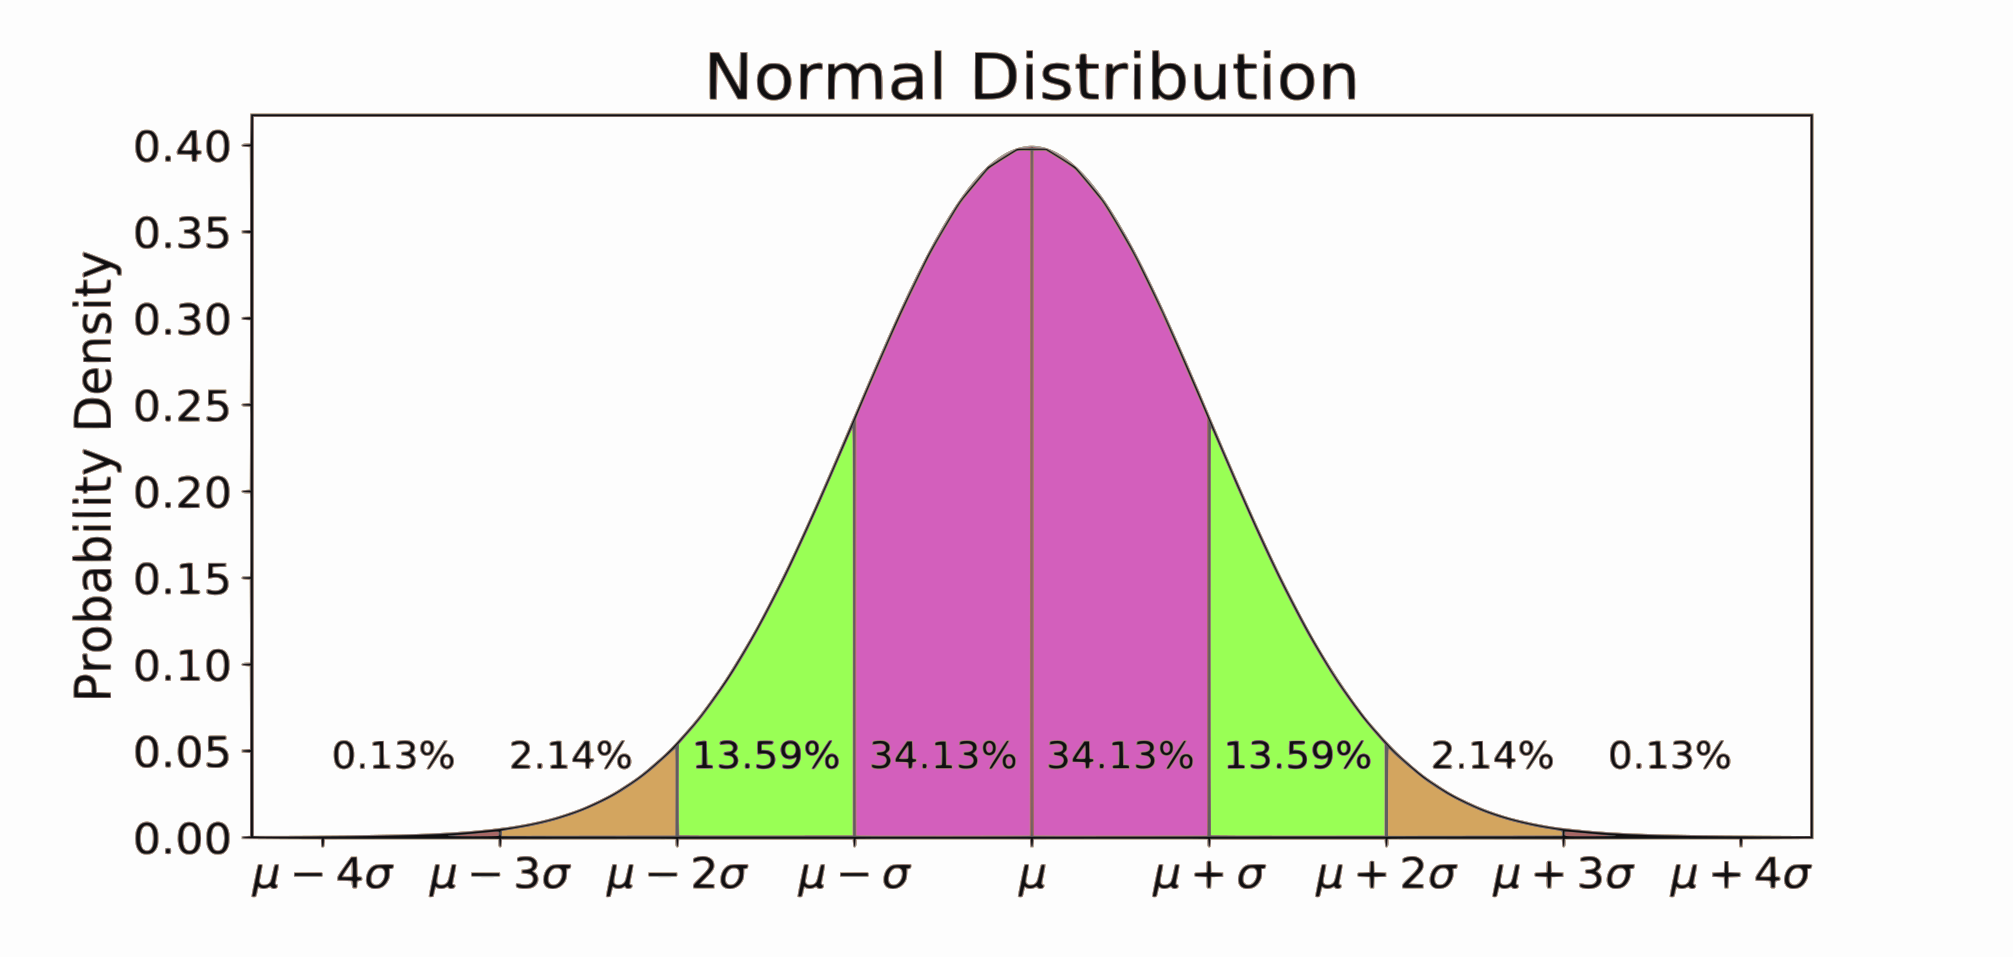
\includegraphics[width=5in]
{conventions/normal-dist.png}
\caption{Normal Distribution
$\caln(x;\mu, \s^2)$.}
\label{fig-norm-dist}
\end{figure}

The {\bf Standard Normal Distribution} $P_{SND}(x)$
and its cumulative distribution $\Phi(x)$ are defined by

\beq
P_{SND}(x)=\caln(x; \mu=0, \s=1)
\eeq

\beq
\Phi(x) = \int_{-\infty}^x dx'\;P_{SND}(x')
\eeq

The {\bf error function} ${\rm erf}:\RR\rarrow [-1,1]$
is defined by
\beq
{\rm erf}(x) = \frac{2}{\sqrt{\pi}}
\int_0^x du \; e^{-\;\frac{u^2}{2}}
\eeq

Note that

\beq
\Phi(x)= \frac{1}{2} + \frac{1}{2}{\rm erf}(x)
\label{eq-Phi-erf}
\eeq
Eq.(\ref{eq-Phi-erf})
is interpreted geometrically in Fig.\ref{fig-erf}.

\begin{figure}[h!]
\centering
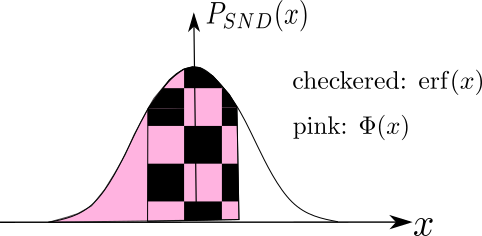
\includegraphics[width=2.8in]
{conventions/erf.png}
\caption{Plot of Standard
Normal Distribution $P_{SND}(x)$.
 Values of ${\rm erf}(x)$ and $\Phi(x)$
 equal indicated areas.}
 \label{fig-erf}
\end{figure}
\section{Uniform Distribution}
For $a<b$, $x\in [a,b]$

\beq
\calu(x;a,b) =
\frac{1}{b-a}
\eeq

\section {Softmax function
(a.k.a. Boltzmann Distribution)}

The Softmax function
 is defined by
\beq
P(x_i
|x.)=\frac{e^{x_i}}{\sum_i e^{x_i}}=
\softmax(x.)_i
\label{eq-softmax}
\eeq
The
Boltzmann distribution is defined as

\beq
P(\rvE_a=E_a)=\frac{\exp(-\;\frac{E_a}{kT})}{\sum_{a}
\exp(-\;\frac{E_{a}}{kT})}=
P(\frac{-E_a}{kT}|E.)\eeq
for a system with energies $E_a$
and temperature $T$,
where $k$
is Boltzmann's constant.

The function
softmax() is called softmax because if we
approximate the exponentials,
 both in the numerator and denominator
of Eq.(\ref{eq-softmax}),
by the largest one
of them or zero,
we get

\beq
\softmax(x.)_i\approx \indi(i=\argmax_k x_k)
\;.
\eeq
Thus, softmax($x.$)
returns a continuous
function that approximates a one-hot vector
that is 1 at the
$i$th
component, where
$i=\argmax_k(x_k)$,
and zero at the other components.

Note that
\beq
\pder{\ln P(x_i|x)}{x_a}
=
\pder{}{x_a}\ln\left[
\frac{e^{x_i}}{\sum_i e^{x_i}}
\right]
=
\delta(a,i)
-
P(x_a|x)
\eeq

For 2 variables $x_0, x_1$,
\beqa
P(x_0|x.)&=&
\frac{e^{x_0}}{e^{x_0} + e^{x_1}}\\
&=&\smoid(x_0-x_1)
\;,
\eeqa

\beq
P(x_1|x.)=\smoid(x_1-x_0)
\;.
\eeq

\section{Sigmoid and log-odds functions}
\label{sec0-smoid}
The {\bf sigmoid (a.k.a. exp-it,  logistic) function} smoid:$\RR\rarrow [0,1]$
is defined by
\beq
\smoid(x)=
\frac{1}{1+e^{-x}}
\eeq
$\smoid()$ is monotonically
increasing with $\smoid(-\infty)=0$,
$\smoid(0)=1/2$
and $\smoid(+\infty)=1$.
Note that for $x<<0$, $\smoid(x)\approx e^x$, which
is why ``smoid" is also called ``expit".

\beqa
\smoid(x)+\smoid(-x)&=&
\frac{1}{1+e^{-x}}+\frac{1}{1+e^x}\\
&=&\frac{2+e^x+e^{-x}}{2+e^x+e^{-x}}
\\&=&1
\eeqa


The {\bf log-odds (a.k.a. log-it) function}
lodds:$[0,1]\rarrow \RR$ is defined by

\beq
{\rm lodds}(p)=\ln\frac{p}{1-p}
\eeq
Note that for $0< p<<1$, $\lodds(x)\approx \ln p$,
which is why ``lodds" is also called ``logit".

Note that for $x<<1$, $\smoid(x)\approx e^x<<1$,
so $\lodds(e^x)\approx \ln(e^x)=x$.
More generally, it
is easy to check that for any $p\in[0,1]$ and $x\in \RR$,
\beq
\lodds[\smoid(x)]=x
\eeq

\beq
\smoid [\lodds(p)] =p
\eeq
Hence,
$\lodds()$ is the inverse of $\smoid()$ and vice-versa.

\begin{claim}
\beq
\smoid'(x)=\smoid(x)[1-\smoid(x)]
\eeq

\beq
\smoid''(x)=\smoid'(x)[1-2\smoid(x)]
\eeq
\end{claim}
\proof

In this proof, we will
abbreviate $\smoid(x)$ by $s(x)$.
\beq
1-s(x)=1 -\;\frac{1}{1+e^{-x}}=
\frac{e^{-x}}{1+e^{-x}}
\eeq

\beq
s'(x)= \frac{e^{-x}}{(1+e^{-x})^2}
=s(x)[1-s(x)]
\eeq

\beqa
s''(x)&=&s'(x)[1-s(x)]
+
s(x)(-1)s'(x)
\\
&=&
s'(x)[1-2s(x)]
\\
&=&
s(x)[1-s(x)][1-2s(x)]
\eeqa
\qed

\section{Estimand, Estimator (curve-fit, cfit), Estimate, Bias}
\label{sec0-estimand}
For an {\bf estimand} $\theta$,
an {\bf estimator (a.k.a. curve fit,
cfit)} $\ul{\HAT{\theta}}$
gives {\bf estimate} $E[\ul{\HAT{\theta}}(\theta)]=\theta+b$
with {\bf bias} $b$.
We say this estimate is an {\bf unbiased estimate}
if $b=0$.

Note that, strictly
speaking, an estimator is a function
waiting to be averaged over
and denoted by a letter with a hat,
whereas an estimate is a real number
denoted by a letter without a hat.
Unfortunately, the
words ``estimator" and
``estimate" are often used interchangeably,
as if they were synonyms.
And often the estimate $\theta + b$
is denoted by a letter with a hat too.
In some sense, an estimator is an estimate
of a curve, so it's understandable that
the terms ``estimator" and ``estimate"
are used synonymously.
In this book, we will bow to traditional
practice and
also use
the terms ``estimator" and ``estimate"
synonymously, and use a letter
with a hat to denote either of them.
This is not
ambiguous as long as we don't
use the same letter with a
hat to denote two different quantities, of course.
When we need to distinguish semantically
between the real value and the function,
we will call the function a cfit,
and the real value the estimate.

\section{Maximum Likelihood Estimate,
Likelihood Ratio Test}
\label{sec0-likelihood-ratio}

Given a bnet, let $P(x|\theta)$
be its full joint probability distribution,
where
$x$ denotes the joint state
of all the nodes and $\theta$
denotes all the parameters.
 $P(x|\theta)$ is often
called the {\bf likelihood function of $\theta$}
and is denoted by

\beq
L(\theta)= P(x|\theta)
\eeq
It's called a likehood of $\theta$
because, even though it's a probability,
it isn't the probability of $\theta$,
but rather of $x$.

The value of $\theta$
that we obtain by maximizing $L(\theta)$
over $\theta$ is called
the
{\bf maximum likelihood
estimate (MLE) of $\theta$}. Let us denote it by
$\HAT{\theta}$. Note that\footnote{``sup" stands for supremum.
It's a generalization of the function $\max()$
to arbitrary sets
that might not be discrete or finite.
If $S$ is a
finite set,
then $\sup_{\theta\in S} f(\theta)=
\max_{\theta\in S} f(\theta)$
for any function $f:S\rarrow \RR$.
Likewise, ``inf" stands for infimum,
and it generalizes the $\min()$ function.}

\beq
\sup_{\theta\in S}L(\theta)=
L(\HAT{\theta})
\eeq


Let $S_0, S_1$ be disjoint sets such that
 $S=S_0\cup S_1$.
We'll say
the {\bf null hypothesis $H_0$} holds
 if $\theta\in S_0$,
and the {\bf alternative hypothesis $H_1$}
holds if
$\theta\in S_1$.
The {\bf likelihood ratio (LR) test statistic}
is defined by


\beq
R=-2\ln
\left(\frac{\sup_{\theta\in S_0}L(\theta)}
{\sup_{\theta\in S}L(\theta)}\right)
\eeq
$R\geq 0$ and $R=0$ if  $S_0=S$.
For some small $c>0$,
if $R<c$, then we reject the alternative hypothesis,
and if $R>c$, we accept it.




If $S_0=\{\theta_0\}$,
then

\beq
R= -2[\ln L(\theta_0) -\ln L(\HAT{\theta})]
\eeq


\section{Mean Square Error (MSE)}

Suppose we are
given $nsam$ samples $y^\s\in\RR$
labeled by an index $\s$,
and a cfit $\haty^\s(a)\in\RR$
that depends on a parameter $a\in\RR$.
Define the {\bf Mean Square
Error (MSE)}
by

\beq
MSE(a) = \frac{1}{nsam}\sum_\s (y^\s-\haty^\s(a))^2
\;.
\eeq
For example, in Linear Regression (LR),
we have $\haty^\s= a_0 + a_1 x^\s$
where $a=(a_0, a_1)$ is a deterministic
parameter.
If the samples $y^\s$
are i.i.d,
then we can also write


\beq
MSE(a)=E_{|a}[(\rvy-\ul{\haty}(a))^2]
\;.
\eeq
and for LR, $\ul{\haty}(a)=a_0+a_1\rvx$.

Define the {\bf residual} $\Delta\rvy$ by:


\beq
\Delta\rvy(a) =\rvy-\ul{\haty}(a)
\;\;\;\text{ (Hence
$\rvy=\ul{\haty} + \Delta\rvy$)}
\eeq

In the rest of this section,
we will discuss the case that
$\haty^\s(a)$ is independent of $x^\s$.
I call
this the {\bf deterministic MSE (D-MSE)}
model.
Note that this
is different from the LR
case where
$\haty^\s(a)$ does depend on $x^\s$.
In LR, we are trying
to fit
a line to a cigar-shaped
2-D scatter plot.
Here, we are just trying
to estimate
the mean value (center of mass)
of a scatter plot.


\begin{claim}
MSE is minimized
over all functions $\haty$ if
\beq
\haty =E_{|a}[\rvy]
\eeq
\end{claim}
\proof

\beq
MSE = E_{|a}[\rvy^2]-2\haty E_{|a}[\rvy]+ \haty^2
\eeq

\beq
0=\frac{d}{d\haty} MSE = 2(-E_{|a}[\rvy]+\haty)
\eeq
Hence,
\beq
\haty =E_{|a}[\rvy]
\eeq
\qed

Sometimes, we will
use the notation
\beq
\haty_{MSE} = E_{|a=a_{MSE}}[\rvy]
\;.
\eeq

\begin{claim}
Suppose $f(a)$
is a function of $a$.
If $\haty=E_{|a}[\rvy]$, then

\beq
E_{|a}[\Delta \rvy]=
E[\Delta \rvy]=0
\eeq



\beq
E_{|a}
\left[\Delta \rvy f(\rva)\right]=
E
\left[\Delta \rvy f(\rva)\right]=0
\eeq
\end{claim}
\proof

\beq
E_{|a}[\Delta\rvy]=
E_{|a}
\left[\rvy-E_{|a}[\rvy]\right]=
E_{|a}[\rvy]-E_{|a}[\rvy]=0
\eeq

\beq
E[\Delta \rvy] =
 E_{\rva}[E_{|\rva}[\Delta\rvy]]=0
\eeq


\beqa
E_{|\rva}
\left[\Delta \rvy f(\rva)\right]
&=&
f(\rva)
\underbrace{E_{|\rva}
[\Delta\rvy]}_{=0}
\eeqa

\beq
E[\Delta \rvy f(\rva)]
=E_\rva[E_{|\rva}[\Delta\rvy f(\rva)]]=0
\eeq
\qed


\begin{claim}
If $\haty=E_{|a}[\rvy]$, then

\beq
\av{\Delta\rvy, \haty}_{|a}
=0
\label{eq-mse-uncorr}
\eeq

\beq
Var_{|a}[\rvy]
=
Var_{|a}[\haty]
+
Var_{|a}[\Delta\rvy]
\eeq
The same results hold
without the conditioning on $a$.
\end{claim}
\proof

\beqa
\av{\Delta\rvy, \ul{\haty}}_{|a}
&=&
\underbrace{E_{|a}[\Delta\rvy \;\underbrace{\ul{\haty}}
_{f(\rva)}]
}_{=0}
-
\underbrace{E_{|a}[\Delta\rvy]}_{=0}
E_{|a}[ \ul{\haty}]
\eeqa

\beqa
Var_{|a}[\rvy]
&=&
\av{\haty +\Delta\rvy, \haty +\Delta\rvy}_{|a}
\\
&=&
\av{\haty, \haty}_{|a}
+
\av{\Delta\rvy, \Delta\rvy}_{|a}
\;\text{(by Eq.(\ref{eq-mse-uncorr}))}
\\
&=&
Var_{|a}[\haty]
+
Var_{|a}[\Delta\rvy]
\eeqa
The same proof
holds
if we remove all the $|a$
subscripts.
\qed

Fig.\ref{fig-ms-error}
illustrates how
$\rvy=\ul{\haty} +\Delta \rvy$
and the variances of these
quantities add.


\begin{figure}[h!]
\centering
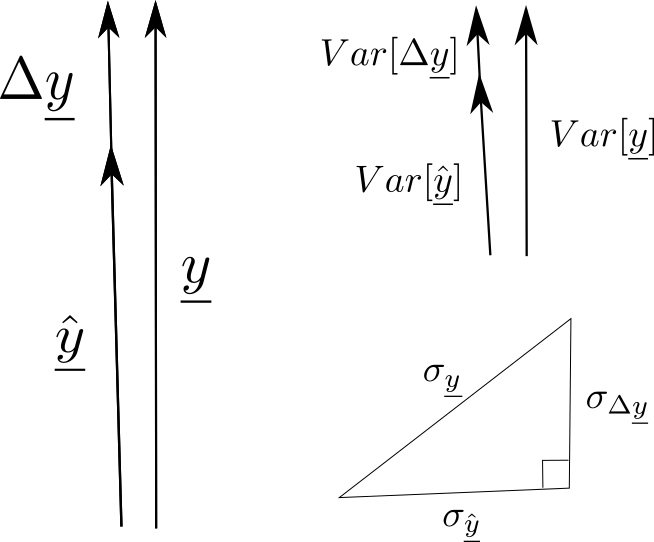
\includegraphics[width=2.3in]
{conventions/ms-error.png}
\caption{$\rvy=\HAT{y}+\Delta y$
and the variances (not standard deviations)
of these quantities add. }
\label{fig-ms-error}
\end{figure}

\section{Cramer-Rao Bound}

This discussion of the Cramer-Rao (CR) bound
is based on Ref.\cite{wiki-cramer-rao}.

Suppose $\rvx$ is a random variable with values $x\in S_\rvx$
and $\theta\in\RR$ is a parameter.
For any function
$f_{\rvx,\theta}: S_\rvx\times \RR\rarrow \RR$,
define

\beq
\av{f_{\rvx,\theta}} =\sum_x P(x|\theta)f_{x,\theta}
\eeq

\beq
\Delta f_{\rvx,\theta}=f_{\rvx,\theta}-\av{f_{\rvx,\theta}}
\eeq

\beq
\av{f_{\rvx,\theta},f_{\rvx,\theta}}=
\av{\Delta f_{\rvx,\theta}\;\Delta f_{\rvx,\theta}}
\eeq

Define the {\bf log likelihood function} by
\beq
LL_\theta = \ln P(x|\theta)
\eeq

Define the {\bf Fisher information} by
\beq
I_\theta=\av{\partial_\theta LL_\theta,\partial_\theta LL_\theta}
\eeq

Note that $LL_\theta\leq 0$.
Let $\theta^*$ be the
value of $\theta$ that maximizes $LL_\theta$.


Note that $I_\theta\geq 0$ and
$I_\theta=0$ when $\theta=\theta^*$
because $\partial_\theta LL_\theta|_{\theta=\theta^*}=0$.
This suggests that $I_\theta$
measures the distance
between $\theta$ and $\theta^*$.



Note that
\beqa
\av{\partial_\theta LL_\theta}&=&
\sum_x P(x|\theta)\frac{1}{P(x|\theta)}
\partial_\theta P(x|\theta)
\\
&=&
\partial_\theta \sum_x P(x|\theta)
\\
&=&
0
\eeqa
Therefore

\beqa
I_\theta &=&\av{[\partial_\theta LL_\theta]^2}
-
\av{\partial_\theta LL_\theta}^2
\\
&=&
\av{[\partial_\theta LL_\theta]^2}
\eeqa

\begin{claim}
\beq
I_\theta = -\av{\partial_\theta^2 LL_\theta}
\eeq
\end{claim}
\proof

\beqa
I_\theta &=& \av{[\partial_\theta LL_\theta]^2}
\\
&=&
\sum_x P(x|\theta)
\frac{1}{P(x|\theta)}
\partial_\theta P(x|\theta)
\partial_\theta \ln P(x|\theta)
\\
&=&
-\sum_x P(x|\theta)\partial_\theta^2 \ln P(x|\theta)
+ \partial_\theta\sum_x
P(x|\theta)\partial_\theta \ln P(x|\theta)
\\
&=&
-\av{\partial_\theta^2 LL_\theta}
+ \partial_\theta^2\sum_x P(x|\theta)
\\
&=&
-\av{\partial_\theta^2 LL_\theta}
\eeqa
\qed

\begin{claim}
If $x=[x_i]_{i=1,2, \ldots \nu}\in \RR^\nu$ are i.i.d., then


\beq
I_\theta = \nu \av{[\partial_\theta LL_{\theta, i}]^2}
\eeq
where

\beq
LL_{\theta, i} = \ln P(x_i|\theta)
\eeq
\end{claim}
\proof

\beqa
LL_\theta
&=& \ln \prod_i P(x_i|\theta)
\\
&=&
\sum_i LL_{\theta, i}
\eeqa

\beqa
I_\theta &=&
\sum_i \sum_j \av{
\partial_\theta LL_{\theta,i}
\partial_\theta LL_{\theta,j}
}
\\
&=&
\sum_i  \av{
[\partial_\theta LL_{\theta,i}]^2}
\\
&=&
\nu \av{
[\partial_\theta LL_{\theta,i}]^2
}
\eeqa
\qed




A function  $t_\rvx:S_\rvx\rarrow \RR$
is called a {\bf test statistic} of random variable $\rvx$.

\begin{claim}(Cramer-Rao bound for single parameter $\theta\in\RR$)

\beq
\av{t_\rvx,t_\rvx}I_\theta \geq
 \left[\partial_\theta\av{t_\rvx}\right]^2
 \label{eq-crao-tx}
 \eeq
\end{claim}
\proof

Cauchy-Schwartz inequality

For two vectors $\veca,\vecb\in\RR^n$:
\beq
\veca\cdot\vecb =|\veca||\vecb|\cos \phi \leq |\veca||\vecb|
\eeq

For two real valued random variables $\rva, \rvb$:
\beq
\av{\rva, \rva} \av{\rvb,\rvb}\geq |\av{\rva,\rvb}|^2
\eeq
Replace

\beq
\rva\rarrow t_\rvx,
\quad\rvb\rarrow \partial_\theta LL_\theta
\eeq
Then

\beqa
\av{t_\rvx, \partial_\theta LL_\theta}
&=&
\av{t_\rvx \partial_\theta LL_\theta}
-
\av{t_\rvx} \underbrace{\av{\partial_\theta LL_\theta}}_{=0}
\\
&=&
\sum_x P(x|\theta)
t_\rvx \frac{1}{P(x|\theta)}\partial_\theta P(x|\theta)
\\
&=&
\partial_\theta\sum_x  t_\rvx P(x|\theta)
\\
&=&
\partial_\theta\av{ t_\rvx}
\eeqa
\qed

See Fig.\ref{fig-cramer-rao}
for a pictorial representation
of Eq.(\ref{eq-crao-tx}).

\begin{figure}[h!]
\centering
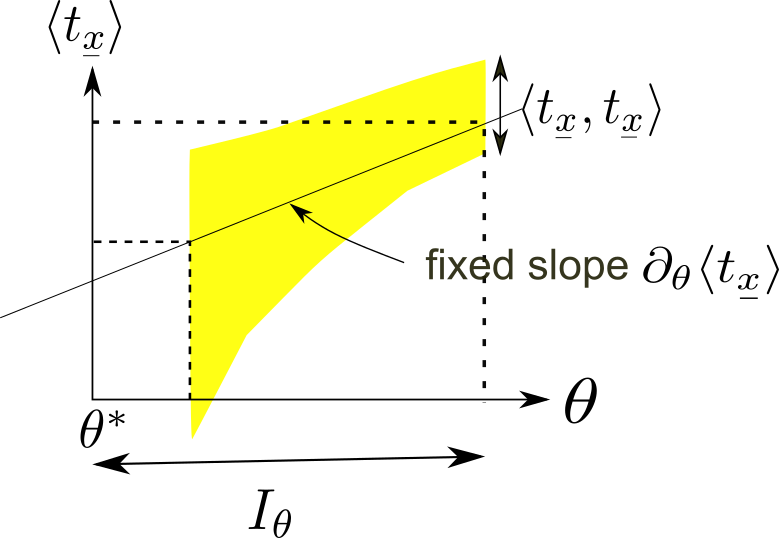
\includegraphics[width=2.7in]
{conventions/cramer-rao.png}
\caption{
In this drawing,
$\theta^*$ is the
value of $\theta$ that maximizes $LL_\theta$.
According
to the CR bound,
the product of the
variance $\av{t_\rvx, t_\rvx}$ and
the distance $I_\theta$
must be greater or equal to $[\partial_\theta\av{t_\rvx}]^2$.
At fixed $[\partial_\theta\av{t_\rvx}]^2$,
if the variance increases, the distance decreases,
and vice versa.
}
\label{fig-cramer-rao}
\end{figure}


Now suppose the test statistic $t_\rvx$
equals an {\bf estimator} $\HAT{\theta}$
of $\theta$ with bias $b_\rvx:S_\rvx \rarrow \RR$.

\beq
t_\rvx = \HAT{\theta}(\rvx) = \theta + b_\rvx
\eeq
$\HAT{\theta}$ is said to be a {\bf biased estimator}
if $b_\rvx\neq 0$ and an {\bf unbiased estimator} if $b_\rvx=0$.

\begin{claim}

\beq
\av{\HAT{\theta}} = \theta + \av{b_\rvx}
\eeq

\beq
\av{\HAT{\theta}, \HAT{\theta}} \geq
\frac{[1 + \partial_\theta\av{b_\rvx}]^2}
{I_\theta}
\label{eq-crao-theta}
\eeq

\beq
\av{[\HAT{\theta}-\theta]^2} \geq
\frac{[1 + \partial_\theta\av{b_\rvx}]^2}
{I_\theta}
+
\av{b_\rvx}^2
\eeq

\end{claim}
\proof
\beqa
\partial_\theta\av{t_\rvx}
&=&
\partial_\theta\av{\theta + b_\rvx}
\\
&=&
\partial_\theta\left[\theta +\av{b_\rvx}\right]
\\
&=&
1 + \partial_\theta\av{b_\rvx}
\eeqa
Eq.(\ref{eq-crao-theta})
follows from Eq.(\ref{eq-crao-tx})
once we replace $t_\rvx$ by $\HAT{\theta}$.

Let
\beq
\Delta \HAT{\theta} =
\HAT{\theta} -\av{\HAT{\theta}}
=
\underbrace{(\HAT{\theta} -\theta)}_\xi  - \av{b_\rvx}
\eeq
Then

\beq
0=\av{\Delta \HAT{\theta}} = \av{\xi} - \av{b_\rvx}
\eeq

\beqa
\frac{[1 + \partial_\theta\av{b_\rvx}]^2}
{I_\theta} &\leq&
\av{[\Delta \HAT{\theta}]^2}
\\
&=&
\av{\xi^2 -2\xi\av{b_\rvx} + \av{b_\rvx}^2}
\\
&=&
\av{\xi^2} -\av{b_\rvx}^2
\eeqa

\qed

Multi-dimensional case:
parameter
 $\theta=[\theta_1, \theta_2, \ldots, \theta_n]^T\in \RR^n$
 and test statistic
 $t_\rvx=[t_{\rvx,1}, t_{\rvx,2}, \ldots, t_{\rvx,n}]^T\in \RR^n$
are column vectors.

Define {\bf Fisher information matrix} by

\beq
[I_\theta]_{i,j}=
\av{\partial_{\theta_i} LL_\theta, \partial_{\theta_j}LL_\theta}
=
\av{\partial_{\theta_i} LL_\theta\;\partial_{\theta_j}LL_\theta}
\eeq

CR bound for multi-dimensional parameter $\theta\in\RR^n$:
\beq
\text{matrix}\left[\av{t_{\rvx,i}, t_{\rvx,j}}\right]\geq
\text{matrix}\left[
\partial_{\theta_i} \av{t_{\rvx,a}}
[I_\theta]^{-1}_{a,b}
\partial_{\theta_j} \av{t_{\rvx,b}}
\right]
\eeq
where we are using the Einstein summation
convention (repeated indices are summed over).
For two matrices $A,B\in\RR^n$, $A\geq B$ means $A-B$ has
non-negative eigenvalues.


\section{Bayes Rule,
Bayesian Updating And Conjugate Priors}

Bayes Rule says:

\beq
P(\theta|x)P(x)
=
P(x|\theta)P(\theta)
\eeq
Expressed diagramatically\footnote{Two bnets are equated if their full probability
distributions (i.e.,
their full instantiations) are equal numerically.
For example,  
$$
\rva\rarrow\rvb\rarrow \rvc = P(c|b)P(b|a)P(a)= \rva\larrow\rvb\larrow\rvc
$$},
we have for  $\rvx\in\RR$:
\beq
\xymatrix{
\rvtheta&\rvx\ar[l]
}
\quad =\quad
\xymatrix{
 \rvtheta\ar[r]&\rvx
}
\eeq
and for $\rvx=(\rvx_1, \rvx_2)\in \RR^2$:
\beq
\begin{array}{c}
\xymatrix@R=.3pc{
&\rvx_1\ar[ld]\ar[dd]
\\
\rvtheta
\\
&\rvx_2\ar[lu]
}
\xymatrix@R=.3pc{\\\quad =\quad}
\xymatrix@R=.3pc{
&\rvx_1\ar[dd]
\\
\rvtheta\ar[ru]\ar[rd]
\\
&\rvx_2
}
\end{array}
\eeq
Note how Bayes rule
allows us to reverse the
direction of the arrows
impinging on $\theta$.
We see from Bayes Rule
that even though
the directions of
the arrows in a
bnet can have causal
motivation, a bnet
with arrows reversed
from their causally
motivated directions
can still be very useful
as a calculation tool.

Another way of stating
Bayes Rule is




\beq
\underbrace{P(\theta|x)}_{\rm posterior}=
\caln(!\theta)
\underbrace{P(x|\theta)}_{\rm likelihood}
\underbrace{P(\theta)}_{\rm prior}
\;.
\eeq

If, for a given likelihood,
the prior and posterior
distributions belong to
the same family (for instance,
they are both
Beta distributions),
then we say that the prior is the
{\bf conjugate prior}
of that likelihood.

For example,
Beta $\sim$ Bernoulli*Beta.
Hence, the
Beta distribution\footnote{See
Ref.\cite{wiki-beta-dist} for a discussion
of the Beta distribution.}
is the conjugate prior of the
Bernoulli distribution\footnote{See
Ref.\cite{wiki-bern-dist} for a discussion
of the Bernoulli distribution}.
More explicitly,
if

\beq
p_1\sim {\rm Beta}(p_1;\alp, \beta)
\eeq
and

\beq
x|p_1\sim {\rm Bernoulli}(x;p_1)
\;,
\eeq
where $p_1=P(x=1)$,
then

\beq
p_1|x\sim {\rm Beta}(p_1;\alp', \beta')
\eeq
where

\beq
\alp'= \alp + x
\eeq

\beq
\beta'= \beta + (1-x)
\eeq


Ref.\cite{wiki-conj-prior}
has a table of
conjugate priors.

Conjugate priors facilitate
Bayesian updating
of the prior to
posterior in a
feedback loop(see Fig.\ref{fig-conj-prior}).

\begin{figure}[h!]
$$\xymatrix{
&x_t\ar[d]
\\
&\stackrel{Bernoulli}{P(x_t|\theta)}\ar@/_2pc/[ld]
\\
\stackrel{Beta}{P(\theta|x_{\leq t})}\ar@/_2pc/[rd]
&&\stackrel{Beta}{P(\theta|x_{\leq t-1})}\ar@/_2pc/[ul]
\\
&t\rarrow t+1 \text{ for } t=0, 1, 2,\ldots
\ar@/_2pc/[ur]
}$$
\caption{Bayesian updating facilitated
by conjugate prior. In this figure,
$x_{\leq t}=(x_0, x_1, \ldots, x_{t-1}, x_t)$.}
\label{fig-conj-prior}
\end{figure}


\section{Linear regression, Ordinary Least Squares (OLS)}
\label{sec0-conv-lr}
Wikipedia articles
\begin{enumerate}
\item
Linear Regression (LR)
\begin{itemize}
\item
linear regression, Ref.\cite{wiki-lr}
\item
 simple linear regression, Ref.\cite{wiki-slr}
\item
errors in variable, Ref.\cite{wiki-errors-in-iv}

\end{itemize}
\item
Least squares (LS)
\begin{itemize}
\item
least squares, Ref.\cite{wiki-lsquares}
\item
ordinary least squares (OLS), Ref.\cite{wiki-ols}
\end{itemize}
\end{enumerate}


Some nomenclature: In LR, the
data consists of
{\bf independent x-variables} $x^\s_1,
 x^\s_2, \ldots x^\s_n$
and a {\bf dependent y-variable} $y^\s$.
We find a linear fit $\haty^\s =
\beta_0 + \sum_{i=1}^n \beta_i x^\s_i$
to the data.
$\haty^\s$ is called the {\bf estimate}
of $y^\s$.
 The coefficients $\beta_0, \beta_i$
are called {\bf regression coefficients}.
$y^\s-\haty^\s=\eps^\s$
are called  the {\bf residuals}.
$\cale =\sum_\s (\eps^\s)^2$
is called the {\bf error or cost}. We choose the
regression coefficients
so as to minimize the error.

Below, we consider two types of LR:

\begin{enumerate}
\item
LR
in which the independent x-variables are non-random.
\item
LR
in which the independent x-variables are random
and i.i.d.
\end{enumerate}

The  term OLS
is often used to refer to LR
of type 1.



For LR of type 2,
there is randomness in $y$
coming from the randomness in $x$
and in the residuals.
For LR of type 1,
there  is randomness in $y$
too, but
it comes
from the residuals
only.

Once one assumes that certain
variables are random, a
``model" (i.e., a bnet,
with probabilities expressed as TPMs)
 must be
specified.


\subsection{LR, assuming
$x_\s$ are non-random}

Let

$\s\in\{0, 1, 2, \ldots, nsam-1\}$ : sample index

$i_0\in\{0, 1, 2, \ldots, n\}$ :
index that can assume values 0 to $n$

$i\in\{1, 2, \ldots, n\}$ :
index that can assume values 1 to $n$.
$i$ is never equal to 0.


$y_\s\in \RR$: dependent y-variables

$x_{\s i}\in \RR$: independent x-variables

$\eps_\s\in \RR$: residuals

$\beta_0, \beta_i\in \RR$:
regression coefficients


\beq
y_\s= \beta_0 +
\sum_{i=1}^{n} x_{\s i}\beta_{i} + \eps_\s
\label{eq-LR-start}
\eeq

If we define
\beq
x_{\s 0}=1
\;
\eeq
for all $\s$, then

\beq
y_\s=
\sum_{i_0=0}^{n} x_{\s i_0}\beta_{i_0} + \eps_\s
\;.
\eeq
If $y$ and $\eps$ are $nsam$ dimensional
 column vectors and $\beta$
is an $n+1$ dimensional column vector,
and $X$ is an $nsam\times (n+1)$ matrix,
then we can write the previous equation in matrix
form as:


\beq
y=X\beta+\eps
\;.
\eeq

\subsubsection{Derivation of LR
 From Minimization of Error}

Let $W=[W_{\s, \s'}]$
be a symmetric matrix with non-negative
diagonal elements $W_{\s,\s}\geq 0$ for all $\s$.
$W$ is called the {\bf weight matrix}.
The following claim
describes the method of
{\bf Weighted LR}
when $W\neq 1$
and of simple LR  when $W=1$.
\begin{claim}
Assume the
Einstein summation convention; i.e.,
implicit sum over
repeated indices.
The
 error function $\cale$ given by

\beq
\cale=
\underbrace{(y_{\s}-X_{\s, j_0}\beta_{j_0})}
_{\text{residual $\eps_\s$}}
W_{\s, \s'}
\underbrace{(y_{\s'}-X_{\s', k_0}
\beta_{k_0})}_{\eps_{\s'}}
\;,
\eeq
is minimized
over $\beta_{k_0}$ for all $k_0
\in\{0,1,\ldots,n\}$,
if $\beta_{k_0}$ is given by:

\beq
\HAT{\beta}= (X^T W X)^{-1} X^T W y
\;.
\label{eq-betahat-non-ran-w}
\eeq
When $W=1$,

\beq
\HAT{\beta}= (X^T X)^{-1} X^T y
\;.
\label{eq-betahat-non-ran}
\eeq

\end{claim}
\proof

At the minimum of $\cale$,
the variation $\delta\cale$
 must vanish:
\beq
0=\delta \cale=
-2 X_{\s j_0}(\delta \beta_{j_0})
W_{\s, \s'}(y_{\s'}
-X_{\s' k_0}
\beta_{k_0})
\;.
\eeq
Thus,

\beq
X^T W y - X^T W X\beta=0
\eeq
which
implies Eq.(\ref{eq-betahat-non-ran-w}).
\qed

\subsubsection{Geometry of LR
with non-random $x_\s$.}

Recall that

\beq
y=X\beta+\eps
\;.
\eeq


Define the {\bf projection matrices}

\beq
\A=X(X^TX)^{-1}X^T
\;,\;\;\V=1-\A
\eeq
A square matrix $M$
is symmetric if $M^T=M$
and is idempotent if $M^2=M$.
$\A$ is symmetric
and idempotent
and so is $\V$.
Note that $\A$ and $\V$
also satisfy:

\beq
\V\A=\A\V=0
\eeq
and

\beq
\A X=X\;,\;\; \V X=0
\;.
\eeq

One has

\beq
\beta=
(X^TX)^{-1}X^T(y-\eps)
\;.
\eeq


Define

\begin{subequations}
\beq \boxed{
\HAT{\beta}=
\underbrace{(X^TX)^{-1}X^T}_B \;y
\;,
}
\label{eq-beta-nonrandom-lin-reg}
\eeq



\beq
\HAT{y}=
X\HAT{\beta}= \A y
\;,
\eeq
and

\beq
\HAT{\eps}=
y-X\HAT{\beta}=
y-\HAT{y}=(1-\A)y=\V y
\;.
\eeq
\end{subequations}
$\A$ is sometimes  called the {\bf hat matrix},
because it gives $y$ a hat.

Given any function $f=f(y,X,\eps)$
and a scalar factor $\xi\in \RR$,
suppose
$f(\xi y, \xi X, \xi\eps)=\xi^\calo f(y,X,\eps)$.
Then we will say that $f(\cdot)$
is of {\bf order $\calo$ under scaling}.
Note that $\{\HAT{y},
 \HAT{\eps}\}$
are all of order 1 under scaling,
$\{\beta, \HAT{\beta}, \A, \V\}$
are all of order 0 under scaling,
and $B$ is of order $-1$ under scaling.
Thus, each cfit (i.e., symbol
with a hat)
scales the same way as its estimand (i.e., same
symbol
without a hat). Furthermore,
$\beta$, its cfit $\HAT{\beta}$, and
the projection matrices $\A, \V$
are invariant ($\calo=0$) under scaling.



Note that $y$
can be expressed as
a sum of 2 orthogonal estimates:



\beq
y= \underbrace{\HAT{y}}_{\A y} +
\underbrace{\HAT{\eps}}_{\V y}
\;.
\eeq
Fig.\ref{fig-lin-reg-vecs}
shows triangles representing
$y=X\beta+\eps$ and $y=\HAT{y}+\HAT{\eps}$.


\begin{figure}[h!]
\centering
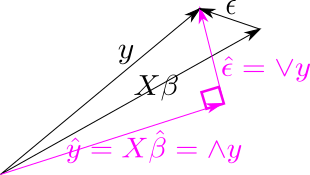
\includegraphics[width=2in]
{conventions/lin-reg-vecs.png}
\caption{Triangles
representing
$y=X\beta+\eps$ and $y=\HAT{y}+\HAT{\eps}$.}
\label{fig-lin-reg-vecs}
\end{figure}

\subsubsection{LR Goodness of Fit, $R^2$}


Assume the components of $\eps$
are random with zero mean:

\beq
E[\rveps]=\av{\rveps}=0
\eeq



Assume $X$ and $\beta$ are not random.
This makes $\rvy=X\beta +\rveps$ and $\ul{\HAT{\beta}}=
(X^TX)^{-1}X^T\rvy
$
random.
One finds that

\begin{subequations}
\beq
\av{\rvy}=X\beta
\eeq


\beq
\av{\HAT{\rvy}}=\A
\underbrace{\av{\rvy}}_{X\beta}
=\av{\rvy}
\eeq

\beq
\av{\HAT{\rveps}}=\V
\underbrace{\av{\rvy}}_{X\beta}
=0
\eeq

\beq
\av{\ul{\HAT{\beta}}}=\beta
\eeq


So far, we have
assumed a zero mean value for $\eps$.
Next, assume
{\bf  ``homoscedasticity" (homo-spread)}\footnote{I
 find the word ``homoscedasticity"
unnecessarily long, cryptic
and easy to misspell so
I like to replace
it by ``homo-spread".
The opposite
of ``homoscedasticity"
is ``heteroscedasticity",
which I like to replace with ``hetero-spread".}, which
means that

\beq
\av{\rveps, \rveps^T}=\xi^2 I_{nsam}
\eeq
\end{subequations}
where
$\xi\geq 0$,  and
$I_{nsam}$ is the
$nsam\times nsam$ identity matrix.
It follows that

\begin{subequations}
\label{eq-lin-re-variances}
\beq
\av{\rvy, \rvy^T}=
\av{\rveps, \rveps^T}=
\xi^2 I_{nsam}
\;,
\eeq

\beq
\av{\HAT{\rveps},
\HAT{\rveps}^T}=
\V\av{\rvy, \rvy^T}\V^T=\xi^2\V
\label{eq-homo}
\;,
\eeq

\beq
\av{\HAT{\rvy},
\HAT{\rvy}^T}=
\A\av{\rvy, \rvy^T}\A^T=\xi^2\A
\eeq
and

\beq
\av{\HAT{\ul{\beta}},
\HAT{\ul{\beta}}^T}=
B\av{\rvy, \rvy^T}B^T=\xi^2 (X^TX)^{-1}
\;.
\eeq
\end{subequations}

For any random column vector $\rva$,
let

\beq
\norm{\rva}^2= \rva^T\rva=\tr(\rva\rva^T)
\eeq
and

\beq
\av{\norm{\rva-\av{\rva}}^2}=
\av{\rva^T\rva}-\av{\rva^T}\av{\rva}
=
\tr\av{\rva, \rva^T}
\;.
\eeq

Define the following sums of squares (SS):

\begin{subequations}
\label{eq-lin-reg-ss}
\beq
SS_{\rvy}=\av{\norm{\rvy-\av{\rvy}}^2}
=\av{\rvy^T\rvy}-\av{\rvy^T}\av{\rvy}
=\tr\av{\rvy,\rvy^T}
\eeq

\beq
SS_{\HAT{\rvy}}=\av{\norm{\HAT{\rvy}-\av{\HAT{\rvy}}}^2}
=\av{\HAT{\rvy}^T\HAT{\rvy}}-\av{\HAT{\rvy}^T}\av{\HAT{\rvy}}
=\tr\av{\HAT{\rvy},\HAT{\rvy}^T}
\eeq

\beq
SS_{res}=\av{\norm{\rvy-\HAT{\rvy}}^2}
=
\av{\norm{\ul{\HAT{\eps}}}^2}
=\tr\av{\ul{\HAT{\eps}},\ul{\HAT{\eps}}^T}
\eeq
\end{subequations}

\begin{claim}
The following is true
without homo-spread:


\beq
\underbrace{\tr\av{\rvy,\rvy^T} }_{SS_\rvy}
=
\underbrace{\tr\av{\HAT{\rvy}, \HAT{\rvy}^T}}_{SS_{\HAT{\rvy}}}
+
\underbrace{\tr\av{\HAT{\rveps}, \HAT{\rveps}^T}}_{SS_{res}}
\eeq
This is like the Pythagorean Theorem
for the magenta right triangle
in Fig.\ref{fig-lin-reg-vecs}.
\end{claim}
\proof

From Eqs.\ref{eq-lin-re-variances}
and \ref{eq-lin-reg-ss},
we see that

\beq
SS_\rvy=\tr\av{\rvy,\rvy^T}
\eeq

\beq
SS_{\HAT{\rvy}}=\tr\av{\HAT{\rvy},\HAT{\rvy}^T}
=\tr\av{\A\rvy, \rvy^T}
\eeq

\beq
SS_{res}=\tr\av{\HAT{\rveps}, \HAT{\rveps}^T}
=\tr\av{\V\rvy, \rvy^T}
\eeq
Now use $\A + \V=1$.
\qed


The goodness of fit
for this model
is often measured using  the
{\bf coefficient of determination}
$R^2$. $R^2$  is defined by


\beq
R^2= 1 -\;\frac{SS_{res}}{SS_\rvy}=
\frac{SS_{\HAT{y}}}{SS_\rvy}
=
\frac{\tr \av{\HAT{\rvy},\HAT{\rvy}^T}}
{ \tr \av{\rvy,\rvy^T}}
\eeq
If homo-spread holds, then
$R^2$ reduces to


\beq
R^2 =\frac{\tr\; \A}{nsam}
\;.
\eeq


\subsection{LR, assuming
$x_\s$ are random}
Let

$i_0\in\{0, 1, 2, \ldots, n\}$ :
index that can assume values 0 to $n$

$i\in\{1, 2, \ldots, n\}$ :
index that can assume values 1 to $n$.
$i$ is never equal to 0.


$\rvy\in\RR$:  true value
of dependent y-variable

$\HAT{\rvy}\in\RR$: cfit
of dependent y-variable

$\ul{\eps}\in\RR$: residual



$\rvx_{i}\in \RR$: independent x-variables
for $i\in\{1,\ldots,n\}$

$\beta_0, \beta_i\in\RR$:
regression coefficients

\beqa
\HAT{\rvy}
&=&
\beta_0 +\sum_{j=1}^{n}
\beta_{j} \rvx_j
\\
&=&
\sum_{j_0=0}^{n}\beta_{j_0} \rvx_{j_0}
\;\;(\text{Assume $\rvx_0=1$.})
\eeqa

\beq
\rvy = \HAT{\rvy}+\ul{\eps}
\eeq

\subsubsection{Transforming
expressions
from
non-random to
random $x_\s$ }

Define the following
population averages:


\beq
E_\s[x^\s]=
\frac{1}{nsam}
\sum_\s x^\s
\;,
\eeq

\beq
E_\s[x^\s y^\s]=
\frac{1}{nsam}
\sum_\s x^\s y^\s
\;,
\eeq

\beq
\av{x^\s,y^\s}_\s=
E_\s[x^\s y^\s]-E_\s[x^\s]E_\s[y^\s]
\;.
\eeq


\begin{claim}\label{cl-sigma-to-ran}
If the $x_\s$ are i.i.d. random
variables,

\beq
E_\s[x^\s] =\av{\rvx}
\;
\label{eq-exp-x}
\eeq
\beq
E_\s[x^\s y^\s]
=
\av{\rvx\rvy}
\label{eq-exp-xy}
\eeq

\beq
\av{x^\s,y^\s}_\s
=
\av{\rvx, \rvy}
\label{eq-exp-x--y}
\eeq
\end{claim}
\proof
\beqa
\frac{1}{nsam}
\sum_\s x^\s
&=&
\frac{1}{nsam}
\sum_{x\in S_\rvx}
x
\underbrace{
\sum_\s \indi(x^\s=x)}_
{N(x^\s=x)}
\\
&=&
\sum_{x}x\;P(x)
\\
&=&
\av{\rvx }
\eeqa

\beqa
\frac{1}{nsam}
\sum_\s x^\s y^\s
&=&
\frac{1}{nsam}
\sum_{x\in S_\rvx}
\sum_{y\in S_\rvy}
xy
\underbrace{
\sum_\s \indi(x^\s=x, y^\s=y)}_
{N(x^\s=x, y^\s=y)}
\\
&=&
\sum_{x,y}xy\;P(x,y)
\\
&=&
\av{\rvx \rvy}
\eeqa
Eq.(\ref{eq-exp-x--y})
follows from
Eq.(\ref{eq-exp-x}) and Eq.(\ref{eq-exp-xy}).
\qed

Recall that

\beq
Y_\s = \beta_0 +  \sum_{j=1}^n X_{\s,j}\beta_j + \eps_\s
\;.
\eeq

Assume
\beq
E_\s[X_{\s,k} \eps_\s]=E_\s[X_{\s,k}]
\underbrace{E_\s[ \eps_\s]}_{=0}=0
\;.
\eeq
Then we have

\beq
E_\s[X_{\s,k} Y_\s]=
E_\s[X_{\s,k}]\beta_0 + \sum_{j=1}^n
E_\s [X_{\s,k} X_{\s,j}] \beta_j +
\underbrace{E_\s[X_{\s,k} \eps_\s]}_{=0}
\label{eq-EXY}
\eeq
and

\beq
E_{\s'}[X_{\s',k}]E_\s[ Y_\s]=
E_{\s'}[X_{\s',k}]\beta_0 + \sum_{j=1}^n
E_{\s'} [X_{\s',k}] E_\s[ X_{\s,j}] \beta_j +
\underbrace{E_{\s'}[X_{\s',k}]  E_\s[ \eps_\s]}_{=0}
\label{eq-EX-EY}
\;.
\eeq
Subtracting
Eq.(\ref{eq-EX-EY}) from Eq.(\ref{eq-EXY}), we get

\beq
\av{X_{\s,k} ,Y_\s}_\s=
\sum_{j=1}^n
\av{X_{\s,k}, X_{\s,j}}_\s \beta_j
\label{eq-avX-comma-Y}
\;.
\eeq
Define the $n$ dimensional
covariance matrix $C$
by

\beq
C_{k,j}=\av{X_{\s,k}, X_{\s,j}}_\s
\:.
\eeq
Then Eq.(\ref{eq-avX-comma-Y}) implies

\beq
\beta_j =\sum_{k=1}^n
C^{-1}_{j,k} \av{X_{\s,k} ,Y_\s}_\s
\label{eq-beta_j-c-inv}
\eeq
for all $j=1,2,\ldots, n$.

If we assume that the $x_\s$ are i.i.d.,
then, by  virtue of Claim \ref{cl-sigma-to-ran},
the matrix $C$ tends to


\beq
C_{k,j}
\rarrow \av{\rvx_k, \rvx_j}
\eeq
and Eq.(\ref{eq-beta_j-c-inv})
implies

\beq
\beta_j = \sum_{k=1}^n C^{-1}_{j,k}\av{\rvx_k, \rvy}
\label{eq-beta-random-from-nonrandom}
\;.
\eeq

\subsubsection{Geometry of LR with random $x_\s$}
Recall that

\beq
\rvy =
\underbrace{\beta_0 +\sum_{j=1}^{n}
\beta_{j} \rvx_j}_{\HAT{\rvy}}
+\ul{\eps}
\;.
\eeq


Assume

\beq
\av{\rveps}=0
\eeq
and
\beq
\av{\rvx_j, \ul{\eps}}=0
\eeq
for all $j$.

For $k=1, \ldots, n$,
\beq
\av{\rvx_k, \rvy}
=
\sum_{j=1}^{n}\beta_j\av{\rvx_k, \rvx_j}
\;.
\label{eq-beta-0-wrong}
\eeq

Let $\rvx^n$ and $\beta^n$ be
$n$-dimensional column vectors.
Then Eq.(\ref{eq-beta-0-wrong})
can be represented
 in matrix notation by
\beq
\av{\rvx^n, \rvy}=
\av{\rvx^n, (\rvx^n)^T}\beta^n
\;.
\eeq
Hence,

\beq
\boxed{
\beta^n=
\av{\rvx^n, (\rvx^n)^T}^{-1}
\av{ \rvx^n, \rvy}
\;.}
\label{eq-beta-random-lin-reg}
\eeq
For $\beta_0$, use

\beq
\beta_0=
\av{\rvy}-\av{\rvx^n}^T \beta^n
\eeq

Notice that
Eq.(\ref{eq-beta-random-lin-reg})
for the regression coefficients
is the same
as Eq.(\ref{eq-beta-random-from-nonrandom}).
So we have rederived the same formula
via a different method.


Next, we will
write
 Eq.(\ref{eq-beta-random-lin-reg})
for the special cases
$n=1$ and $n=2$,
where $n$ is the
number of independent x-variables $\rvx_j$

\begin{enumerate}
\item $n=1$ ($\rvy$ fitted by a line)

\beq
\rvy = \beta_0 + \beta_1\rvx + \rveps
\eeq

Eq.(\ref{eq-beta-random-lin-reg}) becomes
\beq
\beta_1=
\frac{\av{\rvy,\rvx}}{\av{\rvx,\rvx}}
\eeq


\item $n=2$ ($\rvy$ fitted by a plane)


\beq
\rvy = \beta_0 + \beta_1 \rvx_1 + \beta_2 \rvx_2 +\rveps
\eeq
Define


\beq
C_{i,j}=\av{\rvx_i, \rvx_j}
\eeq
for all $i,j$.
Then Eq.(\ref{eq-beta-random-lin-reg})
becomes\footnote{
Recall that if
$
M=
\left[
\begin{array}{cc}
a&b
\\
c&d
\end{array}
\right]
$
then
$
M^{-1}
=
\frac{1}{\det M}
\left[
\begin{array}{cc}
d&-b
\\
-c&a
\end{array}
\right]
$
}


\beqa
\left[
\begin{array}{c}
\beta_1
\\
\beta_2
\end{array}
\right]
&=&
C^{-1}
\left[
\begin{array}{c}
\av{\rvy, \rvx_1}
\\
\av{\rvy, \rvx_2}
\end{array}
\right]
\\
&=&
\frac{1}{\det C}
\left[
\begin{array}{cc}
C_{22}&-C_{12}
\\
-C_{21}&C_{11}
\end{array}
\right]
\left[
\begin{array}{c}
\av{\rvy, \rvx_1}
\\
\av{\rvy, \rvx_2}
\end{array}
\right]
\eeqa


Hence,
\beq
\beta_1
=\pder{\rvy}{\rvx_1}=
\frac{
C_{22}\av{\rvy, \rvx_1}
-C_{12}\av{\rvy, \rvx_2}
}
{
C_{11}C_{22}-C_{12}^2
}
\label{eq-beta-lr-plane}
\eeq
Eq.(\ref{eq-beta-lr-plane})
 agrees with
the
value of $\beta_{YX, Z}$ in
Ref.\cite{pearl-lin-reg}
by Pearl,
if  we replace in Pearl's
formulae $X\rarrow \rvx_1$,
$Y\rarrow \rvy$, $Z\rarrow \rvx_2$.


\end{enumerate}

\subsubsection{Regression
 interpreted as differentiation
 of $y$}

Finding the derivative of $y$
with respect to (wrt) $X$
(a.k.a. ``{\bf Regressing $y$ on $X$}")
is finding
$\HAT{\beta}=\frac{d}{dX}
\underbrace{y}_{X\beta}$.

Recall that

\beq
\rvy = \beta_0 + \sum_{k=1}^n \rvx_k \beta_k + \ul{\eps}
\;.
\eeq
Therefore,

\beqa
\av{\rvx_i, \rvy}
&=&
\sum_{k=1}^n \av{\rvx_i, \rvx_k}\beta_k
\\
&=&
 \av{\rvx_i, \rvx_i}\beta_i
+
\sum_{k=1}^n
\indi(k\neq i)
 \av{\rvx_i, \rvx_k}\beta_k
\;.
\eeqa
Hence,

\beq
\beta_i
=
\frac{\av{\rvx_i, \rvy}}
{\av{\rvx_i, \rvx_i}}
-\sum_{k=1}^n
\indi(k\neq i)
\frac{ \av{\rvx_i, \rvx_k}}
{\av{\rvx_i, \rvx_i}}
\beta_k
\;.
\label{eq-beta-i-non-deriv}
\eeq

Let's represent
the linear
operator
$\av{\rvx_i, \rvx_i}^{-1}\av{\rvx_i, \cdot}
$ as a derivative:

\beq
\frac{d\;\cdot}{d\rvx_i}=
\frac{\av{\rvx_i, \cdot}}
{\av{\rvx_i, \rvx_i}}
\;.
\eeq
Eq.(\ref{eq-beta-i-non-deriv})
can be expressed
in derivative notation as:

\beq
\beta_i
=
\frac{d \rvy}
{d\rvx_i}
-\sum_{k=1}^n\indi(k\neq i)
\frac{ d\rvx_k}
{d\rvx_i}
\beta_k
\label{eq-beta-i-deriv}
\eeq
Note that Eq.(\ref{eq-beta-i-deriv})
evokes the formula for differentials:

\beq
d\rvy=
\sum_{k=1}^n \beta_kd\rvx_k
\;.
\eeq

Note also that,
because of the
linearity of the derivative operator,
Eq.(\ref{eq-beta-i-deriv})
implies:

\beq
\beta_i=
\frac{d}
{d\rvx_i}
\left(\rvy
-
\underbrace{\sum_{k=1}^n
\indi(k\neq i)\rvx_k \beta_k
}_{\rvy-\rvx_i\beta_i}
\right)
\label{eq-beta-i-2-steps}
\;.
\eeq

Eq.(\ref{eq-beta-i-2-steps})
can be used to find
$\HAT{\beta}_i$
in two steps:

STEP 1: Regress $\rvy-\rvx_i\beta_i$
on $(\rvx_k)_{k\in \{1,2,
\ldots, n\}- \{ i\}}$.
Get estimates
$(\HAT{\beta}_k)_{k\in \{1,2,
\ldots, n\}- \{ i\}}$.

STEP 2: Regress $\rvy-\sum_{k\neq i} \rvx_k\HAT{\beta}_k$ on $\rvx_i$.
Get estimate $\HAT{\beta}_i$.

Of course, one can also
find $\HAT{\beta}_i$
by regressing $\rvy$
on $(\rvx_k)_{k\in \{1,2,
\ldots, n\}}$, to get
estimates
$(\HAT{\beta}_k)_{k\in \{1,2,
\ldots, n\}}$.

\section{Logistic Regression (LoR)}

Suppose
$x_\s\in \RR^n$,
$y_\s\in \RR$,
and $\Sigma$
is a population
of individuals $\s$.
In general,
a {\bf regression}
is when
we curve-fit a dataset
$\{(x_\s, y_\s):\s\in\Sigma\}$
with a function
$\haty=f(x)$.
In {\bf Linear
Regression (LR)},
which we
discussed earlier,
$f(x)$ is a hyperplane
in $x$.
On the other hand,
in {\bf Logistic Regression (LoR)},
$y_\s\in[0,1]$ and
$f(x)$ is the sigmoid of
a hyperplane in $x$.



More specifically, for LR
we have
Eq.(\ref{eq-LR-start})
which reads as follows:

\beq
y_\s=
\underbrace{
\beta_0 +
\sum_{i=1}^{n} x_{\s i}\beta_{i}
}_{\haty_\s}+ \eps_\s
\quad\text{(LR)}\;.
\eeq
For LoR, we have instead

\beq
p_\s=
\smoid\left(
\beta_0 +
\sum_{i=1}^{n} x_{\s i}\beta_{i} + \eps_\s
\right)
\quad\text{(LoR)}\;,
\eeq
or, equivalently,


\beq
\underbrace{\lodds(p_\s)}
_{\ln \frac{p_\s}{1-p_\s}}=
\underbrace{
\beta_0 +
\sum_{i=1}^{n} x_{\s i}\beta_{i}
}_{\haty_\s} + \eps_\s
\quad\text{(LoR)}\;,
\eeq
where we have used the fact that
$\lodds()$
is the inverse function of $\smoid()$.
Hence, an LoR
fit can be calculated by
collecting a dataset
$\{(x_\s, p_\s):\s\in\Sigma\}$,
transforming that
dataset to the dataset
$\{(x_\s,\lodds( p_\s)):\s\in\Sigma\}$,
and fitting the latter dataset
with a hyperplane.
Let $P(\rvY_\s=1)=p_\s\in [0,1]$.
LoR can be used
for binary
classification
if we define the
binary class
variable $c_\s\in \bool$ by

\beq
c_\s =\indi(P(\rvY_\s=1)>\alp)
\eeq
for some $0<\alp<1$.



\section{Entropy,
 Kullback-Leibler divergence, Cross-Entropy}

For probability distributions $p(x), q(x)$ of $x\in S_\rvx$
\begin{itemize}
\item
Entropy:
\beq
H(p)=-\sum_x p(x)\ln p(x)\geq 0
\eeq

\item
Kullback-Leibler divergence:

\beq
D_{KL}(p\parallel q)=\sum_{x} p(x)\ln \frac{p(x)}{q(x)}\geq 0
\eeq
\item
Cross entropy:
\beqa
CE(p\parallel q) &=& -\sum_x p(x)\ln q(x)\\
&=& H(p) + D_{KL}(p\parallel q)
\eeqa
\end{itemize}

\section{Definition of various
entropies used in Shannon Information Theory}

\begin{itemize}
\item
{\bf (plain) Entropy of $\rvx$}

\beq
H(\rvx) =
-\sum_{x} P(x)\ln P(x)
\eeq
This quantity measures the
spread of $P_\rvx$.
$H(\rvx)\geq 0$
and it vanishes iff $P(x)=\delta(x,x_0)$ (deterministic case)


\item
{\bf Conditional Entropy of $\rvy$ given $\rvx$}

\beqa
H(\rvy|\rvx) &=&
-\sum_{x,y}P(x,y)\ln {P(y|x)}
\\
&=&
H(\rvy,\rvx)-H(\rvx)
\eeqa
This quantity measures  the conditional
 spread
of $\rvy$ given $\rvx$. $H(\rvy|\rvx)\geq 0$.


\item {\bf Mutual Information (MI)
of $\rvx$ and $\rvy$}.

\beqa
H(\rvy:\rvx) &=&
\sum_{x,y} P(x,y) \ln \frac{P(x,y)}{P(x)P(y)}
\\
&=&
H(\rvx) + H(\rvy) - H(\rvy,\rvx)
\eeqa
This quantity measures the correlation
between $\rvx$ and $\rvy$.
$H(\rvy:\rvx)\geq 0$
and it vanishes iff
$P(x,y)=P(x)P(y)$.

\item {\bf Conditional Mutual Information
(CMI)\footnote{CMI
can be read as ``see me".}
of $\rvx$ and $\rvy$
given $\ul{\lam}$}


\beqa
H(\rvy:\rvx|\ul{\lam})
&=&
\sum_{x,y, \lam}P(x,y, \lam) \ln
\frac{P(x,y|\lam)}{P(x|\lam)P(y|\lam)}
\\
&=&
H(\rvx|\ul{\lam}) + H(\rvy|\ul{\lam})
- H(\rvy,\rvx|\ul{\lam})
\eeqa

This
quantity measures the conditional correlation
of $\rvx$ and $\rvy$ given $\ul{\lam}$.
$H(\rvy:\rvx|\ul{\lam})\geq 0$
and it vanishes iff
$P(x,y|\lam)=P(x|\lam)P(y|\lam)$.

An interesting special case
occurs when
$P(\lam)=\delta(\lam, \lam_0)$ (the
frequentist  case of no $\lam$ prior.)
In that case CMI
reduces to

\beq
H(\rvy:\rvx|\lam_0)
=
\sum_{x,y}P(x,y|\lam_0) \ln
\frac{P(x,y|\lam_0)}{P(x|\lam_0)P(y|\lam_0)}\geq 0
\eeq



\item {\bf Kullback-Leibler Divergence
from $P_\rvx$ to $P_\rvy$.}

Assume random variables $\rvx$
and $\rvy$
have the same set of states
$S_\rvx=S_\rvy$. Then


\beq
D_{KL}(P_\rvx\parallel P_\rvy)=
\sum_x P_\rvx(x) \ln \frac{P_\rvx(x)}{P_\rvy(x)}
\eeq

This quantity measures a non-symmetric distance
between the probability distributions
$P_\rvx$ and $P_\rvy$.
$D_{KL}(P_\rvx\parallel P_\rvy)\geq 0$
and it equals zero iff $P_\rvx=P_\rvy$.

\end{itemize}

\section{Mean log likelihood asymptotic behavior}
\label{sec-ent-like-connect}

Define the log likelihood  by
\beq
 LL_{y|\theta} = \ln P(y|\theta)
\;.
\eeq
In this section, we will represent averages over $\rvy|\theta$ by
angular brackets:
\beq
\av{f(y)}= \sum_y P(y|\theta) f(y)= E_{\rvy|\theta}[f(y)]
\;.
\eeq
Note that the mean log likelihood equals minus the entropy:

\beq
H(\rvy|\theta)= -\av{ LL_{y|\theta}}
\eeq

\begin{claim}

\beq
\av{\partial_\theta   LL_{y|\theta}}=0
\eeq

\beq
\av{\partial^2_\theta   LL_{y|\theta}}=
-\av{ (\partial_\theta  LL_{y|\theta})^2 }
\eeq

\end{claim}
\proof

\beqa
\av{\partial_\theta   LL_{y|\theta}}
&=&
\sum_y P(y|\theta)\partial_\theta\ln  P(y|\theta)
\\
&=&
\sum_y \partial_\theta P(y|\theta)
\\
&=& 0
\eeqa


\beqa
\av{\partial^2_\theta   LL_{y|\theta}}
&=&
\sum_y  P(y|\theta)\partial_\theta \left[ \frac{1}{P(y|\theta)}
 \partial_\theta P(y|\theta) \right]
\\
&=&
- \sum_y  P(y|\theta)
\frac{1}{P(y|\theta)^2}[ \partial_\theta P(y|\theta)]^2
+  \underbrace{ \sum_y   \partial_\theta^2   P(y|\theta)}_{=0}
\\
&=&
-\sum_y  P(y|\theta)[ \partial_\theta \ln P(y|\theta)]^2
\\
&=&
-\av{ (\partial_\theta  LL_{y|\theta})^2 }
\eeqa
\qed

Define
\beq
\Delta \theta =  \theta' - \theta
\eeq
and

\beq
-\Delta H(\rvy|\theta)=
\Delta\av{  LL_{y|\theta}}
=
\av{  LL_{y|\theta'}}-
\av{  LL_{y|\theta}}
\;
\eeq
If we expand
$\av{  LL_{y|\theta'}}$ as a Taylor series
to second order
about the point $\theta'=\theta$,
we get


\beq
\av{  LL_{y|\theta'}}=
\av{  LL_{y|\theta}}
+
\Delta \theta
\underbrace{\av{ \partial_\theta LL_{y|\theta}}}_{=0}
+
\frac{(\Delta\theta)^2}{2}
\underbrace{\av{ \partial^2_\theta LL_{y|\theta}}}_
{-\av{ (\partial_\theta LL_{y|\theta})^2} }
+ \calo((\Delta\theta)^3)
\eeq

\beq
-\Delta H(\rvy|\theta)=\Delta\av{  LL_{y|\theta}}
=
-\;\frac{(\Delta\theta)^2}{2}
\av{ (\partial_\theta LL_{y|\theta})^2}
+ \calo((\Delta\theta)^3)
\eeq
Thus, $\theta'=\theta$ maximizes
the mean log likelihood $\av{  LL_{y|\theta}}$
(and minimizes the entropy $H(\rvy|\theta)$).

Note that
\beq
\Delta\av{  LL_{y|\theta}}
=
\av{\ln \frac{P(y|\theta')}{P(y|\theta)}}
\;.
\eeq
If we approximate
the ratio of these 2 probabilities by a Gaussian,

\beq
\frac{P(y|\theta')}{P(y|\theta)}
\approx \exp \left(-\;\frac{(\Delta \theta)^2}{2\s^2_\theta}\right)
\;,
\eeq
then

\beq
\s^2_\theta = \av{ (\partial_\theta LL_{y|\theta})^2}^{-1}
\;.
\eeq


\section{Arc Strength (Arc Force)}

Given a bnet with an arc (i.e., arrow) $\rvx\rarrow \rvy$,
we define the {\bf arc strength or arc force}
of arc $\rvx\rarrow \rvy$
to be
$H(\rvx:\rvy)$ (i.e., the mutual information between $\rvx$ and
$\rvy$). Evaluation of $H(\rvx:\rvy)$ requires knowing
$P(y|x)$, $P(x)$ and $P(y)$.
$P(y|x)$ is the TPM of node $\rvy$, so it is immediately
available from the specification of the bnet.
Calculating $P(x)$ and $P(y)$ is more involved,
and  requires marginalizing the full probability
distribution of the bnet. Such marginalizations can be
done using the junction tree algorithm described in
Chapter \ref{ch-junc-tree}.


\section{Pearson Chi-Squared Test}

The
{\bf Pearson divergence}
(a.k.a. {\bf Pearson Chi-squared test statistic})
for two
probability distributions
$PO(x)$ and $PE(x)$,
where $x\in S_\rvx$,
is defined
as follows:
\beq
D_{\chi^2}=
\sum_x
\frac{[PO(x)-PE(x)]^2}{PE(x)}
=
\sum_x \frac{PO^2(x)}{PE(x)}-1
\;.
\eeq
Usually $PO$ is the
observed probability distribution and
$PE$ is the expected, theoretical one.

As the following claim shows,
the Pearson divergence
is closely related to the
Kullback-Leibler divergence.


\begin{claim}
If $\left|\frac{PO(x)}{PE(x)}-1\right|<<1$
for all $x\in S_\rvx$, then

\beq
D_{KL}(PO\parallel PE)\approx D_{\chi^2}
\;.
\eeq
\end{claim}
\proof
\beqa
D_{KL}(PO\parallel PE)
&=&
\sum_x PO(x)\ln \frac{PO(x)}{PE(x)}
\\
&=&
\sum_x PO(x)\ln
\left(1 + \frac{PO(x)}{PE(x)} -1
\right)
\\
&\approx&
\sum_x
PO(x)\left(
\frac{PO(x)}{PE(x)} -1
\right)
\\
&=&
\sum_x
\frac{PO^2(x)}{PE(x)} -1
\\
&=&
D_{\chi^2}
\eeqa
\qed

Let $nx=|S_\rvx|$.
Let $P_{\chi^2}(y)$
be the $\chi^2$
(with $nx-1$ degrees of freedom)
probability
distribution,
and let $F_{\chi^2}(\alp)$
be its cumulative
distribution.
Find $\alp$
such that
\beq
95\%=\int_{0}^{\alp}dy\; P_{\chi^2}(y)=
F_{\chi^2}(\alp)
\eeq
If $D_{\chi^2}<\alp$,
then we say that $PO=PE$ to 95\%
significance level (SL),
whereas if
$D_{\chi^2}>\alp$,
we say that $PO\neq PE$
to 95\% SL (i.e., SL$=95\%$).
The higher SL becomes,
the higher $\alp$ becomes,
and the bigger the
divergence $D_{\chi^2}$
has to be,
before we are
willing to declare that $PO\neq PE$.

\section{Demystifying Population
and Sample Variances}
Let $x[\s]=x^\s$.
Given  i.i.d.real  variables
$(x^\s)_{\s=0,1, \ldots, n-1}$,
let\footnote{Do not confuse the sample
index $\s$ and the standard deviation
$\s$.}

\beq
\HAT{\mu}=\ol{x}=
\frac{1}{n}
\sum_\s x^\s
\;
\eeq

\beq
(\hatvar)_\infty=
\frac{1}{n}
\sum_\s (x^\s-\mu)^2
\eeq

\beq
\hatvar=
\frac{1}{n-1}
\sum_\s (x^\s-\HAT{\mu})^2
\eeq

Statisticians\footnote{
In the language of Statisticians,
 a ``population"
is supposed to be
so large that its $\mu$
does not fluctuate,
and a ``sample" is
supposed to be a small
subset of that population
for which the $\mu$
is assumed to fluctuate.
In this book, I
use the word ``population"
to mean a set of any size
containing individuals, I use
the word ``sub-population"
to refer to a subset
of the population,
and I use the
word ``sample"
(a.k.a. individual, observation, unit,
record)  to mean a
single individual
of the population.} call
$(\hatvar)_\infty$ the
``population variance". I will
call it the {\bf population
variance for fixed $\mu$}.
Note that it depends
on
the fixed parameter $\mu$.
Statisticians   call
$\hatvar$ the
``sample variance".
Instead,
 I will
call $\hatvar$ the {\bf
population
variance for random $\mu$}.

If one treats $x^\s$ as a random
variable, then one must treat
$\HAT{\mu}$
as a random variable too.
Let
\beq
E[\rvx^\s]=\mu
\eeq
and

\beq
\av{\rvx^\s, \rvx^{\s'}}=
\delta(\s, \s')\s^2
\;.
\eeq
Then one can show that

\beqa
E[\ul{(\hatvar)_\infty}]
&=&
\frac{1}{n}
E\left[
\sum_\s (\rvx^\s-\mu)^2
\right]
\\
&=&
\s^2
\eeqa
and

\beqa
E[\ul{\hatvar}]
&=&
\frac{1}{n-1}
E\left[
\sum_\s (\rvx^\s-\HAT{\ul{\mu}})^2
\right]
\\
&=&
\s^2
\eeqa
This is the
reason
why
we use
an $n-1$
instead
of an $n$
in $\hatvar$.
Because it
makes
$E[\hatvar]=\s^2$
so
$\hatvar$
is an
unbiased estimator of
the single individual variance $\s^2$.

The intuitive reason for
why $\hatvar$
is divided
by $n-1$
instead of $n$
is that whereas $\mu$
in $(\hatvar)_\infty$
is kept fixed
and is ``quiet",
the $\ul{\HAT{\mu}}$
in  $\hatvar$
is a random variable,
noisy instead of quiet.
The fluctuations in
$\ul{\HAT{\mu}}$
are strongly
correlated with
the fluctuations
of the $\rvx^\s$,
so they decrease the
fluctuations  in $\hatvar$
compared to those in
$(\hatvar)_\infty$.
By dividing by $n-1$
instead of $n$,
we compensate for this
decrease in fluctuations
so that the ratio
of the numerator
and denominator
of  $\hatvar$
equals $\s^2$,
instead of something
{\it smaller} than $\s^2$,
as would happen if were to divide
by $n$ instead of $n-1$.
In terms of ``degrees of freedom"(DOFs),
$(\hatvar)_\infty$ has $n$ DOFs
(namely one for each $\rvx^\s$),
whereas $\hatvar$
has $n-1$ DOFs.
(the presence of $\ul{\HAT{\mu}}$
subtracts one DOF).
In both $(\hatvar)_\infty$
and $\hatvar$,
one divides by the number of DOFs.

\section{Independence of $\widehat{\mu}$
and $\widehat{\sigma^2}$} % hyperrefs can't take \HAT
\label{sec0-ind-mu-sig-hat}

Let $x[\s]=x^\s$.
Consider i.i.d.real  variables
$(x^\s)_{\s=0,1, \ldots, n-1}$
such that\footnote{Do not confuse the sample
index $\s$ and the standard deviation
$\s$.}
\beq
E[\rvx^\s]=\mu
\eeq

\beq
\av{\rvx^\s, \rvx^{\s'}}=
\delta(\s, \s')\s^2
\;.
\eeq

\beq
\HAT{\mu}=\ol{x}=
\frac{1}{n}
\sum_\s x^\s
\;
\eeq

\beq
(\hatvar)_\infty=
\frac{1}{n}
\sum_\s (x^\s-\mu)^2
\eeq

\beq
\hatvar=
\frac{1}{n-1}
\sum_\s (x^\s-\HAT{\mu})^2
\eeq


\begin{claim}\label{claim-3Delta}
Let
\beq
\rvDel^\s= \rvx^\s-\mu
\;.
\eeq
For any $\s_1, \s_2, \s_3$,
\beq
\av{\rvDel^{\s_1}\rvDel^{\s_2}, \rvDel^{\s_3}}=0
\;.
\eeq
\end{claim}
\proof

Suppose $\s_2\neq\s_3$.
Then

\beq
\av{\rvDel^{\s_1}\rvDel^{\s_2}, \rvDel^{\s_3}}
=\underbrace{\av{\rvDel^{\s_2}}}_{0}
\av{\rvDel^{\s_1}, \rvDel^{\s_3}}
=0
\;.
\eeq
So assume $\s_2=\s_3=\s$
and evaluate
$\av{\rvDel^{\s_1}\rvDel^{\s}, \rvDel^{\s}}$.

Suppose $\s_1\neq \s$. Then
\beq
\av{\rvDel^{\s_1}\rvDel^{\s}, \rvDel^{\s}}=
\underbrace{\av{\rvDel^{\s_1}}}_{0}
\av{\rvDel^{\s}, \rvDel^{\s}}=0
\;.
\eeq
So suppose $\s_1=\s$ and evaluate
$\av{(\rvDel^{\s})^2, \rvDel^{\s}}$.

\beq
\av{(\rvDel^{\s})^2, \rvDel^{\s}}=
\underbrace{\av{(\rvDel^\s)^3}}_0
-\av{(\rvDel^\s)^2}
\underbrace{\av{\rvDel^\s}}_0=0
\;.
\eeq
\qed

\begin{claim}
\beq
\av{ \HAT{\ul{\s^2}}, \HAT{\rvmu}}=0
\;.
\eeq
\end{claim}
\proof
\beqa
\av{ \HAT{\ul{\s^2}}, \HAT{\rvmu}}
&=&\frac{1}{n(n-1)}
\sum_{\s, \s'}\av{
\left(\rvx^\s-\;\frac{1}{n}\sum_{\s''}\rvx^{\s''}\right)^2,
\rvx^{\s'}}
\\
&=&\frac{1}{n(n-1)}
\sum_{\s, \s'}\av{
\left(\rvx^\s-\;\frac{1}{n}\sum_{\s''}\rvx^{\s''}\right)^2,
\rvDel^{\s'}}
\\
&=&\frac{1}{n(n-1)}
\sum_{\s, \s'}\av{
\left(\rvDel^\s-\;\frac{1}{n}\sum_{\s''}\rvDel^{\s''}\right)^2,
\rvDel^{\s'}}
\\
&=&0\;\;\;\; \text{by Claim \ref{claim-3Delta}}
\;.
\eeqa
\qed

\section{Chi-square distribution}
This section
is based on Ref.\cite{wiki-chi-sq}.

\begin{figure}[h!]
$$
\xymatrix{
\rvq&\rvz.\ar[l]
}
$$
\caption{Bnet
used to define the Chi-square distribution.}
\label{fig-chi-sq}
\end{figure}

Let $q\in\RR$ and
$z.=\{z_i\}_{i=0,1, \ldots, \nu-1}$
where $z_i\in \RR$.
Consider the bnet of Fig.\ref{fig-chi-sq}.
The TPMs, printed in blue,
for that bnet, are as follows:\footnote{
Don't confuse the $q$
independent constant $\caln(!q)$
with the normal probability distribution
$\caln(x;\mu, \s^2)$.}




\beq
\color{blue}
P(z_i)=\caln(z_i; \mu=0, \s^2=1)
\;.
\eeq
We want
\beq
\rvq = \sum_{i=0}^{\nu-1} (\rvz_i)^2
\eeq
so $P(q|z.)$
is a Dirac delta function:

\beq
\color{blue}
P(q|z.)=\delta(
q - \sum_{i=0}^{\nu-1} (z_i)^2
)
\;.
\eeq
Therefore

\beqa
P(q) &=& \prod_{i=0}^{\nu-1}\left\{\int dz_i
\;P(z_i)
\right\}P(q|z_.)
\\
&=&
\caln(!q)q^{\frac{\nu}{2}-1}e^{-q/2}=\chi^2(q;\nu)
\;,
\eeqa
where $\caln(!q)$ is a constant that does not depend
on $q$ and is adjusted so that $\int_0^\infty dq\;P(q)=1$.

\section{Student's t-distribution}
This section
is based on Ref.\cite{wiki-stud}.

Let $x[\s]=x^\s$.
Consider i.i.d.real  variables
$(x^\s)_{\s=0,1, \ldots, n-1}$
such that\footnote{Do not confuse the sample
index $\s$ and the standard deviation
$\s$.}

\beq
E[\rvx^\s]=\mu
\eeq

\beq
\av{\rvx^\s, \rvx^{\s'}}=
\delta(\s, \s')\s^2
\;.
\eeq

\beq
\HAT{\mu}=\ol{x}=
\frac{1}{n}
\sum_\s x^\s
\;
\eeq

\beq
(\hatvar)_\infty=
\frac{1}{n}
\sum_\s (x^\s-\mu)^2
\eeq

\beq
\hatvar=
\frac{1}{n-1}
\sum_\s (x^\s-\HAT{\mu})^2
\;.
\eeq

If we define

\beq
z =
\frac{\HAT{\mu}-\mu}{\frac{\s}{\sqrt{n}}}
\label{eq-conv-zdef}
\;,
\eeq
then $\rvz$ has a Standard Normal
 Distribution (SND):

\beq
P(z)=\frac{1}{\sqrt{2\pi}}e^{-\;\frac{x^2}{2}}=\caln(z;\mu=0, \s^2=1)
\eeq
But what if we allow the standard deviation $\s$
to fluctuate in the expression
Eq.(\ref{eq-conv-zdef}) for $z$?
Define

\beq
t =
\frac{\HAT{\mu}-\mu}{\sqrt{\frac{\HAT{\s^2}}{n}}}
\;.
\label{eq-conv-tdef}
\eeq
Then one can show that
$\rvt$
has the {\bf Student's t-distribution}
${\rm Stud}(t;\nu=n-1)$
given by:

\beq
P(t)=
\caln(!t)
(1+\frac{t^2}{\nu})^{-\;\frac{\nu+1}{2}}=\text{Stud}(t;\nu=n-1)
\eeq

Note that if we use the approximation
$e^x\approx 1 +x +\calo(x^2)$,
we can show that ${\rm Stud}(t)$
tends to the SND
when $n>>1$:

\beqa
P(t)&=&\caln(!t)
(1+\frac{t^2}{\nu})^{-\;\frac{\nu+1}{2}}
\\
&\approx&
\caln(!t)e^{-\;\frac{t^2}{2}\frac{\nu+1}{\nu}}
\\
&\approx&
\caln(t; \mu=0, \s^2=1)
\;.
\eeqa

\hrule\noindent {\bf Partial derivation
of the explicit
form of ${\rm Stud}(t)$.}

Note that the $z$ definition
Eq.(\ref{eq-conv-zdef})
and the $t$ definition
Eq.(\ref{eq-conv-tdef}),
imply that
\beq
t= z
\underbrace{\sqrt{\frac{\s^2}{\HAT{\s^2}}}}_{\varrho}
\;,
\eeq
In the
expression $\rvt=\rvz\ul{\varrho}$,
the
 random variables
$\rvz$ and $\ul{\varrho}$
are independent
because, as shown in Section
[\nameref{sec0-ind-mu-sig-hat}],
 $\HAT{\mu}$
and $\HAT{\sigma^2}$
are independent.
Therefore, the random variable $\rvt$
can be defined using the bnet
of Fig.\ref{fig-stud-bnet}.

\begin{figure}[h!]
$$
\xymatrix{
&\ul{\varrho}\ar[ld]
\\
\rvt&\rvz\ar[l]
}
$$
\caption{Bnet used to define
the Student's t-distribution.}
\label{fig-stud-bnet}
\end{figure}
The TPMs, printed in blue,
for the bnet Fig.\ref{fig-stud-bnet},
are as follows:

\beq\color{blue}
P(t|z, \varrho)=
\delta(t- z\varrho)
\;\;\;\text{(Dirac delta function)}
\eeq

\beq\color{blue}
P(z)=\caln(z; \mu=0, \s^2=1)
\eeq

\beq\color{blue}
P(\varrho)=\text{given by
 Eq.(\ref{eq-stud-rho-pd}) below.}
\eeq

Note that
\beqa
P(\rvt=t)&=&
P(\rvz\ul{\varrho}=t)
\\
&=&
\int d\varrho\;
P(\rvz=\frac{t}{\varrho}|\varrho)P(\varrho)
\\
&=&\int d\varrho\;
\caln(\frac{t}{\varrho}; 0, 1)P(\varrho)
\\
&=&\int d\varrho\;
\frac{1}{\sqrt{2\pi}}
e^{-\;\frac{1}{2}(\frac{t}{\varrho})^2}P(\varrho)
\;.
\eeqa
If we define $q$ by

\beq
q =\frac{n-1}{\varrho^2}
\;,
\label{eq-stud-def1-q}
\eeq
then

\beq
q=\frac{(n-1)\hatvar}{\s^2}
=
\frac{1}{\s^2}
\sum_{\s=0}^{n-1}(x^\s-\HAT{\mu})^2
\;.
\label{eq-stud-def2-q}
\eeq
As a consequence of
``Cochran's Theorem"
(see Ref.\cite{wiki-coch-theo}),
$\rvq$ given
by Eq.(\ref{eq-stud-def2-q}) must have
a Chi-square probability
distribution with $\nu=n-1$
degrees of freedom:\footnote{Note
that this $q$
is a quadratic form
$q=\vec{x}^T M \vec{x}$,
where $\vec{x}$ is an $n$ dimensional
column vector with components
$x^\s$,
and $M$ is an $n\times n$ matrix.
Cochran's Theorem
diagonalizes $M$
and replaces the
vectors $\vec{x}$
by equivalent ones in a new
basis.
Then the number
of $DOF$s (degrees of freedom)
of the chi-square distribution
is the number of non-zero
diagonal elements in
 the diagonalized $M$
(this
number is called the rank of $M$).
In the particular case of
Eq.(\ref{eq-stud-def2-q}),
$DOF=n-1$.}

\beq
P(q)= \chi^2(q;\nu=n-1)
\eeq

Henceforth, let $\nu=n-1$.
From the definition
Eq.(\ref{eq-stud-def1-q})
of $q$, we get

\beq
dq=
\frac{-2\nu}{\varrho^3}d\varrho
\;.
\eeq
Therefore,


\beqa
P(\varrho)d\varrho
&=&
P(q)dq
\\
&=&
\chi^2(\frac{\nu}{\varrho^2};\nu)\frac{(-2\nu)}{\varrho^3}d\varrho
\\
&=&
\caln(!\varrho)
\left(\frac{\nu}{\varrho^2}\right)
^{\frac{\nu}{2}-1}e^{-\;\frac{\nu}{2\varrho^2}}
\frac{d\varrho}{\varrho^3}
\\
&=&\caln(!\varrho)
\frac{d\varrho}
{\varrho^{\nu+1}}e^{-\;\frac{\nu}{2\varrho^2}}
\;.
\label{eq-stud-rho-pd}
\eeqa
Hence,

\beqa
P(t)&=&\caln(!t)
\int_0^\infty
\frac{d\varrho}
{\varrho^{\nu+1}}e^{-\;\frac{\nu}{2\varrho^2}}
e^{-\;\frac{1}{2}(\frac{t}{\varrho})^2}
\\
&=&\caln(!t)
\int_0^\infty
\frac{d\varrho}
{\varrho^{\nu+1}}
e^{-\;\frac{1}{2}\frac{t^2+\nu}{\varrho^2}}
\;.
\eeqa

\section{Hypothesis testing and 3 classic test statistics
(Likelihood, Score, Wald)}

Suppose we have
data $\vec{x}=[x^\s]_{\s=0, 1, \ldots,
nsam-1}$ which is distributed
according to
a probability distribution
$P(\vec{x};\theta)$
which depends
on some parameters $\theta=
(\theta_i)_{i=0, 1, \ldots,n-1}\in \RR^n$.
We define the
\begin{itemize}
\item
{\bf Likelihood of $\theta$} by

\beq
L(\theta)=P(\vec{x}|\theta)
\;,
\eeq
\item
the {\bf Maximum Likelihood estimate
of $\theta$} by

\beq
\HAT{\theta}=\argmax_\theta L(\theta)
\;,
\eeq
\item
the
{\bf log likelihood of $\theta$} by

\beq
LL(\theta) =\ln L(\theta)
\;,
\eeq
\item
the {\bf Score} or {\bf Lagrange
Multiplier vector}\footnote{$sc_i(\theta)=
\partial_{\theta_i}LL(\theta)$
is called a Lagrange multiplier
because to maximize $LL(\theta)$
over $\theta$ subject to
the constraint $\theta=\theta^*$,
we maximize
the Lagrangian $\call= LL(\theta)
-\sum_i \alp_i[\theta_i - \theta^*_i]$ over
$(\theta_i,\alp_i)$ for all $i$. The latter
gives $\alp_i=\partial_{\theta_i}LL(\theta^*)$
and $\theta=\theta^*$.
For a general
constrained optimization
problem, $\call=LL(\theta)-\sum_i \alp_ic_i(\theta)$
for some constraint functions $c_i(\theta)$.
Hence, $\alp_i=\partial_{\theta_i}LL/
\partial_{\theta_i}c_i$
and $c_i(\theta)=0$
for all $i$.
So, in general,
a Lagrange multiplier
is a ratio of two partial
derivatives.} of $\theta$ by

\beq
sc(\theta)=[sc_i(\theta)]\in \RR^n
\;,
\eeq
where

\beq
sc_i(\theta)=\partial_{\theta_i}LL(\theta)
\;,
\eeq
\item
and the
{\bf Fisher Information Matrix
of $\theta$} by

\beq
FI(\theta)= [FI_{i,j}(\theta)]\in \RR^{n\times n}
\eeq
where
\beq
FI_{i,j}(\theta)
=-
E_{\vec{\rvx}|\theta}
[
\partial_{\theta_i}\partial_{\theta_j}
\overbrace{
\ln P(\vec{\rvx}|\theta)}^{LL(\theta)}
]
\;.
\eeq
\end{itemize}

Note that if

\beq
LL(\theta)=\ln P(x|\theta)=
 \frac{-(\theta
-\HAT{\theta})^2}{2\s^2} + \caln(!\theta)
\;,
\label{eq-normal-ll}
\eeq
then

\beq
sc(\theta)=\frac{-(\theta-\HAT{\theta})}{\s^2}
\eeq
and

\beq
FI(\theta)=\frac{1}{\s^2}
\eeq



In hypothesis testing, one has
 a {\bf null hypothesis}
$H_0$: $\theta=\theta^*$,
and an {\bf alternative hypothesis}
 $H_1$: $\theta\neq \theta^*$.
We use a {\bf test statistic}
$\lam(\theta^*, \HAT{\theta})\geq 0$
which
measures a kind of
distance or separation between the
estimate $\HAT{\theta}$
and
the value $\theta^*$
for the null Hypothesis $H_0$.
For some {\bf confidence level} $C>0$,
if $\lam(\theta^*, \HAT{\theta})> C$,
$H_0$ is {\bf rejected}, whereas
if $\lam(\theta^*, \HAT{\theta})\leq C$,
$H_0$ is {\bf accepted}.


$\alp=1-C$ is called the
{\bf significance level}.
Usually $\alp<<1$
represents
the area under both
tails
of a Normal
distribution,
 and $C\approx 1$
represents
all the area except the tails of a
Normal distribution.

\begin{figure}[h!]
\centering
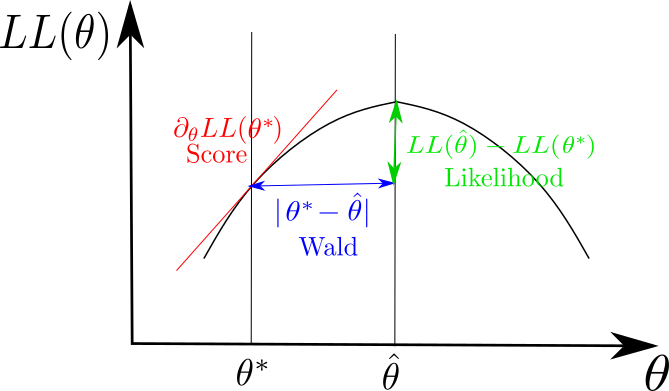
\includegraphics[width=3.2in]{conventions/classic-trio.png}
\caption{For $n=1$ and $\theta\in\RR$,
this figure shows the geometrical significance of
certain
quantities that
characterize the
3 classic test statistics
(Likelihood, Score, Wald)
for hypothesis testing.}
\label{fig-classic-trio}
\end{figure}

Henceforth in this section,
we will
occasionally  use the
Einstein summation
convention; i.e., implicit sum over
repeated indices.

Three classic test statistics
are (See Fig.\ref{fig-classic-trio}):

\begin{enumerate}

\item
{\bf Likelihood Ratio test statistic}
(Ref.\cite{wiki-Li-test}.)

\beq
\lam_{Li}=
2\ln\left[
\frac{L(\HAT{\theta})}
{L(\theta^*)}
\right]=
2[LL(\HAT{\theta})-LL(\theta^*)]
\eeq

\item
{\bf Score (a.k.a.
Lagrange multiplier) test statistic}
(Ref.\cite{wiki-Sc-test}.)

\beqa
\lam_{Sc}&=&
\partial_{\theta_i} LL(\theta^*)
\left[
FI(\theta^*)^{-1}\right]_{i,j}
\partial_{\theta_j} LL(\theta^*)
\\
&=&
\frac{[\partial_\theta LL(\theta^*)]^2}
{FI(\theta^*)}\quad \text{if $n=1$}
\eeqa
Doesn't depend on $\HAT{\theta}$.

\item
{\bf Wald test statistic}
(Ref.\cite{wiki-Wa-test}.)


\beqa
\lam_{Wa}&=&
(\HAT{\theta}-\theta^*)_i
\left[
\av{\HAT{\rvtheta},\HAT{\rvtheta}^T}^{-1}
\right]_{i,j}
(\HAT{\theta}-\theta^*)_j
\label{eq-wald-stat}
\\
&=&
\frac{(\theta^*-\HAT{\theta})^2}
{\av{\HAT{\theta},\HAT{\theta}}}
\quad\text{if $n=1$}
\eeqa

More generally,
one can replace $\theta^*\rarrow R\theta^*$
and  $\HAT{\theta}\rarrow R\HAT{\theta}$
in Eq.(\ref{eq-wald-stat}),
where $\theta^*$ and
$\HAT{\theta}$ are $n$ dimensional
column vectors, and
$R\in\RR^{\nu\times n}$.
The null and alternative hypotheses become:
$H_0: R\theta=R\theta^*$
and $H_1: R\theta\neq R\theta^*$.
Note that
$\nu$
is the number of
constraints imposed by the
null hypothesis. $R$ is called a
reparametrization of $\theta$.
The Wald test is not
reparametrization
invariant (i.e., $R$
invariant), but the Likelihood Ratio test is.

\end{enumerate}

Note that
if $LL(\theta)$
is given by Eq.(\ref{eq-normal-ll}),
then
$\av{\HAT{\rvtheta},\HAT{\rvtheta}}
=
\s^2=\frac{1}{FI(\theta)}
$. Hence,

\beq
\lam_{Li}=\lam_{Sc}=\lam_{Wa}=
\frac{(\HAT{\theta}-\theta^*)^2}{\s^2}
\eeq

Many
other commonly used test statistics
(or their squares)
are special cases of one
of the 3 classic test statistics.
For example, the z-statistic
used with normal
distributions,
the t-statistic
used with the
Student t-distribution,
the F-statistic used in linear regression,
the chi-squared statistic used
to do Pearson's chi-squared test.

{\bf Asymptotic Behavior}

If the data
$\vec{x}$ is i.i.d.,

\beq
P(\vec{x}|\theta)=
\prod_{\s=0}^{nsam-1} P(x^\s|\theta)
\;
\eeq
Hence, as $nsam\rarrow \infty$,

\beqa
LL(\theta)
&=&
\ln P(\vec{x}|\theta)
\\
&=&\sum_\s \ln
P(x^\s|\theta)
\\
&\rarrow&
nsam \sum_x P(x|\theta)\ln  P(x|\theta)
\\
&=&
-nsam \; H(\rvx|\theta)
\eeqa
Thus, {\it maximizing} the log likehood
$LL(\theta)$
and {\it minimizing} the entropy
$H(\rvx|\theta)$
give the same estimate $\HAT{\theta}$.

When the
data is i.i.d. and
$nsam\rarrow \infty$,
it is also possible to
prove that
the 3 test statistics
defined above all tend to
the same
probability  distribution, namely
$\calx^2(\theta^*; \nu)$,
the chi-square distribution
with $\nu$ degrees of freedom,
where $\theta\in \RR^n$, $R\in \RR^
{\nu\times n}$, and $\nu=n$ if $R=1$.

\section{Error Bars}
Never report measurements without error bars!!

Assume a distribution
with mean $\mu$ and
standard deviation $\s$
for a subpopulation with $n$
samples.

$SE=\frac{\s}{\sqrt{n}}$
is called the {\bf standard error}.


Some popular types of error bars:


\begin{itemize}
\item{\bf Box and Whiskers plot (a.k.a. Boxplot)}

See Fig.\ref{fig-boxplot}.
$IQR$ stands for {\bf
Intermediate Quantile Range}.
Sometimes, the endpoints of the
error bars are taken to be the minimum and maximum samples
instead of $Q_1- 1.5 *IQR$ and $Q_3+ 1.5 *IQR$.
The points that fall
in the intervals $[\min,Q_1- 1.5* IQR]$
and $[Q_3+ 1.5 *IQR, \max]$
are
called {\bf outliers}.
\begin{figure}[h!]
\centering
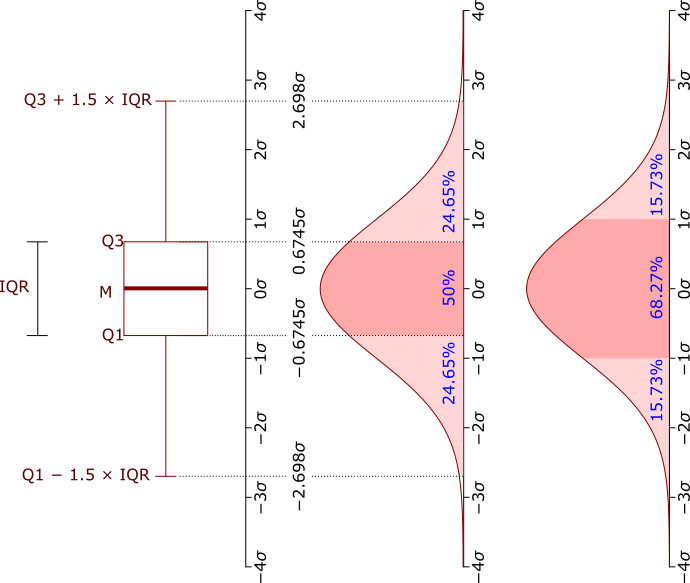
\includegraphics[width=3.3in]
{conventions/Boxplot.png}
\caption{Boxplot plot for Normal
distribution $\caln(\mu=0,\s)$.
$Q_1$ and $Q_3$ are the first and third
quantiles, and $M$ is the median (i.e., half-way point).
For a non-normal skewed
distribution, $Q_1$ and $Q_3$
are not equidistant from the median, and the
median is not exactly equal to the mean. }
 \label{fig-boxplot}
\end{figure}



\item{\bf Standard Deviation}

Error bar endpoints are located one standard deviation
away from the mean.
\beq
\mu-\s< \mu < \mu+\s
\eeq

\item{\bf Confidence Interval}

\beq
\mu-|z^*|SE <\mu < \mu+|z^*|SE
\label{eq-conf-int}
\eeq

$|z^*|=1.96$ for a confidence level of $95\%$.

The origin of Eq.(\ref{eq-conf-int})
is explained in the next section entitled ``Confidence Intervals".
Confidence intervals are
derived from the Gaussian in Fig.\ref{fig-conf-int},
which should not be confused with the
Gaussian of Fig.\ref{fig-boxplot}.
They are different!

\end{itemize}
\section{Confidence Interval}

Normal distribution
with mean $\mu$
and standard deviation $\sigma$:

\beq
\caln(x;\mu, \s^2)=
\frac{1}{\s\sqrt{2\pi}}
e^{-\;\frac{(x-\mu)^2}{2\sigma^2}}
\;.
\eeq

Standard Normal Distribution (SND):
\beq
P(z)=\caln(z;0,1)
\eeq
Cumulative distribution for $P(z)$:

\beq
\Phi(z)=\int_{-\infty}^z dz'\;P(z')
\;.
\eeq

\begin{figure}[h!]
\centering
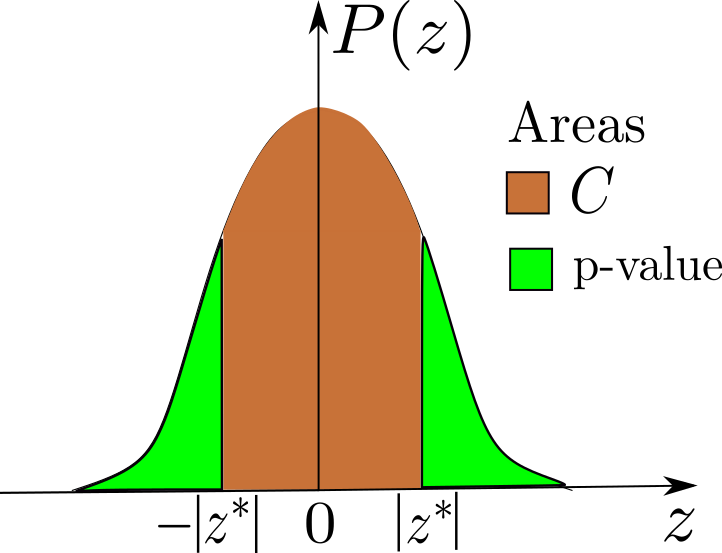
\includegraphics[width=2in]
{conventions/conf-int.png}
\caption{
Interpretation
of confidence level $C$
and p-value as areas under curve of the
Standard Normal Distribution (SND).}
\label{fig-conf-int}
\end{figure}

{\bf Confidence Level} $C$
and corresponding {\bf $|z^*|$ value}
(see Fig.\ref{fig-conf-int}):

\beq
C=\int_{-|z^*|}^{|z^*|} dz\;P(z) =
\Phi(|z^*|)-\Phi(-|z^*|)
=
2\left(\Phi(|z^*|)-\;\frac{1}{2}\right)
\label{eq-conf-level1}
\eeq
Equivalent definition:

\beq
C=P\left(
\underbrace{
\frac{|\rvx-\mu|}{\frac{\sigma}{\sqrt{n}}}
}_{|\rvz|}
<|z^*|\right)
\label{eq-conf-level2}
\eeq
For $C=95\%$,
$|z^*|=1.960\approx 2$.
For $C=99\%$, $|z^*|=2.576$.

Area of each tail
in Fig.\ref{fig-conf-int} is
usually called $\alpha$,
and the area of both tails is called
the {\bf p-value}:
\beq
C+\underbrace{2\alpha}_{p-value}=1
\;.
\eeq

Estimators\footnote{Don't
confuse the sample index $\s$
with the standard deviation $\s$.} of
mean $\mu$  and
standard deviation $\sigma$
from measurements $x^\s$
of a sub-population $\Sigma_1$ of
size $n=|\Sigma_1|$:
\beq
\HAT{\mu}=\ol{x}=\frac{1}{n}\sum_{\s \in\Sigma_1} x^\s
\eeq

\beq
\HAT{\s}^2=
\frac{1}{n-1}
\sum_{\s\in \Sigma_1} (x^\s-\ol{x})^2
\eeq


We get
from Eq.(\ref{eq-conf-level2}),
the {\bf Error bars (a.k.a. confidence intervals)}
and
{\bf Error $E$ (a.k.a. margin of error)}:



\beq
\text{ estimate of $x$
with error bars} =
\ol{x} \pm
\underbrace{
|z^*| \frac{\HAT{\s}}{\sqrt{n}}}_{E}
\label{eq-err-bars}
\eeq

\beq
n= \left(
\frac{|z^*|\HAT{\s}}{E}
\right)^2
\eeq

So far, we have assumed
that the sub-population (a.k.a. sample
population)
is normally distributed.
This might be false
for several reasons.
Some red flags: (1)
$n$ is too small (according to
a rule of thumb derived from
Central Limit Theorem, $n$
should be larger than 30
to insure a Normal Distribution).
(2) Sub-population not truly random
(i.i.d.)
because was taken
without replacement.
In many cases,
especially
when $n<30$,
the Student's t-distribution
models the sub-population statistics
much
better than the Normal distribution.


The {\rm Student's t-distribution } ${\rm Stud}(t;
\nu=n-1)$,
depends
on a parameter $\nu$
called the
number of
degrees of freedom.
In the case being considered here,
$\nu$ equals the
sub-population size $n$
minus one.
When fitting
the data with
Stud(), variable
$t$ replaces
variable $z$,
and ${\rm Stud}(t; \nu=n-1)$
replaces the Standard Normal distribution (SND)
$\caln(z; \mu=0, \sigma=1)$.
Stud() is symmetric about
the origin like SND,
but its tails
are fatter.
When fitting the data with Stud(),
the $|z^*|$
value is replaced
by a $|t^*|$ value.
Eq.(\ref{eq-conf-level1})
is replaced by


\beq
C=\int_{-|t^*|}^{|t^*|} dt\;{\rm Stud}(t) =
\Phi_S(|t^*|)-\Phi_S(-|t^*|)
=
2\left(\Phi_S(|t^*|)-\;\frac{1}{2}\right)
\label{eq-conf-level1-stu}
\;,
\eeq
where $\Phi_S()$
is the cumulative
distribution for  Stud().
Also, Eq.(\ref{eq-err-bars})
is replaced  by

\beq
\text{estimate of $x$
with error bars} =
\ol{x} \pm
\underbrace{
|t^*| \frac{\HAT{\s}}{\sqrt{n}}}_{E}
\;.
\eeq
Tables of $|t^*|(C,\nu=n-1)$
are available. Note
that $|t^*|$
depends on both $C$ and $\nu$,
whereas $|z^*|(C)$
depends only on $C$.

\section{p-value}


Given a parameter $\theta$, call
$\theta=\theta_0$ (or  $\theta<\theta_0$ or $\theta>\theta_0$) the
{\bf null hypothesis} $h_0$,
and call the negation of $h_0$ (i.e., 
$\theta\neq\theta_0$ (or  $\theta\geq\theta_0$ or $\theta\leq \theta_0$))
the {\bf alternative hypothesis} $h_1$.
Assume we
are given data $\vec{x}=\{x^\s|\s\in \Sigma\}$. Assume
also that we are given
distributions $P(\rvx=x|h)$ for $h\in \{h_0, h_1\}$,
and $P(\rvx=x)$. Now let

\beq
P(\vec{x}|h)=\prod_\s P(\rvx=x^\s|h)
\eeq


\beq
P(\vec{x})=\prod_\s P(\rvx=x^\s)
\eeq
(so the $x^\s$ are i.i.d.).

A Bayesian would assume that there
is a prior $P(h)$, and use it to
calculate
$P(h|\vec{x})=\frac{P(\vec{x}|h) P(h)}{P(\vec{x})}$.
$P(\rvh= h_0|\vec{x})$
is the probability that the null hypothesis is true.
A p-value is a monotonically increasing function of
$P(\rvh= h_0|\vec{x})$,
so Bayesians have no trouble saying
that  {\color{red} a p-value is
a measure of
$P(\rvh= h_0|\vec{x})$, i.e.,
a measure of the probability that
the null-hypothesis is true}.

Frequentists, on the other hand,
believe that $h$
is a ``parameter", not a random variable,
so  $P(\rvh= h_0|\vec{x})$
is undefined.
Next, we explain the correct
way of thinking about p-values, according to
Frequentists.
p-values were invented by Frequentists,
so it's worth hearing what they have to say
about them.
The Frequentist definition is not against Bayesianism,
and Bayesians, unlike Frequentists,
 don't accuse Frequentists of
having a sinfully incorrect
 definition of p-values. A Bayesian would just say:
our definition of p-values (shown
in red above) is not incorrect,
but the Frequentist definition is more precise than ours,
and doesn't assume a particular form for a prior.
We welcome it.

Call
the random variable
$\rvt$ the {\bf test statistic} and let 
$t^*$ be a user defined
parameter.
$\rvt$ and $t^*$
are defined so that
when $\rvt=t^*$,
the $h_0$ hypothesis is
on the threshold between 
being and not being satisfied.
Frequentists define the {\bf p-value} $p$ as

\beq
p=
\left\{
\begin{array}{ll}
P(\rvt \geq t^*|h_0)&\text{right-sided-tail,
if $h_0$ is $\theta<\theta_0$}
 \\
 P(\rvt\leq t^*|h_0)&\text{left-sided-tail,
 if $h_0$ is $\theta>\theta_0$}
 \\
 P(|\rvt| > |t^*|\;|h_0)&\text{double-sided-tail,
 if $h_0$ is $\theta=\theta_0$}
\end{array}
\right.
\eeq
Thus, for a Frequentist,
{\color{red} a p-value is a probabilistic
weight of the region
where the $h_0$ hypothesis is
defined (by the user) to be violated}.
If that weight is large,
then the region where
the $h_0$ hypothesis is
defined to be satisfied is small,
which means the $h_0$
hypothesis
is expected to be close to the truth.
The larger the p-value,
the closer $h_0$
is expected to be near the truth,
just like the Bayesian definition
says.
Note that the p-value
is a probability so it ranges in
value from 0 to 1.

Suppose we are given a subpopulation with $n$ samples,
 mean $\ol{x}$ and variance $\HAT{\s}$.
 Let $\theta_0=\mu_0$.
Define

\beq
\rvt=\rvz=
\frac{\rvx-\mu_0}{\frac{\HAT{\s}}{\sqrt{n}}}
\;. 
\eeq
For $n>30$, 

\begin{subequations}
\beqa
P(\rvz\geq z^*|h_0)
=1-\Phi(z^*)=\Phi(-z^*)
&\quad&\text{if $h_0$ is $\mu<\mu_0$}
\\
P(\rvz\leq z^*|h_0)=\Phi(z^*)
&\quad&\text{if $h_0$ is $\mu>\mu_0$}
\\
P(|\rvz|\geq |z^*|\;|h_0)=2\Phi(-|z^*|)
&\quad&\text{if $h_0$ is $\mu=\mu_0$}
\label{eq-double-tail}
\eeqa
\end{subequations}
where $\Phi(x)$ is the cumulative distribution
for the Standard Normal Distribution
$\caln(x;\mu=0, \s=0)$.
For $n<30$, $\Phi()$ is replaced
by $\Phi_S()$, where  $\Phi_S()$ is
the cumulative distribution
for the Student t-distribution ${\rm Stud}(x; \nu=n-1)$.
Note that Eq.(\ref{eq-double-tail})
agrees with
Eq.(\ref{eq-conf-level2}).

The quantity
\beq
z_{score}=
\frac{\ol{x}-\mu_0}{\frac{\HAT{\s}}{\sqrt{n}}}
\eeq
is called the {\bf z score}.
If $|z_{score}| > |z^*|$,
then the $h_0$ hypothesis
is defined to be violated
(for the double sided case).

\section{Short Summary of
Boolean Algebra}
See Ref.\cite{wiki-bool} for more info
about this topic.

Suppose $x, y, z\in \bool$. Define

\beq
x\text{ or }y=x\V y= x+y-xy
\;,
\eeq

\beq
x \text{ and }y=x\A y= xy
\;,
\eeq
and

\beq
\text{not }x=\ol{x}=1-x
\;,
\eeq
where we are using
normal addition and multiplication
on the right hand sides.\footnote{Note the
difference between $\V$ and modulus
2 addition $\oplus$.
For $\oplus$ (a.k.a. XOR): $x\oplus y=x+y-2xy$.}



\begin{table}[h!]
\centering
\begin{tabular}{|
>{\columncolor[HTML]{ECF4FF}}l |l|}
\hline
Associativity & \begin{tabular}[c]{@{}l@{}}$x \V (y \V z)=(x \V y) \V z$\\ $x \A (y \A z)=(x \A y) \A z$\end{tabular} \\ \hline
Commutativity & \begin{tabular}[c]{@{}l@{}}$x \V y=y \V x$\\ $x \A y=y \A x$\end{tabular} \\ \hline
Distributivity & \begin{tabular}[c]{@{}l@{}}$x \A (y \V z)=(x \A y) \V (x \A z)$\\ $x \V (y \A z)=(x \V y) \A (x \V z)$\end{tabular} \\ \hline
Identity & \begin{tabular}[c]{@{}l@{}}$x \V 0=x$\\ $x \A 1=x$\end{tabular} \\ \hline
Annihilator & \begin{tabular}[c]{@{}l@{}}$x \A 0=0$\\ $x \V 1= 1$\end{tabular} \\ \hline
Idempotence & \begin{tabular}[c]{@{}l@{}}$x \V x= x$\\ $x \A x= x$\end{tabular} \\ \hline
Absorption & \begin{tabular}[c]{@{}l@{}}$x \A (x \V y)= x$\\ $x \V (x \A y)= x$\end{tabular} \\ \hline
Complementation & \begin{tabular}[c]{@{}l@{}}$x \A \ol{x} = 0$\\ $x \V \ol{x}   = 1$\end{tabular} \\ \hline
Double negation & $\ol{(\ol{x})} = x$ \\ \hline
De Morgan Laws & \begin{tabular}[c]{@{}l@{}}$\ol{x} \A \ol{y} =\ol{(x \V y)}$\\ $\ol{x} \V \ol{y} = \ol{(x \A y)}$\end{tabular} \\ \hline
\end{tabular}
\caption{Boolean Algebra Identities}
\label{tab-bool-alg}
\end{table}

Actually, since
$x\A y=xy$, we can omit writing
the symbol $\A$. The symbol
$\A$ is useful to
exhibit the symmetry
of the identities, and
to remark
about
the analogous identities
for sets, where
$\A$ becomes intersection $\cap$
and $\V$ becomes union $\cup$. However,
for practical calculations,
$\A$ is an unnecessary nuisance.

Since $x\in \bool$,
\beq
P(\ol{x})=1-P(x)
\;.
\eeq

Clearly, from analyzing
the simple event space $(x,y)\in \bool^2$,
\beq
P(x\V y)= P(x) + P(y) - P(x\A y)
\;.
\eeq

\chapter{Navigating 
the ocean of Judea Pearl's Books}
%\addcontentsline{toc}{chapter}{Navigating the ocean of Judea Pearl's Books}

\label{ch0-nav-pearl}
Many
of the
greatest ideas 
in the bnet field 
were invented by Judea Pearl
and his collaborators.
Thus, this book is 
heavily indebted to
those great scientists.
Those ideas have had no clearer
and more generous 
expositor than Judea Pearl
himself.

Pearl has written
4 books that I have used
in writing Bayesuvius.
His 
1988 book Ref.\cite{pearl-1988book}
dates back to his pre-causal period.
That book I used to learn
about topics such as
d-separation, belief propagation,
Markov-blankets, and noisy-ORs.
3 other books that  he  wrote later,
in his causal period, 
are:
\begin{enumerate}
\item
In 2000 (1st ed.), and 2013 (2nd ed.),
Pearl published what
is so far
his most technical
and exhaustive book
on the subject of causality,
Ref.\cite{pearl-2013book}.
\item
In 2016,
he released 
together
with Glymour and Jewell,
a less advanced ``primer"
on causality, Ref.\cite{pearl-primer}.
\item
In 2018, 
he released 
together with
Mackenzie his
lovely  ``The Book of Why",
 Ref.\cite{book-why}.
\end{enumerate}
Those 3 books I used to learn
about causality topics
such as Do Calculus,
backdoor and frontdoor
adjustment formulae,
linear 
deterministic 
bnets with exogenous noise,
and counterfactuals.

A micro poem written by me
to celebrate Judea Pearl and 
his work:
 
\section*{I, Robot}
\begin{verse}
Let other robots {\tt talk()},\\
while I,\\
{\tt talk()}, {\tt do()} and {\tt imagine()}.
\end{verse}

\chapter{ARACNE: COMING SOON}
\label{ch-aracne}

A generalization
of Chow-Liu trees
that is able to learn 
polytrees. Implemented 
in \bnlearn Ref.\cite{bnlearn}

This chapter
is based on
Ref.\cite{aracne}




\chapter{Backdoor Adjustment}
\label{chap-bdoor}

The backdoor (BD) adjustment
theorem is proven in 
Chapter \ref{chap-do-calc}
from the rules of do-calculus.
The goal 
of this chapter is
to give examples
of the use of that
theorem.
We will restate
the theorem in this chapter,
sans proof.
There is no need
to understand the
theorem's
proof in order to use it.
However, you
will
need to skim Chapter \ref{chap-do-calc}
in order to familiarize 
yourself with
the notation used to state the 
theorem.
This chapter also assumes
that you are comfortable 
with the  rules 
for checking for d-separation. Those rules
are covered in Chapter \ref{chap-dsep}.



\bdoordef
\begin{claim} {\bf Backdoor Adjustment
 Theorem}

\bdoorclaim
\end{claim}
\proof 
See Chapter \ref{chap-do-calc}
\qed

Examples:
\begin{enumerate}
\hrule\item
\beq
\xymatrix{
&\rvz\ar[dr]
\\
\rvx\ar[rr]\ar[ru]&&\rvy
}
\eeq

BD criterion satisfied if
$\rvx.=\rvx, \rvy.=\rvy, \rvz.=\emptyset$.
 No adjustment necessary.

\beq
P(y|\rho \rvx=x)=P(y|x)
\eeq

\hrule\item
\beq
\xymatrix{
&\rvz\ar[dl]\ar[dr]
\\
\rvx\ar[rr]&&\rvy
}
\eeq
BD criterion satisfied if
$\rvx.=\rvx, \rvy.=\rvy, \rvz.=\rvz$.

Note that 
here the backdoor formula adjusts
the parents  of $\rvx.$.

\hrule\item
\beq
\xymatrix{
&\rvz\ar[dl]\ar[dr]
\\
\rvx\ar[r]&\rvm\ar[r]&\rvy
}
\eeq
BD criterion satisfied if
$\rvx.=\rvx, \rvy.=\rvy, \rvz.=\rvz$.

\hrule\item
\beq
\xymatrix{
&*+[F]{\rvz}\ar[dl]\ar[dr]
\\
\rvx\ar[r]&\rvm\ar[r]&\rvy
}
\eeq
BD criterion is
impossible to satisfy if
$\rvx.=\rvx, \rvy.=\rvy$.
However, the front-door criterion can be
satisfied. See Chapter
\ref{chap-fdoor}.

\hrule\item
\beq
\xymatrix{
*+[F]{\rvw}\ar[d]\ar[r]
&\rvz\ar[d]
\\
\rvx\ar[r]&\rvy
}
\eeq

BD criterion satisfied if
$\rvx.=\rvx, \rvy.=\rvy, \rvz.=\rvz$.
Note that 
here the backdoor formula cannot
adjust the single parent $\rvw$
of $\rvx$ because it is hidden, 
but we are able to 
block the backdoor path 
by conditioning on $\rvz$ 
instead.


\hrule\item
\beq
\xymatrix{
*+[F]{\rve}\ar[d]\ar[r]
&\rvz\ar[dl]\ar[dr]
&\rva\ar[d]\ar[l]
\\
\rvx\ar[rr]&&\rvy
}
\eeq

Conditioning
on $\rvz$
blocks 
backdoor path
$\rvx-\rvz-\rvy$, 
but 
opens path $\rvx-\rve-\rvz-\rva-\rvy$
because $\rvz$ is a collider
for that path. That
path is blocked
if we also
condition on $\rva$, 
which is possible
because $\rva$ is
observed.
In conclusion,
the BD criterion is satisfied if
$\rvx.=\rvx$, 
$\rvy.=\rvy$
and 
$\rvz.=(\rvz, \rva)$.

Conditioning on 
the parents of 
$\rvx.$
is often
enough
to block
all
backdoor paths.
However, sometimes
some of the 
parents are unobserved 
and one must 
condition on other
nodes that
are not parents of $\rvx.$
in order to satisfy
the BD criterion. 


\hrule\item
\beq
\xymatrix{
\rvz\ar[d]&&\rvt\ar[ll]\ar[d]
\\
\rvw&\rvx\ar[r]\ar[l]&\rvy
}
\eeq

No need to control
anything 
because only possible
backdoor path is blocked by collider $\rvw$.
Hence,

\beq
P(y|\rho\rvx=x)=P(y|x)
\;.
\eeq

However, 
if for some reason 
we want to control
$\rvt$, we
can do so. We  can't
control
$\rvw$ though, 
because $\rvw\in de(\rvx)$.
Thus, the
BD criterion is
satisfied if
 $\rvx.=\rvx$,
$\rvy.=\rvy$ and 
$\rvz.=\rvt$.
Therefore, 

\beq
P(y|\rho \rvx=x)=
\sum_{t} P(y|x, t)P(t)
\label{eq-bdoor-t-sum}
\;.
\eeq


\hrule
\item
Discuss reasons why 
multiple possible sets $\rvz.$
that satisfy the BD criterion
can be advantageous.
\begin{itemize}
\item
Can evaluate $P(y.|\rho \rvx.=x.)$
multiple ways and compare the results.
This is a test that the causal bnet 
is correct.
\item
It might 
be easier or 
less expensive to get data for
some $\rvz.$ 
more than for others.
\end{itemize}

\hrule
\item (Taken from online course notes 
Ref.\cite{ethz-causality})

Consider the bnet

\beq
\xymatrix{
\rvx_2\ar[d]\ar[r]
&\rvx_3&
\rvx_4\ar[d]\ar[l]
\\
\rvx_1\ar[d]\ar[r]
&\rvx_6\ar[d]\ar[r]
&\rvx_5\ar[d]
&\rvx_7\ar[l]
\\
\rvx_8&\rvx_9&\rvx_{10}
}
\eeq
If $\rvx.=\rvx_1$ and 
$\rvy.=\rvx_5$, find
all possible 
adjustment multinodes $\rvz.$ that 
satisfy the BD criterion.
Ans:
\begin{multicols}{4}
\begin{itemize}
\item $ \emptyset$
\item $\rvx_2$
\item $\rvx_4$
\item $\rvx_2, \rvx_4$
\item $\rvx_2,\rvx_3$
\item $\rvx_3, \rvx_4$
\item $\rvx_2, \rvx_3, \rvx_4$
\end{itemize}
\end{multicols}
Add $\rvx_7$
to each of the previous 7 possible
$\rvz.$. This gives
 a total of 14 possible 
adjustment multinodes $\rvz.$. 


  



\end{enumerate}
\chapter{Back Propagation
 (Automatic Differentiation)}

\section{General Theory}

\subsection{Jacobians}

Suppose
 $f:\RR^{nx}\rarrow \RR^{nf}$
and 

\beq
y=f(x)
\;.
\eeq
Then the Jacobian $\pder{y}{x}$
is defined as the matrix with entries\footnote{
Mnemonic for remembering 
order of indices: $i$ in numerator/$j$ in denominator
becomes index $i/j$ of Jacobian matrix.}

\beq
\left[\pder{y}{x}\right]_{i,j}=
\pder{y_i}{x_j}
\;.
\eeq




Jacobian of function composition.
Supoose $f:\RR^{nx}\rarrow\RR^{nf}$,
$g:\RR^{nf}\rarrow \RR^{ng}$. If

\beq
y=g\circ f (x)
\;,
\eeq
then

\beq
\pder{y}{x}
=
\pder{g}{f}
\pder{f}{x}
\;.
\eeq
Right hand side
of last equation 
is a product
of two matrices
so order of matrices is important.

\subsection{
bnets for function
composition, 
forward propagation and back propagation}



\begin{figure}[h!]
\centering
$$
\xymatrix{
\rvf^4
&
\rvf^3\ar[l]
&
\rvf^2\ar[l]
&
\rvf^1\ar[l]
&
\rvf^0\ar[l]
\\
&&\text{$(a)$ Composition}
\\
\ul{\pder{f^4}{x}}
&
\ul{\pder{f^3}{x}}\ar[l]
&
\ul{\pder{f^2}{x}}\ar[l]
&
\ul{\pder{f^1}{x}}\ar[l]
&
\ul{1}\ar[l]
\\
&&\text{$(b)$ Forward-p}
\\
\ul{1}\ar[r]
&
\ul{\pder{y}{f^3}}\ar[r]
&
\ul{\pder{y}{f^2}}\ar[r]
&
\ul{\pder{y}{f^1}}\ar[r]
&
\ul{\pder{y}{f^0}}
\\
&&\text{$(c)$ Back-p}
}
$$
\caption{bnets for function
composition,
forward propagation and back propagation
for $nf=5$ nodes.}
\label{fig-backp-abc}
\end{figure}


Let
\beq
y=f^4\circ f^3 \circ f^2 \circ f^1 (x)
\;.
\eeq
This function composition chain can be
represented by the bnet
Fig.\ref{fig-backp-abc}$(a)$
with TPMs

\beq\color{blue}
P(f^\mu|f^{\mu-1})=
\indi(f^\mu=f^\mu(f^{\mu-1}))
\;
\eeq
for $\mu=1, 2,3,4$.


Note that
\beqa
\pder{y}{x}&=&
\pder{y}{f^3}
\pder{f^3}{f^2}
\left[
\pder{f^2}{f^1}
\pder{f^1}{x}
\right]
\\
&=&
\pder{y}{f^3}
\left[
\pder{f^3}{f^2}
\pder{f^2}{x}
\right]
\\
&=&
\left[
\pder{y}{f^3}
\pder{f^3}{x}
\right]
\\
&=&
\pder{y}{x}
\;.
\eeqa
This forward propagation can be
represented by the bnet
Fig.\ref{fig-backp-abc}$(b)$
with node TPMs

\beq\color{blue}
P(\pder{f^{\mu+1}}{x}\cond
 \pder{f^{\mu}}{x})=
\indi(\pder{f^{\mu+1}}{x}=
\pder{f^{\mu+1}}{f^{\mu}}
\pder{f^{\mu}}{x} 
)\;
\eeq
for $\mu=1,2,3$.

Note that

\beqa
\pder{y}{x}&=&
\left[
\pder{y}{f^3}
\pder{f^3}{f^2}
\right]
\pder{f^2}{f^1}
\pder{f^1}{x}
\\
&=&
\left[
\pder{y}{f^2}
\pder{f^2}{f^1}
\right]
\pder{f^1}{x}
\\
&=&
\left[
\pder{y}{f^1}
\pder{f^1}{x}
\right]
\\
&=&
\pder{y}{x}\;.
\eeqa
This back propagation can be
represented by the bnet
Fig.\ref{fig-backp-abc}$(c)$
with node TPMs

\beq\color{blue}
P(
\pder{y}{f^{\mu}}
\cond 
\pder{y}{f^{\mu+1}}
)=
\indi(
\pder{y}{f^{\mu}}
=
\pder{y}{f^{\mu+1}}
\pder{f^{\mu+1}}{f^{\mu}}) 
\;
\eeq
for $\mu=2,1,0$.

$\pder{f^{\mu+1}}{f^{\mu}}$
is a Jacobian matrix
so the order of multiplication
matters. In forward prop,
it pre-multiplies,
and in back prop it post-multiplies.

\section{Application to Neural Networks}

\subsection{Absorbing $b^\lam_i$ into $w_{i|j}$.}

\begin{figure}[h!]
$$\xymatrix
{
\rvx\ar[r]\ar[rd]
&\rvh^0_2\ar[r]\ar[rd]
&\rvh^1_2\ar[r]\ar[rd] 
& Y_2
\\
& \rvh^0_1 \ar[r]\ar[ru]
&\rvh^1_1 \ar[r]\ar[ru]
& Y_1
\\
& \rvh^0_0 \ar[u]\ar@/^1pc/[uu]
&\rvh^1_0\ar[u]\ar@/^1pc/[uu]
& \rvY_0\ar[u]\ar@/^1pc/[uu]
}$$
\caption{Nodes $\rvh^0_0, \rvh^1_0, \rvY_0$
are all set to 1. They
allow us to absorb $b^\lam_i$
into the first column of
$w^\lam_{i|j}$.}
\label{fig-backp-abs}
\end{figure}

Below are, printed 
in blue, the TPMs
for the nodes of a NN bnet,
as given in Chapter \ref{ch-nn}.

For all hidden layers $\lam=0, 1, \dots,
\Lambda-2$,

\beq\color{blue}
P(h^{\lam}_i\cond h^{\lam-1}_.)=
\delta\left(h^{\lam}_i,
\cala_i^\lam(\sum_j
 w^{\lam}_{i|j}
h^{\lam-1}_j + b^{\lam}_i)\right)
\eeq
for $i=0, 1, \ldots, nh(\lam)-1$.
For the output visible layer $\lam=\Lambda-1$:

\beq\color{blue}
P(Y_i\cond h^{\Lambda-2}_.)=
\delta \left(Y_i,
\cala_i^{\Lambda-1}(\sum_j w^{\Lambda-1}_{i|j}
h^{\Lambda-2}_j + b^{\Lambda-1}_i)\right)
\;
\eeq
for $i=0, 1, \ldots, ny-1$.


For each $\lam$, replace the matrix
 $w^\lam_{\cdot|\cdot}$ 
by 
the augmented matrix
$[b^\lam., w^\lam_{\cdot|\cdot}]$
so that the new
 $w^\lam_{\cdot|\cdot}$ satisfies

\beq
w^{\lam}_{i|0}=b_i^{\lam}
\;
\eeq

Let the nodes $\rvh_0^\lam$
for all $\lam$ and $\rvY_0$ be
root nodes (so no arrows 
pointing into them).
For each $\lam$, draw arrows from 
$\rvh_0^\lam$ to all other nodes 
in that same layer.
Draw arrows from 
$\rvY_0$ to all other nodes 
in that same layer.

After performing the
above steps,
the TPMs,
printed in blue,
for the nodes of the NN bnet
 are as follows:

For all hidden layers $\lam=0, 1, \dots,
\Lambda-2$,

\beq\color{blue}
P(h^\lam_0)=\delta(h^\lam_0,1)
\;,
\eeq
and

\beq\color{blue}
P(h^{\lam}_i\cond h^{\lam-1}_., h_0^\lam=1)=
\delta\left(h^{\lam}_i,
\cala_i^\lam(\sum_{j}
 w^{\lam}_{i|j}
h^{\lam-1}_j)\right)
\eeq
for $i=1, \ldots, nh(\lam)-1$.
For the output visible layer $\lam=\Lambda-1$:

\beq\color{blue}
P(Y_0)=\delta(Y_0,1)
\;,
\eeq
and

\beq\color{blue}
P(Y_i\cond h^{\Lambda-2}_., Y_0=1)=
\delta \left(Y_i,
\cala_i^{\Lambda-1}(\sum_j w^{\Lambda-1}_{i|j}
h^{\Lambda-2}_j)\right)
\;
\eeq
for $i=1, 2, \ldots, ny-1$.

\subsection{
bnets for function
composition, 
forward propagation and back propagation
for NN}

\begin{figure}[h!]
\centering
$$
\xymatrix{
\ul{\cala^3}
&
\ul{\calb^3}\ar[l]
&
\ul{\cala^2}\ar[l]
&
\ul{\calb^2}\ar[l]
&
\ul{\cala^1}\ar[l]
&
\ul{\calb^1}\ar[l]
&
\ul{\cala^0}\ar[l]
&
\ul{\calb^0}\ar[l]
&
\rvx\ar[l]
\\
&&\text{$(a)$}
\\
\ul{\pder{\cala^3}{x}}
&
\ul{\pder{\calb^3}{x}}\ar[l]
&
\ul{\pder{\cala^2}{x}}\ar[l]
&
\ul{\pder{\calb^2}{x}}\ar[l]
&
\ul{\pder{\cala^1}{x}}\ar[l]
&
\ul{\pder{\calb^1}{x}}\ar[l]
&
\ul{\pder{\cala^0}{x}}\ar[l]
&
\ul{\pder{\calb^0}{x}}\ar[l]
&
\ul{1}\ar[l]
\\
&&\text{$(b)$}
\\
\ul{1}\ar[r]
&
\ul{\pder{Y}{\calb^3}}\ar[r]
&
\ul{\pder{Y}{\cala^2}}\ar[r]
&
\ul{\pder{Y}{\calb^2}}\ar[r]
&
\ul{\pder{Y}{\cala^1}}\ar[r]
&
\ul{\pder{Y}{\calb^1}}\ar[r]
&
\ul{\pder{Y}{\cala^0}}\ar[r]
&
\ul{\pder{Y}{\calb^0}}\ar[r]
&
\ul{\pder{Y}{x}}
\\
&&\text{$(c)$}
}
$$
\caption{bnets for $(a)$ function
composition, $(b)$
forward propagation and $(c)$ back propagation
for a neural net with 4 layers (3 hidden and
output visible).}
\label{fig-backp-nn}
\end{figure}
.\\
From here on, we will rename $y$ above
by $Y=\hat{y}$ and 
consider samples $y[i]$ for 
$i=0, 1, \ldots, nsam-1$.
The Error (aka loss or cost function) is

\beq
\cale =\frac{1}{nsam}
\sum_{\sigma=0}^{nsam-1}\sum_{i=0}^{ny-1}
|Y_i-y_i[\sigma]|^2
\eeq
To perform simple gradient descent,
one uses:

\beq
(w_{i|j}^\lam)'=w_{i|j}^\lam
-\eta\pder{\cale}{w^\lam_{i|j}}
\;.
\eeq
One has

\beq
\pder{\cale}{w^\lam_{i|j}}=
\frac{1}{nsam}
\sum_{\sigma=0}^{nsam-1}\sum_{i=0}^{ny-1}
2(Y_i-y_i[\sigma])\pder{Y}{w^\lam_{i|j}}
\;.
\eeq
Define $\calb^\lam_i$ thus


\beq
\calb^\lam_i(h^{\lam-1})=
\sum_j w^{\lam}_{i|j}h^{\lam-1}_j
\;.
\label{eq-calb}
\eeq
Then

\beqa
\pder{Y}{w^\lam_{i|j}}&=&
\pder{Y}{\calb^\lam_i}
\pder{\calb_i^\lam}{w^\lam_{i|j}}
\\
&=&\pder{Y}{\calb^\lam_i}
h^{\lam-1}_j
\eeqa

\beqa
\pder{\cale}{w^\lam_{i|j}}&=&
\pder{\cale}{\calb^\lam_j}
\pder{\calb^\lam_j}{w^\lam_{i|j}}
\\
&=&
\pder{\cale}{\calb^\lam_j}
h^{\lam-1}_j
\;.
\eeqa
This suggest that
we can calculate 
the derivatives of the error
$\cale$
with respect to the weights
$w^\lam_{i|j}$ in two 
stages, using an intermediate 
quantity $\delta^\lam_j$:

\beq
\left\{
\begin{array}{l}
\delta^\lam_j=\pder{\cale}{\calb^\lam_j}
\\
\pder{\cale}{w^\lam_{i|j}}=\delta^\lam_j h^{\lam-1}_j
\end{array}
\right.
\eeq

To 
apply what we learned in the earlier
General Theory
section of this chapter, 
consider a NN with 4
layers (3 hidden, and the
output visible one). Define the
functions $f_i$
as follows:


\beq
f^0_i=x_i
\eeq

\beqa
\text{Layer 0:}&
f^1_i=\calb_i^0(x_i),&
f^2_i=\cala_i^0(\calb_i^0)
\\
\text{Layer 1:}&
f^3_i=\calb_i^1(\cala_i^0),&
f^4_i=\cala_i^1(\calb_i^1)
\\
\text{Layer 2:}&
f^5_i=\calb_i^2(\cala_i^1),&
f^6_i=\cala_i^2(\calb_i^2)
\\
\text{Layer 3:}&
f^7_i=\calb_i^3(\cala_i^2),&
f^8_i=\cala_i^3(\calb_i^3)
\eeqa




%\beq\color{blue}
%P(\cala^\lam|\cala^{\lam-1})=
%\indi(\cala^\lam=\cala^\lam\circ\calb^\lam(\cala^{\lam-1}))
%\;
%\eeq

%\beq\color{blue}
%P(\pder{\cala^{\lam+1}}{x}\cond
%\pder{\cala^{\lam}}{x})=
%\indi(\pder{\cala^{\lam+1}}{x}=
%\pder{\cala^{\lam+1}}{\calb^{\lam+1}}
%\pder{\calb^{\lam+1}}{\cala^{\lam}}
%\pder{\cala^{\lam}}{x} 
%)\;
%\eeq

See Fig.\ref{fig-backp-nn}. The
TPMs, printed in blue,
for the nodes
of  the bnet $(c)$
for back propagation, are:

\beq\color{blue}
P(
\pder{Y}{\calb^{\lam}}
\cond 
\pder{Y}{\calb^{\lam+1}}
)=
\indi(
\pder{Y}{\calb^{\lam}}
=
\pder{Y}{\calb^{\lam+1}}
\pder{\calb^{\lam+1}}{\cala^{\lam}}
\pder{\cala^{\lam}}{\calb^{\lam}}) 
\;.
\label{eq-backp-nn-1}
\eeq
One has

\beq
\pder{\cala^{\lam}_i}{\calb^{\lam}_j}
=
D{\cala_i}^\lam(\calb_i^\lam)\delta(i,j)
\eeq
where $D{\cala}^\lam_i(z)$
is the derivative of 
$\cala^\lam_i(z)$.

From Eq.(\ref{eq-calb})

\beq
\calb^{\lam+1}_i(\cala^{\lam})=
\sum_j w^{\lam+1}_{i|j}\cala^{\lam}_j
\eeq
so

\beq
\pder{\calb_i^{\lam+1}}{\cala_j^{\lam}}
=w^{\lam+1}_{i|j}
\;.
\eeq
Therefore, Eq.(\ref{eq-backp-nn-1})
implies

\beq\color{blue}
P(
\pder{Y}{\calb^{\lam}_j}
\cond 
\pder{Y}{\calb^{\lam+1}_j}
)=
\indi(
\pder{Y}{\calb^{\lam}_j}
=
\sum_i
\pder{Y}{\calb_i^{\lam+1}}
D{\cala}^\lam_j(\calb^\lam_j)
w^{\lam+1}_{i|j}
) 
\;,
\eeq

\beq\color{blue}
P(
\pder{\cale}{\calb^{\lam}_j}
\cond 
\pder{\cale}{\calb^{\lam+1}_j}
)=
\indi(
\pder{\cale}{\calb^{\lam}_j}
=
\sum_i
\pder{\cale}{\calb_i^{\lam+1}}
D{\cala}^\lam_j(\calb^\lam_j)
w^{\lam+1}_{i|j}
) 
\;,
\eeq

\beq\color{blue}
\boxed{
P(
\delta^{\lam}_j
\cond 
\delta^{\lam+1}_j
)=
\indi(
\delta^{\lam}_j
=
\sum_i
\delta_i^{\lam+1}
D{\cala}^\lam_j(\calb^\lam_j))
w^{\lam+1}_{i|j}
)
}
\;.
\eeq

First delta of iteration, belonging to output 
layer $\lam=\Lambda-1$:

\beqa
\delta^{\Lambda-1}_j&=&
\pder{\cale}{\calb^{\Lambda-1}_j}
\\
&=&
\frac{1}{nsam}
\sum_{\sigma=0}^{nsam-1}\sum_{i=0}^{ny-1}
2(Y_i-y_i[\sigma])
D{\cala}^{\Lambda-1}_i(\calb^{\Lambda-1}_i)\delta(i,j)
\\
&=&
\frac{1}{nsam}
\sum_{\sigma=0}^{nsam-1}
2(Y_j-y_j[\sigma])
D{\cala}^{\Lambda-1}_j(\calb^{\Lambda-1}_j)
\eeqa

Cute expression for 
derivative of sigmoid function:
\beq
D\smoid(x)=
\smoid (x)(1-\smoid(x))
\eeq

\section{General bnets instead of Markov chains
induced by layered structure of NNs}

\beq
P(
\delta_\rvx
\cond 
(\delta_\rva)_{\rva\in ch(\rvx)}
)=
\indi(
\delta_\rvx
=
\sum_{\rva\in ch(\rvx)}
\delta_\rva
D{\cala}_\rvx(\calb_\rvx))
w_{\rva|\rvx}
)
\;
\eeq

Reverse arrows of original bnet
and define the TPM
of nodes of ``time reversed" bnet by

\beq\color{blue}
\boxed{
P(
\delta_\rvx
\cond 
(\delta_\rva)_{\rva\in pa(\rvx)}
)=
\indi(
\delta_\rvx
=
\sum_{\rva\in pa(\rvx)}
\delta_\rva
D{\cala}_\rvx(\calb_\rvx))
w^T_{\rvx|\rva}
)
}
\;
\eeq


\chapter{Basic Curve Fitting
Using Gradient Descent}
\label{ch-basic-fit}

\begin{figure}[h!]
\centering
$$\xymatrix{
&\vec{\rvx}\ar[d]\ar[r]&\ul{\vecy}
\ar[d]&\\
\phi\ar[r]\ar@/_1pc/[rrr]&
\vec{\hat{\rvy}}\ar[r]&\cale\ar[r]&\phi'
}$$
\caption{Basic curve fitting bnet.}
\label{fig-bfit}
\end{figure}


Samples 
$(x[i], y[i])\in S_\rvx\times S_\rvy$
are given. $nsam(\vecx)=nsam(\vecy)$.

Estimator function 
$\hat{y}(x; \phi)$
for $x\in S_\rvx$ and $\phi\in\RR$
is given.

Let 
\beq
P_{\rvx, \rvy}(x,y)=
\frac{1}{nsam(\vecx)}
\sum_i \indi(x=x[i], y=y[i])
\;.
\eeq


Let 
\beq
\cale(\vecx, \vecy, \phi)=
\frac{1}{nsam(\vec{y})}
\sum_i
|y[i]-\hat{y}(x[i]; \phi)|^2
\;
\eeq
$\cale$ is called the mean square error.

Best fit is parameters $\phi^*$
such that

\beq 
\phi^*= \argmin_\phi
\cale(\vecx, \vecy, \phi)
\;.
\eeq

The node TPMs for
the basic curve fitting bnet
 Fig.\ref{fig-bfit} are
printed below in blue.

\beq\color{blue}
P(\phi) \text{ = given}
\;.
\eeq
The first time
it is used, $\phi$ is arbitrary.
After the first time, it is determined 
by previous stage.

\beq\color{blue}
P(\vecx)=\prod_i P_\rvx(x[i])
\eeq

\beq\color{blue}
P(\vecy|\vecx)=\prod_i P_{\rvy|\rvx}(y[i]\cond x[i])
\eeq

\beq\color{blue}
P(\hat{y}[i]|\phi, \vecx)=
\delta(\hat{y}[i], \hat{y}(x[i];\phi))
\eeq


\beq\color{blue}
P(\cale|\vec{\hat{y}}, \vecy)=
\delta(\cale,\frac{1}{nsam(\vecx)}
\sum_i |y[i]-\hat{y}[i]|^2)
\;.
\eeq


\beq\color{blue}
P(\phi'|\phi, \cale)=
\delta(\phi',
\phi-\eta\partial_\phi\cale)
\eeq
$\eta>0$ is the descent rate.
If $\Delta \phi=\phi'-\phi=-\eta 
\frac{\partial\cale}
{\partial \phi}$, then
 $\Delta \cale=\frac{-1}{\eta}
(\Delta\phi)^2<0$  so this will
minimize the error
$\cale$.
This is called ``gradient descent".
\chapter{Bell  
and Clauser-Horne Inequalities 
in Quantum Mechanics}

\begin{figure}[h!]
\centering
$$\xymatrix{
&\ul{\lambda}\ar[dr]\ar[dl]&\\
\ul{x_1^{\alpha_1}}&&\ul{x_2^{\alpha_2}}
}$$
\caption{bnet used to discuss Bell 
and Clauser-Horne inequalities 
in Quantum Mechanics.}
\label{fig-bell}
\end{figure}

I wrote an article about
this in 2008 for
my blog \qt{Quantum Bayesian Networks}.
See Ref.\cite{bell-blog}.
\chapter{Binary Decision Diagrams}\label{ch-binarydd}

\begin{figure}[h!]
$$
\begin{array}{c}
\xymatrix@C=.1pc{
&&&&&&&\stackrel{\rvA}{x_1?}\ar@{-->}[dllll]
\ar[drrrr]
\\
&&&\stackrel{\rvA_0}{x_2?}\ar@{-->}[dll]\ar[drr]
&&&&&&&&\stackrel{\rvA_1} {x_2?}\ar@{-->}[dll]\ar[drr]
\\
&\stackrel{\rvA_{00}}{ x_3?}\ar@{-->}[dl]\ar[dr]
&&&&\stackrel{\rvA_{01}} {x_3?}\ar@{-->}[dl]\ar[dr]
&&&&\stackrel{\rvA_{10}}{ x_3?}\ar@{-->}[dl]\ar[dr]
&&&&\stackrel{\rvA_{11}}{x_3?}\ar@{-->}[dl]\ar[dr]
\\
\rvA_{000}\ar[d]
&&\rvA_{001}\ar[d]
&&\rvA_{010}\ar[d]
&&\rvA_{011}\ar[d]
&&\rvA_{100}\ar[d]
&&\rvA_{101}\ar[d]
&&\rvA_{110}\ar[d]
&&\rvA_{111}\ar[d]
\\
\Rect{1}
&&\Rect{0}
&&\Rect{0}
&&\Rect{1}
&&\Rect{0}
&&\Rect{0}
&&\Rect{1}
&&\Rect{1}
}
\\
\begin{array}{ccc|l}
x_1&x_2&x_3&f(A_{x_1,x_2,x_2})
\\ \hline\hline
0
&0
&0
&1
\\ \hline
0
&0
&1
&0
\\ \hline
0
&1
&0
&0
\\ \hline
0
&1
&1
&1
\\ \hline
1
&0
&0
&0
\\ \hline
1
&0
&1
&0
\\ \hline
1
&1
&0
&1
\\ \hline
1
&1
&1
&1
\\ \hline
\end{array}
\end{array}
$$
\caption{Example of a binary tree and its truth table.
The truth table gives the values of $
f(x_1, x_2,x_3)=
\bar{x}_1(x_2+\bar{x}_3)  + x_1 x_2 $ }
\label{fig-bdd-tree}
\end{figure}

This chapter is based
on Wikipedia article Ref.\cite{wiki-bdd}
and other references.

A {\bf Binary Decision Diagram} (BDD) is a 
graph which represents 
in a more concise manner
the information in
a binary tree and
its accompanying truth table.

Fig.\ref{fig-bdd-tree} shows an
example of a binary tree and its 
truth table.
We will  convert this tree 
 into a BDD in this chapter. Each node asks a question with a binary (Boolean) answer. An answer of 0 (resp., 1 ) is indicated by a dashed (resp., full) arrow. The same question is asked by all nodes at the same level (i.e., depth) of the tree. In addition to the question, nodes are labeled uniquely by the random variable $\rvA_{x_1, x_2, \ldots, x_n}$,
where $n$ is the level of the node
and $x_i$ is the answer to the question $x_i?$.
The leaves of
the tree are square boxes that report 

\beq
f(x_1, x_2,x_3)=
\bar{x}_1(x_2+\bar{x}_3)  + x_1 x_2
\label{eq-bdd-truth-table}
\eeq
\begin{figure}[h!]
$$
\xymatrix@C=.1pc{
&&&&&&&x_1?\ar@{-->}[dllll]
\ar[drrrr]
\\
&&&x_2?\ar@{-->}[dll]\ar[drr]
&&&&&&&&x_2?\ar@{-->}[dll]\ar[drr]
\\
&x_3?\ar@{-->}[dl]\ar[dr]
&&&&x_3?\ar@{-->}[dl]\ar[dr]
&&&&x_3?\ar@{-->}[dl]\ar[dr]
&&&&x_3?\ar@{-->}[dl]\ar[dr]
\\
\Rect{1}
&&\Rect{0}
&&\Rect{0}
&&\Rect{1}
&&\Rect{0}
&&\Rect{0}
&&\Rect{1}
&&\Rect{1}
}
$$
\caption{The same tree as in Fig.\ref{fig-bdd-tree}, after dropping 
some labels that are not needed
for our discussion of BDDs.}
\label{fig-bdd-tree-simp}
\end{figure}


Fig.\ref{fig-bdd-tree-simp} shows
the same tree as in  Fig.\ref{fig-bdd-tree}, after dropping 
some labels that are not needed
for our discussion of BDDs.
Note that the {\bf question ordering} of the tree is
$x_1<x_2<x_3$. Other question
orderings such as $x_2< x_1 < x_3$
are possible. For a given
truth table, some question 
orderings lead to a BDD 
that has the full  
exponential complexity $2^n$
of the tree, where $n$ is 
the number of levels. Other question orderings
might lead to BDDs that have lower (such as linear in $n$) 
complexity.



\subsection{Conversion of Binary Tree into BDD}

A BDD is obtained
from a binary tree by 
successive application of the
following
3 rules:

\begin{enumerate}
\item Merge equivalent leaves (EL)
\item Merge isomorphic nodes (IN)
\item Eliminate parallel 0/1 arrows (PA) by merging source
and target nodes of the parallel  arrows.
\end{enumerate}

Fig.\ref{fig-el-pa-example} 
gives an example
of the application of rules EL and PA.
Fig.\ref{fig-example-in-rule}
gives an example of the 
application of the IN rule.


\begin{figure}[h!]
$$
\xymatrix{
\\\\
\stackrel{EL}{\implies}}
\xymatrix@C=.1pc{
&&&&&&&x_1?\ar@{-->}[dllll]
\ar[drrrr]
\\
&&&x_2?\ar@{-->}[dll]\ar[drr]
&&&&&&&&x_2?\ar@{-->}[dll]\ar[drr]
\\
&x_3?\ar@{-->}[drrrrrrr]\ar[drrrrr]
&&&&x_3?\ar@{-->}[dr]\ar[drrr]
&&&&x_3?\ar@{-->}[dlll]\ar@/_1pc/[dlll]
&&&&x_3?\ar@{-->}[dlllll]\ar@/_1pc/[dlllll]
\\
&&
&&
&&\Rect{0}
&&\Rect{1}
&&
&&
&&
}
\xymatrix{
\\\\\stackrel{PA}{\implies}}
\xymatrix@C=.1pc{
&&&&&&x_1?\ar@{-->}[dllll]
\ar[d]
\\
&&x_2?\ar@{-->}[dll]\ar[drr]
&&&&x_2?\ar@{-->}[ddll]\ar[dd]
\\
x_3?\ar@{-->}[drrrrrr]\ar[drrrr]
&&&&x_3?\ar@{-->}[d]\ar[drr]
\\
&&
&&\Rect{0}
&&\Rect{1}
&&
&&
&&
}
$$
\caption{This is the 
result of applying the
the EL rule, followed by the PA
rule, to Fig.\ref{fig-bdd-tree-simp}.}
\label{fig-el-pa-example}
\end{figure}

\begin{figure}[h!]
$$
\begin{array}{c}
\xymatrix@C=.1pc{
&&&&&&x_1?\ar@{-->}[dllll]
\ar[drrr]
\\
&&x_2?\ar@{-->}[dll]\ar[drr]
&&&&&&&x_2?\ar@{-->}[ddlllll]\ar[ddlll]
\\
x_3?\ar[drrrrrr]\ar@{-->}[drrrr]
&&&&x_3?\ar@{-->}[d]\ar[drr]
\\
&&
&&\Rect{0}
&&\Rect{1}
&&
&&
&&
}
\xymatrix{\\\\
\stackrel{IN}{\implies}}
\xymatrix@C=.1pc{
&&&&&&x_1?\ar@{-->}[dllll]
\ar[drrr]
\\
&&x_2?\ar@{-->}[dll]\ar@/_1pc/[dll]
&&&&&&&x_2?\ar@{-->}[ddlllll]\ar[ddlll]
\\
x_3?\ar[drrrrrr]\ar@{-->}[drrrr]
&&&&
\\
&&
&&\Rect{0}
&&\Rect{1}
&&
&&
&&
}
\\
\xymatrix{\\\\\stackrel{PA}{\implies}}
\xymatrix@C=.1pc{
&x_1?\ar@{-->}[dl]\ar[dr]
\\
x_2?\ar@{-->}[d]\ar[drr]
&&x_2?\ar[d]\ar@{-->}[dll]
\\
\Rect{0}
&&\Rect{1}
}
\xymatrix{\\\\\stackrel{IN}{\implies}}
\xymatrix@C=.1pc{x_1?\ar@{-->}[d]\ar@/_1pc/[d]
\\
x_2?\ar@{-->}[d]\ar[dr]
\\
\Rect{0}
&\Rect{1}
}
\xymatrix{\\\\\stackrel{PA}{\implies}}
\xymatrix@C=.1pc{
\\
x_1?\ar@{-->}[d]\ar[dr]
\\
\Rect{0}
&\Rect{1}
}\end{array}
$$
\caption{An example 
to illustrate the application of the
IN rule}
\label{fig-example-in-rule}
\end{figure}





\section{Equivalent Bnet}

\begin{figure}[h!]
$$
\begin{array}{cc}
\xymatrix@C=.1pc{
&&&&&&&x_1?\ar@{-->}[dllll]
\ar[dr]
\\
&&&x_2?\ar@{-->}[dll]\ar[drr]
&&&&&x_2?\ar@{-->}[ddll]\ar[dd]
\\
&x_3?\ar@{-->}[drrrrrrr]\ar[drrrrr]
&&&&x_3?\ar@{-->}[dr]\ar[drrr]
\\
&&
&&
&&\Rect{0}
&&\Rect{1}
&&
&&
&&
}
&
\xymatrix@C=.1pc{
&&&&&&&\Circle{\rva, x_1?}\ar@{-->}[dllll]|{\ol{x_1}}
\ar[dr]|{x_1}
\\
&&&\Circle{\rvb, x_2?}\ar@{-->}[dll]|{\ol{x_2}}\ar[drr]|{x_2}
&&&&&\Circle{\rvc, x_2?}\ar[dd]|{x_2}
\\
&\Circle{\rvd, x_3?}\ar@{-->}[drrrrrrr]|{\ol{x_3}}
&&&&\Circle{\rve, x_3?}\ar[drrr]|{x_3}
\\
&&
&&
&&
&&\Rect{\ul{y}}
&&
&&
&&
}
\\
(a) & (b)
\end{array}
$$
\caption{
$(a)$ 
is the BDD 
at the end of the
conversion chain in  Fig.\ref{fig-el-pa-example}.
$(b)$ 
is a LD (Linear Deterministic) bnet that
is equivalent to the BDD of
$(a)$. $(b)$ is
obtained by keeping a subset of the arrows in $(a)$. The remaining
arrows are given gain $x_i$
(resp., $\bar{x}_i$) if they are full 
(resp., dashed) and originate from
a node with question $x_i?$.
}
\label{fig-bdd-to-bnet}
\end{figure}




In Fig.\ref{fig-bdd-to-bnet}, $(a)$
is a BDD and 
$(b)$ is a LD (Linear Deterministic) bnet equivalent to $(a)$.
The structural equations of the LD bnet, printed in blue,
are as follows:

\beq\color{blue}
\rvy=  x_2 \rvc + x_3 \rve + \bar{x}_3\rvd
\eeq

\beq\color{blue}
\rvd=\bar{x}_2\rvb
\eeq

\beq\color{blue}
\rve=x_2\rvb
\eeq

\beq\color{blue}
\rvb = \bar{x}_1\rva
\eeq

\beq\color{blue}
\rvc=x_1\rva
\eeq
Therefore

\beq
\rvy = [\bar{x}_1(x_2 x_3 +\bar{x}_2\bar{x}_3)
+ x_1 x_2
]\rva
\label{eq-3-histories-coeff}
\eeq

The equivalence of $(a)$ and $(b)$
follows from the following transformation
of Eq.(\ref{eq-bdd-truth-table})

\begin{align}
f(x_1, x_2,x_3) =&
\bar{x}_1(x_2+\bar{x}_3)  + x_1 x_2
\\
=&
\bar{x}_1[x_2(x_3+\bar{x}_3)+\bar{x}_3
(x_2+ \bar{x}_2)]  + x_1 x_2
\;\text{(because $x+\bar{x}=1$ in base 2)}
\\
=&
\bar{x}_1[x_2(x_3)+\bar{x}_3
(\bar{x}_2)]  + x_1 x_2\;, \text{
(because $2x_2\bar{x}_3=0$ in base 2)
}
\label{eq-bdd-truth-table-equiv}
\end{align}
Note that the right 
hand side of Eq.(\ref{eq-bdd-truth-table-equiv})
gives the same 3 \qt{Feynman histories}
as the coefficient of $\rva$ in
 Eq.(\ref{eq-3-histories-coeff}).

\begin{figure}[h!]
$$
\begin{array}{ccc}
\xymatrix{
\Circle{\rva}
\ar[d]|{x_1}
\\
\Circle{\rvb}
\ar[d]|{x_2}
\\
\Circle{\rvc}
}
&\;\;\;&
\xymatrix{
&\Circle{\rva}\ar[dl]|1
\ar[dr]|1
\\
\Circle{\rvb}\ar[dr]|{x_1}
&&\Circle{\rvc}\ar[dl]|{x_2}
\\
&\Circle{\rvd}
}
\\
\rvc=x_2\rvb=x_2x_1\rva
&&
\rvc= (x_1 + x_2)\rva
\end{array}
$$
\caption{Expressing the sum or product 
of two boolean variables $x_1$, $x_2$ 
as a LD bnet}
\label{fig-bdd-and-or}
\end{figure}

It's easy to  express the sum or product 
of two boolean variables $x_1$, $x_2$ 
as a LD bnet.
(see Fig.\ref{fig-bdd-and-or})
In general, any boolean polynomial
can be expressed as a LD bnet. In particular, the sum of products and product of sums
canonical forms
of any boolean expression can be expressed 
thus.
\chapter{Chow-Liu Trees
and Tree Augmented Naive Bayes (TAN)}

This chapter is mostly based
on chapter 8 of Pearl's 1988 book
Ref.\cite{pearl-1988book}. See also 
Ref.\cite{wiki-chow} and references
therein.

This chapter uses various Shannon Information Theory
entropies. Our 
notation for these
entropies
is described in Chapter \ref{ch-not-cons}
on Notational Conventions.


Chow-Liu trees refers 
to an 
algorithm for finding
a bnet tree
that fits an a priori
given probability distribution
as closely as possible.


Consider a bnet with $n$ nodes
$\rvx^n=(\rvx_0, \rvx_1, \ldots, \rvx_{n-1})$
such that 
$\rvx_i\in S_{\rvx_i}$
for all $i$. Let its  
 total probability distribution be
$P_{\rvx^n}$. For
simplicity, we will abbreviate $P_{\rvx^n}$ by $P$.
Hence


\beq
P(x^n)=P_{\rvx^n}(x^n)
\;.
\eeq

Suppose we want to fit $P_{\rvx^n}$
by a tree bnet with nodes
$\rvt^n=(\rvt_0, \rvt_1, \ldots, \rvt_{n-1})$
such that
$\rvt_i\in S_{\rvt_i}=S_{\rvx_i}$
for all $i$.
 For
simplicity, we will abbreviate $P_{\rvt^n}$ by $P_T$.
Hence

\beq
P_T(x^n)=P_{\rvt^n}(x^n)
\;.
\eeq

Throughout this chapter, let
$V=\{0, 1, \ldots, n-1\}$, the set of vertices.
Suppose $\mu$ is a function
$\mu:V\rarrow V$
such that $\mu(i)< i$.
Let
$T_\mu=\{\rvt_{\mu(i)}\rarrow \rvt_i:
 i\in V-\{0\}\}$.
Then $T_\mu$
is a tree that spans (
i.e., it includes all nodes)
 $\rvt^n$.
Its root node 
is
$\rvt_0$, because $\rvt_0$ has no parents.
All other nodes $\rvt_i$ have exactly
one parent,
namely $ \rvt_{\mu(i)}$.
Let $P_T$,
the total probability 
distribution for 
the tree, be parameterized
by the function $\mu$
as follows:



\beq
P_T(x^n)=\prod_{i=0}^{n-1}
P_T(x_i|x_{\mu(i)})
\label{eq-pt-prod}
\;,
\eeq
where, for the root node 0, 
$P_T(x_0|x_{\mu(0)})=P_T(x_0)$.

\begin{claim}\label{claim-chow1}
$D_{KL}(P\parallel P_T)$
is minimized 
over all
probability
distributions
$P_T$ that are
expressible as 
Eq.(\ref{eq-pt-prod})
iff

\beq
P_T(x_i|x_{\mu(i)})
=
P(x_i|x_{\mu(i)})
\eeq
for all $i$, and

\beq
\sum_i H(\rvx_i:\rvx_{\mu(i)})
\eeq
is maximized over all $\mu$.
\end{claim}
\proof

\beqa
D_{KL}(P\parallel P_T)
&=&
\sum_{x^n} P(x^n)\ln 
\frac{P(x^n)}{P_T(x^n)}
\\
&=&
-\sum_{x^n}
\sum_i P(x^n)\ln 
P_T(x_i| x_{\mu(i)})
+
\sum_i P(x^n)\ln 
P(x^n)
\\
&=&
-
\sum_i
\sum_{x_i, x_{\mu(i)}} P(x_i, x_{\mu(i)})\ln 
P_T(x_i| x_{\mu(i)})
-
H(\rvx^n)
\\
&=&
-
\sum_i
\sum_{x_{\mu(i)}} 
P(x_{\mu(i)})
\left[
\sum_{x_i}
P(x_i| x_{\mu(i)})\ln 
P_T(x_i| x_{\mu(i)})
\right]
-
H(\rvx^n)
\;.
\eeqa
Now note that

\beq
\sum_{x_i}
P(x_i| x_{\mu(i)})\ln 
\frac
{P(x_i| x_{\mu(i)})}
{P_T(x_i| x_{\mu(i)})}
\geq 0
\eeq
and
this inequality
becomes an equality iff

\beq
P(x_i| x_{\mu(i)})=
P_T(x_i| x_{\mu(i)})
\;.
\label{eq-inherits-tpm}
\eeq
Therefore

\beq
D_{KL}(P\parallel P_T)
\geq
-
\sum_i
\underbrace{
\sum_{x_{\mu(i)}} 
P(x_{\mu(i)})
\left[
\sum_{x_i}
P(x_i| x_{\mu(i)})\ln 
P(x_i| x_{\mu(i)})
\right]
}_{=H(\rvx_i|\rvx_{\mu(i)})=
H(\rvx_i:\rvx_{\mu(i)})-H(\rvx_i)}
-
H(\rvx^n)
\;,
\eeq
and this inequality
becomes an equality iff
Eq.(\ref{eq-inherits-tpm})
is satisfied.

Note from the last
equation that

\beq
\argmin_\mu D_{KL}(P\parallel P_T)=
\argmax_\mu
\sum_i H(\rvx_i:\rvx_{\mu(i)})
\;.
\eeq
\qed


\begin{claim}\label{claim-chow2}
\beq
\argmin_\mu H(\rvx^n)
=
\argmax_\mu \sum_i H(\rvx_i:\rvx_{\mu(i)})
\eeq
\end{claim}
\proof
\beqa
H(\rvx^n)&=&
-\sum_{x^n}P(x^n)\sum_i\ln P(x_i|x_{\mu(i)})
\\
&=&
-\sum_i
\sum_{x_i, x_{\mu(i)}} 
P(x_i, x_{\mu(i)})\ln 
P(x_i| x_{\mu(i)})
\\
&=&
-\sum_i
\sum_{x_i, x_{\mu(i)}} 
P(x_i, x_{\mu(i)})
\left[\ln \frac
{P(x_i| x_{\mu(i)})}
{P(x_i)}
+\ln P(x_i)
\right]
\\
&=&
-\sum_i
\left[
H(\rvx_i:\rvx_{\mu(i)})
-
H(\rvx_i)
\right]
\\
&=&
\sum_i H(\rvx_i)
-
\sum_i H(\rvx_i:\rvx_{\mu(i)})
\eeqa
\qed

The meaning 
of Claims \ref{claim-chow1}
and \ref{claim-chow2} 
is as follows. If
$D_{KL}(P\parallel P_T)$
is minimized over all $P_T$, then
\begin{enumerate}
\item$P_T$
inherits
its TPM's 
from $P$, and
\item
$P_T$ gets
its structure,
which is being parameterized
by 
the function $\mu$,
by
maximizing 
the score given by 

\beq
\text{score}
=\sum_i H(\rvx_i:\rvx_{\mu(i)})
\;.
\eeq
(mutual information
$H(\rva:\rvb)$
measures
correlation
between $\rva$ and $\rvb$).
Maximizing the score
is the same
as minimizing the entropy
$H(\rvx^n)$
over all the
structures  $\mu$.
(i.e., 
finding least complex structure).
\end{enumerate}

So far,
we have
studied the properties
of those 
probability 
distributions
$P_T$
for a tree bnet
that 
best
approximates
an a priori given
probability
distribution $P$,
but
we haven't yet
described
how to 
build a Chow-Liu tree
based on
empirical data.
Next we give
Chow-Liu's algorithm
for doing so.


\begin{enumerate}
\item {\bf Find MST using Kruskal's 
algorithm\footnote{Kruskal's algorithm is 
one several famous algorithms (Prim's
algo is another one) for
finding an MST (maximum or
minimum spanning tree).  
An MST algorithm
 takes an
undirected graph 
with
weights along its edges as input.
It then
 finds a tree subgraph (i.e., subset
of the edges of the graph
with no loops) that
(1) spans the graph
(i.e., includes every vertex
of the graph) and (2)
maximizes (or
minimizes)
the
 sum of weights among all possible
 tree subgraphs.
For more information,
see Ref\cite{wiki-spanning-tree} and references
therein, or any other
of numerous explanations
of MST in the Internet.}.
(see Fig.\ref{fig-spanning-tree})}\\
Calculate weights $w_{i, j}=
H(\rvx_i:\rvx_j)$ for all
$i, j\in V$  and store them 
in a dictionary
 $D$
that maps edges to weights.\\
Order $D$ by weight size.\\
Let $T$ be a list of the edges in the tree. 
Initialize $T$ to  empty.\\
Repeat this until $T$ has $n-1$ elements:\\
\hspace*{1cm}Remove largest weight $w$ from $D$
and corresponding edge $e$.\\
\hspace*{1cm}Add $e$ to $T$ if $\{e\}\cup T$
has no loops. Otherwise discard $e$ and $w$.

\item{\bf  Give directions to edges in $T$.
(see Fig.\ref{fig-tree-dir})}\\
Let $DT$ be a list of directed edges.
Initialize $DT$ to empty.\\
Choose any node as root node.\\
Point arrows along edges in $T$,
away 
from root node.\\
Add new arrows to $DT$.\\ 
Repeat this until $DT$ has $n-1$ elements:\\
\hspace*{1cm}Point arrows
along edges in $T$,
away from 
leaf nodes of current  $DT$.\\
\hspace*{1cm}Add new arrows to $DT$.
\end{enumerate}

\begin{figure}[h!]
\centering
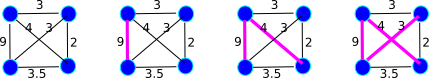
\includegraphics[width=5in]
{chow/spanning-tree.png}
\caption{
Example of finding MST (maximum spanning tree)} 
\label{fig-spanning-tree}
\end{figure}

\begin{figure}[h!]
\centering
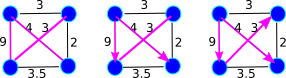
\includegraphics[width=3in]
{chow/tree-dir.png}
\caption{Example of giving directions
to edges of spanning tree.} 
\label{fig-tree-dir}
\end{figure}

Nodes in a Chow-Liu tree can
be rated in
terms
of their relative importance.
Here are 2 possible
metrics
for measuring 
the importance
of a node $\rva$:

\beq
N_{nb}(\rva)=
\text{ number of neighbors of $\rva$}
\eeq

\beq
{\rm traffic}(\rva)=
\sum_{\rvn\in nb(\rva)}
H(\rva:\rvn)
\eeq
For example,
to get a tree with low depth, 
one can choose
as the root node
the node which has 
largest $N_{nb}$, and
if there are several
with the same largest $N_{nb}$,
choose out of those the 
one with the largest traffic.


\section*{Tree Augmented Naive Bayes (TAN)}

Recall from Chapter \ref{ch-naive}
that a Naive
Bayes bnet
consists
of  a class node $\rvc$
with
$n$ children nodes
$\rvx^n$, called the feature nodes. A
Tree Augmented Naive Bayes (TAN) bnet
is a Naive Bayes bnet with 
a 
tree grafted onto it like a chimera.
More precisely,
one starts
with a Naive Bayes bnet 
and adds arrows between
the feature nodes.
The arrows are added in such a way
that the TAN bnet sans node $\rvc$
constitutes a tree.
It's not the most well 
motivated bnet in human
history,
but at least
it adds a bit
of correlation between
the feature nodes
of the Naive Bayes bnet.
Those nodes are independent
at fixed $\rvc$
in the Naive Bayes
bnet, but are no longer so
in the TAN bnet.
See Figs.\ref{fig-naive-tree}
and \ref{fig-tan}
for an example of a TAN bnet.



\begin{figure}[h!]
\centering
$$\xymatrix{
\rvc\ar[d]\ar[dr]\ar[drr]\ar[drrr]\\
\rvx_0&\rvx_1&\rvx_2&\rvx_3
}
\;\;\;\;
\xymatrix{
\rvx_0&\rvx_1
&\rvx_2\ar[l]\ar@/^1pc/[ll]
&\rvx_3\ar[l]
}$$
\caption{bnet for Naive Bayes
with 4 feature nodes
and another bnet for a tree
made of the same feature nodes.}
\label{fig-naive-tree}
\end{figure}

\begin{figure}[h!]
\centering
$$\xymatrix{
\rvc\ar[d]\ar[dr]\ar[drr]\ar[drrr]\\
\rvx_0&\rvx_1
&\rvx_2\ar[l]\ar@/^1pc/[ll]
&\rvx_3\ar[l]
}$$
\caption{
TAN bnet constructed
by merging Naive
Bayes bnet
and tree
bnet
of Fig.\ref{fig-naive-tree}.}
\label{fig-tan}
\end{figure}


The total probability distribution
$P_{TAN}$ for a TAN bnet
can be parameterized as follows.

\beq
P_{TAN}(x^n, c)=P_{TAN}(c)\prod_{i=0}^{n-1}
P_{TAN}(x_i|x_{\mu(i)}, c)
\;.
\eeq

As with Chow Liu trees,
we can attempt
to find a TAN bnet
whose total 
probability $P_{TAN}=P_{\rvt^n, \rvc}$
best approximates
an a priori given probability 
distribution $P=P_{\rvx^n, \rvc}$.

Note that
\begin{claim}

\beq
\argmin_\mu H(\rvx^n, \rvc)
=
\argmax_\mu
\sum_i H(\rvx_i:\rvx_{\mu(i)}| \rvc)
\eeq
\end{claim}
\proof

\beqa
H(\rvx^n, \rvc)
&=&-
\sum_{x^n,c}P(x^n,c)
\left[
\ln P(c)+
\sum_i
\ln P(x_i|x_{\mu(i)}, c)
\right]
\\
&=&-
\sum_{x^n,c}P(x^n,c)
\left[
\ln P(c)+
\sum_i
\ln \left(\frac{P(x_i, x_{\mu(i)}|c)}
{P(x_i|c)P(x_{\mu(x_i)}|c)}
P(x_i| c)
\right)
\right]
\\
&=&
\sum_i H(\rvx_i, \rvc)
-
\sum_i H(\rvx_i:\rvx_{\mu(i)}|\rvc)
\eeqa 
\qed


Following
the same line of
reasoning
that we followed
for Chow-Liu trees,
we conclude that:

If $D_{KL}(P\parallel P_{TAN})$
is minimized over all $P_{TAN}$, then
\begin{enumerate}
\item$P_{TAN}$
inherits
its TPM's 
from $P$, and
\item
$P_{TAN}$ gets
its structure,
which is being parameterized
by 
the function $\mu$,
by
maximizing 
the score defined by

\beq
\text{score}
=\sum_i H(\rvx_i:\rvx_{\mu(i)}|\rvc)
\label{eq-score-tan}
\eeq
\end{enumerate}

One can build a TAN bnet
from empirical data as follows:

Calculate a Chow-Liu Tree
for each $c\in S_\rvc$.
For each of those trees,
create a TAN bnet, and 
calculate its
score given by
  Eq.(\ref{eq-score-tan}).
Keep
the TAN bnet with
the largest score.


\chapter{Counterfactual Reasoning}
\label{ch-counterf}


\section{The 3 Rungs of Causal AI}
According to 
Judea Pearl,
there are 3 rungs in the
ladder of causal AI.
These are (as I see them):
\begin{enumerate}
\item
{\bf Observing Passively:} Collecting 
data
and fitting curves to it,
without any plan 
designed to
investigate Nature's 
causal connections.
\item {\bf Doing causal
experiments:} 
Doing experiments 
consciously designed to
elucidate
Nature's causal connections.
Even cats do this!, but current AI doesn't.
\item {\bf Imagining
 counterfactual situations, Analogizing:}
Imagining gedanken experiments
to further understand
Nature's causal connections,
and to decide what future
courses of action are
more likely to succeed,
even if
those courses of action
are unprecedented, and have never been taken before.
Making
predictions about
 events that have never happened (``counterfactuals")
is a very Bayesian
concern, well out of the purview of 
frequentists. Nevertheless,
humans do such
``analogizing" 
all the time to great advantage.
It becomes
possible if there
is some indirect but similar
data that can be transported
(transplanted, applied)
to the situation of
interest.
\end{enumerate}
Chapter \ref{ch-mpass}
on message passing
is about rung 1.
Chapter \ref{ch-do-calc}
on Do Calculus is about rung 2.
This chapter is dedicated to rung 3.

Judea Pearl 
is fond of discussing rung 3 solely
in terms of SCM.\footnote{SCM are 
what we call DEN. DEN (deterministic systems
with external noise) are discussed in
Chapter \ref{ch-linear-sys}. }
In this chapter,
we define rung 3
without using SCM, using solely
bnets.
This gives a more general
version of rung 3,
because SCM are a subset of bnets.



We will use the
term {\bf intervention operator (or simply ``intervention")} 
to refer to an operator
that maps a bnet to another bnet.
In Chapter \ref{ch-do-calc},
we introduced an intervention operator
 called the {\bf do operator}
$\cald_{\rvx=x}$ (this is our notation for what Pearl 
symbolizes by $do(\rvx)=x$).
The study of counterfactuals 
requires that we
introduce a new
kind of intervention 
operator that we will
call an {\bf imagine operator},
and denote by $\cali_{\rvx\rarrow\rvy}(\tilde{x})$.
These 2 types of interventions 
will be defined 
next.

\section{Do operator}


\begin{figure}[h!]
\centering
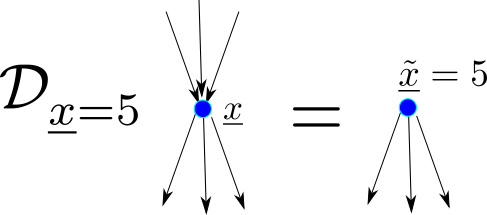
\includegraphics[width=1.75in]
{counterf/rho-op.png}
\caption{Action
of ``do" operator $\cald_{\rvx=5}$
on node $\rvx$.} 
\label{fig-rho-op}
\end{figure}

The do operator $\cald_{\rvx=5}$
is defined graphically in Fig.\ref{fig-rho-op}.
The TPM, printed in blue,
 for node $\tilde{\rvx}$ of Fig.\ref{fig-rho-op},
is given by

\beq\color{blue}
P(\tilde{x})=\delta(5, \tilde{x})
\eeq


The do operator $\cald_{\rvx=5}$
amputates
the incoming arrows of node $\rvx$
and sets the TPM
of the new root node $\tilde{\rvx}$
to a delta function $\delta(
\tilde{x}, 5)$
(or some state of $\rvx$
 other than 5).
Sometimes we call the new node
$\cald\rvx$
instead of 
$\tilde{\rvx}$.

The uses of the do operator are discussed
in detail in Chapter \ref{ch-do-calc}.

\section{Imagine operator}

\begin{figure}[h!]
\centering
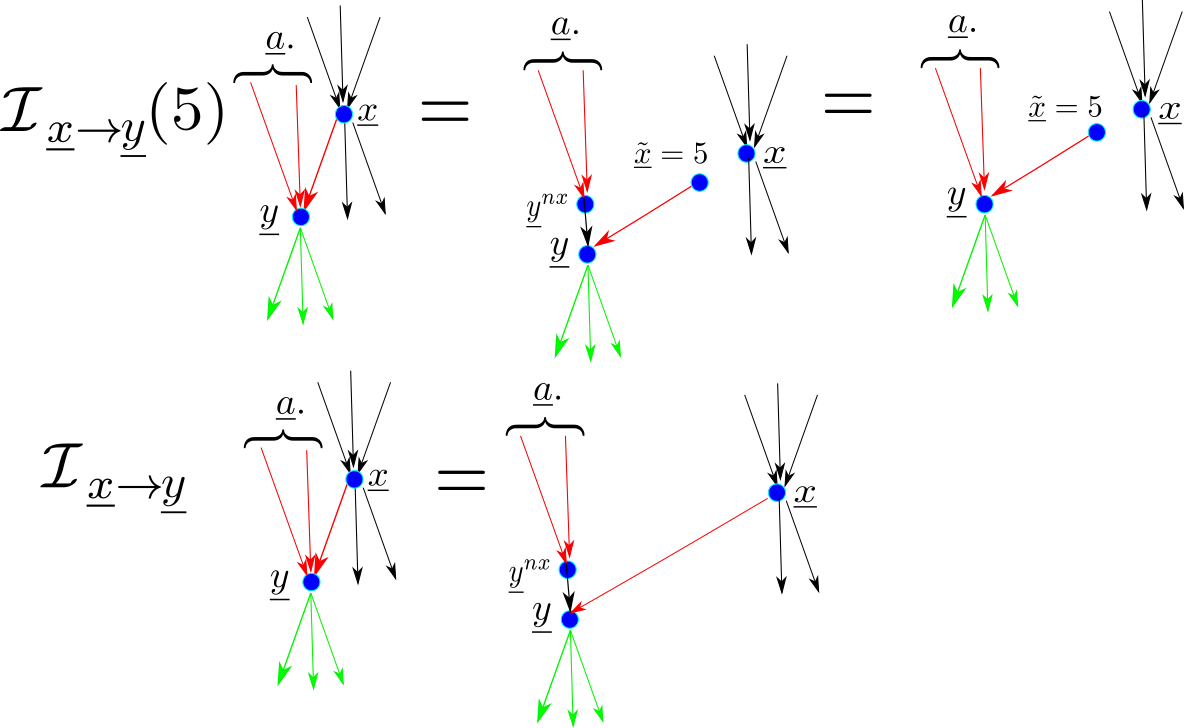
\includegraphics[width=4in]
{counterf/kappa.png}
\caption{Action of ``imagine" operators 
$\cali_{\rvx\rarrow \rvy}(5)$
and $\cali_{\rvx\rarrow \rvy}$
on arrow $\rvx\rarrow \rvy$.
In this figure, $y^{nx}=[y(x)]_{\forall x\in S_\rvx}$,
where $nx=|S_\rvx|$
and $S_\rvx$ is the set of states of node $\rvx$.
} 
\label{fig-kappa}
\end{figure}

The imagine operator  $\cali_{\rvx\rarrow \rvy}(5)$
is defined graphically in Fig.\ref{fig-kappa}.
Note that Fig.\ref{fig-kappa}
actually defines two types 
of imagine operators, the one
with an argument:
$\cali_{\rvx\rarrow \rvy}(5)$,
and the one without an argument: 
$\cali_{\rvx\rarrow \rvy}$.
The TPMs, printed in blue, 
for various nodes in
Fig.\ref{fig-kappa}, are as follows.



\begin{itemize}

\item
For $\cali_{\rvx\rarrow 
\rvy}(\tilde{x})G$

\beq\color{blue}
P(y| \tilde{x}, a.)=
P(y| \rvx=\tilde{x}, a.)
\eeq

\beq\color{blue}
P(\tilde{x})=
\delta(\tilde{x}, 5)
\eeq

\item
For $\cali_{\rvx\rarrow \rvy}G$
\beq\color{blue}
P(y^{nx}| a.)=\prod_{\tilde{x}}
P(\rvy(\tilde{x})=y(\tilde{x})|a.)
\eeq

\beq\color{blue}
P(y|y^{nx}, x)=
\delta(y,y(x))
\eeq
\end{itemize}
The imagine operators 
$\cali_{\rvx\rarrow\rvy}(5)$
and $\cali_{\rvx\rarrow\rvy}$
operate on an arrow
whereas the 
$\cald$ operator
 operates on a node.
$\cali_{\rvx\rarrow\rvy}(5)$
deletes
arrow $\rvx\rarrow\rvy$
and
creates a new root node 
$\tilde{\rvx}$
and a new arrow
$\tilde{\rvx}\rarrow \rvy$.
Sometimes we call
the new node
$\cali_\rvy\rvx$
instead of
 $\tilde{\rvx}$. 
$\cali_{\rvx\rarrow\rvy}$
creates 
a new node $\rvy^{nx}$
and an arrow $\rvy^{nx}\rarrow \rvy$.



\begin{figure}[h!]
$$
\begin{array}{ccccc}
\xymatrix{
&\rvx\ar@[red][ddr]\ar[ddl]
\\
&&&
\\
\rvd\ar@[red][rr]
&
&\rvy\ar@[green][r]
\ar@[green][ur]
&
}
&
\xymatrix{
&&\rvx\ar[ddll]\ar@[red][d]
\\
&&[\rvy(0),\rvy(1)]\ar[d]
&
\\
\rvd\ar@[red][rr]
&
&\rvy\ar@[green][r]
\ar@[green][ur]
&
}
\\
\\
G&G_+=\cali_{\rvd\rarrow\rvy}G
\end{array}
$$
\caption{How 
 imagine operator 
arises in 
Potential Outcomes (PO)
theory.
} 
\label{fig-counterf-G-im-y0-y1}
\end{figure}
Fig.\ref{fig-counterf-G-im-y0-y1}
shows how the
imagine operator arises
in Potential Outcomes (PO) theory.
PO theory is discussed extensively
in Chapter \ref{ch-pot-out}.
As you can see, PO theory
only uses a limited version
of the 3 rungs
of causal inference, because it 
doesn't use the do-operator,
and it only uses one 
of 2 possible types of
imagine operators.
Furthermore,
it assumes a
very limited triangular DAG.


\begin{figure}[h!]
\centering
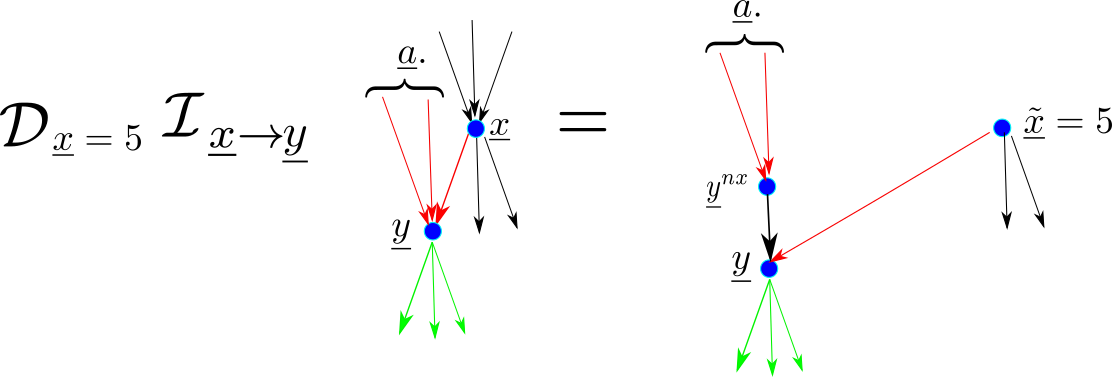
\includegraphics[width=3.5in]
{counterf/rho-kappa.png}
\caption{$\cald_{\rvx=5}\cali_{\rvx\rarrow \rvy}G$
gives a connection
between do and imagine operators.
} 
\label{fig-rho-kappa}
\end{figure}

Fig.\ref{fig-rho-kappa}
gives  a connection
between do and imagine
operators.
We see
from that figure that
for $\cald_{\rvx=\tilde{x}}
\cali_{\rvx\rarrow\rvy}G$, we have\footnote{In the
notation favored by Pearl, Eq.(\ref{eq-connect-do-imag})
 would be
$$P(y|do(X)=\tilde{x}, a.)=P(Y_{\tilde{x}}=y|a.)$$}
\beq
P(y|\cald\rvx=\tilde{x}, a.)=P(\rvy(\tilde{x})=y|a.)
\label{eq-connect-do-imag}
\eeq


One can define
a {\bf do-imagine-calculus}
whose
objective
is to 
express
probabilities such as 
$P(\rvy|\cald\rvr=r,
\cali_\rvb \rvs=s, t)$
in terms of observable 
probabilities
that do not
contain
any do or imagine
operators in them.
As with
Do Calculus,
this reduction
is not 
always possible,
and we say a probability is
{\bf $\cald$-identifiable},
{\bf $\cali$-identifiable}
or
{\bf $\cald\cali$-identifiable}
if it  can be 
expressed without do, imagine
or both operators.


\chapter{Decision Trees}\label{ch-dtree}
This chapter is based 
mainly on Ref.\cite{stu-nor-book}.

\begin{figure}[h!]
\centering
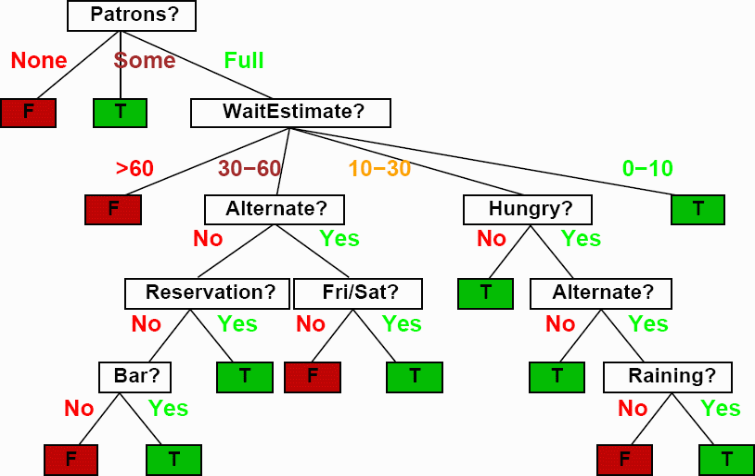
\includegraphics[width=4in]
{dtree/dtree-waiting.png}
\caption{Example of dtree taken from Ref.\cite{stu-nor-book}} 
\label{fig-dtree-waiting}
\end{figure}


\begin{figure}[h!]
\centering
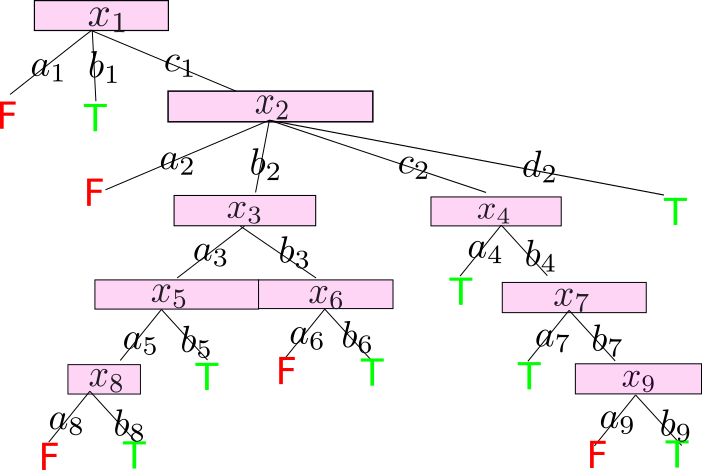
\includegraphics[width=3.2in]
{dtree/dtree-waiting-labels.png}
\caption{Fig.\ref{fig-dtree-waiting} with
abridged labels.} 
\label{fig-dtree-waiting-labels}
\end{figure}

\begin{figure}[h!]
\centering
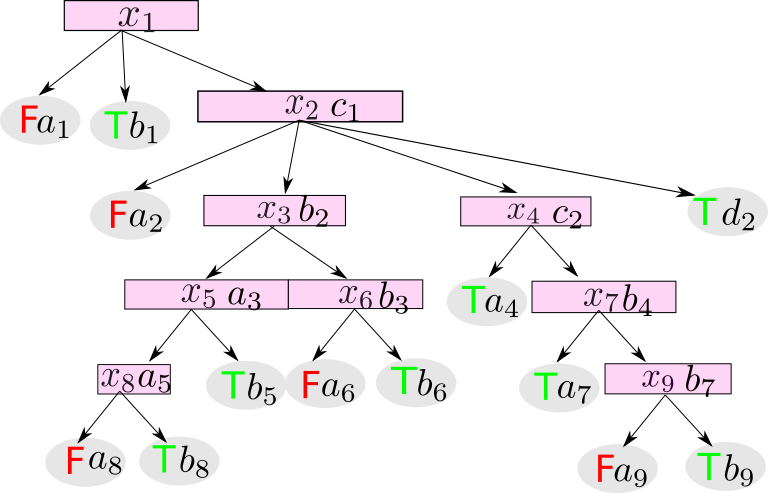
\includegraphics[width=3.2in]
{dtree/dtree-waiting-dags.png}
\caption{Fig.\ref{fig-dtree-waiting-labels}
converted to a bnet.} 
\label{fig-dtree-waiting-dags}
\end{figure}

Fig.\ref{fig-dtree-waiting}
shows a typical decision tree (dtree).
This example was taken
from Ref.\cite{stu-nor-book},
where it is analyzed
in detail.
As you can see,
a dtree contains two main types
of nodes: the non-leaf nodes,
and the leaf nodes.
The {\bf non-leaf nodes} pose
{\bf questions}. In general,
the {\bf answers}\footnote
{The {\bf question-answer pairs}
in dtrees are
also called
{\bf attribute-value pairs}.
Attributes are also
called {\bf features}.}
 to those
questions can
be multiple choices with
two or more choices.
For each of those choices,
a tree branch labeled by the choice
 comes down from the 
question node.
The {\bf leaf nodes} represent
endpoints, goals, final
conclusions, etc.
Dtrees can be viewed
as classifiers. They
take in a large amount 
of information about a population 
and compress that information
to just a few classes.
If $S_\rvc$ is the 
set of distinct leaf node labels,
then we call each
$c\in S_\rvc$
a  {\bf class of the classifier}.
In the case of
Fig.\ref{fig-dtree-waiting},
$S_\rvc=\{False, True\}$.

Dtrees can be used 
with
probabilities attached to each node, or without
probabilities
(as a
plain undirected graph(UG)).
This is analogous to bnets,
which can be used with
probabilities attached to each node
 (as DAGs with
TPMs specified for each node) or without
probabilities (as plain
DAGs).
Dtrees differ 
from bnets in that
their tree branches 
are labelled, whereas bnet arrows
 aren't labelled.
Also,
whereas the nodes of
a bnet carry a matrix of 
probabilities (the TPM),
the nodes of a dtree carry
just a column vector
of probabilities
which represents
a single 
probability distribution.
Henceforth,
we will refer to
the column vector
of probabilities
carried by each node of a dtree
as its {\bf Transition
Probability Vector (TPV)}.
Without the TPVs,
a dtree can be used 
as a deterministic classifier,
to classify inputs.
With the TPVs,
it can be used as a 
probabilistic sampler (to generate
random samples.)

\section{Transforming a dtree into a bnet}
A trivial 
observation
that is seldom made
in the dtree pedagogical literature
is that every dtree 
maps into a special bnet, 
let's call it
its ``image" bnet,
in a very natural way.
We use the dtree
of Fig.\ref{fig-dtree-waiting}
as an example to show 
how to do this. As 
a first 
step,
we go from
Fig.\ref{fig-dtree-waiting}
to
Fig.\ref{fig-dtree-waiting-labels}
by
replacing
all the labels of the
nodes and of the branches of
the dtree 
by abridged symbols. 
Next, we go 
from Fig.\ref{fig-dtree-waiting-labels}
to Fig.\ref{fig-dtree-waiting-dags},
by replacing all tree branches 
by arrows pointing down,
 and by
moving the tree branch labels 
down so that they
become a suffix to the question 
that the tree branch leads to.
At this point,
we have created
Fig.\ref{fig-dtree-waiting-dags},
which constitutes
the DAG of the image bnet.
It remains for us to define
a TPM for each node
of this DAG.

\begin{table}[]
\centering
\begin{tabular}{|l|l|l|l|}
\hline
$P(x|a)$ & \cellcolor[HTML]{ECF4FF}$a=a_0$ & \cellcolor[HTML]{ECF4FF}$a\in S^-_\rva-\{a_0\}$ & \cellcolor[HTML]{ECF4FF}$null$ \\ \hline
\cellcolor[HTML]{ECF4FF}0 & $p_0$ & 0 & 0 \\ \hline
\cellcolor[HTML]{ECF4FF}1 & $p_1$ & 0 & 0 \\ \hline
\cellcolor[HTML]{ECF4FF}$\vdots$ & $\vdots$ & 0 & 0 \\ \hline
\cellcolor[HTML]{ECF4FF}$N^-_\rvx-1$ & $p_{N_\rvx-1}$ & 0 & 0 \\ \hline
\cellcolor[HTML]{ECF4FF}$null$ & 0 & 1 & 1 \\ \hline
\end{tabular}
\caption{TPM of a node of a dtree image bnet.}
\label{tab-dtree-tpm}
\end{table}


Table \ref{tab-dtree-tpm}
gives the 
TPM $P(x|a)$
for a node $\rvx$
with single parent $\rva$
of a dtree image bnet. 
Say node $\rvx$ has 
a set $S^-_\rvx$
of possible tree branches
coming out of it. 
Let $N^-_\rvx = |S^-_\rvx|$.
Let $S_\rvx=S^-_\rvx\cup \{null\}$
and $N_\rvx=|S_\rvx|=N^-_\rvx+1$.
Define $S^-_\rva$, $N^-_\rva$,
$S_\rva$
and $N_\rva$
analogously for node $\rva$.
In Table \ref{tab-dtree-tpm},
$S^-_\rvx=\{0,1, \ldots, N^-_\rvx-1\}$
and 
$a_0$ is the value
of node $\rva$ which 
labels the tree branch
connecting nodes $\rva$ and $\rvx$.
$\vec{p}=(p_0, p_1, \ldots, p_{N_\rvx-1})$
is a probability
distribution 
associated with node $\rvx$,
its TPV.
TPVs
can be learned from
a dataset
following
the dtree Structure Learning (SL)
algorithm
discussed in Section \ref{sec-dtree-sl}.

Table \ref{tab-dtree-tpm}
also applies when node $\rvx$
is a leaf node,
except that for leaf nodes,
$\vec{p}$ is one hot (i.e., 
all components are zero 
except for one 
component which is 1).
Also, all 
leaf nodes
$\rvx$ have the same $S^-_\rvx$,
namely $S_\rvc$.


Adding a null state
to the set of states (SOS) of each node 
of the image bnet
is necessary
because, once $null$
is added 
to the SOS of any node,
it must be added to the SOS
 of all descendant
nodes.
$null$ must be added to the 
SOS of the children of
the root node
to
take care of the situations
when those first children
don't receive the state 
they were expecting from their
parent, i.e., the root node.


When drawing dtrees,
some people put
info 
like explanations 
and probabilities on the
branches
of  the dtree.
That
info can all
be preserved
in the TPM
and  the
node names and
 node state names
of the image bnet nodes.
One can also place info
inside tool tips attached to
the node name and node state names.
Often,
the pedagogical literature
states that 
dtrees are more explicit and  
carry
more info than their
image bnets,
but if one 
follows the above
prescriptions,
both can carry
the same info.



A naive Bayes (NB) bnet 
(see Chapter \ref{ch-naive})
consists of a single ``class node"
with states $S_\rvc$ that fans
out with arrows 
pointing to the
``feature nodes".
If each leaf node
of a NB bnet
fans out into 
a set of new leaf
nodes, and those new
leaf nodes
also
fan out
and so on,
we get a 
generalized NB bnet.
Let's call
this type of tree bnet an $NB^*$ bnet.
An $NB^*$ bnet
has the same graph structure
as the image bnet of a dtree,
but it's more general,
because its 
TPMs are more general. 
Each 
TPM of a $NB^*$ bnet
 can have several non-trivial
columns instead of just one
TPV= $\vec{p}$.


\section{Structure Learning for  Dtrees}\label{sec-dtree-sl}



Let

$J_0=\{0,1, \ldots, nj-1\}$

$\Sigma=\{0,1,2, \ldots,nsam-1\}$

$DS=\{(\s, x^\s, c^\s): \s\in \Sigma\}$ be a dataset

$\s\in \Sigma$ be an individual (a sample)
from a population, 

$x^\s\in S_\rvx$ be the {\bf
feature (attributes, questions) vector}.
$S_\rvx= S_{\rvx_0}\times S_{\rvx_1}
\times\ldots\times S_{\rvx_{nj-1}}$,
$x=(x_0, x_1, \ldots, x_{nj-1})\in S_\rvx$, 
$x_j\in S_{\rvx_j}$


$c^\s\in S_\rvc$ be a {\bf classification class}

We will
assume $S_\rvx$ and $S_\rvc$ are finite sets.

Building a {\bf classifier $Y$} 
(curve fit) for a dtree means
finding a deterministic
function $Y:S_\rvx\rarrow S_\rvc$ 
such that 
$c^\s \approx Y(x^\s)$
for all $\s\in \Sigma$.
If we divide
the population
$\Sigma$ 
into two large 
disjoint
sets, a {\bf training set} $\Sigma_{train}$
and a {\bf validation set} $\Sigma_{vali}$,
and if $c^\s \approx Y(x^\s)$ very closely
for $\s\in \Sigma_{train}$
but fits poorly
for $\s\in \Sigma_{vali}$,
then we say the classifier  $Y$
suffers from {\bf overfitting}.
We can learn the structure
and TPVs of a dtree from a dataset $DS$,
by using the
dtree {\bf Structure Learning (SL)}
algorithm that we will 
discuss in detail later. However,
that algorithm
is prone to produce
a classifier $Y$ that overfits.
Two techniques 
commonly used to 
reduce the effects of overfitting
are {\bf pruning}  and 
{\bf Random Forest (RF)}
(see Chapter \ref{ch-rforest}).
Pruning just means somehow
removing nodes that are
too specific. 
An RF is an ensemble of dtrees 
that one averages over.
In this chapter, we will only deal
with a single dtree,
not an ensemble of them. 

Dtree SL was invented in 1984-1986 so it
is fairly old.
Many in the AI
community 
consider dtrees old fashioned
compared to neural nets.
But dtrees 
are {\bf interpretable} whereas neural nets aren't.\footnote{
To be precise, only
plain dtrees without boosting or
 bagging
are interpretable.
Dtrees used within boosting
(see Chapter \ref{ch-adaboost} on AdaBoost
and
Chapter \ref{ch-xgboost} on XGBoost)
or bagging
(see Chapter \ref{ch-rforest} on Random Forest)
gain much
accuracy but lose
{\bf interpretability}.}
Bnets are interpretable too.


Below,
we give the standard
algorithm for SL
of a dtree, in the form
of pseudo-code.
But first,
we define
two quantities,
Information Gain and
Gini,
that are 
used in that 
pseudo-code.


\subsection{Information Gain, Gini}
This section uses various Shannon Information Theory
entropies. Our 
notation for those
entropies
is described in Chapter \nameref{ch-conventions}.


Call a {\bf separation ability measure} (SAM)
a measure used 
to decide, when 
constructing a dtree from a dataset,
in what order 
to ask the questions
about the feature vector $x$.
The question order is decided
by searching 
over all so far unused questions
for the question with 
the largest SAM.\footnote{SAM
is also called, somewhat
confusingly, the splitting
criterion and Gain.}



\begin{figure}[h!]
$$
\xymatrix{
&
\\
\rvx_j\ar[r]_{\rvx_j=x_j}
\ar[ru]^{\rvx_j=x_j'}&
\\
\{N_j(c,x_j)\}_{c\in S_\rvc, x_j\in S_{\rvx_j}}
\\
\sum_{c\in S_\rvc}N_j(c,x_j)=N_j(x_j)
\\
\sum_{x_j\in S_{\rvx_j}}N_j(c,x_j)=N_j(c)
&
\sum_{c\in S_\rvc}N_j(c)=
\sum_{x_j\in S_{\rvx_j}}N_j(x_j)=N_j
}
$$
\caption{
Some population numbers associated
with the nodes of a dtree. $N_j(c, x_j)$ is the number
of individuals $\s$
in the population that reaches node $j$,
belonging to class $c$ and having $\rvx_j=x_j$.} 
\label{fig-dtree-notation}
\end{figure}
\begin{figure}[h!]
$$
\xymatrix{
\rvj
\ar[r]\ar@/^1pc/[rr]
&
\rvx_j \ar[r]
&
\rvc
}$$
\caption{Bnet derived from population
numbers in Fig.\ref{fig-dtree-notation}}
\label{fig-class-bnet}
\end{figure}



Fig.\ref{fig-dtree-notation}
defines some population numbers
associated
with the nodes of a dtree.
From these population numbers, we can define
the bnet in Fig.\ref{fig-class-bnet}.
The TPMs, printed in blue,
for the (non-root) nodes of this bnet, are as follows

\beq\color{blue}
P(c|x_j,j)=
\frac{N_j(c,x_j)}
{N_j(x_j)}
\eeq

\beq\color{blue}
P(x_j|j)=
\frac{N_j(x_j)}
{N_j}
\eeq
where $j\in J_0$
$x_j\in S_{\rvx_j}$, and
$c\in S_\rvc$ is a class node.



One can define the following 
information theory quantities\footnote{
The average of $H(\rvc:b)$ over
$b$ is $H(\rvc:\rvb)=\sum_bP(b)
H(\rvc:b)$.
Likewise,
the average of
$H(\rvc|b)$ over $b$ is 
$H(\rvc|\rvb)=\sum_b P(b)H(\rvc|b)$.
$H(\rvc:\rvb)$ 
becomes $H(\rvc:b)$
and $H(\rvc|\rvb)$
becomes $H(\rvc|b)$
when there is no $b-$prior (i.e., 
$P(b)$ is a delta function).
}
associated with the bnet Fig.\ref{fig-class-bnet}.


\beqa
INFO\_fin_j&=& 
-\sum_c P(c|j)\ln P(c|j)
\\
&=&
H(\rvc|j)
\\
\eeqa




\begin{align}
INFO\_init_j
&=
\sum_{x_j\in S_{\rvx_j}} P(x_j|j)H(\rvc|x_j,j)
\\
&=
H(\rvc|\rvx_j , j)
\end{align}



\beqa
IG_j&=&
INFO\_fin_j- INFO\_init_j
\\
&=&
H(\rvc|j)-H(\rvc|\rvx_j , j)
\\
&=& H(\rvc:\rvx_j |j)
\label{eq-info-gain}
\eeqa
$IG_j$
is called the {\bf
information gain
for node $\rvx_j$}.
Maximizing this mutual information
produces 
a node $\rvx_j$ that has 
a large correlation
to a class $c$.
If the  
goal is to reach
a point 
where each leaf node is
closely correlated
to a different class,
then maximizing the
Information Gain
of each new node
is a greedy move
towards that goal.
Thus, Information Gain
is a good 
SAM
for dtree SL.

Note that if we approximate

\beqa
\ln  P(c|x_j)
&\approx&
\ln [1 + P(c|x_j)-1]
\\
&\approx&
P(c|x_j)-1
\eeqa
in $H(\rvc|x_j)$,
we get what is called 
the {\bf Gini (or Gini Index)
for node $\rvx_k$}:


\beqa
H(\rvc|x_j)
&=&
-\sum_c P(c|x_j)\ln P(c|x_j)
\\
&\approx&
1 -\sum_{c\in S_{\rvc}} P(c|x_j)^2
\eqdef
 Gini_{x_j}
\eeqa
$Gini_{x_j}$
is a fairly good
polynomial approximation
to $H(\rvc|x_j)$.
It is computationally
much less expensive than
$H(\rvc|x_j)$,
because it does not
require computing a log.

We say 
a probability 
distribution $P_\rvx$, is {\bf pure (i.e., deterministic)}
 if $P_\rvx(x)=\delta(x, x_0)$. $Gini_{x_j}$
 and $H(\rvc|x_j)$ are both always
non-negative.
They both vanish iff  
$P(c|x_j)$ is pure.
Thus, $Gini_{x_j}$ and  $H(\rvc|x_j)$ 
are both good measures of  {\bf class impurity}.

The {\bf average Gini of node $\rvx_j$} is defined as

\beq
AGini_j
=
\sum_{x_j\in S_{\rvx_j}}
P(x_j|j)
 Gini_{x_j}
\;.
\eeq
It measure 
the average impurity
of the children of node $\rvx_j$.



\begin{mdframed}[hidealllines=true,backgroundcolor=gray!10]
In practice, the
SL algorithm
is done recursively.
Each 
recursion
step 
decides
which feature $x_j$
will be the root 
node of the current tree.
For all ``candidate" features
(i.e., all $\rvx_j$
that haven't been used yet 
as tree nodes), one
calculates
$IG_j$,
either
exactly
or approximately via Gini's,
using the following formula:

\beq
IG_j=
\underbrace{H(\rvc|j)}_{\approx Gini_j}
-
\sum_{x_j\in S_{\rvx_j}}
P(x_j|j)
\underbrace{H(\rvc|x_j)}_
{\approx Gini_{x_j}}
\eeq
One then chooses $j=\argmax_j IG_j$. This
maximizes the $\rvc-\rvx_j $ correlation.

Alternatively,
some software programs use
the average Gini
$AGini_j$
as their SAM. They
choose
as root node
 $j=\argmin_j AGini_j$.
This minimizes the average impurity
of the children of node $j$.
Since $IG_j$
differs from $AGini_j$ by $H(\rvc|j)$,
maximizing $IG_j$
and
minimizing $AGini_j$
might lead  to different results.
\end{mdframed}
\hrule\noindent{\bf Example of calculation of $AGini_j$ 
and $IG_j$}

Suppose we deduce from a dataset
the numbers in the yellow cells
in Table \ref{tab-temp-gini}.
These numbers are repeated in  Fig.\ref{fig-stump-3cildren}.
Then we can calculate the white cells as follows: 

% Please add the following required packages to your document preamble:
% \usepackage[table,xcdraw]{xcolor}
% If you use beamer only pass "xcolor=table" option, i.e. \documentclass[xcolor=table]{beamer}
\begin{table}[h!]
\centering
\begin{tabular}{|l|l|l|l|}
\hline
$j=temp?$ & \cellcolor[HTML]{CBCEFB}$x_j=hot$ & \cellcolor[HTML]{CBCEFB}$x_j=med$ & \cellcolor[HTML]{CBCEFB}$x_j=cold$ \\ \hline
\rowcolor[HTML]{FFFFC7} 
\cellcolor[HTML]{9AFF99}$c=play$ & 3 & 3 & 3 \\ \hline
\rowcolor[HTML]{FFFFC7} 
\cellcolor[HTML]{FFCCC9}$c=stay$ & 1 & 2 & 2 \\ \hline
$Gini$ & 0.375 & 0.48 & 0.48 \\ \hline
\multicolumn{4}{|l|}{$AGini=0.45$} \\ \hline
$H(\rvc|x_j)$ & $\approx 0.375$ & $\approx 0.48$ & $\approx 0.48$ \\ \hline
\multicolumn{4}{|l|}{$IG\approx 0$} \\ \hline
\end{tabular}
\caption{Evaluating AGini and IG for node $temp$.}
\label{tab-temp-gini}
\end{table}



\begin{figure}[h!]
\centering
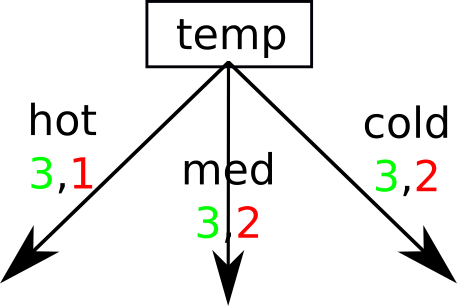
\includegraphics[width=1.5in]
{dtree/stump-3children.png}
\caption{Tree stump
corresponding to Table \ref{tab-temp-gini}.}
\label{fig-stump-3cildren}
\end{figure}



\begin{itemize}
\item Gini(hot)$=1-(3/4)-(1/4)=0.375$
\item Gini(med)$=1-(3/5)^2-(2/5)^2=0.48$
\item Gini(cold)$=1-(3/5)^2-(2/5)^2=0.48$
\item AGini $ = (4/14)(0.375)+
(5/14)(0.48) + (5/14)(0.48) = 0.45 $
\item IG $\approx [1 -(6/9)^2-(3/9)^2]-AGini= 
0.44-0.45\approx 0$
\end{itemize}

This gives
the AGini and IG for just one 
candidate root node.
We would have
to calculate
AGini (or IG) for all
possible candidates
and choose the candidate
with the lowest AGini (or highest IG).


\section{Information Gain Ratio}

The Information Gain Ratio (IGR) is an alternative SAM.

\beqa
IGR_j
&=&
\frac{IG_j}{H(\rvx_j |j)}
\\
&=&
\frac{H(\rvc:\rvx_j |j)}{H(\rvx_j |j)}
\\
&=&
\frac{H(\rvx_j |j)-H(\rvx_j |\rvc, j)}
{H(\rvx_j |j)}
\\
&=&
1 - \frac{H(\rvx_j |\rvc, j)}{H(\rvx_j |j)}
\eeqa

$0\leq IGR_j\leq 1$

$IGR_j=0$ iff $H(\rvx_j |\rvc, j)=H(\rvx_j |j)$.




\subsection{Pseudo-code}

Below,
we give the standard
algorithm for SL
of a dtree, in the form
of pseudo-code.
The strategy
employed by
the algo
is to assume an incoming
population into the current root node,
then
determine the feature $x_j$
 that best separates that 
incoming
population. The feature
$x_j$ is chosen so as to maximize
$IG_j$
(or minimize $AGini_j$). This
process is repeated by nominating
the end of each new branch to be
the current root node.
Features can appear as a node 
more than once, so the order in 
which nodes are split does not matter.
In essence, what we are doing is
performing a top-down, greedy search
through the space of possible dtrees.

The pseudo-code below describes the following 
historically important
software programs:
\begin{itemize}
\item CART (Classification and Regression Trees),
invented by Breiman et al in 1984. Uses $AGini_j$ as SAM.
\item
ID3 (Iterative Dichotomiser 3)
invented by Quinlan in 1986. Uses $IG_j$ as SAM.
C4.5/C5.0 are successors to ID3.
\end{itemize}

Thus, CART and ID were 
invented independently around the same time.
The main difference between them is the SAM
being used.


The pseudo-code below
uses the majority function
defined in Chapter \nameref{ch-conventions}.


\begin{algorithm}
	\DontPrintSemicolon
    \SetKwInOut{KwIn}{Input}
    \SetKwInOut{KwOut}{Output}
    \caption{Pseudo-code for learning a dtree from a dataset}
	\KwIn{dataset $DS=\{(\s, x^\s, c^\s): \s\in \Sigma\}$,\\ 
	set of currently available node indices 
	$J$, where $J\subset J_0$}
	\KwOut{tree $T$,\\
		population numbers $\{(r,c,x_r,N_r(c, x_r)):
			r\in J_0, c\in S_\rvc,
			x_r\in S_{\rvx_r}\}$ stored globally}
	\;
	From $DS$, calculate $J_0$, $S_\rvc$, $S_{\rvx_i}$ for each $i$ \\
	$c^\s$ is called the target feature/attribute.\\
	$J\larrow J_0$\;
	\SetKwFunction{FMain}{learn\_dtree}
	\SetKwProg{Fn}{Function}{:}{}
	\Fn{\FMain{$DS, J$}}{
		$\Sigma\larrow$ set of all $\s$ in $DS$\; 
		\If{$\{c^\s:\s\in\Sigma\}=\{c\}$ }{
			$T\larrow$ one node tree with leaf node label= $c$\;
		}
		\ElseIf{$J=\emptyset$}{
			$T\larrow$ one node tree with leaf node label=
			{\tt majority}$([ c^\s:\s\in\Sigma])$\;
		}
		\Else{
			$r\larrow \argmax_{j\in J}IG_j(DS)$
			\tcp{or replace $\argmax_{j\in J}IG_j$ 
			by $\argmin_{j\in J}AGini_j$}\;
			from $DS$, calculate $\{(r,c,x_r, N_r(c,x_r)):
			c\in S_\rvc,x_r\in S_{\rvx_r} \}$ and 
			store it globally\;
		\For{$v\in S_{\rvx_r}$}{
			\tcc{Notice that $J$ is the same every time repeat this loop,
			so order in which $v\in S_{\rvx_r}$ are called does not matter.
			Furthermore, this means that multiple tree nodes may be labeled by same feature.}
			On current tree $T$, add  a branch below $\rvx_r$ with label 
			``$\rvx_r = v$"\;
			$DS|_{\rvx_r=v}\larrow$ subset of $DS$ with $\rvx_r = v$\;
			\If{$DS|_{\rvx_r=v}=\emptyset$}{
				below the new branch add a \\leaf node labeled = 
				{\tt majority}$([c^\s:\s\in\Sigma])$\;
			}
			\Else{
				below the new branch add \\
				subtree =$ {\tt learn\_dtree}
				(DS|_{\rvx_r=v}, J-\{r\})$\;
			}			
    	}
		}
		\KwRet $T$\;
	}
\end{algorithm}


\chapter{Digital Circuits}

\begin{figure}[h!]
\centering
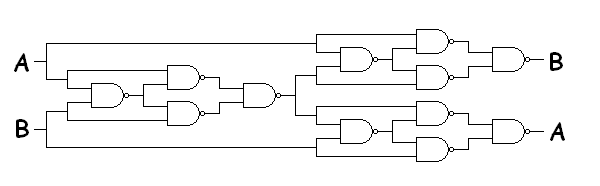
\includegraphics[width=6in]{d-ckt/d-ckt.png}
\caption{Typical digital circuit
of NAND gates.}
\label{fig-d-ckt}
\end{figure}

{\bf Digital (logic) gate:} node with
$na$ input ports and $nx$ output ports
which represents a function

\beq
f:\bool^{na}\rarrow \bool^{nx}
\;.
\label{eq-f-gate}
\eeq

Suppose

$a^{na}=(a_i)_{i=0, 1,\dots, na-1}$ 
where $a_i\in \bool$,

$x^{nx}=(x_i)_{i=0, 1,\dots, nx-1}$ 
where $x_i\in \bool$. 

$f$ maps $a^{na}$ into $x^{nx}$.

{\bf Digital circuit (dcircuit)} = circuit of digital gates.

\begin{figure}[h!]
\centering
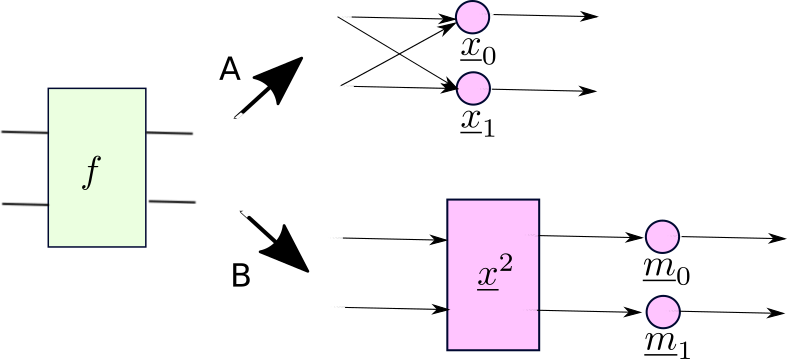
\includegraphics[width=3in]{d-ckt/d-ckt-2ops.png}
\caption{2 options
for mapping dcircuit node with
multiple output ports into bnet.}
\label{fig-d-ckt-2ops}
\end{figure}

\section{Mapping any
dcircuit to a bnet} 
\subsection{Option A of Fig.\ref{fig-d-ckt-2ops}}
\begin{enumerate}
\item
Replace every dcircuit  gate 
described by Eq.(\ref{eq-f-gate})
by
$nx$ bnet nodes $\rvx_i$
for $i=0, 1, \ldots, nx-1$
such that

\beq\color{blue}
P(x_i|a^{na})=\delta(x_i, f_i(a^{na}))
\eeq
\item
Replace
all connectors of the dcircuit
by arrows 
pointing in the direction
of the bit flow.

\end{enumerate}

\subsection{Option B of Fig.\ref{fig-d-ckt-2ops}}
\begin{enumerate}
\item
Replace every dcircuit  gate 
described by Eq.(\ref{eq-f-gate})
with
one bnet node called $\rvx^{nx}$
and, if $nx>0$, 
$nx$ ``marginalizer nodes" $\rvm_i$
for $i=0, 1, \ldots, nx-1$, such that

\beq\color{blue}
P(x^{nx}|a^{na})=
\delta(x^{nx}, f(a^{na}))
\;,
\eeq
and
\beq\color{blue}
P(m_i|x^{nx})=
\delta(m_i, x_i)
\;.
\eeq


\item
Replace
all connectors of the dcircuit
by arrows 
pointing in the direction
of the bit flow.



\end{enumerate}
\hrule 
Options A and B don't work
for digital circuits 
with feedback loops 
such as flip-flops.
Those could probably
be modeled with 
dynamical bnets.
\chapter{Do-Calculus}\label{chap-do-calc}


The do-calculus and associated ideas were
invented by
Judea Pearl and collaborators.
This chapter is 
based on Judea Pearl's
books. (See \ref{ch-nav-pearl}).


When
doing
do-calculus,
it is 
convenient
to separate
the nodes
of a bnet
into
2  types:
{\bf visible (observed)},
and {\bf non-visible (not observed,
hidden)},
depending
on
whether data
describing
the
state 
of that
node
is available 
(visible) or not (non-visible).
In this chapter, hidden nodes will 
be indicated 
in a bnet
diagram by
either: (1)
enclosing
their random variable
in a box (as
if it were inside a black box) or
(2) making
the arrows
coming
out of them
dashed.
Accordingly, 
the 
3 diagrams 
in
Fig.\ref{fig-hidden-dashes}
all mean the same thing.

A {\bf confounder node
for $\rvx$ and $\rvy$}
(such as node
$\rvc$
in Fig.\ref{fig-hidden-dashes})
is a hidden node 
with arrows
pointing
from it to
both
$\rvx$ and $\rvy$.
In other words, it's
an unobserved common
cause of $\rvx$ and $\rvy$.

In this book,
we will refer
to a path
all of whose nodes are
observed as an {\bf opath}.



\begin{figure}[h!]
$$\xymatrix{
&*+[F]{\rvc}\ar[dl]\ar[dr]
\\
\rvx\ar[rr]&&\rvy
}
\;\;\;
\xymatrix{
\rvx\ar@{-->}@{<-->}@/^2pc/[rr]
\ar[rr]&&\rvy
}
\;\;\;
\xymatrix{
&\rvc\ar@{-->}[dl]\ar@{-->}[dr]
\\
\rvx\ar[rr]&&\rvy
}$$
\caption{
These 3 diagrams
are equivalent.
They
mean that node $\rvc$
is hidden.
Node $\rvc$
is implicit
in the
middle diagram.}
\label{fig-hidden-dashes}
\end{figure}



Define
an
operator
$\rho_\rvx$
that acts on
a node
$\rvx$
of a bnet
to
delete
all
the 
arrows
entering
$\rvx$,
thus
coverting
$\rvx$
into
a new
node $\rho \rvx$
that
is a root node.
Define 
an analogous 
operator
$\lam\rvx$
that acts on
a node
$\rvx$
of a bnet
to
delete
all
the 
arrows
leaving
$\rvx$,
thus
converting
$\rvx$
into
a new
node $\lam \rvx$
that
is a leaf node.
$\rho_\rvx$
and
$\lam_\rvx$
are
depicted
in Fig.\ref{fig-do-rho-lam}.



\begin{figure}[h!]
\centering
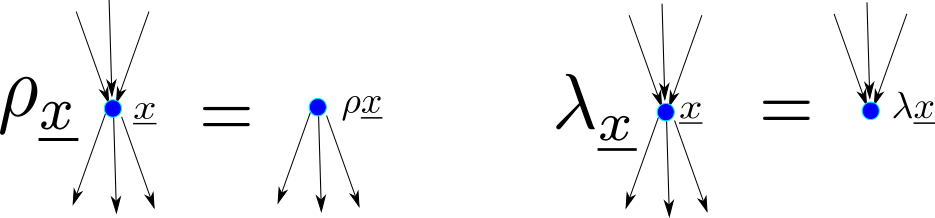
\includegraphics[width=4in]
{do/do-rho-lam.png}
\caption{
The operator $\rho_\rvx$
converts node $\rvx$
into a root node $\rho \rvx$.
The operator $\lam_\rvx$
converts node $\rvx$
into a leaf node $\lam\rvx$.
} 
\label{fig-do-rho-lam}
\end{figure}


If
you don't
know yet
what we mean by a
a multi-node
$\rva.$, see
Chapter \ref{ch-bnet-def}

Given a bnet
$G$,
we define
as follows
the operators
$\rho_{\rva.}$
and
$\lam_{\rva.}$
for a multi-node
$\rva.$.

\beq
\rho_{\rva.}G =
\left[\prod_j \rho_{\rva_j}\right]G
\;,\;\;\;\;
\lam_{\rva.}G =
\left[\prod_j \lam_{\rva_j}\right]G
\;.
\eeq

Consider a bnet 
whose totality of nodes
is labeled $\rvX.$.
Recall that 

\beq
P(X.)=
\prod_j P(X_j|(X_k)
_{k:\rvX_k\in pa(\rvX_j)})
\;.
\eeq

Define an
operator $\rho$
that acts as follows\footnote{As usual,
$\caln(!x)$ denotes 
a constant 
that is independent of $x$.}: Let
$X.-a.=(X_k)_{k:\rvX_k\notin \rva.}$.

\beqa
P(X.-a.|\rho\rva.=a.)
&=&
\caln(!(X.-a.))
\frac{P(X.)}
{
\prod_{j:\rvX_j\in \rva.}
P(X_j|(X_k)
_{k:\rvX_k\in pa(\rvX_j)})
}
\\
&=&
\caln(!(X.-a.))
\prod_{j:\rvX_j\notin \rva.}
P(X_j|(X_k)
_{k:\rvX_k\in pa(\rvX_j)})
\\
&\neq&
P(X.-a.|\rva.=a.)
\;.
\eeqa
Also,

\beq
P(X.-a.,\rho\rva.=a.')=
P(X.-a.|\rho\rva.=a.)
\delta(a'., a.)
\;.
\eeq
In words, we replace
the TPM for 
multinode
$\rva.$ by
a deterministic
prior
distribution.

For instance, for the bnet

\beq
\xymatrix{
\rvx\ar[r]&\rvy
}
\eeq
with 

\beq
P(x,y)=P(y|x)P(x)
\;,
\eeq
one has 

\beq
P(y|\rho\rvx=x)=P(y|x)
\eeq
and

\beq
P(x|\rho \rvy=y)=P(x)
\;.
\eeq
This means that $\rvx$ causes $\rvy$
and $\rvy$ does not cause $\rvx$.

For the bnet

\beq
\xymatrix{
\rvc\ar[d]\ar[rd]
\\
\rvx\ar[r]&\rvy
}
\eeq
with 

\beq
P(x,y, c)=P(y|x, c)P(x|c)P(c)
\;,
\eeq
one has 

\beq
P(y, c|\rho\rvx=x)=P(y|x, c)P(c)
\;.
\eeq
Hence,

\beq
P(y|\rho\rvx=x)=\sum_c P(y|x,c)P(c)
\;.
\eeq
This is called {\bf adjusting the parents
of $\rvx$}.

For
$\rvb.\subset \rvX.-\rva.$,
define

\beq
P(b.|\rho\rva. =a.)=
\sum_{X.-a.-b.}
P(X.-a.|\rho\rva.=a.)
\;,
\eeq
and for
$\rvs.\subset \rvX.-\rva.-\rvb.$,
define

\beq
P(b.|\rho \rva.=a., s.)=
\frac{P(b., s.|\rho\rva.=a.)}
{P(s.|\rho\rva.=a.)}
\;.
\eeq

$P(b.|\rho \rva.=a., s.)$
is usually denoted instead  by
$P(b.|do(\rva.=a.), s.)$.
I prefer to 
use $\rho$
instead of $do()$ to remind me that
it generates root nodes.
I'll still call $\rho$
a {\bf do operator}. 

In $P(y|\rho \rvx=x)$,
node $\rvx$ is turned 
into a root node. This guarantees
that there is
no confounding node
connecting $\rvx$ and
$\rvy$. Such 
confounding nodes 
are unwelcomed 
when calculating
causal effects
between 
the 2 variables $\rvx$ and $\rvy$
 because they 
 introduce 
non-causal
correlations between
the two.
This is also 
what happens
in a {\bf Randomized 
Clinical Trial (RCT)}.
In a RCT
 with treatment $\rvx$,
the value
of $\rvx$ for each patient
is determined by a coin toss,
effectively
turning $\rvx$ into a root node.
Hence, the do operator mimics a RCT.


$P(b.|\rho \rva.=a., s.)$
is said to be {\bf identifiable}
if it can be
expressed in terms of
probability distributions
that only
depend on observed 
variables and that
have no do operators
in them.
For example,
$P(y|\rho\rvx=x)$ is identifiable
for the bnet

\beq
\xymatrix{
\rvz\ar[d]\ar[dr]
\\
\rvx\ar[r]&\rvy
}
\eeq
but it is non-identifiable for the bnet

\beq
\xymatrix{
*+[F]{\rvz}\ar[d]\ar[dr]
\\
\rvx\ar[r]&\rvy
}
\eeq


For $\rvx, \rvy\in \bool$, the {\bf
causal effect difference} ,
or {\bf average causal effect (ACE)}
is defined as

\beq
ACE=
P(y=1|\rho \rvx=1)-
P(y=1|\rho \rvx=0)
\eeq
and the 
{\bf Risk Difference (RD)} as

\beq
RD=
P(y=1|\rvx=1)-
P(y=1|\rvx=0)
\;.
\eeq

\section*{Parent Adjustment}


Suppose 
that $\rvx., \rvy., \rvz.$
are disjoint multinodes
and their union equals
 the
totality of all nodes of
a bnet. 
Suppose we have data
available that allows us  to
estimate $P(x., y., z.)$.
Hence, all nodes of the bnet
are observable.
Furthermore,
suppose $\rvz.=pa(\rvx.)$.
In other words,
we are 
considering the bnet

\beq
\xymatrix{
\rvz.\ar[d]\ar[dr]
\\
\rvx.\ar[r]&\rvy.
}
\;.
\eeq

Then

\beq
P(y., z.|\rho \rvx.=x.)
=P(y.|x., z.)P(z.)
\eeq
so

\beq
P(y.|\rho \rvx.=x.)
=\sum_{z.}P(y.|x., z.)P(z.)
\;.
\eeq
This is called
{\bf adjusting the parents}
of $\rvx.$.


We say that 
we are {\bf adjusting 
or controlling a variable $\rva$}
if we condition 
a probability on $\rva$ and 
then we average 
that probability over $\rva$.
More generally, 
we can adjust a whole
multinode $\rva.$ together.

Later on,
we will introduce 
a generalization
of 
this parent adjustment
called the 
backdoor adjustment.
In a backdoor adjustment,
the adjusted multinode
is not necessarily
 the parents of $\rvx.$, 
and $P(x., y., z.)$
need not represent the
whole bnet.



\section*{3 Rules of do-calculus}
Throughout 
this section, suppose
$\rva., \rvb., \rvr., 
\rvs.$ are disjoint
multinodes in a bnet $G$.


Recall
from Chapter \ref{chap-dsep}
on d-separation,
that  $(\rvb.\perp \rva.|\rvr., \rvs.)$
means that 
we have established
from the d-separation
rules that 
that all 
paths in $G$
 from
$\rva.$ to
$\rvb.$
are blocked
if we condition
on $\rvr.\cup \rvs.$.
Recall also that:

\begin{itemize}
\item {\bf Rule 0:} Insertion or
 deletion of
 observations, without
do operators.
($\rva.=a. \leftrightarrow 1$ )


If 
 $(\rvb.\perp \rva.|\rvr., 
\rvs.)$ in $G$, then 
$P(b.|a., r., s.)=P(b.|r., s.)$
\end{itemize}

The 3 rules of do-calculus
can be presented in the same
format. 


\begin{color}{red}
\begin{itemize}
\item {\bf Rule 1:} 
Insertion or deletion of
 observations 
($\rva.=a. \leftrightarrow 1$ )

\ruleone

\item {\bf Rule 2:} Action or 
observation exchange 
($\rho \rva.=a. \leftrightarrow \rva.=a.$)

\ruletwo

\item {\bf Rule 3:} Insertion and
 deletion of actions
($\rho \rva.=a. \leftrightarrow 1$)

\rulethree


\end{itemize}
\end{color}

These rules have been
proven to be 
sufficient
for removing
all do operators
from an expression
for 
which it 
is possible to do so.

Next we discuss
two theorems that can be
proven using
do-calculus:
the backdoor and the
front-door
adjustment theorems.

The 
backdoor theorem 
adjusts one multinode
and the 
front-door theorem adjusts two.


\section*{Backdoor Adjustment}

See Chapter \ref{chap-bdoor}
for examples of the use of the 
backdoor adjustment theorem.
In this section,
we shall mainly be
concerned with
proving this
theorem
using do-calculus.



\bdoordef

{\bf Motivation for BD criterion}: 
Part 1 rules out
paths 
from $\rvx$
to $\rvy$
containing a fork node (confounder)
which, if not blocked by $\rvz.$, 
 would introduce a
non-causal correlation 
(confounder bias).
Part 2 rules out
a directed path
from $\rvx$ to $\rvy$
that has a mediator node
blocked by $\rvz.$
or a collider node
unblocked by $\rvz.$.



\begin{claim} Backdoor Adjustment Theorem

\bdoorclaim
\end{claim}
\proof

For simplicity,
let us omit
the dots from the
multinodes.
If
$z$
satisfies the
backdoor
criterion
relative
to
$(\rvx, \rvy)$,
then
$\rvx, \rvy, \rvz$
must 
have the following 
structure.


\beq
\xymatrix{
{\rvz}\ar[d]\ar[rd]
\\
\rvx\ar[r]&\rvy
}
\eeq
\beq
\begin{array}{lllll}
&&\color{red}
P(y|\rho\rvx=x)=
\\
&=&
\color{red}
\sum_m 
P(y|\rho\rvx=x, z)
P(z|\rho\rvx=x) 
\\
&&\text{by Probability Axioms}
\\
&=&\color{red}
\sum_ 
P(y|x, z)
P(z|\rho\rvx=x)
\\
&&P(y|\rho \rvx=x, z)\rarrow
P(y|x, z)
\\
&& \text{ by Rule 2: \ruletwo}
\\
&&
\rvy\perp \rvx|\rvz
\text{ in }\lam_\rvx G
\;\;\;\;
\xymatrix{
{\rvz}\ar[d]\ar[rd]
\\
\rvx&\rvy
}
\\
&=&\color{red}
\sum_z 
P(y|x, z)
P(z)
\\
&&P(z|\rho \rvx=x)\rarrow
P(z)
\\
&& \text{ by Rule 3: \rulethree}
\\
&&
\rvz\perp \rvx
\text{ in }\rho_\rvx G
\;\;\;\;
\xymatrix{
{\rvz}\ar[rd]
\\
\rvx\ar[r]&\rvy
}
\end{array}
\eeq
\qed

Note that the backdoor adjustment  formula
can be written as
 
\beqa
P(y.|\rho \rvx. =x.)
&=&
\sum_{z.}P(y.|x., z.)P(z.)
\\
&=&
\sum_{z.}\frac{P(y.,x., z.)}
{P(x.|z.)}
\eeqa
This assumes $P(x.|z.)\neq 0$
for all $x., z.$. This assumption
is referred to
as {\bf positivity},
and is violated
if $P(x.|z.)=\delta(x., x.(z.))$.
$P(x.|z.)$ is called the 
{\bf propensity score}
of $x.$ given $z.$.
This
equation does 
{\bf inverse probability weighting}.
One
can approximate $P(x.|z.)$ 
in this equation
to get
an approximation
to  $P(y|\rho\rvx=x)$.


\section*{Front Door Adjustment}
See Chapter \ref{chap-fdoor}
for examples of the use of the 
front-door adjustment theorem.
In this section,
we shall mainly be
concerned with
proving this
theorem
using do-calculus.

\fdoordef

\begin{claim} Front-Door Adjustment
Theorem

\fdoorclaim

\end{claim}
\proof

For simplicity,
let us omit
the dots from the
multinodes.
If
$\rvm$
satisfies the
front-door
criterion
relative
to
$(\rvx, \rvy)$,
then
$\rvx, \rvm, \rvy$
must 
have the following 
structure,
where
node $\rvc$
is hidden. 



\beq
\xymatrix{
&*+[F]{\rvc}\ar[ld]\ar[rd]
\\
\rvx\ar[r]&\rvm\ar[r]&\rvy
}
\eeq

Continues in next page.
\newpage
\beq
\begin{array}{lllll}
&&\color{red}
P(y|\rho\rvx=x)=
\\
&=&
\color{red}
\sum_m 
P(y|\rho\rvx=x, m)
P(m|\rho\rvx=x) 
\\
&&\text{by Probability Axioms}
\\
&=&\color{red}
\sum_m 
P(y|\rho\rvx=x, \rho\rvm=m)
P(m|\rho\rvx=x)
\\
&&P(y|\rho\rvx=x, m)\rarrow
P(y|\rho\rvx=x, \rho m=m)
\\
&& \text{ by Rule 2: \ruletwo}
\\
&&
\rvy\perp \rvm|\rvx
\text{ in }\lam_\rvm\rho_\rvx G
\xymatrix{
&*+[F]{\rvc}\ar[rd]
\\
\rvx\ar[r]&\rvm&\rvy
}
\\
&=&\color{red}
\sum_m 
P(y|\rho\rvx=x, \rho\rvm=m)
P(m| x)
\\
&&
P(m|\rho\rvx=x)\rarrow P(m|x)
\\
&&\text{by Rule 2: \ruletwo}
\\
&&
\rvm\perp\rvx
\text{ in }
\lam_\rvx G
\xymatrix{
&*+[F]{\rvc}\ar[ld]\ar[rd]
\\
\rvx&\rvm\ar[r]&\rvy
}
\\
&=&\color{red}
\sum_m 
P(y|\rho\rvm=m)
P(m|x)
\\
&&
P(y|\rho\rvx=x, \rho\rvm=m)
\rarrow
P(y|\rho\rvm=m)
\\
&&\text{by Rule 3: \rulethree}
\\
&&
\rvy\perp\rvx|\rvm
\text{ in }
\rho_\rvx\rho_\rvm G
\xymatrix{
&*+[F]{\rvc}\ar[rd]
\\
\rvx&\rvm\ar[r]&\rvy
}
\\
&=&\color{red}
\sum_{x'}
\sum_m 
P(y|\rho\rvm=m, x')
P(x'|\rho\rvm=m)
P(m|x)
\\
&&\text{by Probability Axioms}
\\
&=&\color{red}
\sum_{x'}
\sum_m 
P(y|m, x')
P(x'|\rho\rvm=m)
P(m|x)
\\
&&
P(y|\rho\rvm=m, x')
\rarrow
P(y|m, x')
\\
&& \text{by Rule 2: \ruletwo}
\\
&&
\rvy\perp\rvm|\rvx
\text{ in }
\lam_\rvm G
\xymatrix{
&*+[F]{\rvc}\ar[rd]\ar[ld]
\\
\rvx\ar[r]& \rvm&\rvy
}
\\
&=&\color{red}
\sum_{x'}
\sum_m 
P(y|m, x')
P(x')
P(m|x)
\\
&&
P(x'|\rho\rvm=m)
\rarrow
P(x')
\\
&&\text{by Rule 3: \rulethree}
\\
&&
\rvx\perp\rvm
\text{ in }
\rho_\rvm G
\xymatrix{
&*+[F]{\rvc}\ar[rd]\ar[ld]
\\
\rvx&\rvm\ar[r]&\rvy
}
\end{array}
\eeq
\qed



\chapter{D-Separation}
\label{chap-dsep}
Before reading this chapter,
I  recommend
that you
read
Chapter \ref{ch-bnet-def}
on the definition of bnets.


A path $\gamma$ that
isn't a loop can have 
3 types of intermediate nodes $\rvx$ (
an intermediate node of $\gamma$
 is a node in $\gamma$ that 
isn't one
of the two end nodes).
Suppose $\rva$ and $\rvb$
are the two neighbors of $\rvx$. Then
the 3 possible cases are:
\begin{enumerate}
\item {\bf mediator node:}
$(\rva\larrow\rvx\larrow \rvb)$
or
$(\rva\rarrow\rvx\rarrow \rvb)$
\item {\bf fork node:}
$(\rva\larrow\rvx\rarrow \rvb)$
\item {\bf collider node:}
$(\rva\rarrow\rvx\larrow \rvb)$
\end{enumerate}

We say that a non-loop path 
$\gamma$ 
from $\rva$ to $\rvb$ (i.e., with
end nodes $\rva, \rvb$)
is {\bf blocked} 
by a multinode $\rvZ.$
if one or more 
of the following
statements is true:

\begin{enumerate}
\item 
There is a node $\rvx\in \rvZ.$
which is a mediator 
or a fork of $\gamma$.
\item
$\gamma$ contains a collider
node $\rvc$
and 
$(\rvc\cup de(\rvc))\cap\rvZ.=\emptyset$
(i.e., neither 
$\rvc$ nor 
any of the descendants of $\rvc$
is contained in $\rvZ.$)
\end{enumerate}

This definition of a blocked 
path is easy to remember
if one thinks 
of the following analogy
with pipes carrying a fluid.
Think of path
$\gamma$ as if it
were a pipe
carrying a fluid.
Think of
the nodes 
of $\gamma$ as junctions in the pipe.
If $\rvZ.$
intersects $\gamma$
at either a mediator
or a fork junction,
that blocks the pipe flow.
A collider junction $\rvc$
is like a blackhole 
or a huge leak.
Its presence
blocks passage
of the fluid
as long
as neither
$\rvc$
nor any of
the descendants 
of $\rvc$
are in $\rvZ.$.
If,
on the 
other hand,
$\rvc\in\rvZ.$,
or $\rvc'\in \rvZ.$
where $\rvc'\in de(\rvc)$,
then
that acts
as a complete
(in the case of $\rvc\in\rvZ.$)
or a partial 
(in the case of $\rvc'\in\rvZ.$)
bridge across the blackhole.

See Fig.\ref{fig-blocked-paths}
for some examples of
paths that are blocked or not blocked
by a multinode $\rvZ.$.

\begin{figure}[h!]
\beqa
\xymatrix{
\circ\ar[r]
&\circ\ar[r]
&\circ\ar[r]
&\circ\ar[r]
&\circ
}&\text{Not Blocked}
\\
\xymatrix{
\circ\ar[r]
&\color{red}\bullet\ar[r]
&\circ\ar[r]
&\circ\ar[r]
&\circ
}&\text{Blocked}
\\
\xymatrix{
\circ
&\circ\ar[l]\ar[r]
&\circ\ar[r]
&\circ\ar[r]
&\circ
}&\text{Not Blocked}
\\
\xymatrix{
\circ
&\color{red}\bullet\ar[l]\ar[r]
&\circ\ar[r]
&\circ\ar[r]
&\circ
}&\text{Blocked}
\\
\xymatrix{
\circ\ar[r]
&\circ\ar[r]
&\circ
&\circ\ar[l]\ar[r]
&\circ
}&\text{Blocked}
\\
\xymatrix{
\circ\ar[r]
&\circ\ar[r]
&\color{red}\bullet
&\circ\ar[l]\ar[r]
&\circ
}&\text{Not Blocked}
\\
\xymatrix{
\circ\ar[r]
&\circ\ar[r]
&\circ\ar[d]
&\circ\ar[l]\ar[r]
&\circ
\\
&&\color{red}\bullet
}&\text{Not Blocked}
\eeqa
\caption{Examples of 
paths that are blocked
or not blocked
by a multinode $\rvZ.$. Nodes
belonging to 
$\rvZ.$
are colored red.}
\label{fig-blocked-paths}
\end{figure}

Given 3 
disjoint multinodes 
$\rvA., \rvB., \rvZ.$
of a graph $G$,
we write ``
$\rvA.\perp_G \rvB.|\rvZ.$"
or say `` {\bf$\rvA.$ and
$\rvB.$ are d-separated
by $\rvZ.$ in $G$}"
iff there exists 
no path
$\gamma$ from
$\rva\in \rvA.$,
to
$\rvb\in\rvB.$
which is not 
blocked by $\rvZ.$.

The minimal 
Markov blanket (see Chapter
\ref{ch-mblanket})
of a node $\rva$
is the smallest 
multinode $\rvZ.$
such that $\rva\perp_G\rvb|\rvZ.$
for all $\rvb\notin \rva\cup\rvZ.$.

We are finally ready
to state the d-separation
theorem, without proof.

A
 probability
distribution
{\bf $P$
is 
compatible 
with a DAG $G$}
if $P$ and $G$ 
could be
combined to form a bnet
without
contradictions;
i.e.,
one can calculate 
all
the TPMs from $P$
and multiply
them 
together to
obtain $P$ again.

\begin{claim}(d-separation Theorem)

Suppose
$\rvA., \rvB., \rvZ.$
are disjoint multinodes
of a DAG  $G$.

If 
$\rvA.\perp_G \rvB.|\rvZ.$, then
$P(B.|A., Z.)=P(B.|Z.)$
for all $B.,A., Z.$,
for all $P$
compatible with $G$.

\end{claim}
The full converse
of the theorem can also be 
proven, 
but we won't be using it
in this book.

Often, the right hand side
of this theorem is stated as 
``$\rvA.\perp_P \rvB.|\rvZ.$
for all $P$".
Then the theorem is stated:
``If 
$\rvA.\perp_G \rvB.|\rvZ.$, then
$\rvA.\perp_P \rvB.|\rvZ.$ for all $P$."  

\hrule
Note that 
the following are equivalent:
\begin{itemize}
\item
$P(B.|A., Z.)=P(B.|Z.)$ for all $B., A., Z.$.
\item
$\rvA.\perp_P \rvB.|\rvZ.$
\item
$H(\rvA.:\rvB.|\rvZ.)=0$
(see Chapter \ref{ch-not-cons}
for definition of
 conditional mutual information (CMI))
\end{itemize}
\hrule\noindent
{\bf Extra stuff: mostly only for 
 pure mathematicians}

Below, we will use
the notation $nde(\rva)$
to denote
all nondescendants,
including $\rva$ itself, 
of a node $\rva$
in a DAG $G$; i.e.,
all nodes of $G$ that are not
in $de(\rva)\cup \rva$, where
$de(\rva)$
is defined in Chapter \ref{ch-bnet-def}.

Given a DAG $G$, define 
the following
sets of d-separations:\footnote{
Note that
$(\rvA.\perp_G
nde(\rvA.)\cond pa(\rvA.))$ and
$(\rvA.\perp_G
nde(\rvA.)-pa(\rvA.)\cond pa(\rvA.))$
are
equivalent
because
$H(\rva:\rvb, \rvc|\rvc)=
H(\rva:\rvb|\rvc)$.
}
\beq
DS(G)=\{(\rvA.\perp_G\rvB.\cond\rvZ.):
\text{ $\rvA.,\rvB.,\rvZ.$ are multinodes of $G$\}}
\;.
\eeq
\beq
DS_{min}(G)=\{(\rvA.\perp_G
nde(\rvA.)\cond pa(\rvA.)):
\text{ $\rvA.$ is a multinode of $G$\}}
\;.
\eeq

See Chapter \ref{ch-obs-equi}
for an example
where set $DS_{min}(G)$
is calculated for 
a particular DAG $G$.

\begin{claim}
For all $G$, $DS(G)=DS_{min}(G)$.
\end{claim}

Given a probability distribution  $P$, 
define the following
set of conditional independencies:

\beq
CI(P)=\{(\rvA.\perp_P\rvB.\cond \rvZ.):
\text{ $\rvA.,\rvB.,\rvZ.$ are multinodes of $P$\}}
\;,
\eeq


For a DAG $G$
and a probability
distribution $P$
with the same random variables,
define  a map $\phi$
by
\beqa
\phi:DS_{min}(G) &\rarrow& CI(P)
\\
\phi: \rvA.\perp_G nde(\rvA.)\cond pa(\rvA.)
&\mapsto&
\rvA.\perp_P nde(\rvA.)\cond pa(\rvA.)
\eeqa
In general, this map
is 1-1 but not onto.


\begin{claim}
For a bnet 
with a DAG $G$
and a total probability distribution $P$,
the map $\phi$ is a bijection.
\end{claim}

$DS(G)$
does not fully specify a DAG.
DAGs with the same 
$DS(G)$ are said to be
{\bf d-separation equivalent}.
See Chapter \ref{ch-obs-equi}
for more info about 
d-separation equivalence.
\chapter{Dynamic Bayesian Networks}
\label{ch-dyn-bnet}

\begin{figure}
$$
\xymatrix{
\rvc^{(0)}\ar@[red][r]\ar@[red][rdd]
&\rvc^{(1)}\ar[r]\ar[rdd]
&\rvc^{(2)}
&\ldots
&\rvc^{(T-2)}\ar[r]\ar[rdd]
&\rvc^{(T-1)}
\\
\rvb^{(0)}\ar@[red][rd]\ar@[red][r]
&\rvb^{(1)}\ar[rd]\ar[r]
&\rvb^{(2)}
&\ldots
&\rvb^{(T-2)}\ar[rd]\ar[r]
&\rvb^{(T-1)}
\\
\rva^{(0)}
&\rva^{(1)}\ar@[red][u]
&\rva^{(2)}\ar[u]
&\ldots
&\rva^{(T-2)}\ar[u]
&\rva^{(T-1)}\ar[u]
}$$
\caption{
Example of a dynamic bnet. The 
pattern of red arrows is repeated $T-1$ times.
}
\label{fig-dyn-bnet}
\end{figure}

A dynamic bnet is simply
a time homogeneous Markov chain (see Chapter
\ref{ch-mchain})
for which each node is 
called a {\bf time slice},
and each time slice 
represents
at finer resolution a sub-DAG
which is the same 
between any
2 successive time slices.
Fig.\ref{fig-dyn-bnet} gives an example
of a dynamic bnet.
In Fig.\ref{fig-dyn-bnet},
we've drawn the 3 nodes of
each time slice vertically,
and labeled them
with a superscript ${.}^{(t)}$,
where $t\in \{
0,1 \ldots, T-1\}$ 
is the time
of the slice.
To fully 
specify the
dynamic bnet
of Fig.\ref{fig-dyn-bnet},
we would also have to specify
the TPMs 

$P(c^{(0)})$, 

$P(b^{(0)})$

$P(c^{(1)}|c^{(0)})$,
 
$P(b^{(1)}|b^{(0)}, a^{(1)})$

$P(a^{(1)}|b^{(0)})$.

Dynamic
bnets 
are very common
in AI and Data Science.
Kalman filters (Chapter \ref{ch-kalman}),
Hidden Markov Models (Chapter \ref{ch-hmm})
and
Recurrent Neural Networks 
(Chapter \ref{ch-rnn})
are famous examples of dynamic
bnets.

Bnets are acyclic; they can't have cycles
(i.e, closed directed paths).
Yet feedback loops are an important
concept in Science. So what is
the equivalent of feedback loops in the
bnet world? Dynamic bnets are.
Any feedback loop
can be ``unrolled" into a dynamic bnet.
\chapter{Expectation Maximization}
\label{ch-emax}

This chapter is based on 
Refs.\cite{wiki-em}
and \cite{emory-biostat}.

The Expectation Maximization (EM) 
algorithm 
is commonly used in Data Science 
to find the maximum
over an {\bf unknown parameter} $\theta$ of a
 likelihood function 

\beq
P(\vecx|\theta)=
\sum_\vech P(\vecx, \vech|\theta)
\;,
\eeq
where $\vecx$
denotes the {\bf observed variables},
and $\vech$ denotes the
{\bf latent variables}.
Both $\theta$
and $\vech$
are hidden (i.e.,
unobserved).\footnote{
The term
``unknown parameter"
is mainly of frequentist origin.
For Bayesians, $\theta$
is a random variable with
a delta function prior,
whereas for frequentists,
it is not
a random variable at all, 
just an unknown parameter
with no randomness.}



\begin{figure}[h!]
\centering
$$\begin{array}{ccc}
\xymatrix{
\ul{\theta}\ar[d]\ar[dr]
\\
\ul{\vecx}&\ul{\vech}\ar[l]
}
&=&
\xymatrix{
\ul{\theta}
\ar[d]
\ar@/_1pc/[dd]
\ar@/_1pc/[ddd]
\ar[rd]\ar[rdd]\ar[rddd]
\\
\rvx[0]
&\rvh[0]\ar[l]
\\
\rvx[1]
&\rvh[1]\ar[l]
\\
\rvx[2]
&\rvh[2]\ar[l]
}
\end{array}
$$
\caption{bnet for EM with $nsam=3$.}
\label{fig-em-bnet}
\end{figure}


The bnet for the EM algorithm
is given by Fig.\ref{fig-em-bnet}
for $nsam=3$.
Later on in this chapter,
we will give the node TPMs
for this bnet for
the special
case in which $P(x[\sigma]\cond \theta)$
is a mixture (i.e., weighted sum)
of Gaussians.

Note that if we 
erase the $\rvh[\sigma]$ nodes
from Fig.\ref{fig-em-bnet},
we get the bnet for naive Bayes,
which is used for classification
into the states of $\ul{\theta}$.
However, there is one big
difference. 
With naive Bayes,
the leaf nodes have
different TPMs.
Here, we will assume they are i.i.d.
Naive Bayes is used for classification: i.e., 
given the states 
of the leaf nodes,
we infer the state of the root node.
EM is used for clustering; i.e.,
given many i.i.d. samples,
we fit their distribution by a weighted sum
of prob distributions,
usually Gaussians.

Let
 
$\call=$likelihood 
function.

$nsam=$ number of samples.

$\vecx=(x[0], x[1], \ldots, x[nsam-1])$
 $x[\sigma]\in S_\rvx$ for all $\sigma$.

$\vech=(h[0], h[1], \ldots, h[nsam-1])$
$h[\sigma]\in S_\rvh$ for all $\sigma$.

We assume that the samples $(x[\sigma],h[\sigma])$
are i.i.d. for different $\sigma$ at fixed 
$\theta$.
What this means is that 
there are
probability distributions
$P_{\rvx|\rvh,\ul{\theta}}$
and $P_{\rvh|\ul{\theta}}$
such that

\beq
P(\vecx, \vech|\theta)=
\prod_\sigma \left[P_{\rvx|\rvh,\ul{\theta}}
(x[\sigma]\cond h[\sigma], \theta)
P_{\rvh|\ul{\theta}}(h[\sigma]\cond \theta)\right]
\;.
\eeq

Definition of likelihood functions:
\beqa
\underbrace{P(\vecx|\theta)}
_{\call(\theta;\vecx)}
&=&
\sum_{\vech}
\underbrace{P(\vecx,\vech|\theta)}
_{\call(\theta;\vecx,\vech)}
\eeqa


$\theta^*=$ maximum likelihood
estimate of $\theta$ (no prior $P(\theta)$
assumed):

\beq
\theta^*=
\argmax_\theta\call(\theta;\vecx)
\eeq

\section{The EM algorithm:}
\begin{enumerate}
\item{\bf Expectation step:}\footnote{
Note that
that
the right hand side of
Eq.(\ref{eq-exp-step})
is expressible 
in the form $\sum_\sigma 
\sum_{h[\sigma]}f(x[\sigma],
h[\sigma])$.}
 
\beq
Q(\theta|\theta^{(t)})
=
E_{\vech|\vecx,\theta^{(t)}}\ln P(\vecx,\vech|\theta)
\label{eq-exp-step}
\eeq

\item{\bf Maximization step:}

\beq
\theta^{(t+1)}=\argmax_\theta
Q(\theta|\theta^{(t)})
\label{eq-maxi-step}
\;.
\eeq
\end{enumerate}


Claim: $\lim_{t\rarrow \infty}
\theta^{(t)}=\theta^*$.

\begin{figure}[h!]
$$\xymatrix{
\ul{\theta}^{(0)}\ar[d]\ar[dr]\ar[r]
&\ul{\theta}^{(1)}\ar[r]
&\ul{\theta}^{(2)}\ar[r]
&\cdots\theta^*
\\
\ul{\vecx}\ar[ru]\ar[rru]\ar[urrr]
&\ul{\vech}\ar[l]
}$$
\caption{
The EM algo generates 
a sequence of 
parameter estimates 
$(\theta^{(t)})_{t=0, 1,2, \ldots}$
that converges to the optimum (i.e., 
best-fit) parameter $\theta^*$.
}
\label{fig-emax-dynamical-bnet}
\end{figure}

Fig.\ref{fig-emax-dynamical-bnet}
portrays the 
recursive nature of 
the EM algo as a dynamical, recurrent bnet.
For Fig.\ref{fig-emax-dynamical-bnet},
the TPMs, printed in blue,
for the
$\ul{\theta}^{(t)}$
nodes for $t=1, 2, \ldots$, are
as follows:

\beq\color{blue}
P(\theta^{(t+1)}|\vecx, \theta^{(t)})=
\delta(\theta^{(t+1)}, \argmax_\theta
 Q(\theta|\theta^{(t)}))
\;.
\eeq

\hrule
\subsection{Motivation}

\beqa
Q(\theta|\theta^{(t)})
&=&
E_{\vech|\vecx,\theta^{(t)}}
\ln P(\vecx,\vech|\theta)
\\
&=&
E_{\vech|\vecx,\theta^{(t)}}[
\ln P(\vech|\vecx, \theta) 
+\ln P(\vecx|\theta)]
\\
&=&
-D_{KL}\left(
P(\vech|\vecx, \theta^{(t)}) 
\parallel
P(\vech|\vecx, \theta)
\right) 
-H[P(\ul{\vech}|\vecx, \theta^{(t)})]
+\ln P(\vecx|\theta)
\label{eq-Q-decomposed}
\eeqa
When $\theta^{(t)}=\theta$,
this becomes

\beq
Q(\theta|\theta)=
-H[P(\ul{\vech}|\vecx, \theta)]+
\ln P(\vecx|\theta)
\;.
\eeq
Hence, 

\beqa
\partial_\theta Q(\theta|\theta)
&=&
-\sum_{\vech}\partial_\theta
P(\ul{\vech}|\vecx, \theta)
+
\partial_\theta
\ln P(\vecx|\theta)
\\
&=&
\partial_\theta
\ln P(\vecx|\theta)
\eeqa

So if $\theta^{(t)}\rarrow \theta$
and $Q(\theta|\theta)$ is max at $\theta=\theta^*$,
then $\ln P(\vecx|\theta)$
is max at $\theta=\theta^*$ too.

For a  more rigorous proof
that $\lim_{t\rarrow \infty}\theta^{(t)}
=\theta^*$,
see Wikipedia article Ref.\cite{wiki-em}
and references therein.

\section{Minorize-Maximize (MM) algorithms}


\begin{figure}[h!]
\centering
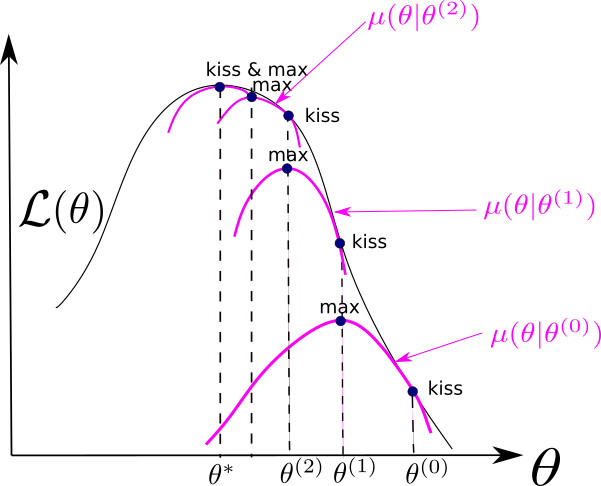
\includegraphics[width=3.7in]
{emax/minorize.png}
\caption{Function $\mu(\theta|\theta^{(t)})$
minorizes the function $\call(\theta)$.
Note that $\mu(\theta|\theta^{(t)})$
is always below
 $\call(\theta)$.
``max" indicates 
$\theta^{(t+1)}=
\argmax_\theta \mu(\theta|\theta^{(t)})$.
``kiss" indicates
 $\mu(\theta^{(t)}|\theta^{(t)})=
\call(\theta^{(t)})$. 
}
\label{fig-minorize}
\end{figure}



A function {\bf $\mu(\theta|\theta^{(t)})$ 
is said to minorize 
 a target
 function $\call(\theta)$}
iff for all $ \theta$ at fixed 
$\theta^{(t)}$,
it satisfies the
``$\mu\leq\call$ property"


\beq
\mu(\theta|\theta^{(t)})\leq
\call(\theta)
\;,
\eeq
and
the ``$\mu=\call$ property"

\beq
\mu(\theta^{(t)}|\theta^{(t)})=
\call(\theta^{(t)})
\;.
\eeq

We  {\bf recursively maximize a minorizing function} $\mu(\theta|\theta^{(t)})$
if we define a sequence $(\theta^{(t)})_{t=0, 1, \ldots}$
as follows:

\beq
\theta^{(t+1)}=\argmax_\theta \mu(\theta|\theta^{(t)})
\;.
\eeq

The sequence 
$(\call(\theta^{(t)}))_{t=0, 1, 2, \ldots}$
generated by 
recursively maximizing a minorizing function
must be nondecreasing:

\beq
\call(\theta^{(t+1)})\geq \mu(\theta^{(t+1)}
|\theta^{(t)})\geq
 \mu(\theta^{(t)}|\theta^{(t)}) 
= \call(\theta^{(t)})
\;.
\eeq

A {\bf
minorize-maximize (MM) algorithm}
is any algo that
specifies a
minorizing function $\mu(\theta|\theta^{(t)})$
for a particular target
 function $\call(\theta)$.
One can also define a 
{\bf majorize-minimize algo (also
called  MM)}
by inverting the inequalities throughout.


The EM algo is an MM algo.
Indeed, if we define 

\beq
\call(\theta)=\ln P(\vecx|\theta)
\eeq
and

\beq
\mu(\theta|\theta^{(t)})
=
Q(\theta|\theta^{(t)})
+
H(P(\ul{\vech}|\vecx, \theta^{(t)})
\;,
\eeq
then Eq.(\ref{eq-Q-decomposed})
establishes
the $\mu\leq \call$
and $\mu=\call$ properties
required of 
a minorizing function.

How an MM algo works 
is portrayed in Fig.\ref{fig-minorize}.


\section{Examples}

\subsection{Gaussian mixture}


$x[\sigma]\in \RR^d=S_\rvx$. $S_\rvh$ discrete and
not too large. $n_\rvh=|S_\rvh|$ is
number of Gaussians that we are 
going to fit the samples with.

Let
\beq
\theta = [w_h, \mu_h, \Sigma_h]_{h\in S_\rvh}
\;,
\eeq
where
$[w_h]_{h\in S_\rvh}$ is a probability
distribution of weights, and 
where $\mu_h\in\RR^d$
and $\Sigma_h\in\RR^{d\times d}$
are the mean value vector 
and covariance matrix of
a $d$-dimensional Gaussian distribution.

The TPMs, printed in blue,
for the nodes of Fig.\ref{fig-em-bnet},
for the special case
of a mixture of Gaussians, are as follows:

\beq\color{blue}
P(x[\sigma]\cond h[\sigma]\cond \theta)=
\caln_d(x[\sigma];\mu_{h[\sigma]}, \Sigma_{h[\sigma]})
\eeq

\beq\color{blue}
P(h[\sigma]\cond \theta)=w_{h[\sigma]}
\eeq

Note that

\beqa
P(x[\sigma]\cond \theta)&=&
\sum_h P(x[\sigma]\cond h[\sigma]=h, \theta)
P(h[\sigma]=h\cond\theta)
\\
&=&
\sum_hw_h\caln_d(x[\sigma];\mu_h, \Sigma_h)
\eeqa

\beqa
P(\vecx, \vech|\theta)&=&
\prod_\sigma \left[
w_{h[\sigma]}
\caln_d(x[\sigma];\mu_{h[\sigma]}, \Sigma_{h[\sigma]})
\right]
\\
&=&
\prod_\sigma\prod_h
\left[w_h
\caln_d(x[\sigma];\mu_h, \Sigma_h)\right]
^{\indi(h=h[\sigma])}
\eeqa

{\bf Old Faithful:}
See Wikipedia Ref.\cite{wiki-em}
for an animated
gif of a  classic example
of using EM to fit
samples with a Gaussian mixture.
Unfortunately,
could
not include it
here because pdflatex
does not support animated gifs. 
The gif shows samples in a 2 dimensional
space
(eruption time, delay time)
from the Old Faithful geyser.
In that example, $d=2$ and $n_\rvh=2$.
Two clusters of points
in a plane are fitted
by 
a mixture of 2 Gaussians.

{\bf K-means clustering} is often
presented as the main competitor
to EM for doing 
{\bf clustering (non-supervised
learning)}. In K-means clustering,
the sample points are 
split into $K$
mutually
disjoint sets $S_0, S_1, \ldots, S_{K-1}$. 
The algorithm is easy
to describe:
\begin{enumerate}
\item
Initialize by 
choosing  at random
$K$ data points $(\mu_k)_{k=0}^{K-1}$
called means or centroids
and placing $\mu_k$ in $S_k$
for all $k$.
 \item {\bf STEP 1:}
For each data point,
add it to the $S_k$
whose centroid $\mu_k$
is closest to it.
\item {\bf STEP 2:}
Recalculate the centroids.
Set $\mu_k$ equal to the mean value of set
$S_k$.
\item Repeat steps 1 and 2 until the
centroids stop changing 
by much.
\end{enumerate}
Step 1 is analogous
to the expectation step in EM,
and Step 2 to the maximization
step in EM ($\theta$
estimation versus 
$\mu_k$ estimation).
We won't say anything further
about K-means clustering because
it
isn't related to bnets in any 
way, and this is a book about bnets.
For more info about
K-means clustering, 
see Ref.\cite{wiki-k-means}.

\subsection{
Blood Genotypes and Phenotypes}

Notation:
$\vec{\rva}=
(\rva[\sigma])_{\sigma=0, 1, \ldots,nsam-1}
$, where $nsam$
is the number of samples.
Will
sometimes
denote
$a\sqsig$ by $a^\sqsig$.


Suppose
$\vec{\rvx}=
(\vec{\rvx}_0)
$ (i.e., just one component)

$\vec{\rvh}=
(\vec{\rvh}_0)
$ (i.e., just one component)



$\rvh[\sigma]\in S_\rvh=
\{AA, AO, BB, BO, OO, AB\}$ (the 6 blood genotypes)

$\rvx[\sigma]\in S_\rvx=
\{A,B,O,AB\}$ (the 4 blood phenotypes)

\begin{figure}[h!]
$$
\xymatrix{
\ul{\theta}\ar[d]\ar[dr]
\\
\rvx[\sigma]&\rvh[\sigma]\ar[l]
}$$
\caption{bnet 
for blood phenotypes $x\sqsig$
and genotypes $h\sqsig$.}
\label{fig-phenotypes}
\end{figure}

For the bnet of Fig.\ref{fig-phenotypes},
the TPMs, printed in blue, are:
\beq\color{blue}
P(h^\sqsig| \theta)=
\begin{array}{c|c}
&
\\\hline
AA&p_A^2
\\
AO&2p_Ap_O
\\
BB&p_B^2
\\
BO&2p_Bp_O
\\
OO&p_O^2
\\
AB&2p_Ap_B
\end{array}
\;,
\label{eq-pheno-ph}
\eeq
where $p_A+p_B+p_O=1$.


\beq\color{blue}
P(x^\sqsig\cond h^\sqsig, \theta)=
\begin{array}{l|llllll}
&AA&AO&BB&BO&OO&AB
\\\hline
A&1&1&0&0&0&0
\\
B&0&0&1&1&0&0
\\
O&0&0&0&0&1&0
\\
AB&0&0&0&0&0&1
\end{array}
\label{eq-pheno-pxbarh}
\eeq

\beq
\theta=(p_A, p_B)
\eeq

Multiplying the TPMs in
Eqs.(\ref{eq-pheno-ph}
and (\ref{eq-pheno-pxbarh}), we get
\beq
P(x^\sqsig\cond \theta)=
\begin{array}{l|l}
\\\hline
A&p_A^2+2p_Ap_O(=\pi_A)
\\
B&p_B^2+2p_Bp_O(=\pi_B)
\\
O&p_O^2(=\pi_O)
\\
AB&2p_Ap_B(=\pi_{AB})
\end{array}
\eeq


Note that 
\beqa
P(\vec{x}|\theta)
&=&
\prod_\sigma
P(x^\sqsig|\theta)
\\
&=&
(\pi_A)^{N_A}
(\pi_B)^{N_B}
(\pi_O)^{N_O}
(\pi_{AB})^{N_{AB}}
\;,
\eeqa 
where 
$N_x$ for $x\in S_\rvx=\{A, B, O, AB\}$
are
the counts from the data.
We can get estimates
for the parameters $p_A$ and $p_B$
right
here without doing EM.
Just note that

\beq
\hat{\pi}_x=
\frac{N_x}
{N_+}
\label{eq-quads-pi-x}
\eeq
for $x\in S_\rvx$,
where
$N_+=\sum_x N_x$. 
Eqs.(\ref{eq-quads-pi-x})
give  4 quadratic equations
that can be solved for the
parameters $p_A, p_B$
in terms of the observed 
counts $N_x$
for $x\in S_\rvx$.


If, instead,  you want to
find the optimum
parameters $p_A, p_B$
using EM, note that

\beqa
Q(\theta|\theta^{(t)})
&=&
\sum_{\vec{h}}
P(\vec{h}|\theta^{(t)})
\ln P(\vec{x}, \vec{h}|\theta)
\\
&=&
\sum_{\vec{h}}
\left[\prod_\sigma
P(h^\sqsig|\theta^{(t)})
\right]
\ln \left[
\prod_\sigma P(x^\sqsig, h^\sqsig |\theta)
\right]
\\
&=&\sum_\sigma 
\sum_{h^\sqsig}
P(h^\sqsig|\theta^{(t)})
\ln
 P(x^\sqsig, h^\sqsig |\theta)
\\
&=&\sum_\sigma 
\sum_{h^\sqsig}
P(h^\sqsig|\theta^{(t)})
[\ln
 P(x^\sqsig| h^\sqsig ,\theta)
+
\ln
 P(h^\sqsig |\theta)
]
\\
&=&nsam 
\sum_{h^\sqsig}
P(h^\sqsig|\theta^{(t)})
\ln
 P(h^\sqsig |\theta)
\;.
\eeqa

\subsection{Missing
 Data/Imputation}

The previous example
on blood genotypes and phenotypes
assumed no missing
data in compiling the
counts $N_x$. 
But what if there is missing
data? Can one
still apply
the EM algo in that case?
Yes! See Chapter \ref{ch-missing-d}.



\chapter{Frontdoor Adjustment Formula}
\label{ch-fdoor}
The frontdoor (FD) adjustment
formula is proven in
Chapter \ref{ch-do-calc}
from the rules of Do Calculus.
The goal 
of this chapter is
to give examples
of the use of that
theorem. We will restate
the theorem in this chapter,
sans proof.
There is no need
to understand the
theorem's
proof in order to use it.
However, you
will
need to skim Chapter \ref{ch-do-calc}
in order to familiarize 
yourself with
the notation used to state the 
theorem.
This chapter also assumes
that you are comfortable 
with the  rules 
for checking for d-separation. Those rules
are covered in Chapter \ref{ch-dsep}.


\fdoordef

\begin{claim} Frontdoor Adjustment Formula

\fdoorclaim

\end{claim}
\proof 
See Chapter \ref{ch-do-calc}.
\qed

\section{Examples}

\begin{enumerate}
\item
\beq
\xymatrix{
&*++[F-o]{\rvc}\ar[ld]\ar[rd]
\\
\rvx\ar[r]&\rvm\ar[r]&\rvy
}
\eeq
Can't satisfy backdoor
criterion because $\rvc$
unobserved so
can't condition on it 
to block
backdoor path $\rvx-\rvc-\rvy$.

If $\rvx.=\rvx,\rvm.=\rvm$ 
and $\rvy.=\rvy$,
then the FD criterion
is satisfied. In fact,

\beq
\xymatrix{\\
P(y|\cald \rvx=x)=
}
\xymatrix{
&\EE x'\ar[rd]
\\
x\ar[r]&\sum m\ar[r]&y
}
\eeq


\hrule\item
\beq
\xymatrix{
*++[F-o]{\rvz_1}\ar[d]\ar[dr]
&&
*++[F-o]{\rvz_2}\ar[d]\ar[dl]
\\
*++[F-o]{\rvw_1}\ar[d]
&\rvc\ar[ld]\ar[rd]
&*++[F-o]{\rvw_2}\ar[d]
\\
\rvx\ar[r]&\rvm\ar[r]&\rvy
}
\eeq
Can't satisfy backdoor
criterion because 
to block 
backdoor path $\rvx-\rvc-\rvy$,
need to condition on $\rvc$
but if this is true, 
then long
path 
$\rvx-\rvw_1-\rvz_1-\rvc-\rvz_2-\rvw_2-\rvy$
becomes unblocked.

If $\rvx.=\rvx,\rvm.=\rvm$ 
and $\rvy.=\rvy$,
then the FD criterion
is satisfied. In fact,

\beqa
\xymatrix{\\
P(y|\cald\rvx=x)=
}
&&
\xymatrix{
*++[F-o]{\EE z_1}\ar[d]\ar[dr]
&&
*++[F-o]{\EE z_2}\ar[d]\ar[dl]
\\
*++[F-o]{\sum w_1}
&\sum c\ar[rd]
&*++[F-o]{\sum w_2}\ar[d]
\\
x\ar[r]&\sum m\ar[r]&y
}
\\
&=&
\xymatrix{
*++[F-o]{\EE x'}\ar[d]\ar[dr]
&&
*++[F-o]{\EE x''}\ar[d]\ar[dl]
\\
*++[F-o]{\sum w_1}
&\sum c\ar[rd]
&*++[F-o]{\sum w_2}\ar[d]
\\
x\ar[r]&\sum m\ar[r]&y
}
\\
&=&
\xymatrix{
&\EE x'\ar[rd]
&
\\
x\ar[r]&\sum m\ar[r]&y
}
\eeqa


\end{enumerate}
\chapter{Generative Adversarial Networks
 (GANs)}
%\begin{refsection}

\begin{figure}[h!]
\centering
\includegraphics[width=6in]{gan/gan.png}
\caption{Generative Adversarial  Network (GAN)} 
\label{fig-gan}
\end{figure}

\begin{figure}[h!]
\centering
\includegraphics[width=6in]{gan/gan-detail.png}
\caption{Discriminator node $\ul{V}$ in Fig.\ref{fig-gan} can be
split into 3 nodes $\vec{\rvc}$, $\vec{\rvd}$ and $\ul{V}$.} 
\label{fig-gan-detail}
\end{figure}

Original GAN, 
Ref.\cite{gf2014}(2014). 

Generator $G$ (counterfeiter) generates samples $\vecf$ of fake money and submits them to Discriminator $D$ (Treasury agent). $D$ also gets samples $\vecr$ of real money. $D$ submits veredict $V\in [0,1]$. $G$ depends on parameter $\theta_G$ and $D$ on parameter $\theta_D$. Veredict $V$ and initial $\theta_G, \theta_D$ are used to get new parameters $\theta'_G, \theta'_D$.Process is repeated (Dynamical Bayesian Network) until saddle point in $V(\theta_G, \theta_D)$ is reached. $D$ makes $G$ better and vice versa.  Zero-sum game between $D$ and $G$.



Let $\cald$ be the domain of $D(\cdot, \theta_D)$. Assume that for any $x\in \cald$,

\beq
0\leq D(x,\theta_D)\leq 1
\;.
\eeq
For any $S\subset\cald$, define

\beq
\sum_{x\in S}D(x,\theta_D)=\lam(S,\theta_D)
\;.
\eeq


 In general, 
$G(\cdot,\theta_G)$ need not be real valued. 

Assume that for every $u\in S_\rvu$,
 $G(u,\theta_G)=f\in S_\rvf\subset \cald$. Define
\beq
\ol{D}(f,\theta_D)=1-D(f,\theta_D)
\;.
\eeq
Note that

\beq
0\leq\ol{D}(f,\theta_D)\leq 1
\;.
\eeq

Define:

\beq
V(\theta_G, \theta_D) =
\sum_{r}P(r)
\ln D(r, \theta_D)
+ \sum_{u}P(u)\ln
\ol{D}(G(u,\theta_G),\theta_D)
\;.	
\eeq

We want the first variation of $V(\theta_G, \theta_D)$ to vanish.




\beq
\delta V(\theta_G, \theta_D)=0
\;.
\eeq
This implies

\beq
 \partial_{\theta_G}V(\theta_G, \theta_D)=
 \partial_{\theta_D}V(\theta_G, \theta_D)=0
\;
\eeq
and

\beq
V_{opt}=\min_{\theta_G}\max_{\theta_D} V(\theta_G, \theta_D)
\;.
\eeq

Node TPMs
for Figs.\ref{fig-gan} and \ref{fig-gan-detail} 
are
given next in blue:

\beq\color{blue}
P(\theta_G)=\;{\rm given}
\eeq

\beq\color{blue}
P(\theta_D)=\;{\rm given}
\eeq


\beq\color{blue}
P(\vecu)=\prod_i P(u[i])  \;\;{\rm (usually \;uniform\; distribution)}
\eeq

\beq\color{blue}
P(\vecr)=\prod_i P(r[i])
\eeq


\beq\color{blue}
P(f[i]\cond \vecu, \theta_G)= \delta[f[i], G(u[i],\theta_G)]
\eeq

\beq\color{blue}
P(c[i]\cond \vecf, \theta_D) = \delta(c[i], \ol{D}(f[i], \theta_D))
\eeq

\beq\color{blue}
P(d[j]\cond \vecr, \theta_D)= \delta(d[j], D(r[j], \theta_D))
\eeq




\beq\color{blue}
P(V| \vecd,  \vecc)=
\delta(V, \frac{1}{N}\ln \prod_{i,j}(c[i]d[j]))
\eeq
where $N=nsam(\vecr)nsam(\vecu)$.


Let $\eta_G, \eta_D> 0$. Maximize $V$ wrt $\theta_D$, and
minimize it wrt $\theta_G$.

\beq\color{blue}
P(\theta'_G|V,\theta_G )=
\delta(\theta'_G, \theta_G - \eta_G 
\partial_{\theta_G}V)
\eeq

\beq\color{blue}
P(\theta'_D|V,\theta_D )=
\delta(\theta'_D, \theta_D + \eta_D 
\partial_{\theta_D}V)
\eeq

\hrule
\begin{figure}[h!]
\centering
\includegraphics[width=2in]{gan/gan-emulate.png}
\caption{GAN, Constraining Bayesian Network}
\label{fig-gan-emulate} 
\end{figure}

Constraining B net given in Fig.\ref{fig-gan-emulate}. It adds 2 new nodes, namely $\ul{\vec{U}}$ and $\ul{\vec{R}}$, to  the bnet of Fig.\ref{fig-gan}. The purpose of these 2  barren (childrenless) nodes is to constrain certain functions to be probability distributions.

Node TPMs for the 2 new nodes given next in blue.


\beq\color{blue}
P(U[i]\cond \theta_G)= 
\frac{\ol{D}(G(U[i],\theta_G),\theta_D))}
{\ol{\lam}(\theta_G, \theta_D)}
\eeq
where  $S_{\ul{U[i]}}=S_\rvu$ and $\ol{\lam}(\theta_G, \theta_D)=\sum_u\ol{D}(G(u, \theta_G), \theta_D))$.

\beq\color{blue}
P(R[i]\cond \theta_G, \theta_D)= \frac{D(R[i], \theta_D)}{\lam(\theta_D)}
\eeq
where $S_{\ul{R[i]}}=S_\rvr$ and  $\lam(\theta_D)=\sum_r D(r, \theta_D)$.


\beq\color{blue}
P(V| \vecu,  \vecr)=
\delta(V, \frac{1}{N}\ln \prod_{i,j}(
P(\ul{R[i]}=r[i]\cond \theta_G, \theta_D)P(\ul{U[i]}=u[j]\cond \theta_G)))
\eeq
where $N=nsam(\vecr)nsam(\vecu)$.


$\call=$ likelihood
\beqa
\call&=&
P(\vecr, \vecu| \theta_G, \theta_D)\\
&=&
\prod_{i,j}\left[
 \frac{D(r[i], \theta_D)}{\lam(\theta_D)}
\frac{\ol{D}(G(u[j],\theta_G),\theta_D))}
{\ol{\lam}(\theta_G, \theta_D)}
\right]
\eeqa

\beq
\ln \call = N[V(\theta_G, \theta_D)
-\ln \lam(\theta_D)-\ln \ol{\lam}(\theta_G, \theta_D)]
\eeq



%\printbibliography[heading=subbibliography]
%\end{refsection}


 
\chapter{Gaussian Nodes with
 Linear Dependence on Parents}
\label{ch-gauss-lin}

Bnet nodes
that 
have a Gaussian TPM
with a linear dependence
on their parent nodes (GLP)
are a very
popular way 
of modeling continuous
nodes of bnets.
A 
convenient
aspect of them
is that their
parents can be discrete
or continuous nodes,
and their
children can be discrete
or continuous nodes too.
Also,
they can be learned 
easily
from the data
because
their
parameters
can
be expressed in terms of
two node
covariances.
For these reasons, 
they are commonly
used when 
doing
structure learning of 
bnets 
with continuous nodes (see Chapter \ref{ch-struc-learn}).

\begin{figure}[h!]
$$\xymatrix{
\rvy
&\rvx_1\ar[l]
\\
&\rvx_2\ar[lu]
\\
&\rvx_3\ar[luu]
}$$
\caption{GLP node
$\rvy$ with 3 parent nodes $\rvx^3
=
(\rvx_1, \rvx_2, \rvx_3)$.}
\label{fig-glp-3}
\end{figure}

Recall our
notation
for a Gaussian distribution:
\beq
\caln(x;\mu, \sigma^2)
=
\frac{1}{\sigma\sqrt{2\pi}}
e^{\frac{-(x-\mu)^2}{2\sigma^2}}
\;,
\eeq
where 
$x, \mu\in \RR$
and $\sigma>0$.

A GLP node $\rvy$ with 
$n$ parents
 $\rvx^n=(\rvx_1, \rvx_2, \ldots, \rvx_n)$
has the following TPM:
\beq\color{blue}
P(y|x^n)=
\caln(y; \beta_0 + 
\beta^{nT}x^n, \sigma^2)
\eeq
where $\rvy, \beta_0, \in\RR$
and $\sigma^2>0$, and where
$\rvx^n, \beta^n\in \RR^n$ 
are **column vectors**.
The $T$ 
in $\beta^{nT}$ stands for transpose.
Any $\rvx_i$
can have
a discrete
set of states
as long as they are real
valued and ordinal (ordered by size).
 Fig.\ref{fig-glp-3}
shows a diagrammatic
representation
of a GLP node with 3 parents.

Note that as $\sigma\rarrow 0$,
a GLP node becomes 
deterministic.
In fact,
it
becomes a neural
net node
with a linear activation function.


An equivalent
way of defining a GLP node $\rvy$
is in terms of a random variable
equation expressing
$\rvy$ as a hyperplane
function of the parents $\rvx^n$
plus a  Gaussian noise variable.
Define a curve-fit $\HAT{\rvy}$
of a \qt{true value}
$\rvy$ by
\begin{subequations}
\beq
\HAT{\rvy}=\beta_0 + \beta^{nT}\rvx^n
\eeq
and

\beq
\rvy=\HAT{\rvy}+\ul{\eps}
\eeq
where the residual $\ul{\eps}$
satisfies 

\beq
P(\eps)=\caln(\eps; 0, \sigma^2)
\eeq
and


\beq
\av{\rvx^n, \ul{\eps}}
=0
\;.
\eeq
\end{subequations}

The notation $\av{\rvx, \rvy}$
for the covariance
of random variables
$\rvx$ and $\rvy$
is explained
in Chapter \ref{ch-conventions}.

\begin{claim}
The
parameters of
a GLP node
can be expressed
in terms of 2-node
covariances.
Specifically,

\beq
\beta^n=
\av{\rvx^n, \rvx^{nT}}^{-1}
\av{\rvy, \rvx^n}
\eeq

\beq
\beta_0=
\av{\rvy}-
\beta^{nT}\av{\rvx^n}
\eeq

\beq
\sigma^2
=
\av{\rvy, \rvy}
-\beta^{nT}
\av{\rvx^n, \rvy}
\eeq
\end{claim}
\proof

Note that $\av{\rvx^n, \rvx^{nT}}^T
=\av{\rvx^n, \rvx^{nT}}$
and 
$\av{\rvy, \rvx^{nT}}^T
=\av{\rvy, \rvx^n}$.


\beq
\av{\rvy, \rvx^{nT}}
=
\beta^{nT}\av{\rvx^n, \rvx^{nT}}
\eeq

\beq
\av{\rvy, \rvx^n}=
\av{\rvx^n, \rvx^{nT}}\beta^n
\eeq

\beq
\beta^n
=
\av{\rvx^n, \rvx^{nT}}^{-1}
\av{\rvy, \rvx^n}
\eeq

\beq
\av{\rvy}=
\beta_0 + 
\beta^{nT}\av{\rvx^n}
\eeq

\beqa
\av{\rvy, \rvy}
&=&
\av{
\beta_0 + \beta^{nT}\rvx^n +
\ul{\eps},
\rvy}
\\
&=&
\beta^{nT}\av{\rvx^n,
\rvy}
+
\sigma^2
\eeqa
\qed

\hrule
Let  D=Discrete, GLP=Gaussian with  Linear
 dependence in Parents

The following arrows are possible
in a bnet.

\begin{itemize}
\item $GLP\larrow GLP$
\item $GLP\larrow D$

Pass to GLP a separate
set of regression
coefficients $\beta_0, \beta^n$
and variance $\sigma^2$
for each state 
of D. If D is called $\rvd$,
let
\beq\color{blue}
P(y|(x^n)_d, d)=
\caln(y; (\beta_0)_d + 
(\beta^{nT})_d (x^n)_d, \sigma_d^2)
\eeq
for each $d\in S_{\rvd}$.

\item $D\larrow GLP$

If D expects
a continuous parent,
no need to preprocess GLP output.
If D expects a discrete parent,
break
the interval $[a,b]$
that
contains
most of
the range
of the GLP node into
sub-intervals and 
assign a discrete label
to each subinterval.
\item $D\larrow D$
\end{itemize}
\chapter{Hidden Markov Model}\label{ch-hmm}

A Hidden Markov Model (HMM) is
 a  generalization of a
Kalman Filter (KF). KFs 
are discussed 
in Chapter \ref{ch-kalman}. The
bnets of HHMs and KFs
bnets are the same.
The only difference is that a
KF assumes
special node
transition matrices.

See Wikipedia article 
Ref.\cite{wiki-hmm} to learn 
about the history 
and many uses of HMMs. This
chapter is based on
Ref.\cite{nuel}.

\begin{figure}[h!]
\centering
$$\xymatrix{
\rvx_0\ar[d]\ar[r]&
\rvx_1\ar[d]\ar[r]&
\rvx_2\ar[d]\ar[r]&
\rvx_3\ar[d]\\
\rvv_0&
\rvv_1&
\rvv_2&
\rvv_3
}$$
\caption{HMM bnet
with $n=4$.}
\label{fig-hmm}
\end{figure}

Suppose 

$\rvv^n=(\rvv_0, \rvv_1, 
\ldots, \rvv_{n-1})$
are $n$ visible nodes that
are measured,
and 

$\rvx^n=(\rvx_0, \rvx_1, 
\ldots, \rvx_{n-1})$
are the $n$ hidden, unmeasurable 
state nodes of a system
that is being monitored.



For the bnet of Fig.\ref{fig-hmm},
one has
\beq
P(x^n, v^n)=\prod_{i=0}^{n-1}
P(x_i|x_{i-1})P(v_i|x_i)
\;,
\eeq
where $x_{-1}=0$.

Let
$x_{<i} =(x_0, x_1, \dots, x_{i-1})$.

For $i=0,1, \dots, n-1$, define

$\calf_i$=future measurements probability

\beq
\calf_i(x_i)=
P(v_{> i}|x_i)
\eeq

$\ol{\calf}_i$= 
past and present measurements  probability

\beq
\ol{\calf}_i(x_i)=
P(v_{<i},v_i, x_i)
\eeq

$\lam_i$=
present measurement probability

\beq
\lam_i(x_i)=
P(v_i|x_i)
\eeq

$\calf_i$, $\ol{\calf}_i$
and $\lam_i$ 
can be represented graphically
as follows:

\beq
\begin{array}{cc}
\calf_i(x_i)
=
\frac{1}
{P(x_i)}
\sum_{x_{>i}}&
\xymatrix{
x_i\ar[r]
&x_{>i}\ar[d]
\\
&v_{>i}
}
\end{array}
\eeq

\beq
\begin{array}{cc}
\ol{\calf}_i(x_i)
=
\sum_{x_{<i}}&
\xymatrix{
x_{<i}\ar[r]\ar[d]
&x_i\ar[d]
\\
v_{<i}&v_i
}
\end{array}
\eeq

\beq
\begin{array}{cc}
\lam_i(x_i)
=
\frac{1}
{P(x_i)}
&
\xymatrix{
x_i\ar[d]
\\
v_{i}
}
\end{array}
\eeq

\begin{claim}
For $i\geq 0$, 
\beq
P(x_i, v^n)=
\ol{\calf}_i(x_i)\calf_i(x_i)
\;.
\eeq
For $i>0$,

\beq
P(x_{i-1},x_i, v^n)=
 \ol{\calf}_{i-1}(x_{i-1})
\lam_i(x_i)P(x_i|x_{i-1})\calf_i(x_i)
\;.
\eeq


\end{claim}
\proof

\beqa
P(x_i,v^n)
&=&
\sum_{x_{< i}}\sum_{x_{> i}}
P(x^n, v^n)
\\
&=&
\sum_{x_{< i}}\sum_{x_{> i}}
P(x^n, v^n|x_i)P(x_i)
\\
&=&
\sum_{x_{< i}}\sum_{x_{> i}}
P(x_{< i}, v_{< i}, v_i|x_i)
P(x_{>i}, v_{>  i}|x_i)
P(x_i)
\\
&=&
P( v_{< i}, v_i|x_i)
P(v_{>  i}|x_i)
P(x_i)
\\
&=&
\ol{\calf}_i(x_i)\calf_i(x_i)
\eeqa

\beqa
P(x_{i-1},x_i,v^n)
&=&
\sum_{x_{< i-1}}\sum_{x_{>i}}
P(x^n, v^n)
\\
&=&
\sum_{x_{< i-1}}\sum_{x_{>i}}
P(x^n, v^n|x_{i-1}, x_i)P(x_{i-1}, x_i)
\\
&=&
\sum_{x_{< i-1}}\sum_{x_{>i}}
P(x_{<i-1}, v_{<i-1}, v_{i-1}|x_{i-1})
P(v_i|x_i)
P(x_{i-1}, x_i)
P(x_{>  i}, v_{> i}|x_i)
\\
&=&
P( v_{<i-1}, v_{i-1}|x_{i-1})
P(v_i|x_i)
P(x_{i-1}, x_i)
P( v_{> i}|x_i)
\\&=&
 \ol{\calf}_{i-1}(x_{i-1})
\lam_i(x_i)
P(x_i|x_{i-1})
\calf_i(x_i)
\eeqa
\qed

\begin{claim}
For $i>0$, $\calf_i$ and
$\ol{\calf}_i$ can be calculated 
recursively as follows:


\beq
\ol{\calf}_i(x_{i})
=
\sum_{x_{i-1}}
\ol{\calf}_{i-1}(x_{i-1})
\lam_i(x_i)
P(x_i|x_{i-1})
\eeq

\beq
\calf_{ i-1}(x_{i-1})
=
\sum_{x_i}\lam_i(x_i)
P(x_i|x_{i-1})
\calf_i(x_{i})
\eeq

\end{claim}
\proof

\beqa
\ol{\calf}_i(x_i)\calf_i(x_i)
&=&
P(x_i, v^n)\\
&=&
\sum_{x_{i-1}}P(x_{i-1},x_i, 
v^n)\\
&=&\sum_{x_{i-1}}
\ol{\calf}_{i-1}(x_{i-1})
\lam_i(x_i)
P(x_i|x_{i-1})\calf_i(x_i)
\eeqa

\beqa
\ol{\calf}_{i-1}(x_{i-1}
)\calf_{i-1}(x_{i-1})
&=&
P(x_{i-1}, v^n)\\
&=&
\sum_{x_i}P(x_{i-1},x_i, 
v^n)\\
&=&\sum_{x_i}
\ol{\calf}_{i-1}(x_{i-1})
\lam_i(x_i)
P(x_i|x_{i-1})\calf_i(x_i)
\eeqa
\qed

\begin{claim}
\beq
P(x_i|x_{i-1}, v^n)=
\frac{\lam_i(x_i)\calf_{i}(x_i)}
{\calf_{i-1}(x_{i-1})}P(x_i|x_{i-1})
\eeq

\beq
P(x_{i-1}|x_i, v^n)=
\frac{\lam_i(x_i)\ol{\calf}_{i-1}(x_{i-1})}
{\ol{\calf}_i(x_{i})}P(x_i|x_{i-1})
\label{eq-update-2}
\eeq
\end{claim}
\proof
\beqa
P(x_i|x_{i-1}, v^n)&=&
\frac{P(x_{i-1}, x_i, v^n)}
{P(x_{i-1}, v^n)}
\\&=&
\frac{
\ol{\calf}_{i-1}(x_{i-1})
\lam_i(x_i)
P(x_i|x_{i-1})\calf_i(x_i)
}{
\ol{\calf}_{i-1}
(x_{i-1})\calf_{i-1}(x_{i-1})
}
\eeqa
Analogous 
proof for Eq.(\ref{eq-update-2}).
\qed


\chapter{Influence Diagrams \& Utility Nodes}
\label{ch-inf-dia}

Influence diagrams are
just arbitrary bnets
enhanced with a 
new kind of node called an utility node.
The rest
of this brief chapter  will 
be devoted to discussing utility nodes.

Suppose $U(x)$ is a deterministic 
function $U:S_\rvx\rarrow \RR$
called the {\bf utility function}.
Then the {\bf expected utility}
is defined as


\beqa
E_\rvU[\rvU]&=&\sum_UP(U)U
\\
&=&\sum_x\sum_U
\underbrace{P(U|x)}_
{\delta[U, U(x)]}P(x)U
\\
&=&
\sum_xP(x)U(x)
\;.
\eeqa

An {\bf utility node}
can be
understood
as a node
composed of 3 simpler bnet nodes.
This
is illustrated in Fig.\ref{fig-util-node}.

\begin{figure}[h!]
\centering
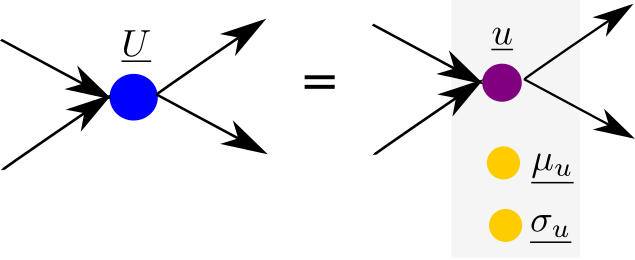
\includegraphics[width=3.5in]
{inf-dia/util-node.png}
\caption{An utility node
can be
understood
as a node 
composed of 3 simpler bnet nodes.} 
\label{fig-util-node}
\end{figure}

The TPMs,
printed in blue,
for the bnet Fig.\ref{fig-util-node},
are as follows:

\beq\color{blue}
P(U|pa(U))=\delta[U, U(pa(U))]
\;,
\eeq
where if $U:S_\rvx\rarrow \RR$,
then $\rvx=pa(\rvU)$.

\beq\color{blue}
P(u|pa(U))=
\delta[u, U(pa(U))]
\eeq

Node $\ul{\mu}_u$
calculates the
expected value (mean value) of $\rvu$:

\beq\color{blue}
P(\mu_u)=\delta(\mu_u,
E_{\rvu}[\rvu])
\eeq

Node $\ul{\sigma}_u$
calculates the
standard deviation of $\rvu$:
\beq\color{blue}
P(\sigma_u)=\delta(\sigma_U,
\sqrt{
E_{\rvu}[
(\rvu-E_{\rvu}[\rvu])^2]})
\eeq

Note that in order to
calculate expected values,
it is necessary that
$\rvU, \rvu\in \RR$. Note that
nodes $\rvu$, $\ul{\mu}_u$, $\ul{\sigma}_u$
must all 3 have access
to the 
TPM
$P(U|pa(U))$ of node $\rvU$.
In fact, in order  to
calculate $E_\rvu[\cdot]$,
it is necessary for
nodes $\ul{\mu}_u$ and 
 $\ul{\sigma}_u$
to have access not just to 
$P(U|pa(U))$ but also to
$P(pa(U))$.

See Fig.\ref{fig-util-merge}.
An influence
diagram may have multiple
utility nodes ($\rvU_1$ and
$\rvU_2$ in Fig.\ref{fig-util-merge}).
Then one can define a merging
utility node $\rvU$ that sums
the values of
all the other utility 
nodes.

\begin{figure}[h!]
\centering
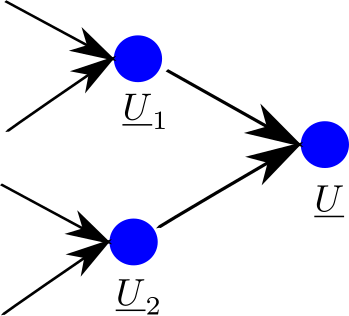
\includegraphics[width=1.5in]
{inf-dia/util-merge.png}
\caption{An influence
diagram may have multiple
utility nodes, say $\rvU_1$ and
$\rvU_2$. Then
one can define an
utility node $\rvU=\rvU_1 + \rvU_2$. } 
\label{fig-util-merge}
\end{figure}

For the node $\rvU$ of 
Fig.\ref{fig-util-merge},
\beq\color{blue}
P(U|U_1, U_2)=\delta(U,U_1 + U_2)
\eeq
%
\chapter{IN PROGRESS: Generative Adversarial Networks, Ensemble GANs}
\begin{refsection}
Bayesian GAN, 
 Ref.\cite{wilson2017} (2017)

Replace $\theta_a$ by $\vtheta_a$ and 
$\theta'_a$ by $\vtheta'_a$ for $a=G,D$



\beq
\delta V(\vtheta_G, \vtheta_D)=0
\eeq

\beq
 \partial_{\vtheta_G}V(\vtheta_G, \vtheta_D)=
 \partial_{\vtheta_D}V(\vtheta_G, \vtheta_D)=0
\eeq

\beq
V_{opt}=\min_{\vtheta_G}\max_{\vtheta_D} V(\vtheta_G, \vtheta_D)
\eeq

\beq
P(\vtheta_G)=\prod_i P(\theta_G[i])
\eeq

\beq
P(\vtheta_D)=\prod_i P(\theta_D[i])
\eeq


\beq
P(\vecu)=\prod_i P(u[i])
\eeq

\beq
P(\vecr)=\prod_i P(r[i])
\eeq


\beq
P(f[i]|\vecu, \vtheta_G)= \prod_i\delta[f[i], G(u[i],\vtheta_G)]
\eeq

\beq
P(c[i]|\vecf, \vtheta_D) = \delta(c[i], \ol{D}(f[i], \vtheta_D))
\eeq

\beq
P(d[j]|\vecr, \vtheta_D)= \delta(d[j], D(r[j], \vtheta_D))
\eeq


\beq
P(V| \vecd,  \vecc)=
\delta(V, \frac{1}{N}\ln \prod_{i,j}(c[i]d[j]))
\eeq
where $N=nsam(\rvr)nsam(\rvu)$







$\eta_G, \eta_D> 0$, maximize wrt $\theta_D$, 
minimize wrt $\theta_G$
\beq
P(\theta'_G|V,\vtheta_G )=
\delta(\vtheta'_G, \vtheta_G - \eta_G 
\partial_{\vtheta_G}V)
\eeq

\beq
P(\theta'_D|V,\vtheta_D )=
\delta(\vtheta'_D, \vtheta_D + \eta_D 
\partial_{\vtheta_D}V)
\eeq


\hrule
Emulated B net

\beq
P(\vtheta_G)=\;\prod_i P(\theta_G[i])
\eeq

\beq
P(\vtheta_D)=\;\prod_i P(\theta_D[i])
\eeq


\beq
P(u[i]|\vtheta_G, \vtheta_D)=  
\ol{D}(G(u[i],\vtheta_G), \vtheta_D)
\eeq


\beq
P(r[i]|\vtheta_D)=  
D(r[i], \vtheta_D)
\eeq

\beq
P(V| \vecd,  \vecc)=
\delta(V, \prod_{i,j,a,b}(u[i]r[j]\theta_G[a]\theta_D[b]))
\eeq



$\eta_G, \eta_D > 0$, maximize wrt $\theta_D$, 
minimize wrt $\theta_G$
\beq
P(\vtheta'_G|V,\vtheta_G )=
\prod_i \delta(\theta'_G[i], \theta_G[i] - \eta_G 
\partial_{\theta_G[i]}\ln V)
\eeq

\beq
P(\vtheta'_D|V,\vtheta_D )=\prod_i
\delta(\theta'_D[i], \theta_D[i] + \eta_D 
\partial_{\theta_D[i]}\ln V)
\eeq

\beq
P(\vecr, \vecu, \vtheta_G, \vtheta_D)=
\prod_{i,j,a,b}
\left\{
P(\theta_G[a])P(\theta_D[b])\\
 \frac{D(r[i], \theta_D[b])}{\lam(\theta_D[b])}
\frac{\ol{D}(G(u[j],\theta_G[a]),\theta_D[b]))}
{\ol{\lam}(\theta_G[a], \theta_D[b])}
\right\}
\eeq


$N=nsam(\vecr)nsam(\vecu)
nsam(\vtheta_G)nsam(\vtheta_D)$

\beq
\ln P(\vecr, \vecu, \vtheta_G, \vtheta_D) =
N\left\{
\begin{array}{l}
-H(P_{\ul{\theta}_D})+ \sum_{r,\theta_D}P(r)P(\theta_D)
\ln \frac{D(r, \theta_D)}{\lam(\theta_D)}
\\
-H(P_{\ul{\theta}_G})+ \sum_{u,\theta_G,\theta_D}P(u)
P(\theta_G)P(\theta_D)\ln
\frac{\ol{D}(G(u,\theta_G),\theta_D)}{\ol{\lam}(\theta_G, \theta_D)}
\end{array}
\right.
\eeq

\beq
\ln P(\vecr, \vecu) =
N\left\{
\begin{array}{l}
 \sum_{r}P(r)
\ln \sum_{\theta_D}P(\theta_D)\frac{D(r, \theta_D)}{\lam(\theta_D)}
\\
+ \sum_{u}P(u)
\ln \sum_{\theta_D, \theta_G}
P(\theta_G)P(\theta_D)
\frac{\ol{D}(G(u,\theta_G),\theta_D)}{\ol{\lam}(\theta_G, \theta_D)}
\end{array}
\right.
\eeq

\beqa
V(\vtheta_G, \vtheta_D) &=&\frac{1}{N} \ln P(\vtheta_G, \vtheta_D|\vecr,\vecu,)\\&=&
\frac{1}{N} [
\ln P(\vecr,\vecu,\vtheta_G, \vtheta_D)
-\ln P(\vecr,\vecu)]
\eeqa



\printbibliography[heading=subbibliography]
\end{refsection}

\chapter{Junction Tree Algorithm}
\label{ch-junc-tree}
The Junction Tree (JT)
algorithm
is an algo
for evaluating
exact marginals
of a bnet, 
including cases in which
some nodes are fixed to a single state.
(fixed nodes
are called the a priori evidence.)

The JT algo
starts by  
clustering
the loops of a bnet into bigger nodes
so as  to
transform the bnet into a tree bnet.
Then it applies
Pearl Belief Propagation (see
Chapter \ref{ch-mp}) to the ensuing tree.
The first breakthrough 
paper to achieve this agenda in full
was Ref.\cite{lauritzen1988}
by Lauritzen, and Spiegelhalter in 1988.
See the Wikipedia article 
Ref.\cite{wiki-junc-tree}
for more info and
 references on the JT algorithm. 

I won't describe
the JT algo
any further here,
because it would take too
long for this brief book
to give a complete treatment
of it, including the mathematical proofs.
If all you want to do is to
code the JT algo, without
delving into the mathematical theorems
and proofs behind it, I 
strongly recommend 
Ref.\cite{huang1996}.
Ref.\cite{huang1996} is 
an excellent cookbook
for programmers of the JT algo. My
open source  
program QuantumFog (see Ref.\cite{qfog})
implements the
JT algo in Python, 
following the recipe of
Ref.\cite{huang1996}.
\chapter{Kalman Filter}\label{ch-kalman}

A Kalman Filter is a special case of a
Hidden Markov Model. HMMs are
 discussed in Chapter \ref{ch-hmm}.

\begin{figure}[h!]
\centering
$$\xymatrix{
\rvx_0\ar[d]\ar[r]&
\rvx_1\ar[d]\ar[r]&
\rvx_2\ar[d]\ar[r]&
\rvx_3\ar[d]\\
\rvz_0&
\rvz_1&
\rvz_2&
\rvz_3
}$$
\caption{Kalman Filter bnet with $T=4$.}
\label{fig-kal}
\end{figure}

Let $t=0, 1, 2, \dots , T-1$.

$\rvx_t\in S_\rvx$ are
random variables that represent
the hidden (unobserved) true
state of the system.

$\rvz_t\in S_\rvz$ are 
random variables that represent
the measured (observed) state of the system.


The Kalman Filter bnet Fig.\ref{fig-kal}
has the following
node TPMs,
printed in blue:


\beq\color{blue}
P(x_t|x_{t-1})=
\caln(x_t;F_tx_{t-1} + B_tu_t, Q_t)\;,
\eeq
where $F_t, Q_t, B_t, u_t$
are given. $P(x_t|x_{t-1})$ becomes $P(x_t)$
for $t=0$.

\beq\color{blue}
P(z_t|x_t)=
\caln(z_t; H_tx_t, R_t)
\;,
\eeq
where $H_t, R_t$ are given.

Define

\beq
\rvZ_t= (\rvz_{t'})_{t'\leq t}
\;.
\eeq
Define $\hat{x}_t$ and $P_t$ by

\beq
P(x_t|Z_t)=
\caln(x_t; \hat{x}_t, P_t)
\;.
\eeq
\hrule
\medskip
\noindent
Problem: Find $\hat{x}_t$ and $P_t$
in terms of 
\begin{enumerate}
\item
 current (at time $t$)
 given values of
$F,Q,H,R,
 B ,u$
\item
 current (at time $t$)
observed  value of 
$z$
\item
prior (previous)
value (at time $t-1$) of $\hat{x}$
and $P$.
\end{enumerate}
See Fig.\ref{fig-kal-plus}.
For that figure,

\beq \color{blue}
P(\hat{x}_t, P_t | z_t,
\hat{x}_{t-1}, P_{t-1})
=\delta(\hat{x}_t,?)
\delta(P_t, ?)
\;.
\eeq

\begin{figure}[h!]
\centering
$$\xymatrix{
\rvx_0\ar[d]\ar[r]&
\rvx_1\ar[d]\ar[r]&
\rvx_2\ar[d]\ar[r]&
\rvx_3\\
\rvz_0\ar[d]&
\rvz_1\ar[d]&
\rvz_2\ar[d]&
\rvz_3\\
\ul{\hat{x}}_0, 
\ul{P}_0\ar[r]&
\ul{\hat{x}}_1, 
\ul{P}_1\ar[r]&
\ul{\hat{x}}_2, 
\ul{P}_2\ar[r]&
\ul{\hat{x}}_3, 
\ul{P}_3
}$$
\caption{Kalman Filter bnet
with deterministic nodes for 
$\hat{x}_t, P_t$.}
\label{fig-kal-plus}
\end{figure}

\hrule \noindent
Solution copied from Wikipedia Ref.\cite{wiki-kalman}:


Define $\eta_{t|t}=\eta_t$ for 
$\eta=\hat{x}, P$.

\begin{itemize}
\item{\bf Predict}

Predicted (a priori) state estimate
\beq
\hat{\mymathbf{x}}_{t\mid t-1} =
 \mymathbf{F}_t
\hat{\mymathbf{x}}_{t-1\mid t-1}
 + \mymathbf{B}_t \mymathbf{u}_{t}
\eeq

Predicted (a priori) estimate covariance
\beq
\mymathbf{P}_{t\mid t-1} =
 \mymathbf{F}_t 
\mymathbf{P}_{t-1\mid t-1}
 \mymathbf{F}_t^\textsf{T} +
 \mymathbf{Q}_t
\eeq

\item{\bf Update}

Innovation (or measurement 
pre-fit residual)
\beq
\tilde{\mymathbf{y}}_{t|t-1}= 
\mymathbf{z}_t - 
\mymathbf{H}_t\hat{\mymathbf{x}}_{t\mid t-1}
\eeq

Innovation (or pre-fit residual)
 covariance
\beq
\mymathbf{S}_t = \mymathbf{H}_t 
\mymathbf{P}_{t\mid t-1} 
\mymathbf{H}_t^\textsf{T} +
 \mymathbf{R}_t
\eeq

\end{itemize}


Optimal Kalman gain
\beq
\mymathbf{K}_t = \mymathbf{P}_{t\mid t-1}
\mymathbf{H}_t^\textsf{T}
 \mymathbf{S}_t^{-1}
\eeq


Updated (a posteriori) state estimate
\beq
\hat{\mymathbf{x}}_{t\mid t} =
 \hat{\mymathbf{x}}_{t\mid t-1} +
 \mymathbf{K}_t\tilde{\mymathbf{y}}_t
\eeq

Updated (a posteriori) estimate covariance
\beq
\mymathbf{P}_{t|t} = \left(\mymathbf{I} -
 \mymathbf{K}_t \mymathbf{H}_t\right) 
\mymathbf{P}_{t|t-1} 
\eeq

Measurement post-fit residual
\beq
\tilde{\mymathbf{y}}_{t\mid t} =
 \mymathbf{z}_t - \mymathbf{H}_t
\hat{\mymathbf{x}}_{t\mid t}
\eeq
\chapter{Linear and Logistic Regression}
%\begin{refsection}

\begin{figure}[h!]
\centering
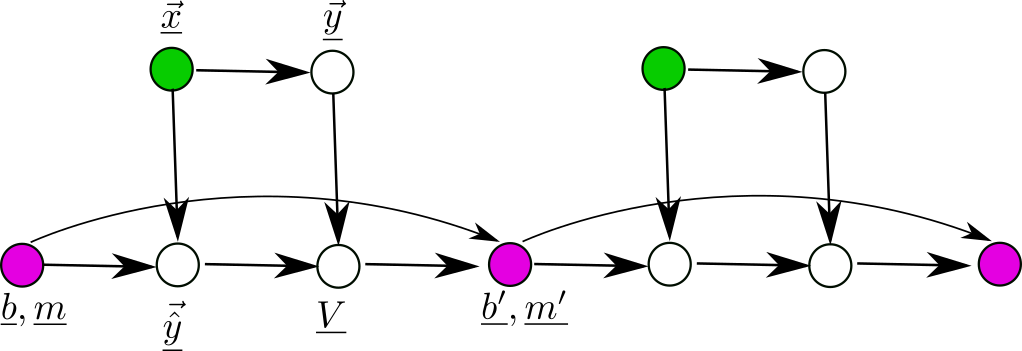
\includegraphics[width=5in]{linreg/linreg.png}
\caption{Linear Regression}
\label{fig-linreg}
\end{figure}

\begin{figure}[h!]
\centering
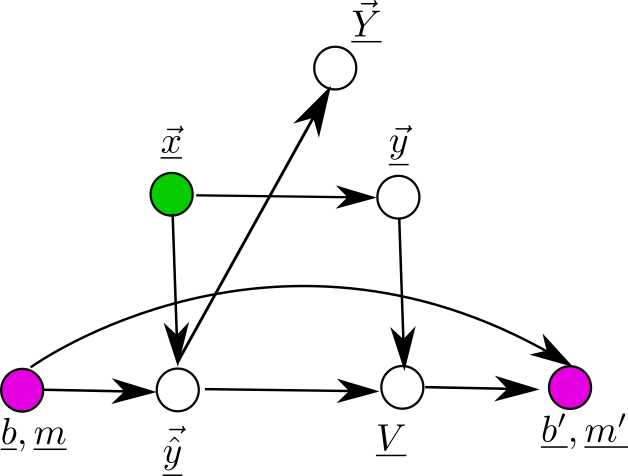
\includegraphics[width=3in]{linreg/linreg-emul.png}
\caption{Bnet of Fig.\ref{fig-linreg}  with new $\vec{\ul{Y}}$ node.}\label{fig-linreg-emul}
\end{figure}



Estimators $\haty$ for linear and logistic regression.
\begin{itemize}
\item

\textbf{Linear Regression:} $y\in \RR$.
Note $\haty\in \RR$. $(x,\haty(x))$ is
the graph
of a straight line
with y-intercept $b$ and slope $m$.
\beq
\haty(x;b, m)= b + mx
\eeq

\item
\textbf{Logistic Regression:} $y\in\{0, 1\}$. Note $\haty\in [0,1]$. $
(x,\haty(x))$ is the graph
of a sigmoid.
 Often in literature, $b,m$ are replaced by $\beta_0, \beta_1$.
\beq
\haty(x;b, m)=\smoid(b + m x)
\eeq
\end{itemize}

Define
\beq
V(b, m)=\sum_{x,y}P(x,y)| y-\haty(x;b, m)|^2
\;.\label{eq-norm-cost}
\eeq
We want to minimize $V(b,m)$ (called a cost or loss function) wrt $b$ and $m$.


The TPMs, printed in blue, for the
Bnet Fig.\ref{fig-linreg}, are as follows.

\beq\color{blue}
P(b,m) \text{ = given}
\eeq
The first time it is used,
$(b,m)$ is arbitrary.
After the first time, it is determined
by previous stage.

Let
\beq
P_{\rvx, \rvy}(x,y)=
\frac{1}{nsam(\vecx)}
\sum_\s \indi(x=x^\s, y=y^\s)
\;.
\eeq

\beq\color{blue}
P(\vecx)=\prod_\s P(x^\s)
\eeq

\beq\color{blue}
P(\vecy|\vecx)=\prod_\s P(y^\s\cond x^\s)
\eeq

\beq\color{blue}
P(\vec{\haty}|\vecx, b, m)=\prod_\s \delta(\haty^\s, \haty(x^\s,b,m))
\label{eq-replace1}
\eeq

\beq\color{blue}
P(V|\vec{\haty}, \vecy)=
\delta(V, \frac{1}{nsam(\vecx)}\sum_\s |y^\s-\haty^\s|^2)
\label{eq-replace2}
\eeq
Let $\eta_b, \eta_m>0$.
For $x=b,m$, if
$x'-x=\Delta x =
-\eta\frac{\partial V}{\partial x}$,
 then $\Delta V\approx
 \frac{-1}{\eta}(\Delta x)^2   \leq 0$
 for $\eta>0$. This is called \enquote{gradient descent}.
\beq\color{blue}
P(b'|V, b)=\delta(b', b-\eta_b\partial_b V)
\eeq
\beq\color{blue}
P(m'|V, m)=\delta(m', m-\eta_m\partial_m V)
\eeq


\section{Generalization to
$x$ with multiple
components (features)}

 Suppose that for each sample $\s$,
instead of $x^\s$ being a scalar,
it has $n$ components called features:

 \beq
x^\s = (x_0^\s, x_1^\s, x_2^\s , \ldots x_{n-1}^\s)
\;.\eeq

Slope $m$ is replaced by weights

\beq
w = (w_0, w_1, w_3, , \ldots, w_{n-1})
\;,\eeq
and the product of 2  scalars $mx^\s$ is replaced by the inner vector product $w^Tx^\s$.

\section{Alternative $V(b,m)$
 for logistic regression}

For logistic regression, since $y^\s\in \{0,1\}$
 and $\haty^\s\in [0,1]$ are both
in the interval $[0,1]$, they can
be interpreted as probabilities. Define
probability distributions $p^\s(x)$ and
$\HAT{p}^\s(x)$ for $x\in \{0,1\}$ by
\beq
p^\s(1)=y^\s,\;\;\; p^\s(0)=1-y^\s
\eeq

\beq
\HAT{p}^\s(1)=\haty^\s,\;\;\; \HAT{p}^\s(0)=1-\haty^\s
\eeq
Then for logistic regression, the following 2 cost functions $V(b,m)$
can be used as alternatives to the cost function Eq.(\ref{eq-norm-cost}) previously given.

\beq
V(b, m)= \frac{1}{nsam(\vecx)}\sum_\s
 D_{KL}(p^\s\parallel \HAT{p}^\s)
\eeq

and

\beqa
V(b, m)&=&\frac{1}{nsam(\vecx)} \sum_\s
CE(p^\s\parallel\HAT{p}^\s)\\
&=& \frac{-1}{nsam(\vecx)}\sum_\s \left\{
y^\s\ln \haty^\s +
(1-y^\s)\ln (1- \haty^\s)\right\}\\
&=&
\frac{-1}{nsam(\vecx)}\sum_\s
\ln \left\{(\haty^\s)^{y^\s}
(1- \haty^\s)^{(1-y^\s)}\right\}\\
&=&
\frac{-1}{nsam(\vecx)}\sum_\s
\ln P(\ul{Y}=y^\s\cond \haty=\haty^\s)\\
&=&
-\sum_{x,y} P(x, y)
\ln P(\ul{Y}=y|\haty=\haty(x,b,m))
\eeqa

Above, we used
\beq
P(\ul{Y}=Y|\haty) = \haty^{Y}
[1-\haty]^{1-Y}
\eeq
for $Y\in S_{\ul{Y}}=\{0,1\}$. (Bernoulli distribution).

There is no node corresponding to $\ul{Y}$
in the Bnet of Fig.\ref{fig-linreg}.
Fig.\ref{fig-linreg-emul} shows a new Bnet
that has a new node called $\vec{\ul{Y}}$
compared to the Bnet of Fig.\ref{fig-linreg}.
One defines the TPMs
for all nodes of Fig.\ref{fig-linreg-emul}
except $\vec{\ul{Y}}$ and $\ul{V}$ the same
as for Fig.\ref{fig-linreg}. For $\vec{\ul{Y}}$
and $\ul{V}$, one defines

\beq\color{blue}
P(Y^\s\cond \vec{\haty})=
P(\ul{Y}=Y^\s\cond \haty^\s)
\eeq

\beq\color{blue}
P(V|\vec{Y}, \vecy)=
\delta(V, \frac{-1}{nsam(\vec{x})}\ln  L)
\;,
\eeq
where $ L =\prod_\s P(\ul{Y}=y^\s\cond \haty^\s )$=likelihood.

\chapter{Linear Systems with Exogenous 
Noise}

In this chapter, we will consider 
bnets which were referred to,
prior to the invention of bnets, as:
Sewall Wright's Path Analysis (PA) and
linear Structural Equations Model (SEM).
Judea Pearl in his
books calls them
linear Structural Causal Models (SCM),
because they are very 
convenient for doing causal analysis.
We will follow 
Judea's convention
and refer to them as scum.


To 
build a SCM,
start with a deterministic bnet $G$.
Now  
add to each node $\rva$ of $G$ a 
root node $\rvU_\rva$
pointing into $\rva$ only.
The nodes $\rvU_\rva$ are called
the {\bf exogenous (external) variables}.
The exogenous
variables make their children noisy.
Their TPMs are
priors and are assumed 
to be unobserved.
Of course, by the
fact that they are 
root nodes, they are assumed 
to be mutually independent.

Examples:
\hrule


\begin{figure}[h!]
$$\xymatrix{
&\rvx\ar[dl]_\beta\ar[dr]^\alp
\\
\rvw\ar[dr]_\epsilon&&\rvz\ar[ll]_\gamma\ar[dl]^\delta
\\
&\rvy
}$$
\caption{}
\label{fig-scm-diamond}
\end{figure}

\beq\color{blue}
P(y|w, z, U_\rvy)=
\indi(y=\epsilon w +\delta z
+ U_\rvy)
\eeq

\beq\color{blue}
P(w|x, z, U_\rvw)=
\indi(w=\beta x +\gamma z + U_\rvw)
\eeq

\beq\color{blue}
P(z|x, U_\rvz)=
\indi(z=\alpha x + U_\rvz)
\eeq

\beq\color{blue}
P(x|U_\rvx)=
\indi(x=U_\rvx)
\eeq

\beqa
y&=&
\epsilon w +\delta z
+ U_\rvy
\\
&=&
\epsilon (\beta x +\gamma z + U_\rvw)
 +\delta z
+ U_\rvy
\\
&=&
(\epsilon\gamma + \delta)z
+ \epsilon\beta x
+\epsilon U_\rvw U_\rvy
\\
&=&
(\epsilon\gamma + \delta)z
+ \epsilon\beta U_\rvx
+\epsilon U_\rvw U_\rvy
\eeqa

\beq
\left(\pder{y}{z}\right)_{U.}=
\epsilon\gamma + \delta
\eeq
sum of terms,
each of those terms
represents a different
causal (not blocked)
path from $\rvz$ to $\rvy(\rvz)$.


\hrule
bnet
with 
deterministic nodes
$\rvx.=(\rvx_k)_{k=0, 1, \ldots nx-1}$
and 
corresponding exogenous nodes 
$\rvU.=(\rvU_k)_{k=0, 1, \ldots nx-1}$.
Assume $\av{\rvU_i, \rvU_j}=0$
if $i\neq j$. The {\bf structural
coefficient} $\alp_{j|i}> 0$
measures the strength of
the connection 
$\rvx_i\rarrow \rvx_j$.
$\av{\rvx, \rvy}$ notation,
for 
covariances 
of any two random variables $\rvx, \rvy$
is explained in the 
Notational
Conventions chapter \ref{ch-not-cons}.

\begin{itemize}

\item {\bf Fully connected graph with $nx=2$}

\begin{figure}[h!]
$$
\xymatrix{
\rvx_0
\ar[d]^{\alp{1|0}}
\\
\rvx_1
}$$
\caption{
Fully connected graph with 2 $\rvx_j$
(exogenous nodes $\rvU_j$
not shown).}
\label{fig-fully-conn-2}
\end{figure}

\begin{subequations}
\label{eq-fully-conn-2}
\beqa
\rvx_0&=&\rvU_0
\\
\rvx_1&=&\alp_{1|0}\rvx_0  + \rvU_1
\eeqa
\end{subequations}
Eqs.\ref{eq-fully-conn-2}
constitute a system of 2 
linear equations in 2 unknowns
(the $\rvx$'s) so can solve
for the $\rvx$'s in terms 
of the $\alpha$'s and $\rvU$'s.


\beq
\av{\rvx_1, \rvx_0}=
\alp_{1|0}\av{\rvx_0, \rvx_0}
\eeq
Thus, $\alp_{1|0}$
can be estimated  
from the covariances $\av{\rvx_i, \rvx_j}$.

\item {\bf Fully connected graph with $nx=3$}

\begin{figure}[h!]
$$
\xymatrix{
\rvx_0\ar[d]_{\alp_{1|0}}
\ar[dr]^{\alp_{2|0}}
\\
\rvx_1\ar[r]^{\alp_{2|1}}
&\rvx_2
}$$
\caption{
Fully connected graph with 3 $\rvx_j$
(exogenous nodes $\rvU_j$
not shown).}
\label{fig-fully-conn-3}
\end{figure}


\begin{subequations}
\label{eq-fully-conn-3}
\beqa
\rvx_0 &=& \rvU_0
\\
\rvx_1&=&\alp_{1|0}\rvx_0 + \rvU_1
\\
\rvx_2&=&\alp_{2|1}\rvx_1 +
\alp_{2|0}\rvx_0 +\rvU_2
\eeqa
\end{subequations}
Eqs.\ref{eq-fully-conn-3}
constitute a system of
3 linear  equations in 3 unknowns
(the $\rvx$'s) so can solve
for the $\rvx$'s in terms 
of the $\alpha$'s and $\rvU$'s.


\begin{subequations}
\label{eq-fully-conn-3-covs}
\beqa
\av{\rvx_1, \rvx_0}&=&
\alp_{1|0}\av{\rvx_0, \rvx_0}
\\
\av{\rvx_2, \rvx_0}&=&
\alp_{2|1}\av{\rvx_1, \rvx_0}
+
\alp_{2|0}\av{\rvx_0, \rvx_0}
\\
\av{\rvx_2, \rvx_1}&=&
\alp_{2|1}\av{\rvx_1, \rvx_1}
+
\alp_{2|0}\av{\rvx_0, \rvx_1}
\eeqa
\end{subequations}
Eqs.\ref{eq-fully-conn-3-covs}
constitute a system of
3 linear  equations in 3 unknowns
(the $\alpha$'s) so can solve
solve for the $\alpha$'s in terms
of covariances $\av{\rvx_i, \rvx_j}$.
This gives an estimate
for the $\alp$'s. 

\end{itemize}
\chapter{Markov Blankets}\label{ch-mblanket}


This chapter is based on the
Wikipedia article, 
Ref.\cite{wiki-mblanket}.
Markov blankets
and Markov boundaries of bnets
were apparently invented
by Judea Pearl. His 1988 book
 Ref.\cite{pearl-1988book},
instead of a research paper, is 
usually given as the original reference.

\begin{figure}[h!]
\centering
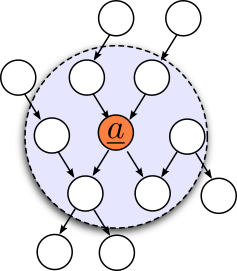
\includegraphics[width=1.5in]{mblanket/mblanket.png}
\caption{In a bnet,
the minimal Markov blanket,
aka Markov boundary,
of node $\rva$.} 
\label{fig-mblanket}
\end{figure}

We will treat vectors 
of random variables as if
they were sets when using the $\in$,
$\subset$ and $-$ operations.
For example,
if $\rvx=(\rvx_0, 
\rvx_1, \rvx_2,
\rvx_3)$ and
$\rvb=(\rvx_1, \rvx_2)$,
then $\rvx_1\in \rvb\subset \rvx$ and
$\rvx-\rvb=(\rvx_0, \rvx_3)$.

Below, $H(\rva:\rvb|\rvc)$
denotes the conditional
mutual information of
random variables
$\rva$ and $\rvb$
conditioned on 
random variable $\rvc$.
$H(\rva:\rvb|\rvc)$
is used in Shannon Information
Theory, where it is defined by

\beq
H(\rva:\rvb|\rvc)=
\sum_{a,b,c}
P(a,b,c)\ln 
\frac{P(a,b|c)}{P(a|c)P(b|c)}
\;.
\eeq
$H(\rva:\rvb|\rvc)=0$
iff $\rva$ and $\rvb$
are independent (uncorrelated)
when $\rvc$ is held fixed.



Suppose
$\rva\in  \rvX$,
 $\rvB\subset \rvX$,
but $\rva\notin\rvB$.
Then $\rvB$ is a Markov blanket
of $\rva$ if

\beq
H(\rva: \rvX-\rva|\rvB)=0
\;.
\eeq
In other words, one may assume that
$\rva$ depends on $\rvB$ only, 
and is independent of all random
variables in $\rvX-(\rva\cup\rvB)$.

The minimal Markov blanket 
is called the Markov boundary.

In a bnet, the Markov boundary
of a node $\rva$,
contains:
\begin{enumerate}
\item
the parents of $\rva$,
\item
the children of $\rva$,
\item
the parents, other than $\rva$,
of the children of $\rva$.
\end{enumerate}
This is illustrated in 
Fig.\ref{fig-mblanket}.
\chapter{Markov Chains}

A Markov Chain is simply
a bnet with the graph structure 
of a chain. For example,
Fig.\ref{fig-mchain}
shows a chain with $n=4$ nodes.

\begin{figure}[h!]
\centering
$$\xymatrix{
\rvx_0\ar[r]
&\rvx_1\ar[r]
&\rvx_2\ar[r]
&\rvx_3
}$$
\caption{Markov chain with $n=4$ nodes.}
\label{fig-mchain}
\end{figure}

Because of its
 graph structure,
the TPM of each node
only depends on the state of the previous 
node:

\beq
P(x_t|(x_a)_{a\neq t})=P(x_t|x_{t-1})
\;,
\eeq
where $(x_a)_{a\neq t}$ are all
 the nodes except $x_t$ itself and
$t=1, 2, \dots, n-1$.

If there
exists a single
TPM $P_{\rvx_1|\rvx_0}$
such that

\beq
P(x_t|x_{t-1})=P_{\rvx_1|\rvx_0}
(x_t|x_{t-1})
\;
\eeq
for $t=1, 2,\dots, n-1$, 
then
we say 
that the Markov chain
is {\bf time homogeneous}.
\chapter{Markov Chain Monte Carlo (MCMC)}


Monte Carlo methods
are methods for using
 random number generation to
sample probability distributions.
The subject of Monte Carlo methods
has many branches, as you can see 
from its Wikipedia
category list, Ref.\cite{wiki-monte-carlo}.
MCMC (Markov
Chain Monte Carlo) is just one of those
branches, albeit a major one.
Metropolis-Hastings (MH) sampling
is a very important MCMC method.
Gibbs sampling is
a special case
of MH sampling.
This chapter covers both, MH and Gibbs sampling.
It also covers a few 
other types of sampling.


\section*{Inverse Cumulative Sampling}
For more info about this topic 
and some original references, 
see Ref.\cite{wiki-inv-cum}.

This
is one of the simplest
methods for obtaining
samples from a probability 
distribution $P_\rvx$,
but it
requires knowledge
of the inverse
 cumulative distribution
of $P_\rvx$, which
is often not available.

The {\bf cumulative
distribution} function
is defined by:

\beq
CUM_\rvx(x)=P(\rvx<x)=
\int_{x'<x} dx'\;P_\rvx(x')
\;.
\eeq
Note that

\beq
P_\rvx(x)=\frac{d}{dx}CUM_\rvx(x)
\;.
\eeq


\begin{figure}[h!]
$$\xymatrix{
\rvu^{(0)}\ar[d]
&\rvu^{(1)}\ar[d]
&\rvu^{(2)}\ar[d]
\\
\ul{\vecx}^{(0)}\ar[r]
&\ul{\vecx}^{(1)}\ar[r]
&\ul{\vecx}^{(2)}
}$$
\caption{bnet for Inverse Cumulative Sampling}
\label{fig-mcmc-inverse-bnet}
\end{figure}

For $t=0, 1, \ldots, T-1$, let

$\rvu^{(t)}\in [0,1]$= random variable, 
uniformly
distributed over $[0,1]$.

$\ul{\vecx}^{(t)}=[\rvx^{(t)}_i]_{i=0,1, nsam(t)-1}$
where $\rvx^{(t)}_i \in S_\rvx$ for all $i$. 
Vector of samples collected 
up to time $t$.

The transition prob matrices, printed
in blue, for  the nodes of bnet
 Fig.\ref{fig-mcmc-inverse-bnet}, are:

\beq\color{blue}
P(u^{(t)})=1
\eeq

\beq\color{blue}
P(\vecx^{(t)}|\vecx^{(t-1)}, u^{(t)})=
\indi(\;\;\;\vecx^{(t)}=
[\vecx^{(t-1)}, CUM^{-1}_\rvx(u^{(t)})]
\;\;\;)
\eeq

\hrule\noindent
{\bf Motivation}

\begin{figure}[h!]
\centering
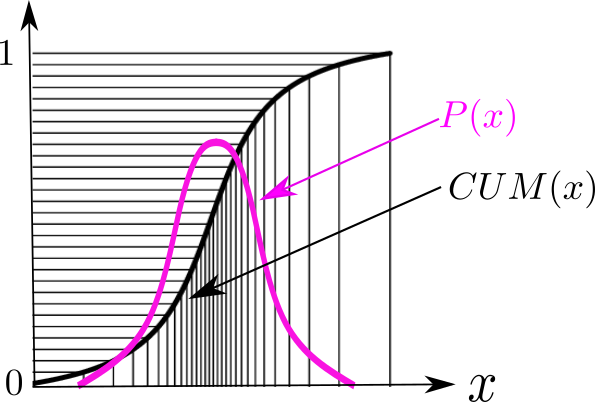
\includegraphics[width=3in]
{mcmc/inverse.png}
\caption{Motivation 
for Inverse of Cumulative Sampling.} 
\label{fig-mcmc-inverse}
\end{figure}
See Fig.\ref{fig-mcmc-inverse}.


Note that if 
$\rvu$ is uniformly distributed over 
the interval $[0,1]$ and $a\in[0,1]$, then

\beq
P(\rvu<a)=a
\;.
\eeq
Thus

\beqa
P(CUM^{-1}_\rvx(\rvu)<x)
&=&P(\rvu<CUM_\rvx(x))
\\
&=&CUM_\rvx(x)
\;.
\eeqa
Therefore,

\beq
P_\rvx(x)dx=dP(CUM^{-1}_\rvx(\rvu)<x)
\;.
\eeq


\section*{Rejection Sampling}

For more info about this topic 
and some original references, 
see Ref.\cite{wiki-reject}.


\begin{figure}[h!]
$$\xymatrix{
&\rvu^{(0)}\ar[d]
&&\rvu^{(1)}\ar[d]
&&\rvu^{(2)}\ar[d]
\\
\ul{\vecx}^{(0)}\ar@/^1pc/[rr]
&\rva^{(0)}\ar[r]
&
\ul{\vecx}^{(1)}\ar@/^1pc/[rr]
&\rva^{(1)}\ar[r]
&
\ul{\vecx}^{(2)}\ar@/^1pc/[rr]
&\rva^{(2)}\ar[r]
&\ul{\vecx}^{(3)}
\\
&\rvc^{(0)}\ar[u]\ar[ru]
&&\rvc^{(1)}\ar[u]\ar[ru]
&&\rvc^{(2)}\ar[u]\ar[ru]
}$$
\caption{bnet for Rejection Sampling}
\label{fig-mcmc-reject-bnet}
\end{figure}

For $t=0, 1, \ldots, T-1$, let

$\rvu^{(t)}\in [0,1]$= random variable, 
uniformly
distributed over $[0,1]$.

$\rva^{(t)}\in \bool$= accept candidate? (no=0, yes=1)

$\rvc^{(t)}\in S_\rvx$=  sample that is a 
candidate for being accepted

$\ul{\vecx}^{(t)}=
[\rvx^{(t)}_i]_{i=0,1, nsam(t)-1}$
where $\rvx^{(t)}_i \in S_\rvx$ for all $i$. 
Vector of samples collected 
up to time $t$.

Assume that
\beq
P_\rvx(x)< \beta P_\rvx(x)
\eeq
for all $x\in S_\rvx$ and some $\beta\in \RR$.

The transition prob matrices, printed
in blue, for  the nodes of bnet
 Fig.\ref{fig-mcmc-reject-bnet}, are:


\beq\color{blue}
P(u^{(t)}=u)=1
\eeq

\beq\color{blue}
P(\rvc^{(t)}=c)=P_\rvx(c)
\eeq

\beq\color{blue}
P(\rva^{(t)}=a|\rvc^{(t)}=c,
\rvu^{(t)}=u)=
\left\{
\begin{array}{ll}
\delta(a, 0)&\text{ if }
u \beta P_\rvx(c)\geq P_\rvx(c))
\\
\delta(a, 1)&\text{ if }
u \beta P_\rvx(c)< P_\rvx(c))
\end{array}
\right.
\eeq

\beq\color{blue}
P(\vecx^{(t)}|
\vecx^{(t-1)}, \rva^{(t)}=a, \rvc^{(t)}=c)
=
\left\{
\begin{array}{ll}
\delta(\vecx^{(t)}, \vecx^{(t-1)})
& \text{ if $a=0$}
\\
\delta(\vecx^{(t)}, [\vecx^{(t-1)}, c])
&\text{ if $a=1$}
\end{array}
\right.
\eeq

\hrule\noindent
{\bf Motivation}

\begin{figure}[h!]
\centering
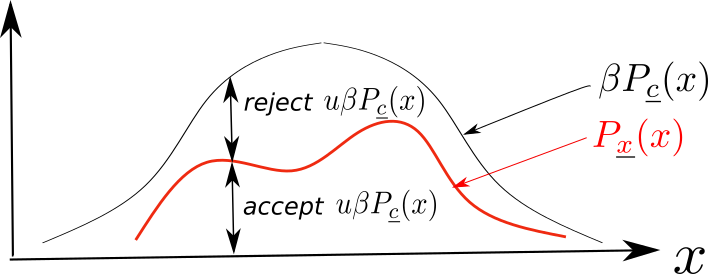
\includegraphics[width=3.5in]
{mcmc/reject.png}
\caption{Motivation 
for Rejection Sampling.} 
\label{fig-mcmc-reject}
\end{figure}
See Fig.\ref{fig-mcmc-reject}.

\section*{Metropolis-Hastings Sampling}

For more info about this topic and 
some original references, 
see Refs.\cite{bendel-metro-hast}
and \cite{wiki-metro-hast}.

A very convenient
feature of this method is that it can sample
unnormalized probability distributions
$(constant)P_\rvx$ 
because it 
only uses ratios of
$P_\rvx$ at two different points.



\begin{figure}[h!]
$$\xymatrix{
&\rvu^{(0)}\ar[d]
&&\rvu^{(1)}\ar[d]
&&\rvu^{(2)}\ar[d]
\\
\ul{\vecx}^{(0)}\ar@/^1pc/[rr]
&\rva^{(0)}\ar[r]
&
\ul{\vecx}^{(1)}\ar@/^1pc/[rr]\ar[rdd]
&\rva^{(1)}\ar[r]
&
\ul{\vecx}^{(2)}\ar@/^1pc/[rr]\ar[rdd]
&\rva^{(2)}\ar[r]
&\ul{\vecx}^{(3)}
\\
&\rvc^{(0)}\ar[u]\ar[ru]
&&\rvc^{(1)}\ar[u]\ar[ru]
&&\rvc^{(2)}\ar[u]\ar[ru]
\\
&\rvm^{(0)}\ar[u]\ar@/^1pc/[uu]
&&\rvm^{(1)}\ar[u]\ar@/^1pc/[uu]
&&\rvm^{(2)}\ar[u]\ar@/^1pc/[uu]
}$$
\caption{bnet for Metropolis-Hastings Sampling}
\label{fig-mcmc-metro-bnet}
\end{figure}

For $t=0, 1, \dots, T-1$, let

$\rvu^{(t)}\in [0,1]$= random variable,
uniformly
distributed over $[0,1]$.

$\rva^{(t)}\in \bool$= accept candidate? (no=0, yes=1)

$\rvc^{(t)}\in S_\rvx$= sample that is a 
candidate for being accepted

$\rvm^{(t)}\in S_\rvx$= memory
of last accepted sample

$\ul{\vecx}^{(t)}=[\rvx^{(t)}_i]_{i=0,1, nsam(t)-1}$
where $\rvx^{(t)}_i \in S_\rvx$ for all $i$. 
Vector of samples collected 
up to time $t$.

A {\bf proposal transition prob matrix} 
$P_{\rvc|\rvx}:S_\rvx^2\rarrow [0,1]$ 
must be specified a priori 
for this algorithm.

The transition prob matrices, printed
in blue, for  the nodes of bnet
 Fig.\ref{fig-mcmc-metro-bnet}, are:

\beq\color{blue}
P(u^{(t)}=u)=1
\eeq

\beq\color{blue}
P(\rvc^{(t)}=c|m^{(t)}=m)=P_{\rvc|\rvx}(c|m)
\eeq

\beq\color{blue}
P(\rva^{(t)}=a|\rvc^{(t)}=c,
\rvu^{(t)}=u,m^{(t)}=m)=
\left\{
\begin{array}{ll}
\delta(a, 0)&\text{ if }
u \geq \alp(c|m)
\\
\delta(a, 1)&\text{ if }
u < \alp(c|m)
\end{array}
\right.
\eeq
where the 
{\bf acceptance probability}
 $\alp$ is defined as

\beq
\alp(c|m)=\min\left(1,
\frac
{P_{\rvc|\rvx}(m|c)P_\rvx(c)} 
{P_{\rvc|\rvx}(c|m)P_\rvx(m)}
\right)
\;.
\eeq
Note that if the proposal distribution
is symmetric, then

\beq
\alp(c|m)=\min\left(1,
\frac
{P_\rvx(c)} 
{P_\rvx(m)}
\right)
\;.
\eeq

\beq\color{blue}
P(\vecx^{(t)}|
\vecx^{(t-1)}, \rva^{(t)}=a, \rvc^{(t)}=c)
=
\left\{
\begin{array}{ll}
\delta(\vecx^{(t)}, \vecx^{(t-1)})
& \text{ if $a=0$}
\\
\delta(\vecx^{(t)}, [\vecx^{(t-1)}, c])
&\text{ if $a=1$}
\end{array}
\right.
\eeq

\beq\color{blue}
P(\rvm^{(t)}=m|
\vecx^{(t)})=
\delta(m, \text{last component of }
\vecx^{(t)}
)
\eeq

\hrule\noindent
{\bf Motivation}

\begin{figure}[h!]
\centering
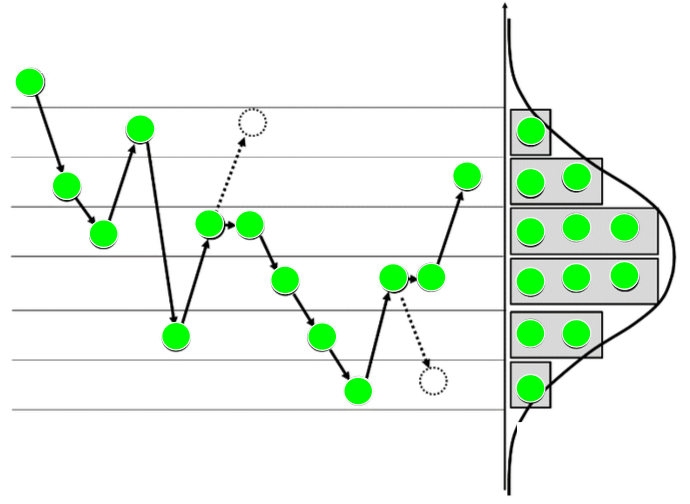
\includegraphics[width=3.5in]
{mcmc/metro-hast.png}
\caption{Motivation 
for Metropolis-Hastings Sampling.} 
\label{fig-metro-hast}
\end{figure}
See Fig.\ref{fig-metro-hast}.


Consider a time homogeneous (its
transition
matrix is the same for all times)
Markov chain with
transition prob $P(x'|x)=[T]_{x', x}$.
It's {\bf stationary distribution}, 
if it exists, is
defined as 

\beq 
\pi=\lim_{n\rarrow\infty}T^n\pi_0
\;.
\eeq

Suppose the prob distribution $P_\rvx(x)$
that we wish to sample from
satisfies

\beq
P_\rvx(x)=\pi(x)
\;.
\eeq

{\bf Reversibility (detailed balance):}
\beq
P(x'|x)\pi(x)=P(x|x')\pi(x')
\;.
\eeq
Detailed balance
is a sufficient (although not
necessary) condition
for the stationary 
distribution $\pi$ to exist.

Let
\beq
P(x'|x)=
P(a=1|x',x)P_{\rvc|\rvx}(x'|x)
+\delta(x,x')P(a=0|x)
\;,
\eeq
where

\beq
P(a=0|x)=\sum_{x'} P(a=0|x',x)P_{\rvc|\rvx}(x'|x)
\;.
\eeq

\begin{claim}
If

\beq
P(a=1|x',x)=\alpha(x'|x)
\;,
\eeq
then detailed balance is satisfied.
\end{claim}
\proof
Assume $x\neq x'$.

\beqa
P(x'|x)P(x)&=&
P(a=1|x',x)P_{\rvc|\rvx}(x'|x)P_\rvx(x)
\\
&=&
\min\left(1,
\frac
{P_{\rvc|\rvx}(x|x')P_\rvx(x')} 
{P_{\rvc|\rvx}(x'|x)P_\rvx(x)}
\right)
P_{\rvc|\rvx}(x'|x)P_\rvx(x)
\\
&=&
\min\left(P_{\rvc|\rvx}(x'|x)P_\rvx(x),
{P_{\rvc|\rvx}(x|x')P_\rvx(x')} 
\right)
\\
&=&
P(x|x')P(x')
\eeqa
\qed


\section*{Gibbs Sampling}
For more info about this topic and some 
original references, 
see Ref.\cite{wiki-gibbs-sam}.

Gibbs sampling is a special case
of Metropolis-Hastings sampling.
Gibbs
 sampling is ideally 
suited for application
to a bnet, because
it is stated in
terms of the conditional 
prob distributions
of $N$ random variables,
and conditional 
prob distributions are part of
the definition of a bnet.

Consider a bnet with
nodes $\rvx_0, \rvx_1, \ldots, \rvx_{N-1}$

Identify
the random
variable  $\rvx=(\rvx_0, \rvx_1, \ldots, \rvx_{N-1})$
with the
random variable  $\rvx$ used in 
Metropolis-Hastings sampling.
For Gibbs sampling,
we use the following proposal function:

\beq
P_{\rvc|\rvx}(c|m)=
\prod_{j=0}^{N-1}
P(c_j\cond [m_i]_{i\neq j})
\;.
\label{eq-gibbs-proposal}
\eeq
Eq.(\ref{eq-gibbs-proposal})
can be simplified using 
Markov Blankets
 (see Chapter \ref{ch-mblanket})
to the following:

\beq
P_{\rvc|\rvx}(c|m)=
\prod_{j=0}^{N-1}
P(c_j\cond[m_i: \forall i \ni\rvm_i\in MB(\rvc_j)])
\;,
\eeq
where for any node $\rva$,
we denote its Markov blanket by $MB(\rva)$.


\section*{Importance Sampling}

For more info about this topic and some 
original references, 
see Ref.\cite{wiki-imp-sam}.

Suppose random
variables $\rvx[s]$ for
$s=0, 1, \ldots nsam-1$ are i.i.d.
with probability distribution$P_\rvx$. Then
\beq
E_{\rvx}[f(x)]\approx 
\frac{1}{nsam}\sum_{s=0}^{nsam-1}
f(x[s])
\;.
\eeq
Sometimes,
instead of using i.i.d.
samples $x[s]\sim P_\rvx$,
we wish to use i.i.d. samples
$y[s]\sim P_\rvy$,
where both $\rvx[s]\in S_\rvx$
and $\rvy[s]\in S_\rvx$.


\beqa
E_\rvx[f(\rvx)]
&=&
\sum_x P_\rvx(x)f(x)
\\&=&
\sum_x P_\rvy(x))\frac{P_\rvx(x)}{P_\rvy(x)}f(x
\\&=&
E_{\rvy}[
\frac{P_\rvx(y)}{P_\rvy(y)}f(y)
]
\eeqa

Sampling from $P_\rvy(y)$ instead
of $P_\rvx(x)$
might reduce (or increase) 
variance for a particular
 $f:S_\rvx\rarrow \RR$.

\beq
Var_\rvx[f(x)]=
E_\rvx[(f(x))^2]-(E_\rvx[f(x)])^2
\eeq

\beqa
Var_\rvy[\frac{P_\rvx(y)}{P_\rvy(y)}f(y)]&=&
E_\rvy[(\frac{P_\rvx(y)}{P_\rvy(y)}f(y))^2]-
(E_\rvy[\frac{P_\rvx(y)}{P_\rvy(y)}f(y)])^2
\\
&=&
E_\rvx[\frac{P_\rvx(x)}{P_\rvy(x)}(f(x))^2]-
(E_\rvx[f(x)])^2
\eeqa





\chapter{Missing Data, Imputation}
\label{ch-missing-d}

This chapter assumes
that the reader has
read some parts of
Chapter \ref{ch-emax}
on the Expectation
Maximization
(EM) algo
and Chapter \ref{ch-mcmc}
on Markov Chain Monte Carlo
(MCMC).


\begin{table}[h!]
\centering
\begin{tabular}{|
>{\columncolor[HTML]{ECF4FF}}l |l|l|l|l|}
\hline
 & \cellcolor[HTML]{ECF4FF}$h_0$ & \cellcolor[HTML]{ECF4FF}$x_0$ & \cellcolor[HTML]{ECF4FF}$x_1$ & \cellcolor[HTML]{ECF4FF}$x_2$ \\ \hline
1 & NA & 0 & 1 & 1 \\ \hline
2 & NA & 0 & 0 & 0 \\ \hline
3 & NA & 1 & 1 & 0 \\ \hline
4 & NA & NA & 1 & NA \\ \hline
5 & NA & 0 & NA & 1 \\ \hline
6 & NA & 0 & 0 & 1 \\ \hline
\end{tabular}
\;\;\;\;
\begin{tabular}{|
>{\columncolor[HTML]{ECF4FF}}l |l|l|l|l|l|}
\hline
 & \cellcolor[HTML]{ECF4FF}$h_0$ & \cellcolor[HTML]{ECF4FF}$x_0$
 & \cellcolor[HTML]{ECF4FF}$x_1$ & \cellcolor[HTML]{ECF4FF}$x_2$ 
& \cellcolor[HTML]{DAE8FC}$m$ \\ \hline
1 & NA & 0 & 1 & 1 & (0,0,0) \\ \hline
2 & NA & 0 & 0 & 0 & (0,0,0) \\ \hline
3 & NA & 1 & 1 & 0 & (0,0,0) \\ \hline
4 & NA & \begin{tabular}[c]{@{}l@{}}0\\ 0\\ 1\\ 1\end{tabular} & 1 & \begin{tabular}[c]{@{}l@{}}0\\ 1\\ 0\\ 1\end{tabular} & (1,0,1) \\ \hline
5 & NA & 0 & \begin{tabular}[c]{@{}l@{}}0\\ 1\end{tabular} & 1 & (0,1,0) \\ \hline
6 & NA & 0 & 0 & 1 & (0,0,0) \\ \hline
\end{tabular}
\caption{{\bf Left Table:}
Dataset 
with 
$nsam=6$ and some missing entries,
 for 4 binary variables $h_0, x_0, x_1, x_2$.
 NA=not available.
The $h_0$  column is completely missing 
because $h_0$ is an unobserved latent 
variable.
{\bf Right Table:} All possibilities
for
$x_i=NA$ cells of left table have
been enumerated. A new column
labeled $m$ has been added.
$m_i=\indi(x_i \text{ is missing})$
for $i=0,1,2$.}
\label{tab-missing-data}
\end{table}


Suppose that you
have compiled a {\bf dataset}
$\vec{x}=(x[\sigma])_{\sigma=0, 1, \ldots,
nsam-1}$
where $x=(x_0, x_1, \ldots,x_{ nx-1})$
from a study or survey.
It consists 
of $nsam$ number 
of samples (sample= row), 
and $nx$ columns (each column is a different 
feature, or observation).
Suppose that some of the
cells
in this matrix 
are empty.
Throwing
away all the incomplete
rows is okay 
if the 
number
of incomplete rows
is much smaller  than
$nsam$.
If not,
throwing 
them
away would
throw away
a substantial amount of
information 
contained in all the
filled cells
in those incomplete rows, 
plus it might
bias your dataset.
This chapter
deals with
how to fill
those empty cells 
with plausible
fake data.
A fancy name
for this process
is {\bf imputation}.
There is no unique
way of 
fabricating
fake data,
but
some fakes
are
better than others
by some metrics.
This chapter will
consider
two popular
ways (EM
and MCMC)
of 
filling those
empty 
cells
with
their
``most likely" values
based on the cells
of the dataset that
aren't missing,
and
also based
on some bnet
model
that is 
expected to describe well the
dataset.

Notation:
$\vec{\rva}=
(\rva[\sigma])_{\sigma=0, 1, \ldots,nsam-1}
$, where $nsam$
is the number of samples.
Will
sometimes
denote
$a\sqsig$ by $a^\sqsig$.


For concreteness,
we will
apply
the concepts
of this chapter
to
the dataset
with missing data
given by Table \ref{tab-missing-data}.


\section*{Imputation via EM}

We begin by augmenting
Fig.\ref{fig-em-bnet} (the first figure
in Chapter \ref{ch-emax})
by adding to it a new node
$\vec{\rvm}$
called the
{\bf missingness variable}.
Recall
that node
$\ul{\theta}$
represents
the {\bf unknown parameters},
node $\vec{\rvx}$
represents the
{\bf observed variables},
and 
node $\vec{\rvh}$
represents the {\bf latent
variables}.
Both $\ul{\theta}$
and $\vec{\rvh}$
are hidden (i.e., unobserved).
Fig.\ref{fig-mar}
shows
3
popular
ways of 
connecting node $\vec{\rvm}$
 to the
other nodes
in the graph Fig.\ref{fig-em-bnet}.



\begin{figure}[h!]
$$
\begin{array}{ccc}
\xymatrix{
&\ul{\theta}\ar[d]\ar[ld]\ar[rd]
\\
\vec{\rvm}
&\vec{\rvx}
&\vec{\rvh}\ar[l]
}
&
\xymatrix{
&\ul{\theta}\ar[d]\ar[ld]\ar[rd]
\\
\vec{\rvm}
&\vec{\rvx}\ar[l]
&\vec{\rvh}\ar[l]
}
&
\xymatrix{
&\ul{\theta}\ar[d]\ar[ld]\ar[rd]
\\
\vec{\rvm}
&\vec{\rvx}\ar[l]
&\vec{\rvh}\ar[l]\ar@/^1pc/[ll]
}
\\
\\
\text{Seldom assumed}
&\text{MAR}
&\text{not-MAR (NMAR)}
\end{array}
$$
\caption{The 
left bnet is seldom assumed. The
middle bnet 
is referred to as the MAR (missing
at random)
assumption. The right bnet
is referred to as the not-MAR  (NMAR)
assumption.}
\label{fig-mar}
\end{figure}



From Fig.\ref{fig-mar}, we have
\beq
P(\vec{m}|\vec{x},
\vec{h}, \theta)=
\left\{
\begin{array}{ll}
P(\vec{m}| \theta)&\text{Seldom assumed. Called missing-CAR (MCAR)}
\\
P(\vec{m}|\vec{x}, \theta)&\text{MAR}
\\
P(\vec{m}|\vec{x}, \vec{h}, \theta)
&\text{not-MAR (NMAR)}
\end{array}
\right.
\;.
\eeq

For
doing imputation
via EM, 
we connect node
$\vec{\rvm}$
as shown in the
middle bnet (called MAR)
of Fig.\ref{fig-mar}.


\begin{figure}[h!]
$$
\begin{array}{ccc}
\xymatrix{
&\ul{\theta}\ar[d]\ar[dr]\ar[dl]
\\
\vec{\rvm}
&\ul{\vecx}\ar[l]
&\ul{\vech}\ar[l]
}
&=&
\xymatrix{
&\ul{\theta}\ar[ld]\ar[ldd]\ar[lddd]
\ar[d]
\ar@/_1pc/[dd]
\ar@/_1pc/[ddd]
\ar[rd]\ar[rdd]\ar[rddd]
\\
\rvm[0]
&
\rvx[0]\ar[l]
&\rvh[0]\ar[l]
\\
\rvm[1]
&
\rvx[1]\ar[l]
&\rvh[1]\ar[l]
\\
\rvm[2]
&
\rvx[2]\ar[l]
&\rvh[2]\ar[l]
}
\end{array}
$$
\caption{MAR bnet
with $nsam=3$.}
\label{fig-mar-multi}
\end{figure}

For the example of
Table \ref{tab-missing-data},
we have
variables
$\vec{\rvm},\vec{\rvx}$
and $\vec{\rvh}$
whose values range over the 
following sets:

$\vec{\rvx}=(\vec{\rvx}_0, \vec{\rvx}_1, 
\vec{\rvx}_2)$

$\vec{\rvh}=(\vec{\rvh}_0)$

$\rvh_0[\sigma]\in\bool$,

$\rvx_i[\sigma]\in\bool$
for $i=0,1,2$,

$\rvm_i[\sigma]\in\bool$
for $i=0,1,2$.



\begin{figure}[h!]
$$\xymatrix{
\rvm[0]
&\rvx[0]\ar[l]
&\rvh[0]\ar[l]
}=
\;\;\;\;\;
\xymatrix{
\rvm[0]
&\rvx_0[0]\ar[l]\ar[d]\ar@/^1pc/[dd]
&\rvh[0]\ar[ld]
\ar@{-->}[ldd]
\ar@{-->}[l]
\\
&\rvx_1[0]\ar[ul]\ar[d]
\\
&\rvx_2[0]\ar[uul]
}
$$
\caption{Our example for imputation via
 EM
assumes this bnet
between nodes
$\rvm[\sigma],
\rvx[\sigma], \rvh[\sigma]$.}
\label{fig-miss-subnet}
\end{figure}

For
concreteness,
we will assume
that 
the Markov
chain
$\rvm[\sigma]\larrow
\rvx[\sigma]\larrow\rvh[\sigma]$
has a finer grained DAG structure
given by Fig.\ref{fig-miss-subnet}.
where we will
omit the dashed arrows.
If one
doesn't
want
to assume that the data
can be fitted
well by the
bnet
of 
Fig.\ref{fig-miss-subnet}
without
the dashed arrows,
one can include those arrows too,
at the expense of more 
unknown parameters
(i.e., degrees of freedom)
to be lumped into $\theta$.
We will parmaterize
the TPMs 
corresponding
to Fig.\ref{fig-miss-subnet}
using a 
Categorical Distribution
for each column of the
TPMs.
We will thus assume
that the bnet of 
Fig.\ref{fig-miss-subnet}
has the following TPMs,
printed in blue.

\beq\color{blue}
P(h_0^\sqsig| \theta)=
\begin{array}{l|l}
\\\hline
&1-\theta_0
\\
{\scriptstyle 1}&\theta_0
\end{array}
\eeq

\beq\color{blue}
P(x_0^\sqsig| \theta)=
\begin{array}{l|l}
\\\hline
{\scriptstyle 0}&1-\theta_1
\\
{\scriptstyle 1}&\theta_1
\end{array}
\eeq


\beq\color{blue}
P(x_1^\sqsig\cond x_0^\sqsig, h^\sqsig, \theta)=
\begin{array}{l|llll}
&{\scriptstyle 00}
&{\scriptstyle 01}
&{\scriptstyle 10}
&{\scriptstyle 11}
\\\hline
{\scriptstyle 0}
&1-\theta_2
&1-\theta_3
&1-\theta_4
&1-\theta_5
\\
{\scriptstyle 1}
&\theta_2
&\theta_3
&\theta_4
&\theta_5
\end{array}
\eeq


\beq\color{blue}
P(x_2^\sqsig\cond
 x_1^\sqsig, x_0^\sqsig, \theta)=
\begin{array}{l|llll}
&{\scriptstyle 00}
&{\scriptstyle 01}
&{\scriptstyle 10}
&{\scriptstyle 11}
\\\hline
{\scriptstyle 0}
&1-\theta_6
&1-\theta_7
&1-\theta_8
&1-\theta_9
\\
{\scriptstyle 1}
&\theta_6
&\theta_7
&\theta_8
&\theta_9
\end{array}
\eeq

\beq\color{blue}
P(m^\sqsig|x^\sqsig, \theta)=
\frac{1}{nsam}
P((x_i)_{\forall i\ni m_i=1}\cond
(x_i)_{\forall i\ni m_i=0},\theta)
\label{eq-prob-miss}
\eeq

Eq.(\ref{eq-prob-miss})
can be illustrated 
as follows.
In Table \ref{tab-missing-data-prob-m},
we added a $P(m)$ column
to Table \ref{tab-missing-data}.


\begin{table}[h!]
\centering
\begin{tabular}{|
>{\columncolor[HTML]{ECF4FF}}l |l|l|l|l|l|
>{\columncolor[HTML]{CBCEFB}}l |}
\hline
 & \cellcolor[HTML]{ECF4FF}$h_0$ & \cellcolor[HTML]{ECF4FF}$x_0$ & \cellcolor[HTML]{ECF4FF}$x_1$ & \cellcolor[HTML]{ECF4FF}$x_2$ & \cellcolor[HTML]{ECF4FF}$m$ & $P(m)$ \\ \hline
1 & NA & 0 & 1 & 1 & (0,0,0) & $\frac{1}{nsam}$ \\ \hline
2 & NA & 0 & 0 & 0 & (0,0,0) & $\frac{1}{nsam}$ \\ \hline
3 & NA & 1 & 1 & 0 & (0,0,0) & $\frac{1}{nsam}$ \\ \hline
4 & NA & \begin{tabular}[c]{@{}l@{}}0\\ 0\\ 1\\ 1\end{tabular} & 1 & \begin{tabular}[c]{@{}l@{}}0\\ 1\\ 0\\ 1\end{tabular} & (1,0,1) & $\misscellone$ \\ \hline
5 & NA & 0 & \begin{tabular}[c]{@{}l@{}}0\\ 1\end{tabular} & 1 & (0,1,0) & $\misscelltwo$ \\ \hline
6 & NA & 0 & 0 & 1 & (0,0,0) & $\frac{1}{nsam}$ \\ \hline
\end{tabular}
\caption{$P(m)$ column added to 
 Table \ref{tab-missing-data}.
Note that $\sum_m P(m)=1$.}
\label{tab-missing-data-prob-m}
\end{table}

\beq
\theta=(\theta_i)_{i=0, 1, \ldots, 9}
\eeq

\beq
P(m^\sqsig, x^\sqsig, h^\sqsig|\theta)=
P(m^\sqsig| x^\sqsig, \theta)
P(x^\sqsig| h^\sqsig, \theta)
P(h^\sqsig|\theta)
\eeq


\beq
P(x^\sqsig| h^\sqsig, \theta)=
P(x_2^\sqsig|x_1^\sqsig, x_0^\sqsig, \theta)
P(x_1^\sqsig|x_0^\sqsig, h^\sqsig, \theta)
P(x_0^\sqsig| \theta)
\eeq

\beq
P(x_1^\sqsig|x_0^\sqsig, \theta)=
\sum_h 
P(x_1^\sqsig|x_0^\sqsig, h^\sqsig, \theta)
P(h^\sqsig|\theta)
\eeq

\beq
P(x^\sqsig| \theta)=
P(x_2^\sqsig|x_1^\sqsig, x_0^\sqsig, \theta)
P(x_1^\sqsig|x_0^\sqsig,\theta)
P(x_0^\sqsig| \theta)
\eeq

\beqa
Q(\theta|\theta^{(t)})
&=&
\sum_{ \vec{m},\vec{h}}
P(\vec{m},\vec{h}\cond
\vec{x}, \theta^{(t)})
\ln P(\vec{m}, \vec{x}, \vec{h}|\theta)
\\
&=&
\sum_{\vec{m}, \vec{h}}
\left[ \prod_\sigma 
P(m^\sqsig,h^\sqsig\cond
x^\sqsig, \theta^{(t)})
\right]
\ln 
\left[
\prod_\sigma 
P(m^\sqsig, 
x^\sqsig, h^\sqsig|\theta)
\right]
\\
&=&
\sum_\sigma
\sum_{m^\sqsig, h^\sqsig}
P(m^\sqsig,h^\sqsig\cond
x^\sqsig, \theta^{(t)})
\ln P(m^\sqsig, x^\sqsig, h^\sqsig|\theta)
\\
&=&
\sum_\sigma
\sum_{m^\sqsig, h^\sqsig}
\frac{P(m^\sqsig,h^\sqsig,
x^\sqsig\cond \theta^{(t)})}
{
P(
x^\sqsig\cond \theta^{(t)})
}
\ln P(m^\sqsig, x^\sqsig, h^\sqsig|\theta)
\eeqa

Once you find optimal
parameters $\theta^*$
by recursing this $Q(\theta|\theta^{(t)})$,
you
can evaluate
numerically the
$P(m)$ 
column 
of Table \ref{tab-missing-data-prob-m}.
In Table
\ref{tab-missing-data-prob-m},
out of the 4
sub-rows for row 4,
choose the one with
the highest probability.
Similarly,
out of the  2 sub-rows for row 5,
choose the one with 
the highest probability.

\section*{Imputation via MCMC}
A simple 
and popular way to do inputation via MCMC
is described in 
Ref.\cite{taka2017}. It goes as follows.

Let
\beq
\rvH[\sigma]=(\rvh[\sigma], \rvm[\sigma])
\eeq
for $\sigma=0, 1, \ldots, nsam-1$.
Initialize $\theta^{(0)}$ 
to a random value
within the allowed ranges.
Do the following 2 steps, 
for $t=0, 1, \ldots, T-1$,
where $T$
is large enough 
that $\theta^{(t)}$ has 
reached a steady value
that is independent of $\theta^{(0)}$.
To do the
sampling, use a 
standard sampling technique such as Gibbs sampling.

\begin{subequations}
\begin{itemize}
\item{\bf STEP 1:}
For $\sigma=0, 1, \ldots, nsam-1$, find a sample

\beq
(H^\sqsig)^{(t+1)}\sim
 P(H^\sqsig|x^\sqsig, \theta^{(t)})
\;.
\eeq
\item {\bf STEP 2:} Find a sample
\beq
\theta^{(t+1)}\sim 
P^{(t+1)}(\theta)
\eeq
where

\beqa
 P^{(t+1)}(\theta)
&=&
\caln(!\theta)
P(\vec{x}, \vec{H}^{(t+1)}|\theta)
\\
&=&
\caln(!\theta)
\prod_\sigma
P(x^\sqsig, (H^\sqsig)^{(t+1)}|\theta)
\;.
\eeqa
\end{itemize}
\label{eq-impu-mcmc}
\end{subequations}
Fig.\ref{fig-impu-mcmc} illustrates 
this two step recursive
process using a bnet.

\begin{figure}[h!]
$$\xymatrix{
\vec{\rvx}\ar[dr]\ar[drr]\ar[drrr]
\\
\ul{\theta}^{(0)}\ar[dr]
&\ul{\theta}^{(1)}\ar[dr]
&\ul{\theta}^{(2)}\ar[dr]
&\ul{\theta}^{(3)}
\\
&\vec{\rvH}^{(1)}\ar[u]
&\vec{\rvH}^{(2)}\ar[u]
&\vec{\rvH}^{(3)}\ar[u]
\\
\vec{\rvx}\ar[ur]\ar[urr]\ar[urrr]
}$$
\caption{bnet illustrating Eqs.(\ref{eq-impu-mcmc})
for doing imputation via MCMC.
The {\bf same} node $\vec{\rvx}$
appears twice 
to make the graph
clearer.}
\label{fig-impu-mcmc}
\end{figure}
\section*{Multiple Imputations}
{\bf Multiple imputations} means calculating
$\theta^*$ (i.e.,
the optimum $\theta$)
and
the concomitant dataset 
$\vec{x}^*, \vec{H}^*$ , 
via any method
(such as EM or MCMC), a large number
of times,
starting from different, randomly
chosen  $\theta^{(0)}$
initial parameters. Then
 calculating
the average and the variance 
of $\theta^*, \vec{x}^*, \vec{H}^*$ 
and functions thereof.
\chapter{Message Passing, Pearl's theory}
\label{ch-mpass}

This chapter is mostly
based on chapter 4 of 
Ref.\cite{pearl-1988book}
by Pearl.
Refs.\cite{wiki-mp},
and \cite{neapolitan2004learning}
were also helpful in writing this chapter.

In his book Ref.\cite{pearl-1988book},
Pearl explains two types 
of Message Passing (i.e., distributed 
computing in a bnet). In Chapter 4, he discusses
one type of MP which he calls Belief Propagation (BP)
or Belief Updating. In Chapter 5, he introduces
a second type of MP which is he calls Belief Revision, but
which I prefer to call
Explanation Optimization (EO).
This chapter will be devoted to BP only.


BP
was first proposed for bnets in 1982
Ref.\cite{pearl1982reverend} by Judea Pearl
to simplify
the exact evaluation of the probability
of one node conditioned 
on other nodes
of a bnet (exact inference).
It gives exact results for trees and
polytrees (i.e., bnets with
a single connected component and
 no
loops). For bnets with loops,
it gives approximate results
(loopy belief propagation),
and it has been generalized to
the junction tree algorithm
(see Chapter \ref{ch-junc-tree})
which can do exact inference
for general bnets with loops.
The basic idea behind
the junction tree algorithm
is to eliminate
loops by clustering
them into single nodes.



\section{Distributed Soldier Counting}
Consider
a group of soldiers marching single file.
Fig.\ref{fig-soldiers}
shows several methods by which 
a member of the group 
can obtain a count 
of the soldiers without
breaking the line to do 
global operations.
This can be done in
a distributed fashion, 
with every soldier doing
only local operations
(i.e.,
each soldier 
can only 
send
messages
to either
the soldier in front
or the one in
back).
Such 
distributed soldier counting is a rudimentary
type of BP.
In the next section,
we will
generalize this BP for soldiers
to BP for a Markov chain.
\newpage


\begin{figure}[h!]
\centering
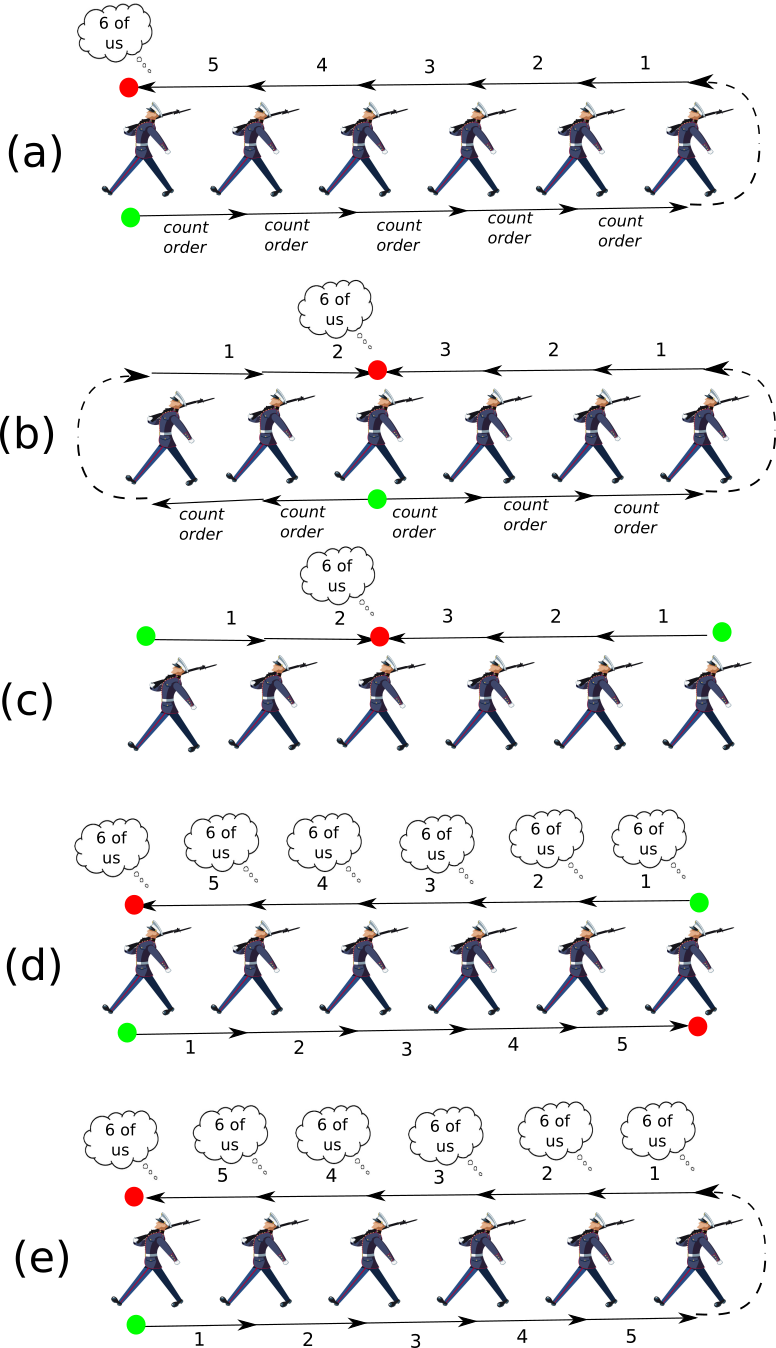
\includegraphics[width=4in]
{mpass/soldiers.png}
\caption{Distributed soldier counting 
(This example
comes from Chapter 4 of
Ref.\cite{pearl-1988book}). 
Green dots indicate the
beginning and red dots the end
of a count. Only
first soldier can calculate
total count in (a). Only 
third soldier can calculate total count
in (b,c). 
All soldiers can calculate
the total count in 
(d,e). One starting point
in (a,b,e).
Two ends as starting points
in (c,d).
} 
\label{fig-soldiers}
\end{figure}

\section{Spring Systems}


\begin{figure}[h!]
\centering
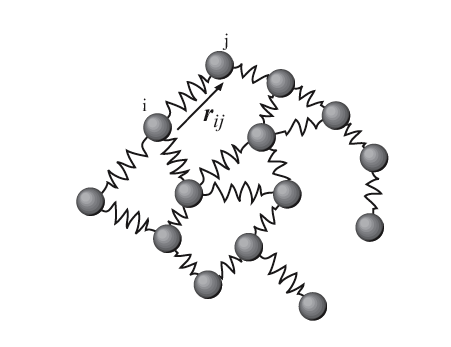
\includegraphics[width=3in]
{mpass/spring-net.png}
\caption{Spring system.
Point masses connected by springs.}
\label{fig-sping-net}
\end{figure}

\begin{figure}[h!]
\centering
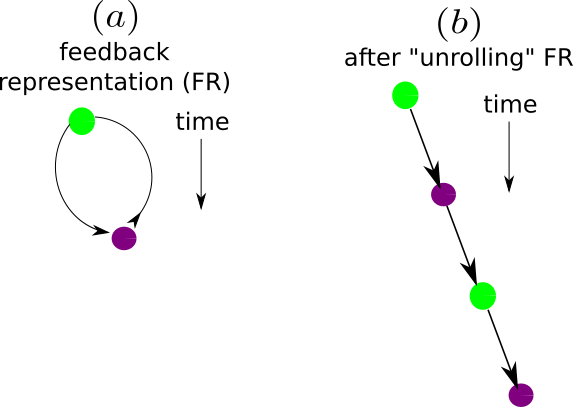
\includegraphics[width=2.7in]
{mpass/time-travel.png}
\caption{Diagram $(a)$ portrays two events interacting via feedback. Diagram $(b)$
represents the same thing as diagram $(a)$
after \qt{unrolling} it.}
\label{fig-time-travel}
\end{figure}

See Ref.\cite{wiki-spring-net}
for an introduction to spring systems.
Ideal springs between the point mass
nodes would
not be sufficient.
One would have to add damping to
the springs so as
to reach an equilibrium.
Time dependent forces (loads)
pointing into or out of the page, applied
to the point masses, would
generate signals that would
propagate
like BP messages.


The messages in Fig.\ref{fig-time-travel} $(a)$
appear to travel both forward and backwards in time.
But in reality, messages cannot travel backward in time.  Fig.\ref{fig-time-travel} $(a)$
is just a convenient representation of
Fig.\ref{fig-time-travel} $(b)$, which \qt{unrolls} it. Both $(a)$ and $
(b)$ are representations of feedback.
Messages that appear to travel back in time,
(but in reality don't, this are just a convenient
representation of feedback)
is a recurring theme in Physics. For example,
in Quantum Electrodynamics, it appears that positrons can travel backwards in time.  In reality,
they are portraying the feedback mechanism whereby two
charged
particles
apply a force on each other.


\section{BP for Markov Chains}

\hrule
Notation:

$\rva\rdart\rvb$ and $\rvb\ldart\rva$ will mean the same thing, namely either a dot or dashed
message arrow, but not a bnet arrow.

$\pi_{\rvb\ldart\rva}(a) = P(a|\eps^-)$

$\lam_{\rvb\rdart\rva}(b) = P(\eps^+|b)$

Note that the argument of 
$\pi_{\rvb\ldart\rva}(a)$ and
$\lam_{\rvb\rdart\rva}(b)$ is the node at
the starting end of the double arrow.

The $\pi$  messages
(probability functions)
travel downstream (i.e., 
they carry info
in the direction
of the graph arrows, towards the future)
and are indicated by a dashed arrow
or by a left double arrow $\ldart$. 
The $\lam$  messages 
(likelihood functions) travel 
upstream (i.e., they 
carry info opposite to 
direction of the graph arrows,
towards the past)
and are indicated
by a dotted arrow
or by a right double arrow $\rdart$.
$\rveps^+$
stands for future evidence and 
$\rveps^-$ for past evidence. 
\hrule



Note that Bayes rule would affirm
 that\footnote{As usual in this book,
$\caln(!x)$ means
a constant that is independent of $x$.}

\beq
P(x|\eps^+)=
\caln(!x)
\underbrace{P(\eps^+|x)}_
{\lam_{\rveps^+\rdart \rvx}(x)}
P(x)
\;.
\eeq
Thus, Eq.(\ref{eq-2-sided-bayes})
is like a 2-sided Janus Bayes rule.

Note that the $\pi$ messages and
$\lam$ messages propagate 
independently
of each other, via the 
 TPM $P(x|\eps^-)$:

\begin{subequations}
\beq
\underbrace{\pi_{\rveps^+\ldart\rvx}(x)}_
{P(x|\eps^-_0)}
=\sum_{\eps^-}P(x|\eps^-)
\underbrace{\pi_{\rvx\ldart \rveps^-}(\eps^-)}_
{\delta(\eps^-, \eps^-_0)}
\eeq

\beq
\underbrace{
\lam_{\rvx\rdart \rveps^-}(\eps^-)}_
{P(\eps^+|\eps^-)}
=
\sum_x P(x|\eps^-)
\underbrace{
\lam_{\rveps^+\rdart \rvx}(x)}_
{P(\eps^+|x)}
\eeq
\label{eq-pi-lam-propagate}
\end{subequations}

Eqs.(\ref{eq-pi-lam-propagate})
suggest that we define an edge bnet
for the $\pi$ and $\lam$
messages (these messages
live in the edges
between the nodes
$\rveps^+, \rvx, \rveps^-$).
Such an edge bnet, shown
in Fig.\ref{fig-BEL-2pi}, is 
complementary to 
bnet for the nodes themselves.
We will call it
the {\bf BP 2-track bnet}
for the bnet Fig.\ref{fig-mp-3chain},
because it has two \qt{tracks},
one for $\pi$ messages and another
for $\lam$ ones.
The TPMs, printed in blue,
for bnet
Fig.\ref{fig-BEL-2pi}, are 
as follows:

\begin{figure}[h!]
$$\xymatrix{
&\ul{\pi}_{\rveps^+\ldart\rvx}\ar[dr]
&&\ul{\pi}_{\rvx\ldart\rveps^-}\ar[ll]
\\
&&\rvB_\rvx
\\
&\ul{\lam}_{\rveps^+\rdart\rvx}\ar[rr]\ar[ru]
&&\ul{\lam}_{\rvx\rdart\rveps^-}
}$$
\caption{BP 2-track
bnet for the bnet
 Fig.\ref{fig-mp-3chain}.}
\label{fig-BEL-2pi}
\end{figure}


\hrule

\begin{figure}[h!]
$$\xymatrix{
\rveps^+
\ar@{<--}@<2ex>[rr]^{\pi_{\rveps^+\ldart\rvb}}
\ar@{.>}@<-2ex>[rr]_{\lam_{\rveps^+\rdart\rvb}}
&&
\rvb\ar[ll]
\ar@{<--}@<2ex>[rr]^{\pi_{\rvb\ldart\rvx}}
\ar@{.>}@<-2ex>[rr]_{\lam_{\rvb\rdart\rvx}}
&&
\rvx\ar[ll]
\ar@{<--}@<2ex>[rr]^{\pi_{\rvx\ldart\rva}}
\ar@{.>}@<-2ex>[rr]_{\lam_{\rvx\rdart\rva}}
&&
\rva\ar[ll]
\ar@{<--}@<2ex>[rr]^{\pi_{\rva\ldart\rveps^-}}
\ar@{.>}@<-2ex>[rr]_{\lam_{\rva\rdart\rveps^-}}
&&
\rveps^-\ar[ll]
}$$
\caption{5 node Markov chain}
\label{fig-mp-5chain}
\end{figure}

So far in 
this section, we have considered Markov
chains with 3 nodes.
Before 
concluding our
discussion of BP for Markov chains,
let us consider BP
for a slightly longer chain.
Let us consider
the 5 node Markov
chain
$\rveps^+\larrow\rvb\larrow\rvx\larrow\rva\larrow\rveps^-$
shown in Fig.\ref{fig-mp-5chain}.
We have already dealt 
with the end nodes
of a Markov chain in the 
3 node Markov chain
example above,
so in the 
5 node case, let us
focus on the internal (i.e., not at
an end) node $\rvx$ and its neighbors
$\rva$ and $\rvb$. Define



\beq
\begin{array}{l|l|l|l}
\pi_{\rveps^+\ldart \rvb}(b)=
P(b|\eps^-)
&
\pi_{\rvb\ldart \rvx}(x)=
P(x|\eps^-)
&
\pi_{\rvx\ldart \rva}(a)=
P(a|\eps^-)
&
\pi_{\rva\ldart \rveps^-}(\eps^-)=
P(\eps^-|\eps^-)
\\
\lam_{\rveps^+\rdart \rvb}(\eps^+)=
P(\eps^+|\eps^+)
&
\lam_{\rvb\rdart \rvx}(b)=
P(\eps^+|b)
&
\lam_{\rvx\rdart \rva}(x)=
P(\eps^+|x)
&
\lam_{\rva\rdart \rveps^-}(a)=
P(\eps^+|a)
\end{array}
\eeq


In analogy
with the case of BP for a
P(\pi_{\rvb\ldart\rvx}|\pi_{\rvx\ldart\rva})=
\prod_{x}\indi\left(
\pi_{\rvb\ldart\rvx}(x)=\sum_a P(x|a)
\pi_{\rvx\ldart\rva}(a)
 3 node Markov
chain, we can define the bnet
Fig.\ref{fig-BEL-4pi},
which we refer to as the
{\bf BP
2-track bnet} for Fig.\ref{fig-mp-5chain}.
The TPMs, printed in blue,
 for bnet Fig.\ref{fig-BEL-4pi}, are
as follows:





\begin{figure}[h!]
$$\xymatrix{
&\ul{\pi}_{\rveps^+\ldart\rvb}\ar[dr]
&&\ul{\pi}_{\rvb\ldart\rvx}\ar[ll]\ar@[red][dr]
&&\ul{\pi}_{\rvx\ldart\rva}\ar@[red][ll]\ar[dr]
&&\ul{\pi}_{\rva\ldart\rveps^-}\ar[ll]
\\
&&\rvB_\rvb
&&\rvB_\rvx
&&\rvB_\rva
\\
&\ul{\lam}_{\rveps^+\rdart\rvb}\ar[rr]
&&\ul{\lam}_{\rvb\rdart\rvx}
\ar@[red][rr]\ar[ul]
&&\ul{\lam}_{\rvx\rdart\rva}\ar[rr]\ar@[red][ul]
&&\ul{\lam}_{\rva\rdart\rveps^-}\ar[ul]
}$$
\caption{BP 2-track bnet for the bnet
Fig.\ref{fig-mp-5chain}.}
\label{fig-BEL-4pi}
\end{figure}


\beq\color{blue}
P(\pi_{\rvb\ldart\rvx}|\pi_{\rvx\ldart\rva})=
\prod_{x}\indi\left(
\pi_{\rvb\ldart\rvx}(x)=\sum_a P(x|a)
\pi_{\rvx\ldart\rva}(a)
\right)
\label{eq-pr-pi-bar-pi}
\eeq

\beq\color{blue}
P(\lam_{\rvx\rdart \rva}|
\lam_{\rvb\rdart \rvx})=
\prod_{a}
\indi\left(
\lam_{\rvx\rdart \rva}(a)
=
\sum_x P(x|a)
\lam_{\rvb\rdart \rvx}(x)
\right)
\label{eq-pr-lam-bar-lam}
\eeq

\beq\color{blue}
P(B_\rvx|
\pi_{\rvb\ldart \rvx},
\lam_{\rvx\rdart \rva})=
\prod_x
\indi\left(
B_\rvx(x)=BEL_\rvx(x)
\right)
\eeq



Let us represent the Markov
chain of Fig.\ref{fig-mp-5chain}
by
$\rvx_{nx-1}
\larrow \ldots, \rvx_2\larrow \rvx_1\larrow \rvx_0$
where $nx=5$.
For any node 
$\rvx_i$
with
parent $\ul{px}_i=\rvx_{i-1}$
and child $\ul{cx}_i=\rvx_{i+1}$, 
define
the {\bf memory matrix}
$\calm_{\rvx_i}$
for node $\rvx_i$
as

\beq
\calm_{\rvx_i}=
[
\calm^+_{\rvx_i},
\calm^-_{\rvx_i}]
\;,
\eeq
where $+=$future, $-=$past, and 

\beq
\calm^+_{ \rvx_i}=
\left[
\begin{array}{c}
\pi_{\ul{cx}_i\ldart \rvx_i}(\cdot)
\\
\lam_{\ul{cx}_i\rdart \rvx_i}(\cdot)
\end{array}
\right]
\;, 
\;\;\;
\calm^-_{\rvx_i}=
\left[
\begin{array}{c}
\pi_{\rvx_i \ldart \ul{px}_i}(\cdot)
\\
\lam_{\rvx_i \rdart \ul{px}_i}(\cdot)
\end{array}
\right]
\;.
\eeq 
Note that

\beq
\calm^-_{\rvx_i}=
\calm^+_{\ul{px}_i}
\label{eq-mem-overlap}
\eeq
for all nodes $\rvx_i$.
We will refer to
Eqs.(\ref{eq-mem-overlap}) as
the {\bf memory overlap
conditions}.

We will also use a permuted version of the 
memory matrix

\beq
\calm'_{\rvx_i}=
[
\calm^{OUT}_{\rvx_i},
\calm^{IN}_{\rvx_i}]
\;,
\eeq
where

\beq
\calm^{OUT}_{ \rvx_i}=
\left[
\begin{array}{c}
\pi_{\ul{cx}_i\ldart \rvx_i}(\cdot)
\\
\lam_{\rvx_i \rdart \ul{px}_i}(\cdot)
\end{array}
\right]
\;, 
\;\;\;
\calm^{IN}_{\rvx_i}=
\left[
\begin{array}{c}
\pi_{\rvx_i \ldart \ul{px}_i}(\cdot)
\\
\lam_{\ul{cx}_i\rdart \rvx_i}(\cdot)
\end{array}
\right]
\;.
\eeq

\begin{figure}[h!]
$$\xymatrix{
\ucalm_{\rveps^+}
&
\ucalm_\rvb\ar[l]
&
\ucalm_\rvx\ar[l]
&
\ucalm_\rva\ar[l]
&
\calm_{\rveps^-}\ar[l]
}$$
\caption{BP Memory Bnet for the bnet
Fig.\ref{fig-mp-5chain}. }
\label{fig-mem-5chain}
\end{figure}

Unfortunately,
2-track bnets cannot be
 generalized in any
obvious way  from 
Markov chains to more
complicated DAGs.
An alternative to 2-track bnets
that still
carries message
info in its nodes,
are memory bnets. An BP
{\bf memory bnet}
is a bnet 
which takes each node
of an original
bnet and
adds a local memory to it.
More specifically,
it keeps that DAG
but replaces each node
$\rvx_i$
by a memory $\ucalm_{\rvx_i}$.
Fig.\ref{fig-mem-5chain} shows 
the memory bnet for
the bnet Fig.\ref{fig-mp-5chain}.
The TPM, printed in blue,
for the  node $\ucalm_\rvx$
of the memory bnet 
Fig.\ref{fig-mem-5chain}, is as follows

\beq\color{blue}
P(\calm_{\rvx_i}|
\calm_{\rvn\in nb(\rvx_i)}
)= A B
\;,
\eeq
where

\beq
A=
\indi(\calm^{-}_{\rvx_i}=\calm^{+}_{\ul{px}_i})
\;,
\eeq
and

\beq
B=
\indi(\calm^{OUT}_{\rvx_i}=\calc(\calm^{IN}_{\rvx_i}))
\label{eq-mp-update-static}
\;.
\eeq
The function $\calc$,
which 
we will call the {\bf BP local computation},
maps $\calm^{IN}_{\rvx_i}$
into $\calm^{OUT}_{\rvx_i}$. More explicitly,
$\calc$ is defined so that

\beq
B
=
\underbrace{P(\pi_{\rvb\ldart\rvx}|
\pi_{\rvx\ldart\rva})}_{B_\pi}
\underbrace{P(\lam_{\rvx\rdart \rva}|
\lam_{\rvb\rdart \rvx})}_{B_\pi}
\;,
\eeq
where
$B_\pi$ and $B_\lam$
are given by Eqs.(\ref{eq-pr-pi-bar-pi})
and (\ref{eq-pr-lam-bar-lam}),
respectively.



The BP memory bnet
 Fig.
\ref{fig-mem-5chain}
is a deterministic bnet.
A deterministic bnet
is basically
just a coupled system
of equations (CSE)
for some unknowns $x_i$. 
A CSE per se does not
include with it a method for  
solving for the $x_i$. Such methods are not
unique.
For example,
for the 
distributed
soldier counting 
problem,
the various 
methods that
we described
for counting soldiers
are just different
methods 
for solving the same
CSE.
One can describe 
a method for solving a
CSE using a dynamical bnet.\footnote{
The term
dynamical bnet
was used in Chapter \ref{ch-dyn-bnets}
to mean a time inhomogeneous
Markov chain, but 
here we are stretching its meaning to
include
Markov chains
that aren't 
time inhomogeneous.}
To solve
the CSE
represented by
the memory bnet Fig.\ref{fig-mem-5chain},
we will use the 
dynamical bnet
Fig.\ref{fig-propagation-5chain}.
Henceforth, 
we will refer to
Fig.\ref{fig-propagation-5chain} as
an {\bf BP dynamical bnet}
for Fig.\ref{fig-mem-5chain}.

\begin{figure}
$$\xymatrix{
\rveps^-\ar[d]
&\ucalm^{(0)}_{\rveps^-}\ar[r]\ar[dr]
&\ucalm^{(1)}_{\rveps^-}\ar[r]
&\ucalm^{(2)}_{\rveps^-}\ar[r]
&\ucalm^{(3)}_{\rveps^-}\ar[r]
&\ucalm^{(4)}_{\rveps^-}
&
\\
\rva\ar[d]
&\ucalm^{(0)}_{\rva}\ar[r]
&\ucalm^{(1)}_{\rva}\ar[r]\ar[dr]
&\ucalm^{(2)}_{\rva}\ar[r]
&\ucalm^{(3)}_{\rva}\ar[r]\ar[ur]
&\ucalm^{(4)}_{\rva}
\\
\rvx\ar[d]
&\ucalm^{(0)}_{\rvx}\ar[r]
&\ucalm^{(1)}_{\rvx}\ar[r]
&\ucalm^{(2)}_{\rvx}\ar[r]\ar[dr]\ar[ur]
&\ucalm^{(3)}_{\rvx}\ar[r]
&\ucalm^{(4)}_{\rvx}
\\
\rvb\ar[d]
&\ucalm^{(0)}_{\rvb}\ar[r]
&\ucalm^{(1)}_{\rvb}\ar[r]\ar[ur]
&\ucalm^{(2)}_{\rvb}\ar[r]
&\ucalm^{(3)}_{\rvb}\ar[r]\ar[dr]
&\ucalm^{(4)}_{\rvb}
\\
\rveps^+
&\ucalm^{(0)}_{\rveps^+}\ar[r]\ar[ur]
&\ucalm^{(1)}_{\rveps^+}\ar[r]
&\ucalm^{(2)}_{\rveps^+}\ar[r]
&\ucalm^{(3)}_{\rveps^+}\ar[r]
&\ucalm^{(4)}_{\rveps^+}
}$$
\caption{BP dynamical bnet for the bnet
  Fig.\ref{fig-mem-5chain}.}
\label{fig-propagation-5chain}
\end{figure}

\begin{figure}[h!]
$$
\xymatrix{
\rveps^+\ar@[red]@{.>}@<-2ex>[r]
&\rvb\ar[l]
&\rvx\ar[l]
&\rva\ar[l]
&\rveps^-\ar[l]\ar@[red]@{-->}@<-2ex>[l]
\\
\rveps^+
&\rvb\ar[l]\ar@[red]@{.>}@<-2ex>[r]
&\rvx\ar[l]
&\rva\ar[l]\ar@[red]@{-->}@<-2ex>[l]
&\rveps^-\ar[l]
\\
\rveps^+
&\rvb\ar[l]
&\rvx\ar[l]\ar@[red]@{.>}@<-2ex>[r]
\ar@[red]@{-->}@<-2ex>[l]
&\rva\ar[l]
&\rveps^-\ar[l]
\\
\rveps^+
&\rvb\ar[l]\ar@[red]@{-->}@<-2ex>[l]
&\rvx\ar[l]
&\rva\ar[l]\ar@[red]@{.>}@<-2ex>[r]
&\rveps^-\ar[l]
}$$
\caption{
Steps encoded in the 
bnet 
Fig.\ref{fig-propagation-5chain}.
Note the 
similarity 
of this figure 
to Fig.\ref{fig-soldiers} (d)
for soldier counting.
} 
\label{fig-multiframe-5chain}
\end{figure}

Next, we will
explain the meaning
of Fig.\ref{fig-propagation-5chain}.
Fig.\ref{fig-propagation-5chain}
is a step by step
recipe (i.e., algorithm)
for solving a CSE,
where the unknowns are
memory matrices.
Each step
encoded in
Fig.\ref{fig-propagation-5chain}
corresponds to a
specific
message sending event,
where the messages
are sent
along the edges 
of the Markov chain
Fig.\ref{fig-mp-5chain}.
These message sending
events are portrayed in
chronological order
in Fig.\ref{fig-multiframe-5chain}.
In that figure,
$\pi$ messages
are indicated by
dashed red arrows,
and $\lam$ messages
by dotted red arrows.  
These steps, or
message  sending events,
lead to an updating
of the memory matrices
that we are solving for.
Each step propagates information
between the memory nodes.
In the usual Pearl BP algo, 
the evidence nodes 
initiate the BP
chain of 
message passing events.
These events 
continue
until 
the 
memory 
matrices
reach an equilibrium
and the CSE is solved.


To use
bnet 
Fig.\ref{fig-propagation-5chain},
we need to specify
the {\bf initial conditions}
(i.e., the value of 
$\calm^{(0)}_{\rvx_i}$ 
for all $i$).
For that, one can use

\beq
\pi^{(0)}_{\ul{px}_0\ldart \rvx_0}
=
P(x_0)
\;,
\eeq

\beq
\lam^{(0)}_{\ul{cx}_i\rdart\rvx_{nx-1}}(x_{nx-1})
=
\delta(x_{nx-1}, x'_{nx-1})
\;.
\eeq
All other $\calm^{(0)}_{\rvx_i}$ entries
for all $i$ can be set to 1.

The TPMs, printed in blue, for
bnet Fig.\ref{fig-propagation-5chain},
are as follows.

\beq\color{blue}
P(\calm^{(t)}_{\rvx_i}|
\calm^{(t-1)}_{\rvn\in nb(\rvx_i)},
\calm^{(t-1)}_{\rvx_i}
)= A B
\;,
\eeq
where

\beq
A=\left\{
\begin{array}{ll}
\indi(\calm^{(t)-}_{\rvx_i}=\calm^{(t-1)+}_{\ul{px}_i})
&\text{ if input from $\ul{px}_i$}
\\
\\
\indi(\calm^{(t)+}_{\rvx_i}=\calm^{(t-1)-}_{\ul{cx}_i})
&\text{ if input from $\ul{cx}_i$}
\end{array}
\right.
\;,
\eeq
and

\beq
B=
\indi(\calm^{(t)OUT}_{\rvx_i}=\calc(\calm^{(t)IN}_{\rvx_i}))
\label{eq-mp-update}
\;.
\eeq
The function $\calc$,
which 
we will call the {\bf BP local computation},
maps $\calm^{(t)IN}_{\rvx_i}$
into $\calm^{(t)OUT}_{\rvx_i}$. More explicitly,
$\calc$ is defined so that

\beq
B
=
B_\pi B_\lam
\eeq
where

\beq
B_\pi=
\prod_{x}\indi\left(
\underbrace{\pi^{(t)}_{\rvb\ldart\rvx}(x)}_
{OUT}
=\sum_a P(x|a)
\underbrace{\pi^{(t)}_{\rvx\ldart\rva}(a)}_{IN}
\right)
\eeq
and

\beq
B_\lam=
\prod_{a}
\indi\left(
\underbrace{\lam^{(t)}_{\rvx\rdart \rva}(a)}_{OUT}
=
\sum_x P(x|a)
\underbrace{\lam^{(t)}_{\rvb\rdart \rvx}(x)}_{IN}
\right)
\;.
\eeq

The basic idea behind Eq.(\ref{eq-mp-update}),
which we will call the
{\bf memory updating equation}, is simple:
the memory overlap conditions translate the information
from time $t-1$ to $t$, and
then the local computation translates 
$IN$ to $OUT$ at fixed time $t$.




\section{BP Algorithm for Polytrees}


Consider Fig.\ref{fig-pi-lam},
which illustrates
a bnet node $\rvx$ receiving and sending
messages to its neighbors.
The $\pi$  messages
(probability functions)
travel downstream (i.e., 
they carry info
in the direction
of the graph arrows, towards the future)
and are indicated by a dashed arrow
or by a left double arrow $\ldart$. 
The $\lam$  messages 
(likelihood functions) travel 
upstream (i.e., they 
carry info opposite to 
direction of the graph arrows,
towards the past)
and are indicated
by a dotted arrow
or by a right double arrow $\rdart$.

Note that argument $arg$ of the $\pi(arg)$
and $\lam(arg)$
functions is always the same
as the letter in the subscript
that is closest to the argument.

Note that in Fig.\ref{fig-pi-lam},
we indicate
messages that travel
\qt{downstream}
(resp., \qt{upstream}), by
arrows with dashed (resp., dotted)
 lines as shafts.
Mnemonic: think of the shaft as a
 velocity vector field
for the message.
You travel faster when
you swim downstream as opposed
to upstream.

$pa(\rvx)=$ parents of node $\rvx$

$ch(\rvx)=$ children of node $\rvx$

$nb(\rvx)=pa(\rvx)\cup ch(\rvx)=$
neighbors of node $\rvx$



\begin{figure}[h!]
\centering
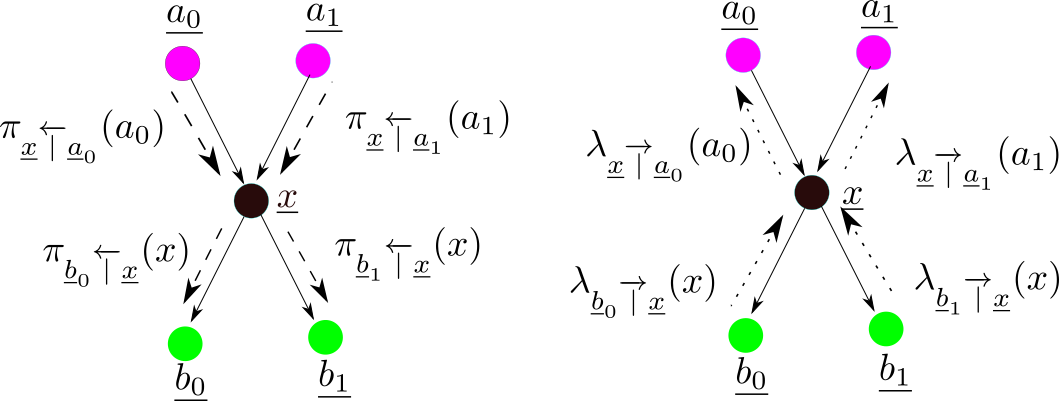
\includegraphics[width=6in]{mpass/pi-lam.png}
\caption{Node $\rvx$ receiving
and sending messages to
 its neighbors. (neighbors=
parents and children).
}
\label{fig-pi-lam}
\end{figure}


We define a {\bf memory matrix}
$\calm_{\rvx}$ for node $\rvx$
as

\beq
\calm_{\rvx}=
[
\calm^+_{\rvx},
\calm^-_{\rvx}]
\;,
\eeq
where $+=$future, $-=$past, and 

\beq
\calm^+_{ \rvx}=
\left[
\begin{array}{cc}
\pi_{\rvb\ldart\rvx}(\cdot)
&
\lam_{\rvb\rdart\rvx}(\cdot)
\end{array}
\right]_{\rvb\in ch(\rvx)}
=[\calm^+_{\rvb, \rvx}]_{\rvb\in ch(\rvx)}
\;,
\eeq

\beq
\calm^-_{\rvx}=
\left[
\begin{array}{c}
\pi_{\rvx\ldart\rva}(\cdot)
\\
\lam_{\rvx\rdart\rva}(\cdot)
\end{array}
\right]_{\rva\in  pa(\rvx)}
=[\calm^-_{\rvx, \rva}]_{\rva\in pa(\rvx)}
\;.
\eeq 
Note that

\beq
\calm^-_{\rvx, \rva}=
\calm^+_{\rva, \rvx}
\label{eq-mem-overlap-poly}
\eeq
for every arrow $\rvx\larrow\rva$.
We will refer to
Eqs.(\ref{eq-mem-overlap-poly}) as
the {\bf memory overlap
conditions}.

We will also use a permuted version of the 
memory matrix

\beq
\calm'_{\rvx}=
[
\calm^{OUT}_{\rvx},
\calm^{IN}_{\rvx}]
\;,
\eeq
where

\beq
\calm^{OUT}_{ \rvx}=
\left(
\begin{array}{c}
[\pi_{\rvb\ldart\rvx}(\cdot)]_
{\rvb\in ch(\rvx)}
\\
{[}\lam_{\rvx\rdart\rva}(\cdot)]_
{\rva\in  pa(\rvx)}\;,
\end{array}
\right)
\\
=
[\calm^{OUT}_{\rvx,\rvn}]_{\rvn\in nb(\rvx)}
\;, 
\eeq

\beq
\calm^{IN}_{\rvx}=
\left(
\begin{array}{c}
[\pi_{\rvx\ldart\rva}(\cdot)]_
{\rva\in  pa(\rvx)}
\\
{[}\lam_{\rvb\rdart\rvx}(\cdot)]_
{\rvb\in ch(\rvx)}
\end{array}
\right)
\\
=
[\calm^{IN}_{\rvx,\rvn}]_{\rvn\in nb(\rvx)}
\;.
\eeq


\hrule

For times $t=0, 1, \dots, T-1$,
 we calculate $\calm^{(t)}_\rvx$ in
two steps: first we calculate $\calm^{(t)IN}_\rvx$
from earlier memories at time $t-1$,
 then
we calculate $\calm^{(t)OUT}_\rvx$:

\begin{figure}[h!]
\centering
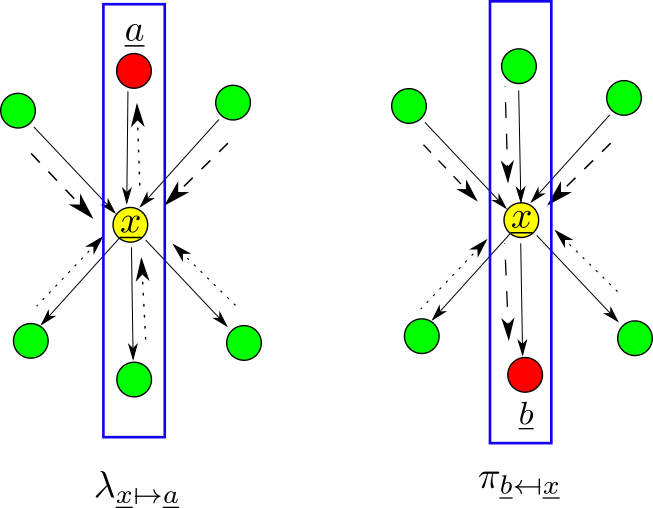
\includegraphics[width=3.5in]
{mpass/mpass-messages.png}
\caption{
Subgraph of a bnet
showing two cases (RULE 1
 and RULE 2)
of message info flow.
The yellow
node is a gossip monger.
It receives messages from
all the green nodes,
and then it relays a joint
message to the red node.
Union of green nodes and the red node = full
 neighborhood of yellow node.
There are two possible
cases: the
red node is either a parent
or a child of the yellow
one. As usual, we use arrows with
dashed (resp., dotted) shafts for
downstream (resp., upstream) messages. 
Blue boxes indicate Markov chain case. }
\label{fig-messages-gen}
\end{figure}

An {\bf evidence node} is a
node whose TPM is a delta function
set to a particular state of the node. 
We will assume, without loss of generality,
that all evidence nodes are leaf nodes.
If that is not the case, 
any
evidence node $\rve$
that is not
a leaf node,
can be given a new
companion leaf node $\rvl$
connected to $\rve$ by 
an arrow $\rvl\larrow \rve$,
and such that
$\rvl$ has a delta
function TPM.



\begin{enumerate}
\item {\bf Calculating
$\calm^{(t)IN}_\rvx$
from signals received from
 $\rvn\in nb(\rvx)$, sent at earlier time $t-1$:}

Set

\beq
\calm^{(t)-}_{\rvx, \rva}|_\pi=
\calm^{(t-1)+}_{\rva, \rvx}|_\pi
\;,
\eeq
for all $\rva\in pa(\rvx)$,
and 
\beq
\calm^{(t)+}_{\rvb, \rvx}|_\lam=
\calm^{(t-1)-}_{\rvx, \rvb}|_\lam
\;,
\eeq
for all $\rvb\in ch(\rvx)$.
By $X|_\lam$ (resp., $X|_\pi$)
we mean the $\lam$ (resp., $\pi$)
component of $X$.

\item {\bf Calculating $\calm^{(t)OUT}_\rvx$
from already calculated $\calm^{(t)IN}_\rvx$:}

Let $\rva^{na}=
(\rva_i)_{i=0, 1, \ldots, na-1}$
denote the parents of $\rvx$
and
$\rvb^{nb}=
(\rvb_i)_{i=0, 1, \ldots, nb-1}$
its children.

Define

\beqa
\label{eq-mp-pix}
\pi_\rvx(x)&=&
\sum_{a^{na}} P(x|a^{na})
\prod_i
\pi_{\rvx\ldart\rva_i}
(a_i)\\
&=&E_{\rva^{na}}[P(x|a^{na})]
\eeqa
(boundary case: if $\rvx$
is a root node, use $\pi_\rvx(x)=P(x)$.)
and

\beq
\lam_\rvx(x)=
\prod_i
\lam_{\rvb_i\rdart \rvx}(x)
\;.
\label{eq-mp-lamx}
\eeq
(boundary case: if $\rvx$
is a leaf node, use $\lam_\rvx(x)=1$.)
\begin{itemize}

\item{\bf RULE 1: (red parent)}

From
the $\lam_{\rvx \rdart\rva}$
panel of Fig.\ref{fig-messages-gen},
 we get

\begin{align}
\label{eq-mp-rule1}
\underbrace{\lam_{\rvx\rdart\rva_i}
(a_i)}_{OUT}&=
\caln(!a_i)
\sum_x\left[
\underbrace{\lam_\rvx(x)}_{IN}
\sum_{(a_k)_{k\neq i}}\left(
P(x|a^{na})\prod_{k\neq i}
\underbrace{\pi_
{\rvx\ldart\rva_k}
(a_k)}_{IN}
\right)\right]
\\&=
\caln(!a_i)
\sum_x\left[
\lam_\rvx(x)
E_{(\rva_k)_{k\neq i}}[P(x|a^{na})]\right]
\\&=
\caln(!a_i)
E_{(\rva_k)_{k\neq i}}E_{\rvx|a^{na}}
\lam_\rvx(x)
\end{align}
(boundary case:
if $\rvx$ is a root node, use
$\lam_{\rvx\rdart\rva_i}
(a_i)=\caln(!a_i)$.)

\item{\bf RULE 2: (red child)}

From the $\pi_{\rvb \ldart\rvx}$
panel of
Fig.\ref{fig-messages-gen},
we get


\beq
\underbrace{\pi_{\rvb_i\ldart\rvx}
(x)}_{OUT}=
\caln(!x)
\underbrace{\pi_\rvx(x)}_{IN}
\prod_{k\neq i}
\underbrace{\lam_{\rvb_k\rdart \rvx}(x)}_{IN}
\label{eq-mp-rule2}
\eeq
(boundary case:
if $\rvx$ is a leaf node, use
$\pi_{\rvb_i\ldart\rvx}(x)=
\caln(!x)\pi_\rvx(x)$
.)

\end{itemize}
\end{enumerate}
In the above
equations, if the
range set of a product is empty, then
 define the product as 1; i.e.,
$\prod_{k\in \emptyset}F(k)=1$.


\hrule\noindent
{\bf Claim:} Define

\beq
BEL^{(t)}(x)=\caln(!x)
\lam^{(t)}_\rvx(x)
\pi^{(t)}_\rvx(x)
\;.\eeq
Then

\beq
\lim_{t\rarrow \infty}BEL^{(t)}(x)=P(x|\eps)
\;.
\eeq
This  says that
the belief in $\rvx=x$
converges to $P(x|\eps)$ and it
equals the product
of messages received from all
parents and children of $\rvx=x$.

\subsection{How BP algo
for polytrees reduces to the 
BP algo for Markov chains}

It is instructive
to see
how the
BP algo
for polytrees reduces to 
BP algo for Markov chains.

For a Markov chain, node
$\rvx$ has a single parent (i.e., ancestor) $\rva$
and a single child $\rvb$.

Therefore, 
Eqs.(\ref{eq-mp-pix}) and (\ref{eq-mp-lamx}) reduce to

\beq
\pi_\rvx(x)=
\sum_a
P(x|a)\pi_{\rvx\ldart\rva}(a)
\eeq
and

\beq
\lam_\rvx(x)=
\lam_{\rvb\rdart \rvx}(x)
\;.
\eeq

RULE 1 given by Eq.(\ref{eq-mp-rule1}) reduces to

\beqa
\lam_{\rvx\rdart \rva}(a)
&=&
\caln(!a)\sum_x
\lam_\rvx(x)P(x|a) 
\\
&=&
\caln(!a)\sum_x
\lam_{\rvb\rdart \rvx}(x)P(x|a) 
\eeqa

RULE 2 given by Eq.(\ref{eq-mp-rule2}) reduces to

\beqa
\pi_{\rvb\ldart \rvx}(x)
&=&
\caln(!x)\pi_\rvx(x)
\\
&=&
\sum_a
P(x|a)\pi_{\rvx\ldart\rva}(a)
\;.
\eeqa



\section{Derivation of BP Algorithm
for Polytrees}

This derivation is taken from
 the 1988 book Ref.\cite{pearl-1988book}
by Judea Pearl, where it
is presented very lucidly. We only
made some minor
changes in notation.

\hrule\noindent
 {\bf Notation}

The BP algorithm yields an expansion
 for $P(x|\eps)$.

$\rvx$= the focus node,
arbitrary node of bnet that we are
focusing on to calculate its $P(x|\eps)$.



$(\rva_i)_{i=0,1, \ldots, na-1}$. = parent nodes
 (mnemonic: a=ancestor) of $\rvx$

$(\rvb_i)_{i=0,1, \ldots, nb-1}$. =
children nodes of $\rvx$.

$\rveps$= set of nodes for which
 there is evidence; that is,
$\rveps=\eps$, so
the state of these nodes is fixed.


$\rveps^-_\rvx= \rveps\cap an(\rvx)$
(evidence in past of $\rvx$)\footnote{
Careful:
Chapter 4
of Ref.\cite{pearl-1988book}
uses $-$ indicate the future
and $+$ to indicate
 the past. This
is the opposite of our notation.}

$\eps^-_{\rvx \rva_i}=
\eps^-_{\rvx}\cap an(\rva_i)$.

Note that $\eps^-_\rvx=\cup_i 
\eps^-_{\rvx \rva_i}$

$\rveps^+_\rvx= \rveps\cap [de(\rvx)\cup\rvx]$
(evidence in future of $\rvx$)

$\eps^+_{\rvx \rvb_i}=
\eps^+_{\rvx}\cap
 [de(\rvb_i)\cup \rvb_i]$.

Note that $\eps^+_\rvx=\cup_i 
\eps^+_{\rvx \rvb_i}$

Note that $\rveps=\rveps^+_\rvx \cup \eps^-_\rvx$

\beq
\pi_{ \rvx}(x)
=
P(x|\eps^-_\rvx)
\eeq

\beq
\pi_{ \rvx\ldart\rva_i}(a_i)=
P(a_i|\eps^-_{\rvx \rva_i})
\eeq

\beq
\pi_{ \rvb_i\ldart\rvx}(x)=
P(x|\eps^-_{\rvx \rvb_i})
\eeq

\beq
\lam_{\rvx} (x)=P(\eps^+_\rvx|x)
\eeq

\beq
\lam_{\rvb_i\rdart \rvx} (x)=
P(\eps^+_{\rvx \rvb_i}|x)
\eeq

\beq
\lam_{\rvx\rdart \rva_i} (a_i)=
P(\eps^+_{\rvx \rva_i}|a_i)
\eeq


\hrule\noindent
{\bf Expansions
of $\lam_\rvx(x)$ and $\pi_\rvx(x)$
into products of single node messages.}

\beqa
\underbrace{
P(x|\eps^-_\rvx)
}_{\pi_\rvx(x)}
&=&
P(x|\cup_i \eps^-_{\rvx \rva_i})
\\
&=&
\sum_{a^{na}}
P(x|a^{na})
P( a^{na}|\cup_i \eps^-_{\rvx \rva_i})
\\
&=&
\sum_{a^{na}}
P(x|a^{na})
\prod_i
\underbrace{
P(a_i| \eps^-_{\rvx \rva_i})}_{
\pi_{\rvx\ldart \rva_i}(a_i)
}
\eeqa

\beq
\underbrace{
P(\eps^+_\rvx|x)
}_{\lam_\rvx(x)}
=\prod_i
\underbrace{
P(\eps^+_{\rvx \rvb_i}|x)
}_{\lam_{\rvb_i\rdart \rvx}(x)}
\eeq
\hrule

Note that past and future evidences
$\eps^-_\rvx$ and $\eps^+_\rvx$
that are
causally connected to $\rvx$
are
conditionally
independent at fixed $\rvx$:

\beq
P(\eps^+_\rvx, \eps^-_\rvx|x)
=
P(\eps^+_\rvx|x) P(\eps^-_\rvx|x)
\;.
\eeq

This observation is key to the proof of
the following claim:

\begin{claim}
\beqa
P(x| \eps^+_\rvx, \eps^-_\rvx)
&=&
P(\eps^+_\rvx|x) P(x|\eps^-_\rvx
)\frac{1}{P(\eps^+_\rvx|\eps^-_\rvx)}
\\
&=&
\caln(!x)
P(\eps^+_\rvx|x)P(x|\eps^-_\rvx)
\\
&=&
\caln(!x)\;\;\;
(\eps^+_\rvx\larrow x \larrow \eps^-_\rvx)
\\&=&
\caln(!x)
\lam_\rvx (x)
\pi_\rvx(x)
\eeqa


\end{claim}
\proof

\beqa
 P(x|\eps^+_\rvx, \eps^-_\rvx)
&=&
P(\eps^+_\rvx, \eps^-_\rvx|x)\frac{P(x)}{P(\eps^+_\rvx, \eps^-_\rvx)}
\\
&=&
P(\eps^+_\rvx|x) P(\eps^-_\rvx|x)\frac{P(x)}{P(\eps^+_\rvx, \eps^-_\rvx)}
\\
&=&
P(\eps^+_\rvx|x) P(x|\eps^-_\rvx
)\frac{P(\eps^-_\rvx)}{P(\eps^+_\rvx, \eps^-_\rvx)}
\\
&=&
P(\eps^+_\rvx|x) P(x|\eps^-_\rvx
)\frac{1}{P(\eps^+_\rvx|\eps^-_\rvx)}
\eeqa
\qed

Next we prove BP rules 1 and 2.

\begin{itemize}
\item {\bf RULE 1 (red parent)}

\begin{figure}[h!]
\centering
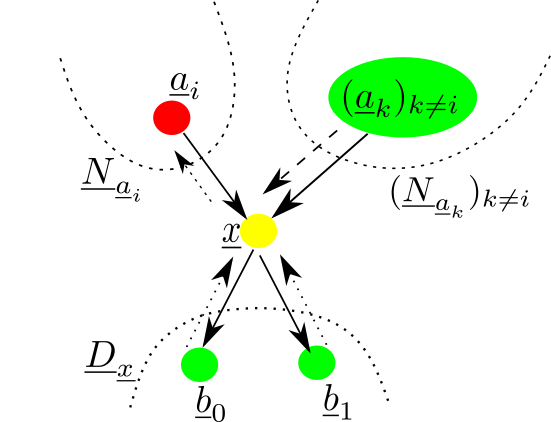
\includegraphics[width=2.65in]
{mpass/mpass-rule-1.png}
\caption{This figure is
used in the derivation of the BP
RULE 1.}
\label{fig-mpass-rule-1}
\end{figure}

Note that

\beqa
\eps^+_\rvx \cup \cup_{k\neq i}\eps^-_{\rvx \rva_k}
&=&
(\eps^+_\rvx\cup \eps^-_\rvx) - \eps^-_{\rvx \rva_i}
\\
&=&
\eps^+_{\rvx \rva_i}
\eeqa

Let $y=(a_k)_{k\neq i}$ and
$\eps^-_\rvy=(\eps^-_{\rvx \rva_k})_{k\neq i}$.

\beqa
\underbrace{
P(\eps^+_{\rvx \rva_i}|a_i)
}_{\lam_{\rvx\rdart\rva_i}(a_i)}
&=&
P(\eps^+_\rvx, \eps^-_\rvy|a_i)
\\
&=&
\sum_x
\sum_y
P(\eps^+_\rvx, \eps^-_\rvy|x,y)
P(x, y|a_i)
\\
&=&
\sum_x
\sum_y
P(\eps^+_\rvx|x)
P(\eps^-_\rvy|y)
P(x|y, a_i )P(y|a_i)
\\
&=&
P(\eps^-_\rvy)
\sum_x
\sum_y
P(\eps^+_\rvx|x)
\frac{P(y|\eps^-_\rvy)}{P(y)}
P(x|y, a_i )
\underbrace{P(y|a_i)}_{=P(y)}
\\
&=&
\caln(!a_i)
\sum_x
\sum_y
P(\eps^+_\rvx|x)
P(x|
\underbrace{
y, a_i
}_{a^{na}}
)P(y|\eps^-_\rvy)
\\
&=&
\caln(!a_i)
\sum_x
\underbrace{
P(\eps^+_\rvx|x)
}_{\lam_{\rvx}(x)}
\sum_{(a_k)_{k\neq i}}
P(x| a^{na})
\prod_{k\neq i}
\underbrace{
P(a_k|\eps^-_{\rvx \rva_k})
}_{\pi_{\rvx\ldart \rva_k}(a_k)}
\eeqa

\item{\bf RULE 2 (red child)}

\begin{figure}[h!]
\centering
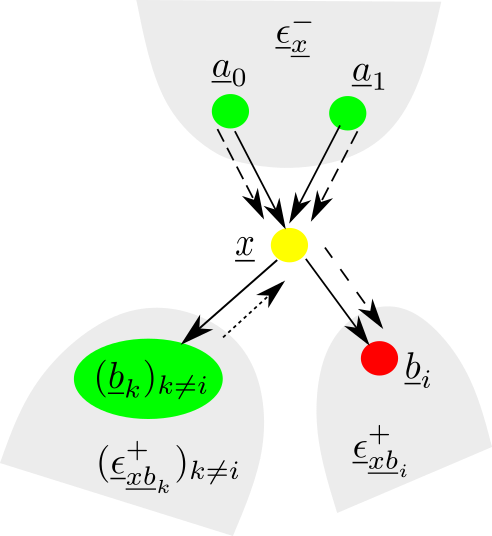
\includegraphics[width=2.5in]
{mpass/mpass-rule-2.png}
\caption{This figure is
used in the derivation of the BP
RULE 2.}
\label{fig-mpass-rule-2}
\end{figure}

Note that

\beqa
(\cup _{k\neq i}
\eps^+_{\rvx \rvb_k})\cup \eps^-_\rvx
&=&
(\eps^+_\rvx\cup \eps^-_\rvx) - \eps^+_{\rvx \rvb_i}
\\
&=&
\eps^-_{\rvx \rvb_i}
\eeqa


\beqa
\underbrace{
P(x| \eps^-_{\rvx \rvb_i})
}_{\pi_{\rvb_i\ldart \rvx}(x)}
&=&
P(x| (\eps^+_{\rvx \rvb_k})_{k\neq i}, \eps^-_\rvx)
\\
&=&
\caln(!x)
P((\eps^+_{\rvx \rvb_k})_{k\neq i}|x)P(x|\eps^-_\rvx)
\\&=&
\caln(!x)
\left(
\prod_{k\neq i}
\underbrace{
P(\eps^+_{\rvx \rvb_k}|x)
}_{\lam_{\rvb_k\rdart\rvx}(x)}
\right)
\underbrace{
P(x|\eps^-_\rvx)
}_{\pi_\rvx(x)}
\eeqa

\end{itemize}


\section{Example of BP algo for a  Tree}

In this section, we 
describe how to apply
the BP algo
to the tree bnet Fig.\ref{fig-mp-9tree}.
In Fig.\ref{fig-mp-9tree}, if we 
replace each integer $i$ by 
the random variable $\rvA_i$,
we get an {\bf original bnet}, 
and if we replace each
$i$
by $\ucalm_{\rvA_i}$,
we get the {\bf BP memory bnet}
of the original bnet.
In Fig.\ref{fig-mp-9tree},
the magenta  nodes are evidence nodes
and the green ones aren't.

We want to solve for the 
memory matrices of the 
memory bnet. To do so,
we use the {\bf BP dynamical bnet}
Fig.\ref{fig-propagation-9tree}.
The steps encoded
in the dynamical bnet
are shown in Fig.\ref{fig-multiframe-9tree}.
Fig.\ref{fig-multiframe-9tree}
has frames in chronological order,
showing the direction of travel
of the $\pi\&\lam$ information. 
This sequence of frames also indicates 
the order
in which we solve for the entries of
 the memory matrices.
The information first emanates from the evidence nodes.
It propagates generally upstream,
although some nodes
can generate downstream flow. Some of the 
info  reaches the root node and is  reflected there.
The root node is the only one that 
is capable of reflection (i.e., instant output
along an arrow, 
in response to input along that arrow).
Eventually, all info
reaches the leaf nodes 
via downstream propagation and is absorbed there.


\begin{figure}[h!]
\centering
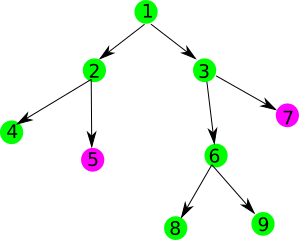
\includegraphics[width=2.5in]
{mpass/mp-9tree.png}
\caption{Example tree bnet
used to illustrate BP.
} 
\label{fig-mp-9tree}
\end{figure}



\begin{figure}[h!]
$$\xymatrix{
\rvA_1 
&\ucalm^{(0)}_{\rvA_1}\ar[r]
&\ucalm^{(1)}_{\rvA_1}\ar[r]
&\ucalm^{(2)}_{\rvA_1}\ar[r]\ar[dr]\ar[ddr]
&\ucalm^{(3)}_{\rvA_1}\ar[r]
&\ucalm^{(4)}_{\rvA_1}\ar[r]
&\ucalm^{(5)}_{\rvA_1}
\\
\rvA_2 
&\ucalm^{(0)}_{\rvA_2}\ar[r]
&\ucalm^{(1)}_{\rvA_2}\ar[r]\ar[ur]\ar[ddr]
&\ucalm^{(2)}_{\rvA_2}\ar[r]
&\ucalm^{(3)}_{\rvA_2}\ar[r]\ar[ddr]\ar[dddr]
&\ucalm^{(4)}_{\rvA_2}\ar[r]
&\ucalm^{(5)}_{\rvA_2}
\\
\rvA_3 
&\ucalm^{(0)}_{\rvA_3}\ar[r]
&\ucalm^{(1)}_{\rvA_3}\ar[r]\ar[uur]\ar[dddr]
&\ucalm^{(2)}_{\rvA_3}\ar[r]
&\ucalm^{(3)}_{\rvA_3}\ar[r]\ar[dddr]\ar[ddddr]
&\ucalm^{(4)}_{\rvA_3}\ar[r]
&\ucalm^{(5)}_{\rvA_3}
\\
\rvA_4 
&\ucalm^{(0)}_{\rvA_4}\ar[r]
&\ucalm^{(1)}_{\rvA_4}\ar[r]
&\ucalm^{(2)}_{\rvA_4}\ar[r]
&\ucalm^{(3)}_{\rvA_4}\ar[r]
&\ucalm^{(4)}_{\rvA_4}\ar[r]
&\ucalm^{(5)}_{\rvA_4}
\\
\rvA_5 
&\ucalm^{(0)}_{\rvA_5}\ar[r]\ar[uuur]
&\ucalm^{(1)}_{\rvA_5}\ar[r]
&\ucalm^{(2)}_{\rvA_5}\ar[r]
&\ucalm^{(3)}_{\rvA_5}\ar[r]
&\ucalm^{(4)}_{\rvA_5}\ar[r]
&\ucalm^{(5)}_{\rvA_5}
\\
\rvA_6 
&\ucalm^{(0)}_{\rvA_6}\ar[r]
&\ucalm^{(1)}_{\rvA_6}\ar[r]
&\ucalm^{(2)}_{\rvA_6}\ar[r]\ar[ddr]\ar[dddr]
&\ucalm^{(3)}_{\rvA_6}\ar[r]
&\ucalm^{(4)}_{\rvA_6}\ar[r]\ar[ddr]\ar[dddr]
&\ucalm^{(5)}_{\rvA_6}
\\
\rvA_7 
&\ucalm^{(0)}_{\rvA_7}\ar[r]\ar[uuuur]
&\ucalm^{(1)}_{\rvA_7}\ar[r]
&\ucalm^{(2)}_{\rvA_7}\ar[r]
&\ucalm^{(3)}_{\rvA_7}\ar[r]
&\ucalm^{(4)}_{\rvA_7}\ar[r]
&\ucalm^{(5)}_{\rvA_7}
\\
\rvA_8 
&\ucalm^{(0)}_{\rvA_8}\ar[r]
&\ucalm^{(1)}_{\rvA_8}\ar[r]
&\ucalm^{(2)}_{\rvA_8}\ar[r]
&\ucalm^{(3)}_{\rvA_8}\ar[r]
&\ucalm^{(4)}_{\rvA_8}\ar[r]
&\ucalm^{(5)}_{\rvA_8}
\\
\rvA_9 
&\ucalm^{(0)}_{\rvA_9}\ar[r]
&\ucalm^{(1)}_{\rvA_9}\ar[r]
&\ucalm^{(2)}_{\rvA_9}\ar[r]
&\ucalm^{(3)}_{\rvA_9}\ar[r]
&\ucalm^{(4)}_{\rvA_9}\ar[r]
&\ucalm^{(5)}_{\rvA_9}
\\
}$$
\caption{BP dynamical bnet for the bnet
Fig.\ref{fig-mp-9tree}.}
\label{fig-propagation-9tree}
\end{figure}

\begin{figure}[h!]
\centering
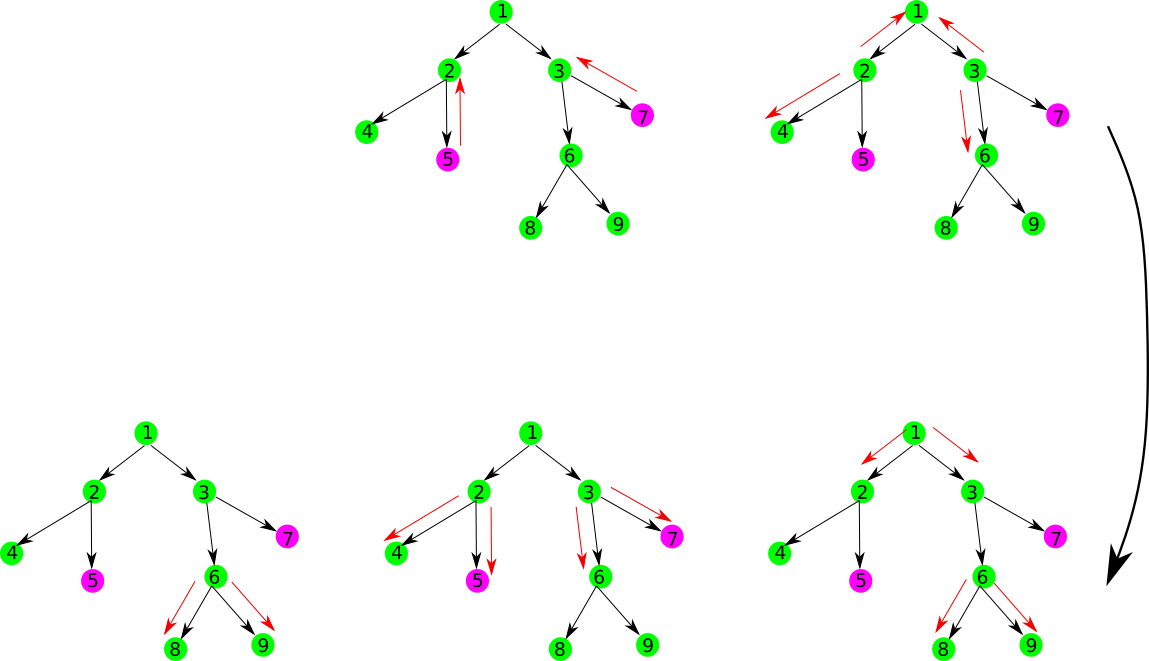
\includegraphics[width=7in]
{mpass/mp-multiframe-9tree.png}
\caption{Steps encoded in
the bnet 
Fig.\ref{fig-propagation-9tree}.
} 
\label{fig-multiframe-9tree}
\end{figure}

\clearpage
\newpage
\section{Bipartite bnets}

By a {\bf bipartite bnet}
we will mean a bnet
in which all nodes
are either root nodes (parentless)
or leaf nodes (childless).
BP
simplifies when dealing with
bipartite bnets. Next,
we will explain how
it simplifies. But
before doing so,
let
us define
tree bnets and
show how these
can be replaced by
equivalent bipartite bnets.


A {\bf tree bnet}
is a bnet for which all
nodes have exactly
one parent except
for the apex root
node which has none.
A tree bnet
is very much like
the filing system
in a computer.

One can map a tree
 bnet (the \qt{source})
into
an equivalent
bipartite bnet (the \qt{image}) as follows.
Replace
each arrow

\beq
\xymatrix{
\rvx\ar[rr]&&\rvy
}
\eeq
of the tree bnet by


\beq
\xymatrix{
\rvx\ar[r]
&
\ul{P_{\rvy|\rvx}}
&
\rvy\ar[l]
}\;.
\eeq
For example,
the tree bnet Fig.\ref{fig-part3-tree}
has the image
bipartite bnet given by
Fig.\ref{fig-part3-tree-junc-tree}.
The
bnet Fig.\ref{fig-part3-tree-bip-bnet}
is just
a different
way of drawing the bnet
Fig.\ref{fig-part3-tree-junc-tree}.

\begin{figure}[h!]
$$\xymatrix{
\rvA\ar[d]\ar[rrd]
\\
\rvA_0\ar[d]\ar[rd]&&\rvA_1
\\
\rvA_{00}&\rvA_{01}
}
$$
\caption{Example of a tree bnet.}
\label{fig-part3-tree}
\end{figure}


\begin{figure}[h!]
$$\xymatrix{
\rvA\ar[d]\ar[rrd]
\\
\ul{P_{\rvA_0|\rvA}}&&\ul{P_{\rvA_1|\rvA}}
\\
\rvA_0\ar[u]\ar[d]\ar[rd]&&\rvA_1\ar[u]
\\
\ul{P_{\rvA_{00}|\rvA_0}}&\ul{P_{\rvA_{01}|\rvA_0}}
\\
\rvA_{00}\ar[u]&\rvA_{01}\ar[u]
}
$$
\caption{Bipartite bnet
corresponding
to tree bnet Fig.\ref{fig-part3-tree}.}
\label{fig-part3-tree-junc-tree}
\end{figure}

\begin{figure}[h!]
\centering
$$\xymatrix{
\rvA\ar[dr]\ar[drr]
&\rvA_{0}\ar[d]\ar[drr]\ar[drrr]
&\rvA_{1}\ar[d]
&\rvA_{00}\ar[d]
&\rvA_{01}\ar[d]
\\
&\ul{P_{\rvA_{0}|\rvA}}
&\ul{P_{\rvA_{1}|\rvA}}
&\ul{P_{\rvA_{00}|\rvA_0}}
&\ul{P_{\rvA_{01}|\rvA_0}}
}$$
\caption{
Different
way of drawing
the bnet Fig.\ref{fig-part3-tree-junc-tree}.}
\label{fig-part3-tree-bip-bnet}
\end{figure}

The TPMs, printed in blue,
for the image bipartite bnet
Fig.\ref{fig-part3-tree-junc-tree},
are as follows. We express the
TPMs of the image bnet
in terms of the
TPMs of the source bnet
Fig.\ref{fig-part3-tree}. Let

\beq\color{blue}
P(P_{\rvy|\rvx}| x, y)=
P_{\rvy|\rvx}(y|x)
\delta(P_{\rvy|\rvx}, 1)
+
(1-P_{\rvy|\rvx}(y|x))
\delta(P_{\rvy|\rvx}, 0)
\eeq
for all the
leaf
nodes $\ul{P_{\rvy|\rvx}}\in \bool$ of the
image bipartite bnet.
Also, let

\beq\color{blue}
P_\rvy(y)= \text{arbitrary prior}
\;
\eeq
for all the root nodes 
$\rvy$ of the
image bipartite bnet
except when
$\rvy$ corresponds to
the root node $\rvA$
of the source tree bnet.
In that exceptional case,

\beq\color{blue}
P_\rvy(y)= P_\rvA(y)
\;.
\eeq


\section{BP for
bipartite bnets (BP-BB)}
For
a bipartite
bnet as defined above,
with
root nodes $\rvx_i$
and leaf nodes $\rvf_\alp$,
let


\beq
nb(i)=\{\alp: \rvf_\alpha\in
nb(\rvx_i)\}
\;,
\eeq

\beq
nb(\alpha)=\{i: \rvx_i\in
nb( \rvf_\alpha)\}
\;,
\eeq

\beq
m_{\alp\ldart i}
(x_i)
=
\pi_{\rvf_\alpha \ldart\rvx_i }
(x_i)
\;,
\eeq

\beq
m_{\alp\rdart i}
(x_i)
=
\lam_{\rvf_\alp\rdart \rvx_i}
(x_i)
\;,
\eeq


\begin{figure}[h!]
\centering
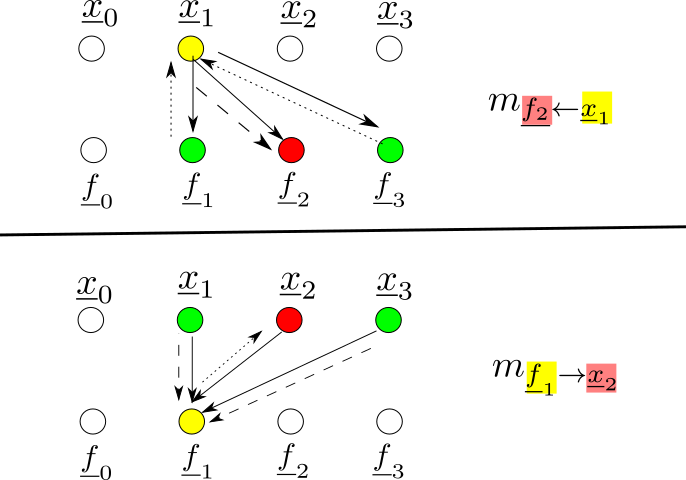
\includegraphics[width=3in]
{mpass/mpass-messages-bip.png}
\caption{
Fig.\ref{fig-messages-gen}
becomes this figure
for the special case of a
bipartite bnet. Union of green nodes and the red node = full
 neighborhood of yellow node.
There are two possible
cases:  the
red node is either a parent
or a child  of the yellow
node.}
\label{fig-messages-bip}
\end{figure}

Next we will
show how
to find $m_{\alp\ldart i}^{(t)}$
and $m_{\alp\rdart i}^{(t)}$
from 
$m_{\alp\ldart i}^{(t-1)}$
and $m_{\alp\rdart i}^{(t-1)}$.
\begin{enumerate}

\item {\bf
Traversing an $x$ (i.e., root) node.}

See
the
$m_{\rvf_2\ldart\rvx_2 }$ panel of
Fig.\ref{fig-messages-bip}.

For $i=0, 1, \ldots , nx-1$, if
 $\alp\in nb(i)$, then,

\beq
m^{(t)}_{\alp\ldart i }(x_i)
=
\prod_{
\beta\in nb(i)-\alpha}
m^{(t-1)}_{\beta\rdart i}(x_i)
\;,
\label{eq-mp-iter1}
\eeq
whereas if  $\alp\notin nb(i)$

\beq
m^{(t)}_{\alp\ldart i}(x_i)=
m^{(t-1)}_{\alp\ldart i}(x_i)
\;.
\eeq

\item {\bf
Traversing an $f$ (i.e., leaf) node.}

See the
$m_{\rvf_2\rdart \rvx_2}$ panel
of Fig.\ref{fig-messages-bip}.

For $\alp=0, 1, \ldots, nf-1$, if
 $i\in nb(\alp)$, then


\beqa
m^{(t)}_{\alp\rdart i}(x_i)
&=&
\sum_{(x_k)_{k\in nb(\alpha)-i}}
f_\alpha(x_{nb(\alpha)})
\prod_{k\in nb(\alpha)-i}
m^{(t-1)}_{\alp\ldart k }
(x_k)
\\
&=&
E^{(t-1)}_{(x_k)_{k\in nb(\alpha)-i}}[
f_\alpha(x_{nb(\alpha)})]
\;,
\label{eq-mp-iter2}
\eeqa
whereas if $i\notin nb(\alp)$

\beq
m^{(t)}_{\alp\rdart i}(x_i)
=
m^{(t-1)}_{\alp\rdart i}(x_i)
\;.
\eeq

\end{enumerate}

In the above
equations, if the
range set of a product is empty, then
 define the product as 1; i.e.,
$\prod_{k\in \emptyset}F(k)=1$.



\hrule\noindent
{\bf Claim:}

\beq
P(x_i|\eps)=
\lim_{t\rarrow
\infty}\caln(!x_i)\prod_{\alp\in nb(i)}
m^{(t)}_{\alp\rdart i}(x_i)
\;
\label{eq-m-prod}
\eeq
and

\beq
P(x_{nb(\alp)}|\eps)=\lim_{t\rarrow \infty}
\caln(!x_{nb(\alp)})
f_\alp(x_{nb(\alp)})
\prod_{k\in nb(\alp)}
m^{(t)}_{\alp\ldart k}(x_k)
\;.
\label{eq-f-m-prod}
\eeq


\subsection{BP-BB and general BP agree on Markov chains}

It is instructive to 
compare the belief values (i.e., $P(x_i|\eps)$)
obtained by
 applying the 
general (i.e., polytree)  BP  
and  BP-BB algorithms  to a Markov chain.
Next we show that both algorithms 
yield the same belief values.

\begin{figure}[h!]
$$
\begin{array}{cc}
\xymatrix{
&2\ar[dr]\ar[dl]\ar@[red]@{-->}@<-1ex>[dl]
\\
\beta
&&\alp\ar@[red]@{.>}@<-1ex>[ul]
}
&
\xymatrix{
&2\ar[dr]\ar[dl]\ar@[red]@{-->}@<1ex>[dr]
\\
\beta\ar@[red]@{.>}@<1ex>[ur]
&&\alp
}
\\
\\
(a)&(b)
\end{array}
$$
\caption{Traversing a root node of a Markov chain
(a)Propagation towards left (i.e., towards future).
(b)Propagation towards right (i.e., towards past).}
\label{fig-mp-markov-trans-root}
\end{figure}

Consider
the BP-BB rule for traversing a root node. 
When traveling
towards the left
as in Fig.\ref{fig-mp-markov-trans-root} (a), 
it implies that

\beq
m_{\alp \rdart 2}(x_2)= m_{\beta \ldart 2}(x_2)
\;,
\eeq
and
when traveling
towards the right
as in Fig.\ref{fig-mp-markov-trans-root} (b), 
it implies that

\beq
m_{\beta\rdart 2}(x_2)=m_{\alp\ldart 2}(x_2)
\;.
\eeq



\begin{figure}[h!]
$$
\begin{array}{cc}
\xymatrix{
3\ar[dr]
&&
2\ar[rd]\ar[dl]\ar@[red]@{-->}@<-1ex>[dl]
&&
1\ar[ld]\ar@[red]@{-->}@<1ex>[dl]
\\
&\beta
&&\alp\ar@[red]@{.>}@<-1ex>[ul]
}
&
\;\;\;\;\;
\xymatrix{
3\ar[dr]
&&
2\ar[rd]\ar[dl]\ar@[red]@{-->}@<1ex>[dr]
&&
1\ar[ld]
\\
&\beta\ar@[red]@{.>}@<1ex>[ur]
&&\alp\ar@[red]@{.>}@<-1ex>[ur]
}
\\
\\
(a)&(b)
\end{array}
$$
\caption{Traversing a leaf node of a Markov chain
(a)Propagation towards left (i.e., towards future).
(b)Propagation towards right (i.e., towards past).}
\label{fig-mp-markov-trans-leaf}
\end{figure}

Now consider the BP-BB rule for traversing a leaf node.
When
traveling to the left as
in Fig.\ref{fig-mp-markov-trans-leaf} (a),
it implies that

\beq
\underbrace{m_{\alp\rdart 2}(x_2)}_{\lam}
=
\sum_{x_1}
P(x_2|x_1) 
\underbrace{m_{\alp\ldart 1}(x_1)}_
{\pi}
\;.
\label{eq-markov-leaf-left}
\eeq
One can rewrite the
left and right
hand sides (LHS, RHS)
of Eq.(\ref{eq-markov-leaf-left})
as follows
 


\beq
RHS=
\sum_{x_1}
P(x_2|x_1) 
\pi_{\alp\ldart 1}(x_1)
\;,
\eeq
and

\beq
LHS=m_{\alp\rdart 2}(x_2)
=
m_{\beta\ldart 2}(x_2)
=
\pi_{\beta\ldart 2}(x_2)
\;,
\eeq
Therefore
 
\beq
\pi_{\beta\ldart 2}(x_2)
\sum_{x_1}
P(x_2|x_1) 
\pi_{\alp\ldart 1}(x_1)
\;.
\eeq


Once again, consider the BP-BB rule
 for traversing a leaf node.
When
traveling to the right as
in Fig.\ref{fig-mp-markov-trans-leaf} (b),
it implies that


\beq
\underbrace{m_{\alp\rdart1}(x_1)}_{\lam}
=
\sum_{x_2}
P(x_2|x_1) 
\underbrace{m_{\alp\ldart 2}(x_2)}_
{\pi}
\label{eq-markov-leaf-right}
\;.
\eeq
One can rewrite the
left and right
hand sides (LHS, RHS)
of Eq.(\ref{eq-markov-leaf-right})
as follows


\beqa
RHS=
&=&
\sum_{x_2}
P(x_2|x_1) 
\pi_{\alp\ldart 2}(x_2)
\\
&=&
\sum_{x_2}
P(x_2|x_1) 
\lam_{\beta\rdart 2}(x_2)
\;,
\eeqa
and

\beq
LHS=
\lam_{\alp\rdart 1}(x_1)
\;.
\eeq
Therefore,

\beq
\lam_{\alp\rdart 1}(x_1)=
\sum_{x_2}
P(x_2|x_1) 
\lam_{\beta\rdart 2}(x_2)
\;.
\eeq

Finally, note that Eq.(\ref{eq-m-prod}) becomes
\beqa
P(x_2|\eps)&=&
\caln(!x_2)
m_{\beta\rdart 2}(x_2)
m_{\alp\rdart 2}(x_2)
\\
&=&
\caln(!x_2)
m_{\alp\ldart 2}(x_2)
m_{\alp\rdart 2}(x_2)
\\
&=&
\caln(!x_2)
\pi_{\alp\ldart 2}(x_2)
\lam_{\alp\rdart 2}(x_2)
\\
&=&
\caln(!x_2)
P(x_2|\eps^-)
P(x_2|\eps^+)
\eeqa
and Eq.(\ref{eq-f-m-prod}) becomes

\beqa
P(x_2, x_1)
&=&
\caln(!x_2, !x_1)
P(x_2|x_1)
m_{\alp\ldart 1}(x_1)
m_{\alp\ldart 2}(x_2)
\\
&=&
\caln(!x_2, !x_1)
P(x_2|x_1)
\pi_{\alp\ldart 1}(x_1)
\pi_{\alp\ldart 2}(x_2)
\;.
\eeqa

\subsection{BP-BB and general BP 
agree on tree bnets.}

It is instructive to 
compare the belief values (i.e., $P(x_i|\eps)$)
obtained by
 applying the 
general (i.e., polytree)  BP  
and  BP-BB algorithms  to a tree bnet.
Next we show that both algorithms 
yield the same belief values.

\begin{figure}[h!]
\centering
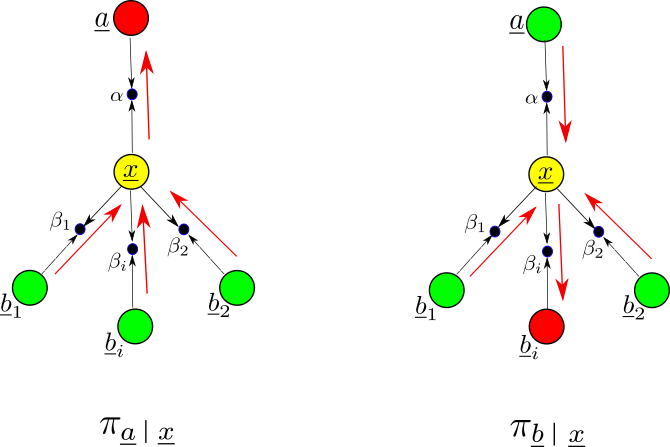
\includegraphics[width=4in]
{mpass/mpass-messages-bip-tree.png}
\caption{Subgraph of a tree bnet. 
This 
is the same as 
Fig.\ref{fig-messages-gen},
except that here the yellow
node has a single
parent because 
this is a subgraph of a tree
bnet, not
of an arbitrary
bnet like Fig.\ref{fig-messages-gen}.
The subgraph has been
converted to a subgraph
of a bipartite bnet
by inserting a collider leaf node, labeled
by a Greek letter, 
at the center
of each edge of the tree bnet.
Red arrows indicate
the direction
of message info flow.}
\label{fig-messages-bip-tree}
\end{figure}

Applying to the left panel of
Fig.\ref{fig-messages-bip-tree}
 the BP-BB rule
for traversing a root node, we get

\beq
m_{\alp\ldart \rvx}(x)=
\prod_{i}
m_{\beta_i\rdart \rvx}(x)
\;.
\label{eq-mp-tree-trans-x-rule1}
\eeq
Applying to the left panel of
Fig.\ref{fig-messages-bip-tree}
 the BP-BB rule
for traversing a leaf node, we get

\beq
m_{\alp\rdart\rva}(a)=
\caln(!a)
\sum_x
m_{\alp\ldart \rvx}(x)P(x|a)
\;.
\label{eq-mp-tree-trans-alp-rule1}
\eeq
Combining Eqs.(\ref{eq-mp-tree-trans-x-rule1})
and (\ref{eq-mp-tree-trans-alp-rule1}), we get

\beq
m_{\alp\rdart\rva}(a)=
\caln(!a)
\sum_x P(x|a)
\prod_{i}
m_{\beta_i\rdart \rvx}(x)
\;,
\eeq
which can be
rewritten as 

\beq
\lam_{\rvx\rdart\rva}(a)=
\caln(!a)
\sum_x P(x|a)
\underbrace{\prod_{i}
\lam_{\rvb_i\rdart \rvx}(x)}_
{\lam_\rvx(x)}
\;.
\label{eq-tree-rule1}
\eeq
Eq.(\ref{eq-tree-rule1}) is just RULE 1
for general BP.

Applying to the right panel of
Fig.\ref{fig-messages-bip-tree}
 the BP-BB rule
for traversing a root node, we get

\beq
m_{\beta_i\ldart \rvx}(x)=
\caln(!x)
m_{\alp\rdart \rvx}(x)
\prod_{k\neq i}m_{\beta_k\rdart\rvx}(x)
\label{eq-mp-tree-trans-x-rule2}
\eeq
Applying to the right panel of
Fig.\ref{fig-messages-bip-tree}
 the BP-BB rule
for traversing a leaf node, we get

\beqa
m_{\alp\rdart\rvx}(x)
&=&
\sum_a P(x|a) m_{\alp\ldart a}(a)
\\
&=&
\sum_a P(x|a) \pi_{\rvx\ldart a}(a)
\\
&=&
\pi_\rvx(x)
\label{eq-mp-tree-trans-alp-rule2}
\;.
\eeqa
Combining Eqs.(\ref{eq-mp-tree-trans-x-rule2})
and (\ref{eq-mp-tree-trans-alp-rule2}),
we get

\beq
\pi_{\rvb_i\ldart \rvx}(x)=
\caln(!x)
\pi_\rvx(x)
\prod_{k\neq i}\lam_{\rvb_k\rdart\rvx}(x)
\;.
\label{eq-tree-rule2}
\eeq
Eq.(\ref{eq-tree-rule2}) is just RULE 2
of general BP.




\section{BP-BB and sum-product decomposition}


BP-BB
yields what
is often
referred to as
a {\bf  sum-product decomposition}.
I don't like that name
because it is unnecessarily
confusing, and it fails to convey the
recursive nature\footnote{
By \qt{recursive nature},
we mean bootstrapped definitions 
that lead to nested sums. 
The recursive nature 
of BP
is evident from 
RULES 1 and 2
that define $\lam$'s 
and $\pi$'s
in terms of other 
$\lam$'s and $\pi$'s.}
of the decomposition.
I prefer to call it a {\bf
recursive sum of products
(RSOP) decomposition},
and will call it so henceforth
in this chapter.

Expressing the marginals of a bnet
as RSOPs,
which is what BP does,
reduces the complexity
of the calculation.
(i.e.,
the total number
of additions
and multiplications
that need to be performed)
That makes
using the BP
algo very advantageous.
For instance, consider 
a Markov chain
$\rvx_{n-1}\larrow\cdots\larrow\rvx_1\larrow \rvx_0$,
where $x_i\in\{0,1,2\}$ for all $i$.
Note that if we calculate 
$P(x_{n-1})$ as follows

\beq
P(x_{n-1})=
\left[\sum_{x_{n-2}} P(x_{n-1}|x_{n-2})\ldots
\left[\sum_{x_1} P(x_2|x_1)
\left[\sum_{x_0}P(x_1|x_0)P(x_0)\right]\right]\ldots\right]
\;,
\eeq
we need to perform 
 $2(n-1)$ additions and $3(n-1)$ multiplications.
On the other hand, if we calculate $P(x_{n-1})$
as follows 

\beq
P(x_{n-1})=
\sum_{x_{n-2}} \ldots
\sum_{x_1} 
\sum_{x_0}
P(x_{n-1}|x_{n-2})
\ldots
P(x_2|x_1)
P(x_1|x_0)
P(x_0)
\;,
\eeq
we need to perform $3^n-1$ additions and
 $3^n(n-1)$
multiplications.


\chapter{Monty Hall Problem}
\begin{figure}[h!]
\centering
$$\xymatrix{
\rvc\ar[dr]&&\rvy\ar[dl]\\
&\rvm&
}$$
\caption{Monty Hall Problem.}
\label{fig-monty}
\end{figure}

Mr. Monty Hall, host of the 
game show ``Let’s Make a Deal",
 hides a car behind one of 
three doors and a goat 
behind each of the other two.
 The contestant picks Door No. 1,
 but before opening it, Mr. Hall 
opens Door No. 2 to reveal a goat. 
Should the contestant stick with No. 1 
or 
switch to No. 3?

The Monty Hall problem can be 
modeled by the bnet 
Fig.\ref{fig-monty}, where
\begin{itemize}
\item
$\rvc$= the door behind which the car actually is.
\item
$\rvy$= the door opened by you
 (the contestant), on your 
first selection.
\item
$\rvm$= the door opened by Monty (game host)
\end{itemize}

We label the doors 1,2,3 so
 $S_\rvc=S_\rvy=S_\rvm=\{1,2,3\}$.

Node matrices printed in blue:
\beq\color{blue}
P(c)=\frac{1}{3}\text{ for all $c$}
\eeq

\beq\color{blue}
P(y)=\frac{1}{3}\text{ for all $y$}
\eeq

\beq\color{blue}
P(m|c,y)=\hat{1}(m\neq c)\left[
\frac{1}{2}\hat{1}(y=c)
+
\hat{1}(y\neq c)\hat{1}(m\neq y)\right]
\eeq

It's easy to show that the above
 node probabilities imply that
\beq
P(c=1|m=2,y=1)=\frac{1}{3}
\eeq

\beq
P(c=3|m=2,y=1)=\frac{2}{3}
\eeq

So you are twice as likely to
 win if you switch your final
 selection to be the door 
which is neither 
your first choice nor Monty’s choice.

The way I justify this to myself
is: Monty gives you a
 piece of information.
If you don't switch your choice,
you are wasting that info, whereas
if you switch, you are using the info.



\chapter{Naive Bayes}\label{ch-naive}

\begin{figure}[h!]
\centering
$$\xymatrix{
\rvc\ar[d]\ar[dr]\ar[drr]\ar[drrr]\\
\rvx_0&\rvx_1&\rvx_2&\rvx_3
}$$
\caption{bnet for Naive Bayes
with 4 features}
\label{fig-naive}
\end{figure}
Class node $\rvc\in S_\rvc$. $|S_\rvc|=n_\rvc$=
number of classes.

Feature nodes $\rvx_i\in S_{\rvx_i}$ for 
$i=0, 1, 2, \ldots, F-1$. $F$=number of
features.

Define
\beq
x.=[x_0,x_1, \ldots, x_{F-1}]
\;.
\eeq

For the bnet of Fig.\ref{fig-naive},
\beq
P(c, x.)=P(c)
\prod_{i=0}^{F-1}
P(x_i|c)
\;.
\eeq

Given $x.$ values, 
find most likely class $c\in S_\rvc$.

Maximum a Posteriori (MAP) estimate:
\beqa
c^* &=& \argmax_c P(c|x.)\\
&=&\argmax_c \frac{P(c,x.)}{P(x.)}\\
&=&\argmax_c P(c, x.)
\;.
\eeqa

\chapter{Neural Networks}

In this chapter, we discuss
 Neural Networks (NNs) of the
feedforward kind,
which is the most popular kind. In their
 plain, vanilla form, NNs only
have deterministic nodes.
But the nodes of a bnet can
be deterministic too, because
the transition probability matrix
of a node
can reduce to a delta function.
Hence, NNs should be expressible
as bnets. We will confirm this
in this chapter.

Henceforth in this chapter,
if we replace an index of an
indexed quantity by a dot, 
it will mean the collection
of the indexed quantity
for all values of that
index. For example, $x.$
will mean the 
array of $x_i$ for all $i$.


\begin{figure}[h!]
\centering
$$\xymatrix{
\rvx_0\ar@/^1pc/[rr]
\ar@/^2pc/[rrr]
\ar[d]\ar[dr]\ar[drr]\ar[r]&
\rvx_1\ar@/^1pc/[rr]
 \ar[dl]\ar[d]\ar[dr]\ar[r]&
\rvx_2\ar[dll]\ar[dl]\ar[d]\ar[r]&
\rvx_3\ar[dlll]\ar[dll]\ar[dl]\\
\rvh_0^0\ar[d]\ar[dr]&
\rvh_1^0\ar[dl]\ar[d]&
\rvh_2^0\ar[dll]\ar[dl]\\
\rvh_0^1\ar[d]\ar[dr]&
\rvh_1^1\ar[dl]\ar[d]\\
\rvY_0&
\rvY_1
}$$
\caption{Neural Network (feed forward)
with 4 layers: input layer $\rvx.$,
2 hidden layers $\rvh^0.$,
$\rvh^1.$ and
output layer $\rvY.$ }
\label{fig-nn}
\end{figure}

Consider Fig.\ref{fig-nn}.

$\rvx_i\in 
\{0,1\}$ for 
$i=0, 1, 2, \dots,numx-1$
is the \textbf{input layer}.

$\rvh_i^\lam\in \RR$ for 
$i=0, 1, 2, \dots,numh(\lam)-1$
is the $\lam$\textbf{-th hidden layer}.
$\lam=0, 1, 2, \ldots, \Lambda-1$.
A NN is said to be {\bf deep} if
$\Lambda>1$; i.e., if it has 
more than one hidden layer.

$\rvY_i\in \RR$ for 
$i=0, 1, 2, \dots,numy-1$
is the \textbf{output layer}.
We use a upper case y
here because in the training phase,
we will use pairs $(x.[s],y.[s])$ where
$y_i[s]\in \{0,1\}$ 
for $i=0, 1, \ldots, numy-1$.
$Y=\hat{y}$
is an estimate of $y$.
Note that lower case y is 
either 0 or 1, 
but upper case y may be 
any real. Often, the
activation
functions are chosen so that
$Y\in[0,1]$. 
 

The number of nodes in each layer 
and the number of layers are arbitrary.
Fig.\ref{fig-nn} is fully connected 
(aka dense), meaning that every node
of a layer is impinged 
arrow coming 
from every node of the preceding
layer. Later on in this chapter,
we will
discuss non-dense layers.

Let
  $w^\lam_{i|j}, b_i^\lam\in \RR$
be given,
for $i\in\ZZ_{[0, numh(\lam))}$,
$j\in\ZZ_{[0, numh(\lam-1))}$, 
and $\lam\in\ZZ_{[0, \Lambda)}$.

These are the
transition probability matrices,
printed in blue, for 
the nodes of the bnet 
Fig.\ref{fig-nn}:
 

\beq\color{blue}
P(x_i\cond x_{i-1},
x_{i-1},\dots, x_0)\text{ = given}
\eeq

\beq\color{blue}
P(h^{\lam}_i\cond h^{\lam-1}_.)=
\delta\left(h^{\lam}_i,
\cala_i^\lam(\sum_j w^{\lam-1}_{i|j}
h^{\lam-1}_j + b^{\lam-1}_i)\right)
\eeq

\beq\color{blue}
P(Y_i\cond h^{\Lambda-1}_.)=
\delta\left(Y_i,
\cala_i^\Lambda(\sum_j w^{\Lambda-1}_{i|j}
h^{\Lambda-1}_j + b^{\Lambda-1}_i)\right)
\eeq




\begin{center}
\LARGE\textbf{{Activation Functions} 
$\cala_i^\lam:\RR\rarrow \RR$}
\end{center}
Activation functions must be
nonlinear.

\begin{itemize}
\item {\bf Step function (Perceptron)}

\beq
\cala(x)=\indi(x>0)
\eeq
Zero for $x\leq 0$, one for $x>0$.

\item {\bf Sigmoid function}

\beq
\cala(x)=\frac{1}{1+e^{-x}}
\eeq
Smooth, monotonically increasing 
function.
$\cala(-\infty)=0$,$\cala(0)=0.5$,
$\cala(\infty)=1$

\item {\bf Hyperbolic tangent}
\beq
\cala(x)=\tanh(x)
\eeq
As with sigmoid: smooth,
 monotonically increasing function,
goes
from 0 to 1 as $x$ goes 
from $-\infty$ to
$\infty$.
\item {\bf ReLU (Rectified Linear Unit)}

For some $c>0$,
\beq
\cala(x)=cx\indi(x>0)
\;.
\eeq
Compare this to the step function.

\item {\bf Swish}
\beq
\cala(x)=x*sigmoid(x)
\eeq
\item {\bf Softmax}

\beq
\cala(x_i
|x.)=\frac{e^{x_i}}{\sum_i e^{x_i}}
\label{eq-softmax}
\eeq
It's called softmax because if we 
approximate the exponentials,
 both in the numerator and denominator
of Eq.(\ref{eq-softmax}),
by the largest one,
we get

\beq
\cala(x_i|x.)\approx \indi(x_i=\max_k x_k)
\;.
\eeq

The softmax definition implies
that the bnet nodes
 within a softmax layer
are fully connected by arrows
to form a ``clique".

\end{itemize}

\begin{center}
\LARGE\textbf{{Weight 
optimization via
supervised training and
gradient descent}}
\end{center}

The bnet of Fig.\ref{fig-nn}
is used for classification
of a single data point $x.$.
It assumes that the
weights $w^\lam_{i|j}, b_i^\lam$
are given.

To find the optimum
weights via supervised
training and gradient descent,
one uses the bnet Fig.\ref{fig-nn-ext}.

In Fig.\ref{fig-nn-ext},
the nodes in
Fig.\ref{fig-nn} become 
sampling space vectors.
For example, $\rvx.$ becomes
$\ranvec{x.}$, where the
components of 
$\ranvec{x.}$ in sampling space are
$\rvx.[s]\in \{0,1\}^{numx}$
for $s=0, 1, \ldots, nsam(\vecx)-1$.


$nsam(\vecx)$
is the number of
samples used to calculate the
gradient
during each {\bf stage (aka iteration)} of
Fig.\ref{fig-nn-ext}.
We will also  refer to
$nsam(\vecx)$ as the {\bf mini-batch size}.
A {\bf mini-batch} is a subset 
of the training data set.



To train a bnet with a data
set (d-set),
the standard procedure
is to split the d-set into 3 parts:
\begin{enumerate}
\item
{\bf training d-set}, 
\item
{\bf testing1 d-set}, for
tuning
of hyperparameters 
like $nsam(\vecx)$,  $\Lambda$,
and $nunh(i)$
for each $i$. 
\item
{\bf testing2 d-set}, for measuring
how well the model
tuned with the testing1 d-set
performs.
\end{enumerate}

The training d-set is 
itself split into mini-batches.
An {\bf epoch} is a pass through all 
the training d-set.

Define
\beq
W^\lam_{i|j}=[w^\lam_{i|j}, b^\lam_i]
\;.
\eeq

These are the
transition probability matrices,
printed in blue, for 
the nodes of the bnet 
Fig.\ref{fig-nn-ext}:

\begin{figure}[h!]
\centering
$$\xymatrix{
&&\ranvec{x.}\ar[d]\ar[r]&
\ranvec{y.}\ar[dddd]\\
&\rvW^0_{.|.}, \ar[r]&
\ranvec{h^0_.}\ar[d]\\
&\rvW^1_{.|.}\ar[r]&
\ranvec{h^1_.}\ar[d]\\
&\rvW^2_{.|.}\ar[r]&
\ranvec{h^2_.}\ar[d]\\
\rvW^._{.|.}\ar[ru]\ar[ruu]\ar[ruuu]
\ar@/_2pc/[rrrr]
&&
\vec{\rvY}.\ar[r]&\cale\ar[r]&
(\rvW')^._{.|.}
}$$
\caption{bnet 
for 
finding optimum
weights of the bnet 
Fig.\ref{fig-nn} via
supervised training
and gradient descent.
}
\label{fig-nn-ext}
\end{figure}

\beq\color{blue}
P(x.[s])
\text{ = given}
\;.
\eeq

\beq\color{blue}
P(y.[s]\cond x.[s])
\text{ = given}
\;.
\eeq

\beq\color{blue}
P(h^{\lam}_i[s]\cond h^{\lam-1}_.[s])=
\delta\left(h^{\lam}_i[s],
\cala_i^\lam(\sum_j w^{\lam-1}_{i|j}
h^{\lam-1}_j[s] + b^{\lam-1}_i)\right)
\eeq

\beq\color{blue}
P(Y_i[s]\cond h^{\Lambda-1}_.[s])=
\delta\left(Y_i[s],
\cala_i^\Lambda(\sum_j
 w^{\Lambda-1}_{i|j}
h^{\Lambda-1}_j[s] + b^{\Lambda-1}_i)\right)
\eeq

\beq\color{blue}
P(W^._{.|.})\text{ = given}
\eeq
The first time it is used,
 $W^._{.|.}$ is arbitrary.
After the first time, it is determined 
by previous stage.



\beq\color{blue}
P(W^\lam_{.|.}|W^._{.|.})
=
\delta(W^\lam_{.|.},
(W^._{.|.})^\lam)
\eeq

\beq\color{blue}
P(\cale|\vec{y}., \vec{Y}.)=
\frac{1}{nsam(\vecx)}
\sum_s\sum_i d(y_i[s], Y_i[s])
\;,
\eeq
where 

\beq
d(y,Y)=|y-Y|^2
\;.
\eeq
If $y, Y\in [0,1]$, 
one can use 

\beq
d(y,Y)=XE(y\rarrow Y)=
-y\log Y - (1-y)\log (1-Y)
\eeq
instead.

\beq\color{blue}
P((W')^\lam_{i|j}|\cale, W^._{.|.})
=
\delta((W')^\lam_{i|j},
W_{i|j}^\lam -\alpha
\partial_{W_{i|j}^\lam} \cale
)
\eeq
$\alpha>0$ is called the learning rate.
\begin{center}
\LARGE{\bf Non-dense layers}
\end{center}


The transition
probability matrix for
a non-dense layer is of the
form: 

\beq\color{blue}
P(h^\lam_i[s]\cond h^{\lam-1}_.[s])=
\delta(h^\lam_i[s],H^\lam_i[s])
\;,
\eeq
where
$H^\lam_i[s]$ will
be specified below for each type of
non-dense layer.

\begin{itemize}
\item{\bf Dropout Layer}

The dropout layer was
invented in Ref.\cite{dropout}.
To dropout nodes from a fixed 
layer $\lam$:
For all $i$ of layer $\lam$, 
define a new node $\rvr^\lam_i$
with an arrow 
$\rvr^\lam_i\rarrow\rvh^\lam_i$.
For $r\in \{0,1\}$, 
and some $p\in (0,1)$, define

\beq\color{blue}
P(r^\lam_i=r)=[p]^r
[1-p]^{1-r}
\text{ (Bernouilli dist.)}
\;.
\eeq
Now one has

\beq \color{blue}
P(h^\lam_i[s]\cond h^{\lam-1}_.[s], r^\lam_i)=
\delta(h^\lam_i[s],H^\lam_i[s])
\;,
\eeq
where

\beq
H^\lam_i[s]=
\cala^\lam_i(
r^\lam_i\sum_j w^\lam_{i|j}h^{\lam-1}_j[s]
+b^\lam_i
)
\;.
\eeq

This reduces ovefitting.
Overfitting might 
occur if the weights follow too closely
several similar minibatches.
This dropout procedure adds a random
component to each minibatch
making groups of similar minibatches
less likely.

The random $\rvr^\lam_i$ nodes
that induce dropout are 
only used in the training bnet Fig.\ref{fig-nn-ext},
not in the classification bnet Fig.\ref{fig-nn}.
We prefer to remove the 
$\rvr^\lam_i$ stochasticity from classification 
and for Fig.\ref{fig-nn} to act as an average
over sampling space of Fig.\ref{fig-nn-ext}.
Therefore,
if weights $w^\lam_{i|j}$ are obtained
for a dropout layer $\lam$ in Fig.\ref{fig-nn-ext},
then that layer is used in Fig.\ref{fig-nn} with 
no $\rvr^\lam_i$ nodes but
with weights $\av{r^\lam_i}w^\lam_{i|j}=
pw^\lam_{i|j}$.


Note that dropout adds non-deterministic
nodes to a NN, 
which in their vanilla form only have
deterministic nodes.


\item {\bf Convolutional Layer}

\begin{itemize}
\item 1-dim

Filter function $\calf:\{0, 1, \ldots, 
numf-1\}\rarrow \RR$.

$\sigma$=stride length

For $i\in \{0,1,\dots,numh(\lam)-1\}$,
let

\beq
H^\lam_i[s]=
\sum_{ j=0}^{numf-1}
h^{\lam-1}_{j+i\sigma}[s] \calf(j)
\;.
\label{eq-conv1}
\eeq
For the indices not to
go out of bounds in Eq.(\ref{eq-conv1}),
we must have

\beq
numh(\lam-1)-1=numf-1 +
(numh(\lam)-1)\sigma
\;
\eeq
so
\beq
numh(\lam)=\frac{1}{\sigma}[numh(\lam-1)-
numf] + 1
\;.
\eeq
\item 2-dim

$h_i^\lam[s]$ becomes
$h_{(i,j)}^\lam[s]$.
Do 1-dim convolution
along both $i$ and $j$ axes.

\end{itemize}
\item{\bf Pooling Layers 
(MaxPool, AvgPool)}

Here each node $i$ 
of layer $\lam$ is impinged by
arrows from  a subset $Pool(i)$
of the set of all
nodes of the previous layer $\lam-1$.
Partition set
$\{0,,1,\dots,numh(\lam-1)-1\}
$ into $numh(\lam)$ mutually
disjoint, nonempty sets
called $Pool(i)$, where
$i\in \{0, 1, \ldots,numh(\lam)-1\}$.

\begin{itemize}
\item AvgPool
\beq
H^\lam_i[s]=\frac{1}
{size(Pool(i))}
\sum_{j\in Pool(i)}h^{\lam-1}_j[s]
\eeq
\item MaxPool
\beq
H^\lam_i[s]=
\max_{j\in Pool(i)}h^{\lam-1}_j[s]
\eeq

\end{itemize}


\end{itemize}


\chapter{Noisy-OR gate}\label{ch-noisy-or}
The Noisy-OR gate was first
proposed by Judea Pearl in his 1988 book
 Ref.\cite{pearl-1988book}.
\begin{figure}[h!]
$$\xymatrix{
\rvx_0\ar@/_1pc/[ddrr]
&&\rvx_1\ar@/_1pc/[dd]
&&\rvx_2\ar@/_1pc/[ddll]
\\
&\ul{\pi}_0\ar[dr]
&\ul{\pi}_1\ar[d]
&\ul{\pi}_2\ar[dl]
\\
&\ul{\lam}\ar[r]
&\rvy
}$$
\caption{Noisy-OR gate $\rvy\in\bool$
with $n=3$, Boolean inputs $(\rvx_i)_{i=0,1,2}$
and parameters 
$\ul{\lam}, (\ul{\pi})_{i=0,1,2}$.
}
\label{fig-noisy-or-simple}
\end{figure}

Let

$\ul{\lam}\in [0, 1]=${\bf gate lea.k.a.ge}.

$y\in \bool$ = gate  output

$\rvx^n=(\rvx_i)_{i=0,1, \ldots, n-1}$, where
$\rvx_i\in\bool$ are
 gate inputs.

$\ul{\pi}^n=(\ul{\pi}_i)_{i=0,1, \ldots, n-1}$, where
$\ul{\pi}_i\in[0,1]$ are
 gate parameters.


The TPM, printed in blue,
 for the Noisy-OR gate $\rvy$ 
shown in Fig.\ref{fig-noisy-or-simple},
 is as follows.

\beq\color{blue}
P(y=1|x^n, \lam, \pi^n)=
1-(1-\lam)\prod_i[1-\pi_i x_i]
\label{eq-noisy-or-tmp-1}
\eeq
\beq\color{blue}
P(y=0|x^n, \lam, \pi^n)=
1-P(y=1|x^n, \lam, \pi^n)
\eeq

Note
that if $\lam=0$ and $\pi_i=1$ for all $i$,
then this becomes 
a deterministic OR-gate. Indeed,

\beq
P(y=1|x^n, \lam=0, \pi^n=1^n)= 1-\prod_i[1-x_i]=
\V_{i=0}^{n-1}x_i
\;,
\eeq
so 

\beq
P(y|x^n, \lam=0, \pi^n=1^n)=
\delta(y, \V_{i=0}^{n-1}x_i)
\;.
\eeq

\section{3 ways to interpret
the parameters $\pi_i$}
\begin{enumerate}
\item
Note that if $\lam=0$ and $x^n$ is one hot (i.e., 
$x^n=e^n_i$, where $e^n_i$
is the vector with all components 
zero except for the $i$-th
component which equals 1), then

\beq
P(y=1|x^n=e^n_i, \lam=0, \pi^n)=
1-[1-\pi_i]=\pi_i
\;.
\eeq
This gives an interpretation to the
parameters $\pi_i$.

\item

\begin{figure}[h!]
$$\xymatrix{
\rvh_0\ar[ddr]
&&\rvh_1\ar@/_1pc/[dd]
&&\rvh_2\ar[ddl]
\\
\rvx_0\ar[rd]
&&\rvx_1\ar[d]
&&\rvx_2\ar[ld]
\\
&\rvA_0\ar[dr]
&\rvA_1\ar[d]
&\rvA_2\ar[dl]
\\
&\ul{\lam}\ar[r]
&\rvy
}$$
\caption{Fig.\ref{fig-noisy-or-simple}
after replacing parameters 
$(\ul{\pi}_i)_{i=0,1,2}$
by 
hidden nodes
$(\rvh_i)_{i=0,1,2}$.}
\label{fig-noisy-or-hid}
\end{figure}


Another way of
interpreting the 
parameters $\pi_i$
is to associate 
each of them with a hidden 
variable
$\rvh_i\in \bool$
whose average equals $\pi_i$.
More precisely, 
consider Fig.\ref{fig-noisy-or-hid}.

Let $\rvx_i, \rvh_i, \rvA_i, \rvy\in \bool$.

The TPMs, printed  in blue, for the
bnet
Fig.\ref{fig-noisy-or-hid},
are as follows:

\beq\color{blue}
P(h_i)=\pi_i\delta(h_i,1)
+(1-\pi_i)\delta(h_i,0)
\eeq

\beq\color{blue}
P(A_i|h_i, x_i)= \delta(A_i, h_i\A x_i)
= \delta(A_i, h_i x_i)
\eeq

\beqa\color{blue}
P(y=1|A^n)&=& 
\color{blue}
1-(1-\lam)
 \A_{i=0}^{n-1}
\ol{A}_i
\\
&=&
\color{blue}
 1 - (1-\lam) \prod_i(1-A_i)
\eeqa

\beq\color{blue}
P(y=0|A^n)=1-P(y=1|A^n)
\eeq


Note that

\begin{align}
P(y=1|x^n, \lam)
&=
\sum_{h^n}
\sum_{A^n}
\left[
 1 - (1-\lam) 
\prod_i(1-A_i)\right]
[\prod_i \delta(A_i, h_i x_i)]P(h^n)
\\
&=
E_{\rvh^n}\left[
[ 1 - (1-\lam) \prod_i(1-h_i x_i)
\right]
\;.
\end{align}
But


\beq
E_{\rvh_i}[h_i x_i]=
\sum_{h_i=0,1} P(h_i)h_i x_i
=
\pi_i x_i
\eeq
so


\beq
P(y=1|x^n, \lam)=
1 - (1-\lam) \prod_i(1-\pi_i x_i)
\;.
\eeq



\item

\begin{figure}[h!]
$$\xymatrix{
\ul{\vech}_0\ar[ddr]
&&\ul{\vech}_1\ar@/_1pc/[dd]
&&\ul{\vech}_2\ar[ddl]
\\
\rvx_0\ar[rd]
&&\rvx_1\ar[d]
&&\rvx_2\ar[ld]
\\
&\rvA_0\ar[dr]
&\rvA_1\ar[d]
&\rvA_2\ar[dl]
\\
&\ul{\lam}\ar[r]
&\rvy
}$$
\caption{ Fig.\ref{fig-noisy-or-hid}
after replacing the hidden nodes 
$(\rvh_i)_{i=0,1,2}$
by 
vectors 
of samples $(\vec{\rvh}_i)_{i=0,1,2}$.}
\label{fig-noisy-or-sams}
\end{figure}

Another way to
interpret the 
parameters $\pi_i$
is to associate each of 
them with a vector of samples
$\vec{\rvh}_i$
whose average is $\pi_i$.
More precisely,
consider Fig.\ref{fig-noisy-or-sams}.

Suppose  $\rvh_i\in \bool$ and
define

\beq
P_{\rvh_i}(h_i)=
\pi_i\delta(h_i, 1)
+
(1-\pi_i)\delta(h_i, 0)
\;.
\eeq
Suppose $\vec{\rvh}_i=(\rvh_i[\sigma])_
{s=0, 1, \ldots, nsam-1}$ 
and  the 
Boolean samples $\rvh_i[\sigma]\in \bool$
 are i.i.d. with
$\rvh_i[\sigma]\sim P_{\rvh_i}$
for all $\sigma$.

Note that for each $i$,
an estimate 
$\HAT{P}_{\rvh_i}(h_i)$
of
$P_{\rvh_i}(h_i)$
can be 
obtained
from the vector of samples
$\vec{\rvh}_i$ 
as follows:


\beq
\HAT{P}_{\rvh_i}(h_i)=
\frac{1}{nsam}
\sum_{\sigma=0}^{nsam-1} \indi(h_i[\sigma]=h_i)
\;.
\eeq


Let $\rvx_i, \rvh_i[\sigma], \rvA_i, \rvy\in \bool$.

The TPMs, printed  in blue, for the
bnet
Fig.\ref{fig-noisy-or-sams},
are as follows:

\beq\color{blue}
P(\vech_i)=\prod_{\sigma=0}^{nsam-1}
P_\rvh(h_i[\sigma])
\eeq

\beqa\color{blue}
P(A_i\cond \vech_i, x_i)
&=&\color{blue}
\delta(A_i, \frac{1}{nsam}\sum_\sigma
 h_i[\sigma]\A x_i)
\\
&=&\color{blue}
\delta(A_i, 
 \pi_i x_i)
\eeqa

\beqa\color{blue}
P(y=1|A^n)&=& 
\color{blue}
1-(1-\lam)
 \A_{i=0}^{n-1}
\ol{A}_i
\\
&=&
\color{blue}
 1 - (1-\lam) \prod_i(1-A_i)
\eeqa

\beq\color{blue}
P(y=0|A^n)=1-P(y=1|A^n)
\eeq



Note that

\begin{align}
P(y=1|x^n, \lam, \vech^n)
&=
\sum_{A^n}
\left[
 1 - (1-\lam) \prod_i
(1-A_i)\right]\prod_i
\delta(A_i, \pi_i x_i)
\\
&=
1 - (1-\lam) \prod_i(1-\pi_i x_i)
\;.
\end{align}


\end{enumerate}
\chapter{Non-negative Matrix Factorization}

Based on Ref.\cite{wiki-nmf}.

Given
 matrix $V$, factor it
 into product of two matrices

\beq
V=WH
\;,
\eeq 

where all 3 matrices
have non-negative entries.

$V\in \RR^{nv\times na}_{\geq 0}$: visible info matrix

$W\in \RR^{nv\times nh}_{\geq 0}$: weight info matrix

$H\in \RR^{nh\times na}_{\geq 0}$: hidden info matrix


Usually, $nv > nh<na$ so compression of
information (aka dimensional reduction,
 clustering)

\section{Bnet 
interpretation}

 Express node $\rvv$ as a chain of 
 two nodes.

\begin{figure}[h!]
\centering
$$\xymatrix{
\rvv& \rva\ar[l]&= &\rvw &\rvh\ar[l]&\rva\ar[l]
}$$
\caption{B net interpretation of 
non-negative matrix factorization.}
\label{fig-nmf}
\end{figure}
Node TPMs, printed in blue,
for Fig.\ref{fig-nmf}.

\beq\color{blue}
P(\rvv=w|a)=\frac{V_{w,a}}{\sum_w V_{w,a}}
\eeq

\beq\color{blue}
P(w|h)=\frac{W_{w,h}}{\sum_w W_{w,h}}
\eeq

\beq\color{blue}
P(h|a)=\frac{\sum_w W_{w,h}}{ \sum_w V_{w,a}}H_{h,a}
\eeq

\section{Simplest recursive
 algorithm}

Initialize: Choose $nh$. Choose $W^{(0)}$ and $H^{(0)}$
that have non-negative entries. 

Update: For $n=0, 1 , \dots $,
do

\beq
H_{i,j}^{(n+1)}\leftarrow H_{i,j}^{(n)}
\frac{
[(W^{(n)})^T V]_{i,j}
}{
[(W^{(n)})^T 
\underbrace{W^{(n)} H^{(n)}}_{\approx V}
]_{i,j}
}
\eeq
and
\beq
W_{i,j}^{(n+1)}\leftarrow W_{i,j}^{(n)}
\frac{
[V(H^{(n+1)})^T]_{i,j}
}
{
[
\underbrace{W^{(n)} H^{(n+1)}}_{\approx V}
(H^{(n+1)})^T]_{i,j}
}\;.
\eeq
After each step, record error defined by

\beq
\cale^{(n)} =\parallel V-W^{(n)}
H^{(n)}\parallel_2
\;.
\eeq
Using 2-norm, aka Frobenius matrix norm.
Continue until reach acceptable error.

Can also use Kullback-Lieber divergence for error:

\beq
\cale = 
\sum_a P(a)
 D_{KL}(P(\rvv=w|a)\parallel \sum_hP(w|h)P(h|a))
\;,
\eeq
for some arbitrary choice of prior $P(a)$. For 
example, can choose $P(a)$ uniform.
\chapter{Observational
 Equivalence of DAGs}\label{ch-obs-equi}

This chapter is based on Chapter 1 of
Ref.\cite{pearl-2013book}
and on a blog post by 
Bruno Gon\c{c}alves 
(Ref.\cite{bruno-obs-equiv}).



Two DAGs are {\bf observationally
equivalent (OE)}
if they
represent
the same
probability distribution.
For example,
$\rva\rarrow\rvb$
and $\rva\larrow\rvb$
are OE because

\beq
P(a|b)P(b)=P(a,b)=P(b|a)P(a)
\label{eq-two-node-prob}
\;.
\eeq

The {\bf
skeleton}
of a DAG is its
undelying undirected graph.

A {\bf v-structure}
in
a DAG consists of
two arrows 
converging to
a node and
such 
that their tails
are not 
connected 
by a third arrow.
Fig.\ref{fig-v-strucs}
shows in red all the v-structures 
of a particular DAG.

\begin{figure}[h!]
$$\xymatrix{
\rvz_1\ar[dd]\ar[rd]
&&\rvz_2\ar@[red][dd]\ar[ld]
\\
&\rvz_3\ar[dl]\ar[dr]
\\
\rvx\ar[r]&\rvw\ar@[red][r]&\rvy
\\
&(a)
}
\xymatrix{
\rvz_1\ar[dd]\ar@[red][rd]
&&\rvz_2\ar[dd]\ar@[red][ld]
\\
&\rvz_3\ar[dl]\ar[dr]
\\
\rvx\ar[r]&\rvw\ar[r]&\rvy
\\
&(b)
}
\xymatrix{
\rvz_1\ar[dd]\ar[rd]
&&\rvz_2\ar[dd]\ar[ld]
\\
&\rvz_3\ar[dl]\ar@[red][dr]
\\
\rvx\ar[r]&\rvw\ar@[red][r]&\rvy
\\
&(c)
}$$
\caption{Example showing in red
all v-structures 
of a particular DAG.}
\label{fig-v-strucs}
\end{figure}





\begin{claim}Observational Equivalence
Theorem (by Verma and Pearl, 1990)

Two DAGs are
OE
iff they
have the same
skeletons and
the same v-structures.
\end{claim}

\hrule\noindent {\bf Example}

\begin{figure}[h!]
$$\xymatrix{
&\rvx_1
\ar[dl]
\ar[dr]
\\
\rvx_2\ar[dr]
&&\rvx_3\ar[dl]
\\
&\rvx_4\ar[d]
\\
&\rvx_5
\\
&(a)
}
\;\;\;\;\;
\xymatrix{
&\rvx_1
\ar[dr]
\\
\rvx_2\ar[dr]\ar[ur]
&&\rvx_3\ar[dl]
\\
&\rvx_4\ar[d]
\\
&\rvx_5
\\
&(b)
}
\;\;\;\;\;
\xymatrix{
&\rvx_1
\ar[dl]
\\
\rvx_2\ar[dr]
&&\rvx_3\ar[dl]\ar[ul]
\\
&\rvx_4\ar[d]
\\
&\rvx_5
\\
&(c)
}$$
\caption{These 3 DAGs are 
observational equivalent (OE).}
\label{fig-obs-equi-eg}
\end{figure}
\begin{figure}[h!]
$$
\xymatrix{
&\rvx_1
\ar@{-}[dl]\ar@{-}[dr]
\\
\rvx_2\ar[dr]
&&\rvx_3\ar[dl]
\\
&\rvx_4\ar[d]
\\
&\rvx_5
\\
&(c)
}$$
\caption{This partially
directed graph 
represents the 3 
DAGs
in Fig.\ref{fig-obs-equi-eg}.}
\label{fig-pdag1}
\end{figure}

The 3 DAGs
in Fig.\ref{fig-obs-equi-eg}
are OE. They form an equivalence
class of OE DAGs
that represent
the same probability distribution.
This
equivalence
class of DAGs
can be represented
by the partially 
directed graph 
Fig.\ref{fig-pdag1}.
These 3 DAGs 
can be proven to 
be OE
in the following 3 ways:


\begin{enumerate}
\item
Write
the generic
probability
distributions
represented by
the 3 DAGs,
and show
that they are equal, as we did 
in Eq.\ref{eq-two-node-prob}.
That is the low brow way
of proving OE.
\item
Use d-separation
(see Chapter \ref{chap-dsep}).
Consider DAG $(a)$ first.
Rename the nodes as $\ul{\tau}_j$
with $j=1, 2, \ldots$
so that the names
are in topological
order (i.e., so that 
the parents of $\ul{\tau}_j$
have
indices that 
are smaller than $j$).
The node names $\rvx_j$
of DAG $(a)$
are already in topologigal
order, so we skip this step
for DAG $(a)$.
Now write down 
its total probability
distribution
and notice
which parents
of a fully connected DAG
were omitted.

\beq
P(x_1, x_2, x_3, x_4, x_5)
=
\underbrace{P(x_5|x_4)}
_{x_3, x_2, x_1 \text{ omitted}}
\underbrace{P(x_4|x_3, x_2)}
_{x_1\text{ omitted}}
\underbrace{P(x_3|x_1)}
_{x_2\text{ omitted}}
P(x_2|x_1)P(x_1)
\eeq
The
observations
of which parents
 were omitted
can be stated in d-separation lingo as
the following 3 orthogonality
relations:\footnote{
Normally,
if we had changed
from the 
original
node names to
the  
$\ul{\tau}_j$ node
names, 
these
orthogonality
relations
would first
be stated 
in terms
of the 
$\ul{\tau}_j$
names, 
and we 
could 
translate
them
so
that
they
were
stated 
in terms
of the 
original
node 
names.
But
for DAG
$(a)$
there was no need
to
use 
the $\ul{\tau}_j$ names.
}

\begin{subequations}
\label{eq-oe-ortho}
\beqa
\rvx_3 \perp_P \rvx_2 &|& \rvx_1
\\
\rvx_4 \perp_P \rvx_1 &|& \rvx_2, \rvx_3
\\
\rvx_5 \perp_P (\rvx_1, \rvx_2, \rvx_3) &|& \rvx_4
\;.
\eeqa
\end{subequations}



Going through the
same procedure
for the other 2 DAGs yields,
for each of them,
an equivalent set of 3 
orthogonality equations.\footnote{
The
$\rvx_j$
node
names
are 
no longer
in topological
order
for DAGs $(b)$
and $(c)$
so
for them
you
should
go through
the
intermediate step
of renaming the
nodes $\ul{\tau}_j$,
and 
then,
after
obtaining
the orthogonality
relations
in terms
of the
$\ul{\tau}_j$ names, 
translating
them
back to 
the original
$\rvx_j$ names.}

This is enough to
conclude that the 3 DAGs 
of Fig.\ref{fig-obs-equi-eg}
are OE.

Note that Eqs.(\ref{eq-oe-ortho})
encompass all that
there is to say about the
observability
of DAG $(a)$. These
3 equations
can be checked empirically
to assess how well the DAG fits
the data.
For example,
one can do
OLS (ordinary least squares) regression
$x_5\sim x_1+ x_2 + x_3 + x_4$ 
on the data, i.e., try 
to fit $x_5=
\beta_0 +
\sum_{i=1}^{4}\beta_i x_i$
to the data, and find that,
to a good approximation, 
$\beta_1=\beta_2=\beta_3=0$.




\item
Use the OE Theorem. All three
DAGs have the same
skeleton,
and the same
single
v-structure
$\rvx_2\rarrow\rvx_4\larrow\rvx_3$.




\end{enumerate}


\chapter{Program evaluation
 and review technique (PERT): COMING SOON}
\chapter{Recurrent Neural Networks}

This chapter is mostly
based on Ref.\cite{ng-rnn}.

This chapter
assumes you are
familiar 
with the material
and notation of Chapter \ref{ch-nn}
on plain Neural Nets.


\begin{figure}[h!]
\centering
$$\xymatrix{
\rvx(0)\ar[d]&
\rvx(1)\ar[d]&
\rvx(2)\ar[d]\\
\rvh(0)\ar[d]\ar[r]&
\rvh(1)\ar[d]\ar[r]&
\rvh(2)\ar[d]\\
\rvY(0)&
\rvY(1)&
\rvY(2)
}$$
\caption{Simple example of 
RNN witb $T=3$}
\label{fig-rnn}
\end{figure}

Suppose

$T$ is a positive integer.

$t=0, 1, \ldots, T-1$,

$\rvx_i(t)\in \RR$ for
 $i=0,1, \ldots,numx-1$,

$\rvh_i(t)\in \RR$ for
 $i=0,1, \ldots,numh-1$,

$\rvY_i(t)\in \RR$ for
 $i=0,1, \ldots,numy-1$,

$W^{h|x}\in\RR^{numh\times numx}$,

$W^{h|h}\in\RR^{numh\times numh}$,

$W^{y|h}\in\RR^{numy\times numh}$,

$b^y\in \RR^{numy}$,

$b^h\in \RR^{numh}$.

The simplest kind of
recurrent neural network (RNN)
has
the bnet Fig.\ref{fig-rnn}
with arbitrary $T$.
The node
transition matrices, printed in
blue, for this bnet, are as follows.

\beq\color{blue}
P(x(t))\text{ = given}
\eeq

\beq\color{blue}
P(h(t)\cond h(t-1), x(t))=
\delta(h(t),
\cala(W^{h|x}x(t) +
 W^{h|h}h(t-1) + b^h))
\;,
\eeq
where
$h(-1)=0$.

\beq\color{blue}
P(Y(t)\cond h(t))=
\delta(h(t),
\cala(W^{y|h}h(t) + b^y))
\eeq

Define

\beq
W^h=[W^{h|x}, W^{h|h}, b^h]
\;,
\eeq
and

\beq
W^y=[W^{y|h}, b^y]
\;.
\eeq

The bnet of Fig.\ref{fig-rnn}
can be used for
classification once 
its parameters 
$W^h$ and $W^y$
have been optimized.
To optimize
those parameters via gradient
descent,
one can use the bnet 
of Fig.\ref{fig-rnn-ext}.

Let $s=0,1, \ldots, nsam(\vecx)-1$
be the labels for a minibatch of samples.
The node transition matrices,
 printed in blue,
for bnet Fig.\ref{fig-rnn-ext},
 are as follows.



\begin{figure}[h!]
\centering
$$\xymatrix{
&\vec{\rvx}(0)\ar[d]\ar@/^1pc/[ddd]&
\vec{\rvx}(1)\ar[d]&
\vec{\rvx}(2)\ar[d]\\
\rvW^h\ar[r]\ar@/^2pc/[rr]\ar@/^2pc/[rrr]
\ar@/_3pc/[ddddd]
&\vec{\rvh}(0)\ar[d]\ar[r]&
\vec{\rvh}(1)\ar[d]\ar[r]&
\vec{\rvh}(2)\ar[d]\\
\rvW^y\ar[r]\ar@/^2pc/[rr]\ar@/^2pc/[rrr]
\ar@/_3pc/[ddddd]
&\vec{\rvY}(0)\ar@/^1pc/[dd]&
\vec{\rvY}(1)\ar@/^1pc/[dd]&
\vec{\rvY}(2)\ar@/^1pc/[dd]
\\
&
\vec{\rvy}(0)\ar[d]&
\vec{\rvy}(1)\ar[d]&
\vec{\rvy}(2)\ar[d]
\\
\ul{\cale}\ar[dd]
\ar@/_2pc/[ddd]&
\ul{\cale}(0)\ar[l]&
\ul{\cale}(1)\ar@/_1pc/[ll]&
\ul{\cale}(2)\ar@/_2pc/[lll]
\\
&
\vec{\rvx}(0)'
&\vec{\rvx}(1)'
&\vec{\rvx}(2)'
\\
(\rvW^h)'\\
(\rvW^y)'
}
$$
\caption{RNN bnet used
to optimze parameters $W^h$
and $W^y$ of RNN bnet Fig.\ref{fig-rnn}.}
\label{fig-rnn-ext}
\end{figure}

\beq\color{blue}
P(x(t)[s])\text{ = given}
\eeq

\beq\color{blue}
P(h(t)[s]\cond h(t-1)[s], x(t)[s])=
\delta(h(t)[s],
\cala(W^{h|x}x(t)[s] + W^{h|h}h(t-1)[s] + b^h)
\eeq

\beq\color{blue}
P(Y(t)[s]\cond h(t-1)[s])=
\delta(Y(t)[s],
\cala(W^{y|h}h(t-1)[s] + b^y)
\eeq

\beq\color{blue}
P(y(t)[s]\cond x(t)[s])\text{ = given}
\eeq

\beq\color{blue}
P(\cale(t)\cond \vecy(t), \vec{Y}(t))
=\frac{1}{nsam(\vecx)}
\sum_s d(y(t)[s], Y(t)[s])
\;,
\eeq
where 

\beq
d(y,Y)=|y-Y|^2
\;.
\eeq
If $y, Y\in [0,1]$, 
one can use 

\beq
d(y,Y)=XE(y\rarrow Y)=
-y\log Y - (1-y)\log (1-Y)
\eeq
instead.

\beq\color{blue}
P(\cale\cond [\cale(t)]_{\forall t})=
\delta(\cale, \sum_t \cale(t))
\eeq

For $a=h,y$,
\beq\color{blue}
P(W^a)\text{ = given}
\;.
\eeq
The first time it is used,
$W^a$ is fairly arbitrary. Afterwards,
it is determined by previous 
horizontal
stage.

\beq\color{blue}
P((W^a)'|\cale, W^a)=
\delta((W^a)', W^a -
\eta ^a\partial_{W^a}\cale)
\;.
\eeq
$\eta ^a>0$ is the learning rate
for $W^a$.

\section*{Language Sequence Modeling}

Figs.\ref{fig-rnn}, and \ref{fig-rnn-ext}
with arbirary $T$ can be used 
as follows to do
Language Sequence Modeling.

For this usecase, one must
train with the following
transition matrix for node $\vecy(t)$:

\beq\color{blue}
P(y(t)[s]\cond [x(t)[s]]_{t'\leq t})=
\indi(\;\;\;y(t)[s]=
P(x(t)[s]\cond [x(t')[s]]_{t'<t})
\;\;\;)
\eeq

With such training, one gets

\beq
P(Y(t)|h(t))=
\indi(\;\;\;
Y(t)=P(x(t)\cond [x(t')]_{t'<t})\;\;\;)
\;.
\eeq
Therefore,

\beq
Y(0)=P(x(0))
\;,
\eeq

\beq
Y(1)=P(x(1)|x(0))
\;,
\eeq

\beq
Y(2)=P(x(2)|x(0), x(1))
\;,
\eeq
and so on.

We can use this to: 
\begin{itemize}
\item
predict the probability 
of a sentence,

example: Get $P(x(0), x(1), x(2))$.
\item
predict 
the most likely 
next word in a sentence,

example: Get $P(x(2)| x(0), x(1))$.
\item generate fake sentences.

example: 

Get $x(0)\sim P(x(0))$.

Next get $x(1)\sim P(x(1)|x(0))$.

Next get $x(2)\sim P(x(2)|x(0), x(1))$.


\end{itemize}

 
\section*{Other types of RNN}

\begin{figure}[h!]
\centering
$$\xymatrix{
\rvx(0)\ar[d]&
\rvx(1)\ar[d]&
\\
\rvh(0)\ar[r]&
\rvh(1)\ar[r]&
\rvh(2)\ar[d]\ar[r]&
\rvh(3)\ar[d]\\
&
&
\rvY(2)&
\rvY(3)
}$$
\caption{RNN bnet of the
many to many kind. This
one can be used for  translation.
$x(0)$ and $x(1)$ might
denote two words of an English
sentence, and $Y(2)$ 
and $Y(3)$ might be
their Italian translation.}
\label{fig-rnn-translation}
\end{figure}

Let $\calt=\{0,1, \dots , T-1\}$,
and
$\calt^x, \calt^y\subset \calt$.
Above, 
we assumed that 
$\rvx(t)$ and $\rvY(t)$
were both defined 
for all $t\in \calt$.
More generally, they 
might be defined only
for subsets of $\calt$:
$\rvx(t)$ for $t\in \calt^x$
and 
$\rvY(t)$ for $t\in \calt^y$.
If $|\calt^x|=1$ and
$|\calt^y|>1$, 
we say the RNN bnet is of
the 1 to many kind.
In general, can have 
{\bf 1 to 1, 1 to many, many to 1, 
many to many} RNN bnets.

Plain RNNs can suffer 
from the
{\bf vanishing or exploding
 gradients problem}.
There are various ways to
mitigate this (good choice of initial
$W^h$ and $W^y$, 
good choice of activation 
functions, regularization).
Or by using GRU or LSTM (discussed below).
 {\bf GRU and LSTM}
were designed to mitigate
vanishing or exploding gradients problem.
They are very popular in NLP (Natural
Language Processing).



\newpage

\section*{Long  
Short Term Memory (LSTM) unit (1997)}

This section
is based on Wikipedia article 
Ref.\cite{lstm}. In this section,
$\odot$
will denote the Hadamard matrix product
(elementwise product)  
and $\sigma$ the sigmoid function.

\begin{figure}[h!]
\centering
$$\xymatrix{
&&\rvx(t)\ar[ddd]\ar[dl]\ar[ldd]\ar[lddd]
\\
&\rvi(t)\ar[rddd]
&\\
&\rvf(t)\ar[rdd]&\\
&\rvo(t)\ar[ddr]
&\tilde{\rvc}(t)\ar[d]
\\
\rvc(t-1)\ar[rr]
&&\rvc(t)\ar[d]
\\
\rvh(t-1)\ar[ruuuu]\ar[ruuu]\ar[ruu]\ar[rruu]
&&\rvh(t)\ar[d]\\
&&\rvY(t)
}$$
\caption{
bnet for a Long Short Term Memory
 (LSTM) unit.}
\label{fig-rnn-lstm}
\end{figure}

Let

$\rvx_{t}\in \RR^{numx}$: 
input vector to the LSTM unit

$\rvf_{t}\in \RR^{numh}$:
forget gate's activation vector

$\rvi_{t}\in \RR^{numh}$: 
input/update gate's activation vector

$\rvo_{t}\in \RR^{numh}$: 
output gate's activation vector

$\rvh_{t}\in \RR^{numh}$: 
hidden state vector also known as
 output vector of the LSTM unit

${\tilde {\rvc}}_{t}\in \RR^{numh}$: 
cell input activation vector

$\rvc_{t}\in \RR^{numh}$: 
cell state vector

$\rvY(t)\in \RR^{numy}$: 
classification of $x(t)$.

$W\in \RR^{numh\times numx}$, 
$U\in \RR^{numh\times numh}$
and 
$b\in \RR^{numh}$: 
weight matrices and bias vectors,
 parameters learned by training.

$\calw^{y|h}\in \RR^{numy\times numh}$:
 weight matrix


Fig.\ref{fig-rnn-lstm}
is a bnet net
for a LSTM unit.
The node transition matrices, printed in blue,
for this bnet, are
as follows.

\beq\color{blue}
P(f(t)|x(t), h(t-1))=\indi(\;\;\;
f(t)=\sigma(W^{f|x}x(t)+
U^{f|h}h(t-1)+b^{f})
\;\;\;)
\;,
\eeq
where $h(-1)=0$.

\beq\color{blue}
P(i(t)|x(t), h(t-1))=\indi(\;\;\;
i(t)=\sigma(W^{i|x}x(t)
+U^{i|h}h(t-1)+b^{i})
\;\;\;)
\eeq

\beq\color{blue}
P(o(t)|x(t), h(t-1))=\indi(\;\;\;
o(t)=\sigma(W^{o|x}x(t)
+U^{o|h}h(t-1)+b^{o})
\;\;\;)
\eeq

\beq\color{blue}
P(\tilde{c}(t)|x(t), h(t-1))=\indi(\;\;\;
\tilde{c}(t)=\tanh
(W^{c|x}x(t)+U^{c|h}h(t-1)+b^{c})
\;\;\;)
\eeq

\beq\color{blue}
P(c(t)|f(t), c(t-1), i(t),
 \tilde{c}(t))
=\indi(\;\;\;
c(t)=f(t)\odot c(t-1)+
i(t)\odot {\tilde {c}}(t)
\;\;\;)
\eeq

\beq\color{blue}
P(h(t)|o(t), c(t))=\indi(\;\;\;
h(t)=o(t)\odot \tanh
(c(t))
\;\;\;)
\eeq



\beq\color{blue}
P(Y(t)|h(t))=\indi(\;\;\;
Y(t)= \cala(\calw^{y|h}h(t) + b^y)
\;\;\;)
\eeq

\newpage
\section*{Gated Recurrence Unit
 (GRU) (2014)}

This 
section is based 
on Wikipedia article Ref.\cite{gru}. In this section,
$\odot$
will denote the Hadamard matrix product
(elementwise product)  
and $\sigma$ the sigmoid function.

GRU is a more recent (17 years later)
attempt at simplifying LSTM unit.

\begin{figure}[h!]
\centering
$$\xymatrix{
&\rvr(t)\ar[dr]&\rvx(t)\ar[d]\ar[dl]\ar[l]
\\
&\rvz(t)\ar[dr]
&\hat{\rvh}(t)\ar[d]
\\
\rvh(t-1)\ar[ur]\ar[rr]\ar[urr]\ar[uur]
&&\rvh(t)\ar[d]
\\
&&\rvY(t)
}$$
\caption{bnet for a Gated
Recurrent Unit (GRU).}
\label{fig-rnn-gru}
\end{figure}

Let

$\rvx(t)\in \RR^{numx}$: input vector

$\rvh(t)\in\RR^{numh}$: output vector

$\hat{\rvh}(t)\in\RR^{numh}$: candidate activation vector

$\rvz(t)\in\RR^{numh}$: update gate vector

$\rvr(t)\in\RR^{numh}$: reset gate vector

$\rvY(t)\in \RR^{numy}$: 
classification of $x(t)$.

$W\in \RR^{numh\times numx}$, 
$U\in \RR^{numh\times numh}$
and 
$b\in \RR^{numh}$: 
weight matrices and bias vectors,
 parameters learned by training.

$\calw^{y|h}\in \RR^{numy\times numh}$:
 weight matrix

Fig.\ref{fig-rnn-gru}
is a bnet net
for a GRU.
The node transition matrices, printed in blue,
for this bnet, are
as follows.


\beq\color{blue}
P(z(t)|x(t),h(t-1))=\indi(\;\;\;
z(t) = \sigma(W^{z|x} x(t) + U^{z|h} h(t-1) + b^z)
\;\;\;)
\;,
\eeq
where $h(-1)=0$.

\beq\color{blue}
P(r(t)|x(t), h(t-1))=\indi(\;\;\;
r(t) = \sigma(W^{r|x} x(t) + U^{r|h} h(t-1) + b^r)
\;\;\;)
\eeq

\beq\color{blue}
P(\hat{h}(t)|x(t), r(t), h(t-1))=
\indi(\;\;\;
\hat{h}(t) = \tanh(W^{h|x} x(t) +
 U^{h|h} (r(t) \odot h(t-1)) + b^h)
\;\;\;)
\eeq

\beq\color{blue}
P(h(t)|z(t), h(t-1),\hat{h}(t))=\indi(\;\;\;
h(t) =  (1 - z(t)) \odot h(t-1) +
 z(t) \odot \hat{h}(t)
\;\;\;)
\eeq

\beq\color{blue}
P(Y(t)|h(t))=\indi(\;\;\;
Y(t)= \cala(\calw^{y|h}h(t) + b^y)\;\;\;)
\eeq
\chapter{Reinforcement Learning (RL)}
\begin{figure}[h!]
\centering
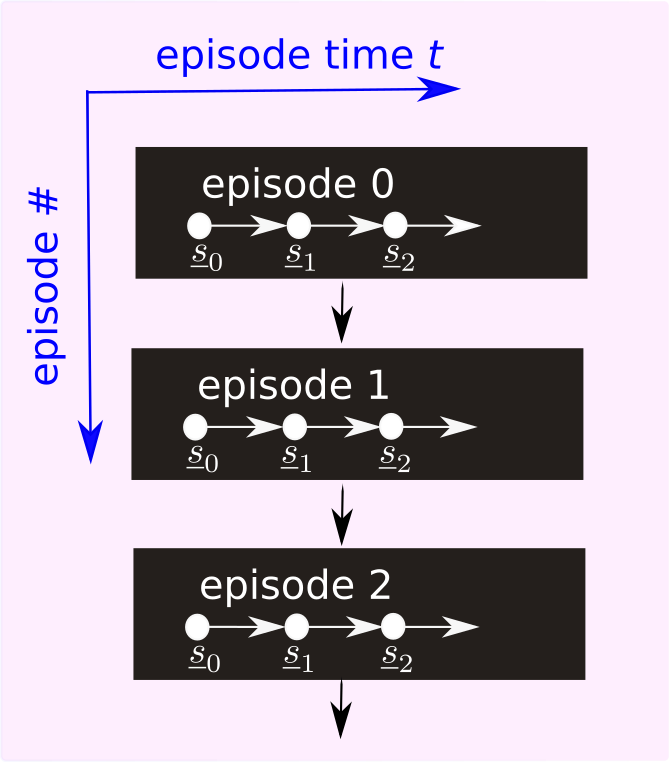
\includegraphics[width=3in]{RL/episodes.png}
\caption{Axes 
for episode time and episode number.} 
\label{fig-epi}
\end{figure}

I based this chapter on the following 
references. Refs.\cite{fox}\cite{levine}

In RL, we consider an ``agent" or
robot that
is learning. 

Let $T\in \ZZ_{>0}$ be the duration time
of an {\bf episode} of learning.
If $T=\infty$, we say that the episode
has an infinite time horizon.
A learning episode will 
 evolve
towards the right,
 for times $t=0,1, \ldots, T-1$. 
We will consider multiple learning episodes.
The episode number will
evolve from top to bottom.
This is illustrated in Fig.\ref{fig-epi}.

 Let $\rvs_t\in S_\rvs $ 
for $t\in [0,T-1]_\ZZ$ be random variables that record the {\bf state} of the
agent at various times $t$.

Let $\rva_t\in S_\rva$ for 
$t\in [0,T-1]_\ZZ$ be random variables that record the {\bf action} of the agent at various times $t$.

Let $\rvtheta_t\in S_\rvtheta$ 
for $t\in [0,T-1]_\ZZ$ be
random variables that record the
 {\bf policy parameters} 
at various times $t$.



For $\rvX\in \{\rvs, \rva, \rvtheta\}$, define $\rvX$ followed by a dot to be the vector 
\beq
\rvX. = 
[\rvX_0, \rvX_1, \ldots, \rvX_{T-1}]
\;.
\eeq
Also let
\beq
\rvX_{\geq t} = 
[\rvX_t, \rvX_{t+1}, \ldots, \rvX_{T-1}]
\;.
\eeq

\begin{figure}
\centering
$$\xymatrix{
\rvtheta_0\ar@/^1pc/[dd]&
\rvtheta_1\ar@/^1pc/[dd]&
\rvtheta_2\ar@/^1pc/[dd]&\\
\rvs_0\ar[r]\ar[d]\ar@/^1pc/[dd]&
\rvs_1\ar[r]\ar[d]\ar@/^1pc/[dd]&
\rvs_2\ar[d]\ar@/^1pc/[dd]\\
\rva_0\ar[ur]\ar[d]&
\rva_1\ar[ur]\ar[d]&
\rva_2\ar[d]
\\
\rvr_0&
\rvr_1&
\rvr_2
}$$
\caption{State-Action-Reward dynamical bnet}
\label{fig-basic-rl}
\end{figure}

Fig.\ref{fig-basic-rl} shows
the basic State-Action-Reward bnet
for an agent that is learning.
The TPMs for the
nodes of Fig.\ref{fig-basic-rl} are
given in blue below:

\beq\color{blue}P(a_t|s_t, \theta_t)\text{ = given.}
\eeq
 $P(a_t|s_t, \theta_t)$ is called  a
{\bf policy with parameter $\theta_t$.} 

\beq\color{blue}P(s_{t}|s_{t-1}, a_{t-1})
\text{ = given.}\eeq
$P(s_t|s_{t-1}, a_{t-1})$ is called the
 {\bf TPM of the model}.
$P(s_t|s_{t-1}, a_{t-1})$ reduces to $P(s_0)$ when $t=0$.

\beq\color{blue}
P(r_t|s_t, a_t)=\delta(r_t, r(s_t, a_t)))
\;.\eeq
$r:S_\rvs\times S_\rva\rarrow \RR$ 
is a given
 {\bf one-time reward function}.


Note that 
\beq
P(s., a.|\theta.)=\prod_{t=0}^{T-1}
\{
P(s_t|s_{t-1}, a_{t-1})
P(a_t|s_t, \theta_t)\}
\;.
\eeq
Define the {\bf all times reward} 
$\Sigma$ by

\beq
\Sigma(s., a.) = 
\sum_{t=0}^{T-1}\gamma^t r(s_t, a_t)
\;.
\eeq
Here $0<\gamma<1$. 
$\gamma$, called the {\bf discount rate},
is included to assure 
convergence of $\Sigma$ when
$T\rarrow \infty$. 
If $r(s_t, a_t)< K$ for all $t$, then
$\Sigma< K \frac{1}{1-\gamma}$.

Define the {\bf objective (i.e. goal)
 function}
$E\Sigma(\theta.)$ by

\beq
E\Sigma(\theta.)=
E_{\rvs., \rva.|\theta.}
\Sigma(\rvs., \rva.)=
\sum_{s., a.}
P(s., a.|\theta.)\Sigma(s., a.)
\eeq
The goal of RL  is to
maximize the 
objective function over
its parameters $\theta.$.
The parameters $\theta^*.$ that 
maximize the objective function 
are the optimum strategy:

\beq 
\theta.^* = \argmax_{\theta.}
E\Sigma(\theta.)
\eeq

\hrule
Define a {\bf future reward} for
 times $\geq t$ as:
\beq
\Sigma_{\geq t}((s_{t'},
 a_{t'})_{t'\geq t}) =
 \sum_{t'=t}^{T-1}\gamma^{t'-t} r(s_{t'}, a_{t'})
\eeq

Define the following {\bf expected conditional 
future rewards} (rewards for times 
$\geq t$,
conditioned on certain quantities
having given values):

\beqa
v_t &=& v(s_t, a_t; \theta.)=E_{\rvs., \rva.|s_t,a_t, \theta.}[\Sigma_{\geq t}]\\
V_t &=& V(s_t;\theta.)=E_{\rvs., \rva.|s_t, \theta.}[\Sigma_{\geq t}]=
E_{\rva_t|s_t, \theta.}[v(s_t, \rva_t;\theta.)]
\eeqa

$v$ is usually called $Q$
in the literature. We will
refer to $Q$ as $v$
in order to follow
a convention wherein an
$\rva_t$-average changes a lower case
letter to an upper case one.  

We will sometimes
write $v(s_t, a_t)$
instead of $v(s_t, a_t;\theta.)$.

Since $E\Sigma_{\geq t}$ only depends on
$\theta_{\geq t}$, $v(s_t, a_t;\theta.)=
v(s_t, a_t;\theta_{\geq t})$, and
$V(s_t;\theta.)=
V(s_t;\theta_{\geq t})$.

Note that the objective function 
$E\Sigma$ can be expressed in terms of 
$v_0$ by averaging over its unaveraged
parameters:
\beq
E\Sigma(\theta.)=
E_{\rvs_0,\rva_0|\theta_0}
v(\rvs_0, \rva_0;\theta.)
\eeq

Define
a {\bf one-time reward}
 and an 
{\bf expected conditional one-time  reward} as:
\beqa
r_t &=& r(s_t, a_t)\\
R_t &=& R(s_t;\theta_t)=
E_{\rva_t|s_t, \theta_t}[r(s_t, \rva_t)]\
\;.
\eeqa


\hrule

Note that

\beqa
\Sigma_{\geq t} &=& r_t + \gamma r_{t+1} 
+ \gamma^2 r_{t+2} +\ldots
+ \gamma^{T-1-t} r_{t+(T-1-t)}\\
&=& r_t + \gamma \Sigma_{\geq t+1}
\label{eq-Sigma}
;.
\eeqa

 
If we take
 $E_{\rvs., \rva.|s_t, a_t, \theta.}
[\cdot]$
of both sides of Eq.(\ref{eq-Sigma}), 
we get

\beq
v_t = r_t + \gamma E_{\rvs_{t+1},
 \rva_{t+1}|\theta.} [v_{t+1}]
\;.
\eeq
If we take $E_{\rvs., \rva.|s_t, \theta.}[\cdot]$
of both sides of Eq.(\ref{eq-Sigma}), 
we get

\beq
V_t = R_t + \gamma E_{\rvs_{t+1}|\theta.}
[V_{t+1}]
\;.
\eeq

Note that
\beqa
\Delta r_t&=& r_t -R_t\\
&=& r_t -(V_t - 
\gamma E_{\rvs_{t+1}|\theta.} [V_{t+1}])\\
&=& r_t
+ \gamma E_{\rvs_{t+1}|\theta.} [V_{t+1}]
-V_t
\;.
\eeqa
Define
\beq
\Delta v_t = v_t - V_t
\;. 
\eeq
Note that 
\beq
\Delta v_t = \Delta r_t
\;.
\eeq

Next, we will discuss 3 RL bnets
\begin{itemize}
\item
exact RL bnet 
(exact, assumes policy is known)
\item
Actor-Critic RL bnet (approximate, 
assumes
policy is known)
\item
Q function learning RL bnet (approximate, 
assumes
policy is NOT known)
\end{itemize}



\section{Exact RL bnet}

\begin{figure}
\centering
$$\xymatrix{
\rvtheta.\ar[d]\ar[dr]\ar[drr]\ar[drrr]
\ar@/_2pc/[dddddd]\\
\rvtheta_0\ar@/^1pc/[dd]&
\rvtheta_1\ar@/^1pc/[dd]&
\rvtheta_2\ar@/^1pc/[dd]&
\rvtheta_3&\\
\rvs_0\ar[r]\ar[d]\ar@/^1pc/[dd]&
\rvs_1\ar[r]\ar[d]\ar@/^1pc/[dd]&
\rvs_2\ar[r]\ar[d]\ar@/^1pc/[dd]&
\rvs_3\\
\rva_0\ar[d]\ar[ur]&
\rva_1\ar[d]\ar[ur]&
\rva_2\ar[d]\ar[ur]&
\rva_3\\
\rvr_0\ar[d]&
\rvr_1\ar[d]&
\rvr_2\ar[d]&
\rvr_3\\
\rvv_0(\cdot)\ar[d]&
\rvv_1(\cdot)\ar[l]&
\rvv_2(\cdot)\ar[l]&
\rvv_3(\cdot)\ar[l]\\
\rvtheta'.
}$$
\caption{Exact RL bnet. 
$v_t(\cdot)$ means the  array
$[v_t(s_t,a_t)]_{\forall s_t, a_t}$ 
The
following arrows 
are implicit:
 for all $t$, arrow
from $\rvtheta.\rarrow \rvv_t(\cdot)$.
We did not draw those arrows
so as not to clutter the diagram.}
\label{fig-exact-rl}
\end{figure}
An exact RL bnet is given by
 Fig.\ref{fig-exact-rl}.


Fig.\ref{fig-exact-rl} is the 
same as Fig.\ref{fig-basic-rl} but
 with more nodes added in order to
optimize the policy parameters.
Here are the TPMs, printed
in blue, 
for the nodes not already discussed
in connection to 
Fig.\ref{fig-basic-rl}.

 

\beq \color{blue}
P(\theta_t|\theta.) =
\delta(\theta_t, (\theta.)_t)
\eeq


\beq\color{blue}\forall (s_t, a_t):\;\;
P(v_t(s_t, a_t)|r_t, v_{t+1}(\cdot),\theta.)
=\delta(v_t(s_t,a_t), r_t + 
\gamma E_{\rvs_{t+1},\rva_{t+1}
|\theta.}[ v_{t+1}])
\eeq

\beq \color{blue}
P(\theta.'|\theta., v_0(\cdot))=
\delta(\theta'.,
\theta. + \alpha\partial_{\theta.}
\underbrace{E_{\rvs_0, \rva_0|\theta_0}
v(\rvs_0, \rva_0
;\theta.)}_{E\Sigma(\theta.)})
\eeq
$\alpha>0$ is called the
{\bf learning rate}. This method
of improving $\theta.$ is 
called gradient ascent.

Concerning the
gradient of the
objective function, note that

\beqa
\partial_{\theta_t}E\Sigma(\theta.)&=&
\sum_{s., a.}
\partial_{\theta_t}P(s., a.|\theta.)
\Sigma(s., a.)\\
&=& 
\sum_{s., a.}P(s., a.|\theta.)
\partial_{\theta_t}
\ln P(s., a.|\theta.)\Sigma(s., a.)
\\
&=&
E_{\rvs., \rva.|\theta.}\left\{
\partial_{\theta_t}
\ln P(a_t|s_t, \theta_t)
\Sigma(s., a.)
\right\}
\;.
\eeqa
If we run the
agent $nsam(\vecs_t)$
times and obtain
samples $s_t[i], a_t[i]$ for all $t$ and
for $i=0, 1, \ldots,nsam(\vecs_t)-1$, 
we can express this  gradient as
follows:

\beq
\partial_{\theta_t}E\Sigma(\theta.)
\approx
\frac{1}{nsam(\vecs_t)}
\sum_{i}\sum_{t=0}^{T-1}
\partial_{\theta_t}
\ln P(a_t[i]\cond s_t[i], \theta_t)
r(s_t[i], a_t[i])
\;.
\label{eq-grad-samples}
\eeq

The exact RL bnet 
Fig.\ref{fig-exact-rl} is difficult to
use to calculate the
optimum parameters $\theta^*.$.
The problem 
is that $\rvs_t$
propagates towards the future
and the $\rvv_t(\cdot)$
propagates towards the past,
so we don't have a Markov Chain 
with a chain link for each $t$ (i.e., 
a
dynamical bnet) in the 
episode time direction.
Hence,
people have come up
with approximate RL bnets
that are
doubly dynamical (i.e.,
dynamical along
the episode time and
episode number axes.)
We discuss some of those
approximate RL bnets next. 



\section{Actor-Critic RL bnet}

For the actor-critic RL 
bnet, 
we approximate Eq.(\ref{eq-grad-samples})
by

\beq
\partial_{\theta_t}E\Sigma(\theta.)
\approx
\frac{1}{nsam(\vecs)}
\sum_{i}\sum_{t=0}^{T-1}
\underbrace{
\partial_{\theta_t}
\ln P(a_t[i]\cond s_t[i], \theta_t)
}_{Actor}
\underbrace{
\Delta r_t(s_t[i], a_t[i])
}_{Critic}
\eeq


\begin{figure}
\centering
$$\xymatrix{
\rvtheta_0\ar@/^1pc/[dd]\ar@/_1pc/[ddddd]&
\rvtheta_1\ar@/^1pc/[dd]\ar@/_1pc/[ddddd]&
\rvtheta_2\ar@/^1pc/[dd]\ar@/_1pc/[ddddd]&
\rvtheta_3\\
\vec{\rvs}_0\ar[r]\ar[d]\ar@/^1pc/[dd]
\ar@/^2pc/[ddd]&
\vec{\rvs}_1\ar[r]\ar[d]\ar@/^1pc/[dd]
\ar@/^2pc/[ddd]\ar[dddl]&
\vec{\rvs}_2\ar[r]\ar[d]\ar@/^1pc/[dd]
\ar@/^2pc/[ddd]\ar[dddl]&
\vec{\rvs}_3\ar[dddl]\\
\vec{\rva}_0\ar[d]\ar[ur]\ar@/^1pc/[dd]&
\vec{\rva}_1\ar[d]\ar[ur]\ar@/^1pc/[dd]&
\vec{\rva}_2\ar[d]\ar[ur]\ar@/^1pc/[dd]&
\vec{\rva}_3\\
\vec{\rvr}_0&
\vec{\rvr}_1&
\vec{\rvr}_2&
\vec{\rvr}_3\\
\ul{\Delta \vec{v}}_0\ar[d]&
\ul{\Delta \vec{v}}_1\ar[d]&
\ul{\Delta \vec{v}}_2\ar[d]&
\ul{\Delta \vec{v}}_3\\
\rvtheta'_0&
\rvtheta'_1&
\rvtheta'_2&
\rvtheta'_3
}$$
\caption{Actor-Critic RL bnet.  }
\label{fig-ac-rl}
\end{figure}
The actor-critic RL bnet
is given by Fig.\ref{fig-ac-rl}. This
bnet is approximate and assumes
that the policy is known. The
TPMs for its nodes
are given in blue below.



\beq\color{blue}
P(\theta_t) \text{ = given}
\eeq

\beq\color{blue}
P(s_t[i]\cond s_{t-1}[i], a_{t-1}[i]) = \text{ given} 
\eeq

\beq\color{blue}
P(a_t[i]\cond s_t[i], \theta_t)= \text{ given}
\eeq

\beq\color{blue}
P(r_t[i]\cond s_t[i],a_t[i])=
\delta(r_t[i],r(s_t[i], a_t[i]))
\eeq
$r:S_\rvs\times S_\rva\rarrow\RR $ is given.

\beq\color{blue}
P(\Delta v_t[i]\cond s_t[i], a_t[i], s_{t+1}[i])=
\delta(\Delta v_t[i], r(s_t[i], a_t[i]) +
\gamma \hat{V}(s_{t+1}[i];\phi')
- \hat{V}(s_t[i]);\phi)
\;.
\eeq

\beq\color{blue}
P(\theta'.)=\delta(\theta'.,
\theta_t +
\alpha \partial_{\theta_t}\sum_i
\ln P(a_t[i]\cond s_t[i], \theta_t )
\Delta v_t[i])
\eeq

$\hat{V}(s_t[i]);\phi)$ is
obtained by curve fitting
 (see Chapter \ref{ch-basic-fit})
using samples $(s_t[i], a_t[i])$ 
$\forall t,i$
with

\beq
 y[i]=\sum_{t'=t}^{T}
r(s_{t'}[i],a_{t'}[i])
\label{eq-V-approx}
\eeq
and 

\beq
\hat{y}[i]=
\hat{V}(s_t[i];\phi)
\;.
\eeq
Eq.(\ref{eq-V-approx}) 
is an approximation
because $(s_{t'}, a_{t'})_{t'>t}$ 
are averaged over in the exact
expression for $V(s_t)$.
$\hat{V}(s_{t+1}[i]);\phi')$ is
obtained in the same way as
$\hat{V}(s_t[i]);\phi)$
but with $t$ replaced by $t+1$
and $\phi$ by $\phi'$.

\section{Q function learning RL bnet}

\begin{figure}
\centering
$$\xymatrix{
\rvs_0\ar[r]\ar[d]
\ar@/^1pc/[dd]&
\rvs_1\ar[r]\ar[d]
\ar@/^1pc/[dd]&
\rvs_2\ar[r]\ar[d]
\ar@/^1pc/[dd]&
\rvs_3\\
\rva_0\ar[d]\ar[ur]&
\rva_1\ar[d]\ar[ur]&
\rva_2\ar[d]\ar[ur]&
\rva_3\\
\rvr_0&
\rvr_1&
\rvr_2&
\rvr_3\\
\rvQ_0(\cdot)\ar@/_1pc/[uu]\ar[r]&
\rvQ_1(\cdot)\ar@/_1pc/[uu]\ar[r]&
\rvQ_2(\cdot)\ar@/_1pc/[uu]\ar[r]&
\rvQ_3(\cdot)
}$$
\caption{Q function learning  RL bnet. }
\label{fig-learn-q}
\end{figure}
The Q-function learning RL bnet
is given by Fig.\ref{fig-learn-q}. This
bnet is approximate and assumes
that the policy is NOT known. The
TPMs for its nodes
are given in blue below. (Remember
that $Q=v$).

\beq\color{blue}
P(s_t|s_{t-1}, a_{t-1}) = \text{ given} 
\eeq



\beq\color{blue}
P(a_t|s_t, v_t(\cdot))=
\delta(a_t, \argmax_{a}v_t(s_t, a))
\eeq

\beq\color{blue}
P(r_t|s_t,a_t)=\delta(r_t, r(s_t, a_t))
\eeq
$r:S_\rvs\times S_\rva\rarrow\RR $ is given.

\beqa\color{blue}\forall (s_t, a_t):\;\;
\lefteqn{P(v_t(s_t, a_t)| 
v_{t-1}(\cdot))=}\nonumber
\\
&\color{blue}=&\color{blue}
\delta(v_t(s_t, a_t), 
r(s_{t}, a_{t})+ \gamma \text{max}_{a}
E_{\rvs_{t+1}|s_{t}, a_{t}}
v_{t-1}(\rvs_{t+1}, a))
\label{eq-sprime-av}
\eeqa
This 
value for $v_t(s_t, a_t)$
approximates $v_t = r_t +\gamma 
E_{\rvs_{t+1}, \rva_{t+1}}v_{t+1}$.

Some people 
use the bnet of 
Fig.\ref{fig-learn-q-approx})
instead of Fig.\ref{fig-learn-q}
and replace 
 Eq.(\ref{eq-sprime-av})
by

\beqa\color{blue}\forall (s_t, a_t):\;\;
\lefteqn{P(v_t(s_t, a_t)| s_{t+1},
v_{t-1}(\cdot))=}\nonumber
\\
&\color{blue}=&\color{blue}
\delta(v_t(s_t, a_t), 
r(s_{t}, a_{t})+ \gamma \text{max}_{a}
v_{t-1}(s_{t+1}, a))
\;.
\eeqa



\begin{figure}
\centering
$$\xymatrix{
\rvs_0\ar[r]\ar[d]
\ar@/^1pc/[dd]&
\rvs_1\ar[r]\ar[d]
\ar@/^1pc/[dd]
\ar[lddd]&
\rvs_2\ar[r]\ar[d]
\ar@/^1pc/[dd]
\ar[lddd]&
\rvs_3
\ar[lddd]\\
\rva_0\ar[d]\ar[ur]&
\rva_1\ar[d]\ar[ur]&
\rva_2\ar[d]\ar[ur]&
\rva_3\\
\rvr_0&
\rvr_1&
\rvr_2&
\rvr_3\\
\rvQ_0(\cdot)\ar@/_1pc/[uu]\ar[r]&
\rvQ_1(\cdot)\ar@/_1pc/[uu]\ar[r]&
\rvQ_2(\cdot)\ar@/_1pc/[uu]\ar[r]&
\rvQ_3(\cdot)
}$$
\caption{Q function learning  RL bnet.
Same as Fig.\ref{fig-learn-q}
but with new arrow
passing $s_t$ to $Q_{t-1}$. }
\label{fig-learn-q-approx}
\end{figure}
\chapter{Reliability Box Diagrams and Fault 
Tree Diagrams}
This chapter is based on
Refs.\cite{reliasoft}
and \cite{ftree-manual}.

In this chapter, we assume that
reader is familiar
with
Boolean Algebra. See 
 Chapter \nameref{ch-conventions}
for a quick review 
of what
we recommend that you know about
Boolean Algebra
to fully appreciate this chapter.

\begin{figure}[h!]
\centering
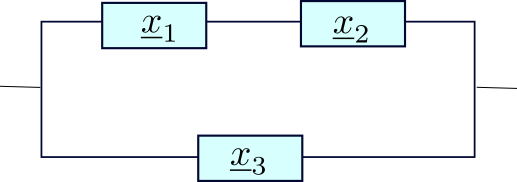
\includegraphics[width=3in]
{reliability/relia-example.png}
\caption{Example of rbox diagram.} 
\label{fig-relia-rbox}
\end{figure}

\begin{figure}[h!]
\centering
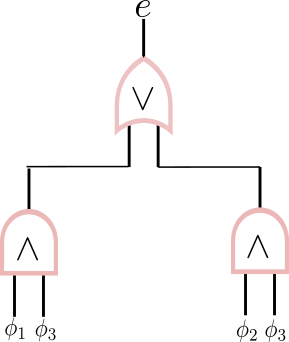
\includegraphics[width=1.5in]
{reliability/relia-ftree.png}
\caption{An ftree diagram equivalent to
Fig.\ref{fig-relia-rbox}. It
represents 
$e=(\phi_1\A \phi_3)\V(\phi_2\A\phi_3)$. } 
\label{fig-relia-ftree}
\end{figure}

\begin{figure}[h!]
\centering
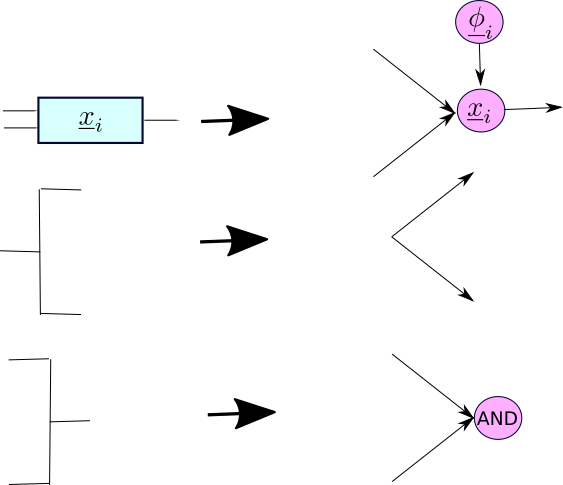
\includegraphics[width=3in]
{reliability/relia-map.png}
\caption{How to map an rbox diagram to a bnet.} 
\label{fig-relia-map}
\end{figure}

\begin{figure}[h!]
\centering
$$\xymatrix@-.5pc{
&\ul{\phi}_1\ar[d]&&\ul{\phi}_2\ar[d]
\\
&\rvx_1\ar[rr]
&&
\rvx_2
\ar `r[rd][rd]
\\
\rvb\ar`u[u][ru]
\ar`d[dr][rrd]
&&&&\rvA\ar[r]&\rve
\\
&&
\rvx_3
\ar `r[rru][rru]
\\
&&\ul{\phi}_3\ar[u]
}$$
\caption{bnet corresponding
the rbox diagram 
Fig.\ref{fig-relia-rbox}.}
\label{fig-relia-bnet}
\end{figure}

Complicated devices
with a large number 
of components
such as airplanes or rockets can
fail in many
ways. If
their performance
depends 
on some components
working in series
and one 
of the components
in the series
fails, this
may lead to
catastrophic failure.
To avert
such disasters,
engineers use equivalent
components
connected in parallel
instead of in series,
thus providing multiple backup
systems. They
analyze the
device to find its 
weak points and add
backup capabilities 
there. They also
estimate the
average time to failure
for the device. 



The two 
most popular diagrams
for finding the failure modes and their rates
for large complicated devices
are
\begin{itemize}
\item
rbox diagrams = Reliability Box diagrams. 
See Fig.\ref{fig-relia-rbox} for an example.
\item
ftree diagrams = Fault Tree Diagrams.
See Fig.\ref{fig-relia-ftree} for an example.
\end{itemize}
In an ftree diagram,
several nodes might
stand for the same 
component of a physical device.
In an rbox diagram,
on the
other hand, 
each node
represents a distinct  component
in a device. Hence, rbox diagrams
resemble the device they are
addressing
whereas ftree diagrams don't.
Henceforth, we will
refer to this desirable property
as {\bf  physical resemblance}.

As we will
show below with an example,
it is pretty
straightforward
to translate
an rbox to  an ftree diagram.
Going the other
way, translating
an ftree to an rbox diagram
is much more difficult.



Next we will define
a new kind of bnet
that we will call a failure bnet
that has physical resemblance.
Then we will describe
a simple method of translating (i.e., mapping)
any rbox diagram to a failure bnet.
Then we will show
how a failure
bnet can be used
to do all the
calculations
that are normally
done with an rbox
or an ftree diagram.
In that sense,
failure bnets
seem to afford
all the benefits
of both ftree and rbox 
diagrams.


A {\bf failure bnet} contains
nodes of 5  types,
labeled $\rvb$, $\rve$, $\rvx_i$,
$\ul{\phi}_i$, and $\rvA_i$.
All nodes have only
two possible states
$S=Success=0$, $F=Failure=1$.
\begin{enumerate}
\item 
The bnet has a beginning node labeled
$\rvb$ which is always set to success.
The $\rvb$ node
and the $\ul{\phi}_i$
nodes are the only root nodes of
the bnet.

\item The bnet has 
a single leaf node, the end node, labeled 
$\rve$. $\rve$ is fixed.
In rbox diagrams,
$\rve=S$
whereas in ftree diagrams, $\rve=F$.

\item
$\rvx^{nx}=
(\rvx_0, \rvx_1, \ldots, \rvx_{nx-1})$.
$\rvx_i\in \{S, F\}$ for all $i$.

Suppose $\rvx_i$
has parents 
$\ul{\phi}_i$ and $\rva^{na}=(\rva_0, \rva_1,
\dots \rva_{na-1})$.
Then the TPM of node $\rvx_i$ is
defined to be

 
\beq\color{blue}
P(x_i|\phi_i,a^{na})=
\delta(x_i,\phi_i\V  \V_{i=0}^{na-1} a_i)
\eeq

\item
For each node $\rvx_i$, the bnet has
 a ``performance"
 root node $\ul{\phi}_i\in \bool$
with an arrow
pointing from it 
to $\rvx_i$ (i.e, 
$\ul{\phi}_i\rarrow \rvx_i$).
For all $i$,

\beq \color{blue}
P(\phi_i)=
\eps_i \delta(\phi_i, F)
+\ol{\eps}_i\delta(\phi_i, S)
\;.
\eeq
$\eps_i$ is the failure probability
and $\ol{\eps}_i=1-\eps_i$
is the success probability.
We name the failure
probability $\eps_i$
because it
is normally very small.
It is usually
set to
$1-e^{-\lam_it}\approx \lam_it$
when $\lam_it<<1$,
where $\lam_i$
is the failure rate
for node $\rvx_i$
and $t$ stands for time.
The rblock
literature
usually calls 
$\ol{\eps_i}=R_i$
the {\bf reliability}
 of 
node $\rvx_i$,
and 
$\eps_i=(1-R_i)=F_i$
its {\bf unreliability}.


\item
The nodes $\rvA_i\in \bool$ 
are simply AND gates.
If $\rvA_i$ has inputs $\rvy^{ny}=
(\rvy_0, \rvy_1,
\ldots, \rvy_{ny-1})$,
then the TPM of $\rvA_i$ is

\beq\color{blue}
P(A_i|y^{ny})=
\delta(A_i, \A_{i=0}^{ny-1}y_i)
\;.
\eeq

\end{enumerate}

An instance (instantiation)
of a bnet is the bnet 
with all nodes set to
a specific state.
A {\bf realizable instance (r-instance)}
of a bnet is one
which has non-zero probability.

Fig.\ref{fig-relia-map}
shows how to translate
any rbox diagram
to a failure bnet.
To illustrate this procedure,
we translated the rbox diagram
Fig.\ref{fig-relia-rbox}
into the failure bnet 
Fig.\ref{fig-relia-bnet}.

For the
failure bnet 
Fig.\ref{fig-relia-bnet},
one has:

\beq
\begin{array}{l}\color{blue}
P(b)=\indi(b=0)\\\color{blue}
P(x_1|\phi_1, b)=\indi(x_1=\phi_1\V b)\\\color{blue}
P(x_2|\phi_2, x_1)=\indi(x_2=\phi_2\V x_1)\\\color{blue}
P(x_3|\phi_3, b)=\indi(x_3=\phi_3\V b)\\\color{blue}
P(A|x_2, x_3)e=\indi(x_2\A x_3)\\\color{blue}
P(e|A)=\indi(e=A)
\end{array}
\;.
\eeq
Therefore, all r-instances
of this bnet  must
satisfy

\beqa
e&=&(\phi_1\V\phi_2)\A \phi_3
\\
&=&(\phi_1\A \phi_3)\V(\phi_2\A\phi_3)
\;.
\label{eq-ftree}
\eeqa
Eq.(\ref{eq-ftree})
proves that 
Fig.\ref{fig-relia-ftree}
is indeed a 
representation 
of Fig.\ref{fig-relia-rbox}.

Next, we consider 
r-instances of this bnet for 
two cases: $e=S$ and $e=F$.

\begin{itemize}
\item {\bf rblock analysis: $e=S=0$.}\\
Table \ref{tab-probs-end-0}
shows the
probability of all possible r-instances
that end in success
for the failure bnet Fig.\ref{fig-relia-bnet}.
(These r-instances are
the main focus of rblock analysis).
The first 4 of
those probabilities (those with
$\phi_3=0$) sum to $\ol{\eps}_3$
so the sum $P(e=S)$ of all 
5 is

\beq
P(e=S)=\ol{\eps}_3
+ \ol{\eps}_1\ol{ \eps}_2 \eps_3
\;,
\eeq
or, expressing
it in reliability language
in which $\ol{\eps}=R$,

\beq
P(e=S)=R_3
+ R_1 R_2 \ol{R}_3
\;.
\eeq


% using array package and
%\begin{tabular}{|m{5cm}|m{2cm}|} for next table



% Please add the following required packages to your document preamble:
% \usepackage[table,xcdraw]{xcolor}
% If you use beamer only pass "xcolor=table" option, i.e. \documentclass[xcolor=table]{beamer}
\begin{table}[]
\centering
\begin{tabular}{|m{5cm}|m{2cm}|}
\hline
\rowcolor[HTML]{ECF4FF} 
instance & probability \\ \hline
$\rbd{0}{1}{0}{0}$ & $\ol{\eps}_1 \eps_2\ol{\eps}_3$ \\ \hline
$\rbd{1}{0}{0}{0}$ & $\eps_1 \ol{\eps}_2 \ol{\eps}_3$ \\ \hline
$\rbd{1}{1}{0}{0}$ & $\eps_1\eps_2\ol{\eps}_3$ \\ \hline
$\rbd{0}{0}{0}{0}$ & $\ol{\eps}_1 \ol{\eps}_2 \ol{\eps}_3$ \\ \hline
$\rbd{0}{0}{1}{0}$ & $\ol{\eps}_1\ol{\eps}_2\eps_3$ \\ \hline
\end{tabular}
\caption{Probabilities of all possible
 r-instances with $e=S=0$ for failure bnet
 Fig.\ref{fig-relia-bnet}.}
\label{tab-probs-end-0}
\end{table}


\item {\bf ftree analysis: $e=F=1$.}\\
Table \ref{tab-probs-end-1}
shows the
probability of all possible r-instances
that end in failure
for the failure bnet Fig.\ref{fig-relia-bnet}.
(These r-instances are
the main focus of ftree analysis).
If we set 
 $\eps_i=\eps$
and $\ol{\eps}_i\approx 1$
for $i=1,2,3$, then the first
two of those r-instances
have probabilities of $order(\eps^2)$
and the third has probability of
$order(\eps^3)$.
The two lowest order ($order(\eps^2)$)
r-instances
are called the ``minimal cut sets"
of the ftree. 
We will have more to say 
about minimal cut sets later on.
For now,
just note
from Eq.(\ref{eq-ftree})
that the ftree Fig.\ref{fig-relia-ftree}
is just the result
of joining
together with ORs
two expressions, one for each 
of the
two minimal cut sets.




% Please add the following required packages to your document preamble:
% \usepackage[table,xcdraw]{xcolor}
% If you use beamer only pass "xcolor=table" option, i.e. \documentclass[xcolor=table]{beamer}
\begin{table}[]
\centering
\begin{tabular}{|m{5cm}|m{2cm}|}
\hline
\rowcolor[HTML]{ECF4FF} 
instance & probability \\ \hline
$\rbd{0}{1}{1}{1}$ & $\ol{\eps}_1 \eps_2\eps_3$ \\ \hline
$\rbd{1}{0}{1}{1}$ & $\eps_1 \ol{\eps}_2 \eps_3$ \\ \hline
$\rbd{1}{1}{1}{1}$ & $\eps_1\eps_2\eps_3$ \\ \hline
\end{tabular}
\caption{Probabilities of all possible 
r-instances with $e=F=1$ for  the failure bnet
 Fig.\ref{fig-relia-bnet}.}
\label{tab-probs-end-1}
\end{table}

\end{itemize}

\hrule\noindent
{\bf More general $\rvx_i$.}\\
Failure bnets can actually
accommodate
$\rvx_i$ nodes
of a more general
kind than what we first stipulated.
Here are some possibilities: 



For any $a^n\in\bool^n$, let
\beq
len(a^n)=\sum_i a_i
\eeq

\begin{itemize}
\item {\bf OR gate}

\beqa\color{blue}
P(x_i|\phi_i,a^{na})&=&\color{blue}
\delta(x_i, \phi_i\V\V_j a_j)
\\
&=& \color{blue}
\delta(x_i, \phi_i\V\indi(len(a^{na})>0))
\eeqa

\item {\bf AND gate}

\beqa\color{blue}
P(x_i|\phi_i,a^{na})&=&\color{blue}
\delta(x_i, \phi_i\V\A_j a_j)
\\
&=& \color{blue}
\delta(x_i, \phi_i\V\indi(len(a^{na})=na))
\eeqa

\item {\bf Fail if least  $K$ failures
(less than $K$ successes)}

\beq\color{blue}
P(x_i|\phi_i,a^{na})=
\delta(x_i, \phi_i\V\indi(len(a^{na})\geq K))
\eeq

\item {\bf Fail if less than $K$ failures (at
least $K$ successes)}

\beq\color{blue}
P(x_i|\phi_i,a^{na})=
\delta(x_i, \phi_i\V\indi(len(a^{na})< K))
\eeq

\item {\bf Fail if exactly one failure}

\beq\color{blue}
P(x_i|\phi_i,a^{na})=
\delta(x_i, \phi_i\V\indi(len(a^{na})=1))
\eeq
This equals an XOR (exclusive OR)
gate when $na=2$.

\item {\bf General gate}\\
$f:\bool^{na}\rarrow \bool$

\beq\color{blue}
P(x_i|\phi_i,a^{na})=
\delta(x_i, \phi_i\V f(a^{na}))
\eeq
 
\end{itemize}
\hrule
\section{Minimal Cut Sets}

Suppose $x\in\bool$ and $f:\bool\rarrow \bool$.
Then
by direct evaluation, we see that

\beq
f(x)=[\ol{x}f(0)]\V [xf(1)]
\;.\label{eq-or-f}
\eeq
Let

\beq
\begin{array}{l}
!x=1-x,\\
!^0x=x,\\
!^1x=!x
\end{array}
\eeq
Then Eq.(\ref{eq-or-f})
can be rewritten as
 
\beq
f(x)= \V_{a\in\bool} [(!^{\ol{a}}x) f(a)]
\label{eq-ors-of-ands-1}
\;.
\eeq
Now suppose $x^n\in \bool^n$
and $f:\bool^n\rarrow \bool$.
Eq.(\ref{eq-ors-of-ands-1})
generalizes to

\beq
f(x^n)= \V_{a^n\in\bool^n}
 [\prod_i(!^{\ol{a}_i}x_i) f(a^n)]
\label{eq-ors-of-ands-n}
\;.
\eeq
Eq.(\ref{eq-ors-of-ands-n})
is called an {\bf ors-of-ands} normal form 
expansion.
There is also an {\bf ands-of-ors} normal
form expansion 
obtained by swapping multiplication
and $\V$
in Eq.(\ref{eq-ors-of-ands-n}), 
but we won't need it here.

A {\bf cut
set} is a set
of $\phi_i$'s such that
if they are all equal to $F$,
then $e=F$ for all the
r-instances.
A {\bf minimal cut set}
is a cut set such that there
are no larger cut sets that contain it.
From the failure bnet,
we can always find 
a function $f:\bool^{nx}\rarrow\bool$
such that
$e=f(\phi^{nx})$
for all the r-instances.
We did that for our
example failure
bnet and obtained Eq.(\ref{eq-ftree}).
We can
then
express 
$f(\phi^{nx})$ as an ors-of-ands expansion
to find all the minimal cut sets.
The ands
terms in that ors-of-ands
expansion 
each gives
a different minimal cut set,
after some simplification.
The ors-of-ands
expression
is not unique
and it may be necessary to simplify 
(using the Boolean Algebra identities
given in Chapter \nameref{ch-conventions})
to remove those redundancies.
\chapter{Restricted Boltzmann Machines}
In what follows, we will
abbreviate \qt{restricted Boltzmann machine}
by rebo.

Let

$v\in \{0,1\}^{nv}$

$h\in \{0,1\}^{nh}$

$b\in \RR^{nv}$ (mnemonic, $v$ and $b$
sound the same)

$a\in \RR^{nh}$

$W^{v|h}\in \RR^{nv\times nh}$

Energy:
\beq
E(v,h)= -(b^Tv + a^Th + v^T W^{v|h} h)
\eeq

Boltzmann distribution:
\beq
P(v,h)=
\frac{e^{-E(v,h)}}
{Z}
\eeq

Partition function:
\beq
Z=\sum_{v,h}e^{-E(v,h)}=Z(a,b,W^{v|h})
\eeq

\beqa
P(v|h)&=&
\frac{e^{b^Tv+a^Th + v^T W^{v|h}h}}
{\sum_ve^{b^Tv+a^Th + v^T W^{v|h}h}}
\\&=&
\frac{e^{b^Tv + v^T W^{v|h}h}}
{\sum_v e^{b^Tv+ v^T W^{v|h}h}}
\\
&=&
\prod_i\frac{ e^{v_i(b_i
+ \sum_jW^{v|h}_{i,j}h_j)}}
{\sum_{v_i=0,1}e^{v_i(b_i
+ \sum_j W^{v|h}_{i,j}h_j)}}\\
&=&
\prod_i P(v_i|h)
\eeqa


\beq
P(v_i|h)=
\frac{e^{v_i(b_i
+ \sum_jW^{v|h}_{i,j}h_j)}}{Z_i(h)}
\label{eq-pv}
\eeq

Eq.(\ref{eq-pv})
implies that a rebo
can be
represented by the bnet
Fig.\ref{fig-rebo}.

\begin{figure}[h!]
\centering
$$\xymatrix{
\rvh\ar[d]\ar[dr]\ar[drr]\\
\rvv_0 & \rvv_1 &\rvv_2
}$$
\caption{
bnet for a Restricted 
Boltzmann Machine (rebo)
with $nv=3$}
\label{fig-rebo}
\end{figure}

Let
\beq
x_i=b_i+\sum_j W^{v|h}_{ij}h_j
\;.
\eeq
Then

\beqa
P(v_i=1|h)&=&
\frac{e^{x_i}}
{1 + e^{x_i}}\\
&=&
\frac{1}
{1 + e^{-x_i}}\\
&=&
\smoid(x_i)
\;.
\eeqa

One could
also expand the node $\rvh$
in Fig.\ref{fig-rebo}
into $nh$ nodes.
But note that $P(h)\neq \prod_jP(h_j)$
so there would be arrows among the $h_j$ 
nodes.

Note that the rebo bnet
is a special case of Naive Bayes
(See Chapter \ref{ch-naive}) with
$v_i, h_i\in\{0,1\}$
and specific $P(h)$
and $P(v_i|h)$ node matrices.
\chapter{Scoring the Nodes of a Learned Bnet}
\label{ch-scoring}

Chapter \ref{ch-struc-learn}
discusses how 
to learn a bnet  from data.
Many algorithms for
doing this require scoring
how well
a particular bnet fits
the data.
This chapter 
is an introduction to
such scoring.

Normally,
each node of a bnet
is scored separately,
and then those node scores are summed
to get the bnet score.

In this chapter,
scores are defined 
so that a higher score
means a better fit.
By taking
the negative
of such a score,
one can 
always get a score
such that a lower score means a
 better fit.

There are 2 main types of
bnet scores: Maximum Likelihood (ML) scores,
and Shannon Information Theory (SIT)
scores.
For an ML score,
one takes
the log
of a maximum
likelihood function $P(x|\theta)$:

\beq
\text{ML-score}=\ln(P(x|\theta))
\;,
\eeq
and for a SIT score, 
one averages over the ML score
to get a negative entropy:

\beq
\text{Info-score}
=\sum_x P(x|\theta)\ln P(x|\theta)
=
-H(P_{\rvx|\theta})
\;.
\eeq
Thus, one maximizes a 
likelihood function
or minimizes its entropy,
to obtain the same thing, namely,
a good estimate of the
hidden parameters $\theta$. 

\section*{
Probability Distributions
and Special Functions}

While
writing
this chapter,
I briefly consulted 
the following Wikipedia articles
about
the definitions
and properties of
certain
probability
distributions
and special
functions.
\begin{itemize}
\item
Categorical Distribution,
 Ref.\cite{wiki-categorical}
\item
Multinomial Distribution,
 Ref.\cite{wiki-multi-dist}
\item
Dirichlet Distribution, 
Ref.\cite{wiki-diri}
\item 
Multivariate Normal Distribution,
Ref.\cite{wiki-multi-normal}

\item
Beta function, 
Ref.\cite{wiki-beta-fun}
\item
Multinomial Coefficients,
 Ref.\cite{wiki-multi-thm}
\item 
Gamma Function
Ref.\cite{wiki-gamma-fun}
\end{itemize}

Here are a few 
results 
from those Wikipedia
articles that we
will use later on
in this chapter.

Below,
we will abbreviate
$q_+=\sum_i q_i$, and
$q.=(q_0, q_1, \ldots, q_{nq-1})$
for various quantities $q$

{\bf Gamma function}. If $n>0$ is an integer,
\beq
\Gamma(n+1)=n!
\eeq

The {\bf multivariate Beta function} 
is defined by
\beq
B(\alp.)=
\frac{\prod_k\Gamma(\alp_k)}
{\Gamma(\alp_+)}
\eeq
where $\alp_k>0$ for all $k$.

The {\bf multinomial coefficient}
is defined by
\beq
C(N.)=
\frac{N_+!}{\prod_k N_k!}
\eeq
where $N_k$ are non-negative
integers.

The {\bf inverse of the multinomial 
coefficient} will
be denoted by
\beq
CI(N.)
=
\frac{1}{C(N.)}
=
\frac{\prod_k N_k!}{N_+!}
\eeq

The {\bf Categorical Distribution}
is defined by
\beq
Cat(x; \pi.)
=\pi_x=
\prod_{k} \pi_k^{\indi(k=x)}
\eeq
for $k, x\in S_\rvx$,
where 
$\pi.$ is a
probability dist.(i.e., $\pi_k\geq 0$
for all $k$,
and $\pi_+=1$).



The {\bf Multinomial Distribution}
is defined by
\beq
Mul(N.;\pi., N)
=
C(N.)
%\prod_k \pi_k^{N_k}
\;,
\eeq
where $N_k$
is a non-negative
integer for all $k$,
$N_+=N$,
and $\pi.$
is a probability dist.
Mul() satisfies:
\beq
E[\ul{N_k}]=N\pi_k
\;.
\label{eq-exp-val-mul}
\eeq

The {\bf Dirichlet Distribution}
is defined by
\beq
Dir(\pi.;\alp.)=
\frac{1}{B(\alp.)}
\prod_k
\pi_k^{\alp_k-1}
\eeq
where $\alp_k>0$
for all $k$,
and $\pi.$
is a probability dist.
The
$\alp.$ are called 
{\bf concentration parameters}
or {\bf hyperparameters}.
Dir() satisfies:
\beq
E[\ul{\pi_k}]=\frac{N_k}{N_+}
\;.
\label{eq-exp-val-dir}
\eeq


\hrule\noindent
Dir() is {\bf conjugate prior} of  Mul()

Note that

\beq
Mul(N.;\pi., N)Dir(\pi.;\alp.)
=
\calk( N.,\alp.)
Dir(\pi.;N.+\alp.)
\;,
\eeq
where

\beq
\calk(N., \alp.)=
\frac{B(N.+\alp.)}
{CI(N.)B(\alp.)}
\;.
\eeq
\hrule\noindent
Dir() is replaceable by a Mul()
for large concentration parameters

Note that if $N_k$ is a positive  integer
and
$\alp_k=N_k+1$ for all $k$, then

\beqa 
Dir(\pi.;\alp_k=N_k+1)
&=&
C(N.)\prod_k \pi_k^{N_k}
\\
&=&
Mul(N.; \pi., N_+)
\;.
\eeqa

\section*{Single node with no parents}
In this
section,
we consider a 
learned bnet
consisting of
a single node with
no parents.
We will consider
arbitrary
learned
bnets
in the next section.
But we start with 
this simplified
case so as to reduce
the number of indices
in most quantities
from 3 to 1.
All the results
that we derive
in this section
will
be used in the next 
section
after 
adding the extra indices.
This way,
we will
avoid
carrying
the extra indices
throughout
the intermediate steps
of many derivations.

For state
$k\in\{0, 1, \ldots, 
nk-1\}$
of a single node $\rvx$, let


$\rvN_k$=
current count number
(an integer, data)

$\ul{\pi}.$=
a probability dist, the TPM for the node

$\ul{\alp}_k$=
prior count
number



\begin{figure}[h!]
$$
\xymatrix{
\rvN.&\ul{\pi.}\ar[l]&
\ul{\alp.}\ar[l]
}$$
\caption{
For a bnet
consisting
of a single node
with no parents, 
this is a
Markov chain of
current counts ($\rvN.$), TPM ($\ul{\pi.}$),
and
prior counts ($\ul{\alp.}$)
.}
\label{fig-n-pi-alp-single}
\end{figure}

Consider
the Markov chain
bnet
of Fig.\ref{fig-n-pi-alp-single},
with the following
TPMs, given in blue.

\beq\color{blue}
P(N.|\pi.)=
Mul(N.;\pi., N_+)
\eeq

\beq\color{blue}
P(\pi.|\alp.)=Dir(\pi.;\alp.)
\eeq

It follows that
\beqa
P(N., \pi.|\alp.)
&=&
P(N.|\pi.)P(\pi.|\alp.)
\\
&=&
Mul(N.; \pi., N_+) Dir(\pi.;\alp.)
\\
&=&
\calk(N., \alp.)
Dir(\pi.;N.+\alp.)
\;.
\label{eq-calk-dir}
\eeqa 
From
Eq.(\ref{eq-exp-val-dir})
for the expected value of Dir(),
we get

\beq
\hat{\pi}.= E[\ul{\pi}.]=
\frac{N.+\alp.}
{N_+ + \alp_+}
\;.
\eeq
Integrating
both 
sides
of Eq.(\ref{eq-calk-dir})
over $\pi.$, 
we find that

\beq
P(N.|\alp.)=
\calk(N., \alp.)
\;.
\eeq

If $N_k>>1$ for all $k$,
then the Dir()
in Eq.(\ref{eq-calk-dir})
can be replaced by a Mul()


\beq
P(N., \pi.|\alp.)
\approx
\calk(N., \alp.)
Mul(N.+\alp.; \pi., N_+ + \alp_+)
\;.
\eeq
Therefore,

\beqa
P(N.|\pi., \alp.)
&=&
\frac{P(N., \pi.| \alp.)}
{P(N.|\alp.)}
\\
&=&
Mul(N.+\alp.; \pi., N_+ + \alp_+)
\;.
\eeqa

\begin{claim}
\beqa
\ln P(N.|\hat{\pi}., \alp.)
&=&
-
(N_+  +\alp_+)
H\left(\frac{N.+\alp.}
{N_+  +\alp_+}\right)
+
\ln C(N.+\alp.)
\\
&>&
-
(N_+  +\alp_+)
H\left(\frac{N.+\alp.}
{N_+  +\alp_+}\right)
-\frac{1}{2}(nk-1)\ln N_+
\eeqa
\end{claim}
\proof


\beqa
\ln P(N.|\hat{\pi}., \alp.)
&=&
\sum_k (N_k+\alp_k)
\ln \hat{\pi}_k
+
\ln C(N.+\alp.)
\\
&=&
\sum_k (N_k+\alp_k)
\ln 
\frac{N_k+\alp_k}
{N_+  +\alp_+}
+
\ln C(N.+\alp.)
\\
&=&
-
(N_+  +\alp_+)
H\left(\frac{N.+\alp.}
{N_+  +\alp_+}\right)
+
\ln C(N.+\alp.)
\eeqa

Recall Stirling's approximation
of a factorial, valid for large integers $n$:
\beq
\ln n!
\approx 
(n+\frac{1}{2})\ln n -n
\;.
\eeq
Assume $N_k>>1$ for all $k$.
Applying Stirling's
approximation
to all factorials in $C(N)$,
we get


\beqa
\ln C(N.)
&\approx &
(N_+ + \frac{1}{2})\ln N_+ -
N_+
-
\sum_k
\left[
(N_k+\frac{1}{2})\ln N_k
-N_k
\right]
\\
&=&
(N_+ + \frac{1}{2})\ln N_+ 
-
\sum_k
(N_k+\frac{1}{2})\ln N_k
\;.
\eeqa
Next assume that

\beq
N_k\approx \frac{N_+}{nk}
\;.
\eeq
Then

\beqa
\ln C(N.)
&=&
(N_+ + \frac{1}{2})\ln N_+
-nk(\frac{N_+}{nk} +
 \frac{1}{2})[\ln N_+
-\ln nk]
\\
&=&
-\frac{1}{2}(nk-1)\ln N_+
+(N_+ +\frac{nk}{2})\ln nk
\\
&>&
-\frac{1}{2}(nk-1)\ln N_+
\;.
\eeqa
\qed


\section*{
Multiple nodes with any number of parents}

In the previous
section,
we considered a 
bnet consisting of a single node
with no parents,
so we only
needed a single index $k$
for the states of the single node.
In this section,
we consider an arbitrary 
bnet with multiple nodes
each of which may have
multiple parents. Most
of the results in
the previous section
are valid for the 
general case if we make the
following replacements:
$\pi.\rarrow \pi^i_\dotbarmu$
$N.\rarrow N^i_\dotmu$
$\alp.\rarrow \alp^i_\dotmu$.
Upon this replacement, 
Fig.\ref{fig-n-pi-alp-single}
becomes
Fig.\ref{fig-n-pi-alp-many}.
The TPMs, printed in blue, of the new 
Markov chain, are as follows: 


\begin{figure}[h!]
$$
\xymatrix{
\ul{N^i_\dotmu}
&\ul{\pi^i_\dotbarmu}\ar[l]
&
\ul{\alp^i_\dotmu}\ar[l]
}$$
\caption{
Generalization
of Fig.\ref{fig-n-pi-alp-single}.
For a bnet with multiple nodes
each of which may have multiple parents,
this is  a
Markov chain of
current counts ($\ul{N^i_\dotmu}$),
TPM ($\ul{\pi^i_\dotbarmu}$),
and
prior counts ($\ul{\alp^i_\dotmu}$)
.}
\label{fig-n-pi-alp-many}
\end{figure}

\beq\color{blue}
P(N^i_\dotmu|\pi^i_\dotbarmu)=
Mul(N^i_\dotmu;
\pi_\dotbarmu^i, N^i_\plusmu)
\eeq

\beq\color{blue}
P(\pi^i_\dotbarmu|\alp^i_\dotmu)=
Dir(\pi^i_\dotbarmu; \alp^i_\dotmu)
\eeq

In these TPMs,

$i\in
S_\rvi=\{0, 1, \dots, ni-1\}$= node index

$\rvx.=(\rvx_i)_{i\in S_\rvi}$= the 
nodes of the learned bnet.

$k\in
S_{\rvk^i}=\{0, 1, \dots, nk^i-1\}$= states 
of node $\rvx_i$

$\mu\in
S_{\ul{\mu}^i}=\{0, 1, \dots, n\mu^i-1\}$=
states of parents of node $\rvx_i$.

In the previous section,
we assumed a single node ($ni=1$)
with no parents ($n\mu^0=1$)
so that 
we could drop  the $i, \mu$
indices.
In this section, we eliminate
that restriction.


It is 
convenient
to define the magnitude of a  bnet
 $B$
to equal the sum
over nodes of the number 
of free parameters in each TPM:

\beq
|B|=\sum_i
(nk^i-1)n\mu^i
\;.
\eeq

Suppose that 
we are given $nsam$ samples 
$
\vec{\rvx}_i=
(\rvx_i[\sigma])_
{\sigma=0, 1, \ldots, nsam-1}
$ of 
our learned bnet. The count numbers
$N^i_\kmu$ are defined 
in terms of those samples 
as follows:
 

\beq
N^i_\kmu=\sum_\sigma
\indi(\rvx_i[\sigma]=k, pa(\rvx_i[\sigma])=\mu )
\;.
\eeq
It is also convenient
to
defined
count number ratios

\beq
N^i_\kbarmu=
\frac{N^i_\kmu}{N^i_{+, \mu }}
\;.
\eeq
Note that
$N^i_\kmu$
is a positive integer whereas
$N^i_\kbarmu\in[0,1]$.

Let's denote
the components of the TPMs by
$\pi^i_\kbarmu$:


\beq
\pi_\kbarmu^i=
P(\rvx_i=k\cond pa(\rvx_i)=\mu )
\approx
N^i_\kbarmu
\;.
\eeq


The rest
of this section
lists equations that
we obtained 
from the previous
section, by adding the new indices
$i, \mu$:

\beq
\calk(N^i_\dotmu,
 \alp^i_\dotmu)=
\frac{B(
N^i_\dotmu+
\alp^i_\dotmu)
}
{CI(N^i_\dotmu)B(\alp^i_\dotmu)}
\eeq


\beq
\hat{\pi}^i_\kbarmu=
\frac{N^i_\kmu+\alp^i_\kmu}
{N^i_\plusmu + \alp^i_\plusmu}
\eeq


\beq
P(N^i_\dotmu|
\alp^i_\dotmu
)
=
\calk(N^i_\dotmu, \alp^i_\dotmu)
\eeq

\beq
P(N^i_\dotmu| 
\pi^i_\dotbarmu, 
\alp^i_\dotmu)
\approx
Mul(N^i_\dotmu+
\alp^i_\dotmu; 
\pi^i_\dotbarmu, 
N^i_\plusmu + \alp^i_\plusmu)
\eeq

\begin{claim}
\beqa
\ln P(N^i_\dotmu|\hat{\pi}^i_\dotbarmu, 
\alp^i_\dotmu)
&=&
\sum_k
(N^i_\kmu +\alp^i_\kmu)
\ln\left(\frac{N^i_\kmu + \alp^i_\kmu}
{N^i_\plusmu  +\alp^i_\plusmu}\right)
+
\ln C(N^i_\dotmu+\alp^i_\dotmu)
\\
&>&
\sum_k
(N^i_\kmu +\alp^i_\kmu)
\ln\left(\frac{N^i_\kmu + \alp^i_\kmu}
{N^i_\plusmu  +\alp^i_\plusmu}\right)
-\frac{1}{2}(nk^i-1)\ln N^i_\plusmu
\eeqa
\end{claim}

\section*{Bayesian Scores}

\begin{itemize}
\item Bayesian Information Criterion (BIC)
\beqa\color{red}
\text{BIC-score}
&=&
-\sum_i\sum_{k, \mu}
N^i_\kmu
\ln\left(
\frac{N^i_\kmu}{N^i_\plusmu}
\right)+
\underbrace{
\left[-\frac{|B|}{2}\ln N^+_{+,+}\right]
}_{\sum_i\sum_\mu\ln C(N^i_\dotmu)
\text{ would be more accurate}}
\\
&\approx&
\sum_i
\sum_\mu
\ln P(N^i_\dotmu|\hat{\pi}^i_\dotbarmu, 
\alp^i_\dotmu=0)
\eeqa

\item Bayesian Dirichlet (BD)
\beqa
\color{red}
\text{BD-score}
&=&
\sum_{i}\sum_\mu\ln 
\frac
{B(N^i_\dotmu+\alp^i_\dotmu)}
{B(N^i_\dotmu)}
\\
&=&
\sum_i \sum_\mu
\ln
\left[
CI(N^i_\dotmu)
P(N^i_\dotmu|
\alp^i_\dotmu)
\right]
\eeqa

\item BD equivalent (BDe)
\beqa
\color{red}
\text{BDe-score}
&=&
\text{BD-score}
\left(
\alp^i_\kmu=
\alp'N^i_\kmu
\right)
\;,
\eeqa
where $\alp'$
is a free parameter.

\item BD equivalent unified (BDeu)
\beqa
\color{red}
\text{BDeu-score}
&=&
\text{BD-score}
\left(
\alp^i_\kmu=
\frac{\alp'}{nk^in\mu^i}
\right)
\;,
\eeqa
where $\alp'$
is a free parameter.
The BDeu 
score satisfies {\bf score equivalence};
i.e.,
it is the same
for all DAGs in 
an equivalence class
of observational
equivalent DAGs. See
Chapter \ref{ch-obs-equi}
for more information about observational 
equivalence.

\end{itemize}

\section*{Information Theoretic scores}


\begin{itemize}
\item Maximum likelihood
\beqa
\color{red}\text{ML-score}
&=&
\sum_i \sum_\kmu
N^i_\kmu\ln N^i_\kbarmu
\\
&=&
-\sum_i H(\rvk^i|\ul{\mu}^i)
\;,
\eeqa
where $P_{\rvk^i|\ul{\mu}^i}(k|\mu)=
N^i_\kbarmu$
and
$P_{\rvk^i,\ul{\mu}^i}(k,\mu)=
N^i_\kmu$.


\item Bayesian Information
Criterion (BIC), aka Minimum Description Length (MDL)
\beqa\color{red}
\text{BIC-score}
&=&\text{ML-score} -\frac{|B|}{2}\ln N^+_{+,+}
\\
&\approx&
\sum_i \sum_\kmu
N^i_\kmu\ln \frac{N^i_\kbarmu}
{\sqrt{N^+_{+,+}}}
\eeqa



\item Akaike Information Criterion (AIC)

\beqa\color{red}
\text{AIC-score}
&=&
\text{ML-score} -|B|
\\
&\approx&
\sum_i \sum_\kmu
N^i_\kmu\left[\ln N^i_\kbarmu-1
\right]
\eeqa
\end{itemize}
\chapter{Simpson's Paradox}
This chapter 
is based on Chapter 6 of 
``The Book of Why", Ref.\cite{book-why}.
See also
Ref.\cite{wiki-simpson}
and references therein.


Simpson's paradox is a recurring 
nightmare for all statisticians 
overseeing a clinical trial for 
a medicine. It is possible that
 if they leave out a certain 
"confounding" variable from a study, 
the study's conclusion on whether
 a medicine is effective or not, might be,
 without measuring that confounding variable, 
the opposite of what it would have 
been had that variable been measured.

Simpson's Paradox is greatly clarified
 by Judea Pearl's theory of causality.
 At the end of this chapter, 
we explain how.

Here is a simple example of 
Simpson's Paradox.

An equal 
number of  patients of male and 
female genders
 are given a heart medicine or a placebo 
in a double blind study.
 Some subsequently have a heart 
attack. Let

$ \ul{a}=$ heart attack? No=0, Yes=1

$ \ul{t}=$ took medicine? No=0, Yes=1

$ \ul{g}=$ gender? Female=0, Male=1



\begin{figure}[h!]
\centering
$$\xymatrix{
&\rvg\ar[dl]&\\
\rva&&\ul{\rvt}\ar[ul]\ar[ll]
}$$
\caption{bnet for a simple example of 
Simpson's paradox.
Here node $g$ is 
a chain junction and a mediator.}
\label{fig-simpson-chain}
\end{figure}

\begin{figure}[h!]
\centering
$$\xymatrix{
&\rvg\ar[dl]\ar[dr]&\\
\rva&&\ul{\rvt}\ar[ll]
}$$
\caption{bnet that is probabilistically
but not physically
equivalent to bnet
Fig.\ref{fig-simpson-chain}.
Here node $g$ is 
a fork junction and a confounder.}
\label{fig-simpson-fork}
\end{figure}




This situation can be modeled by 
either
bnet Fig.\ref{fig-simpson-chain}.
or bnet
 Fig.\ref{fig-simpson-fork}.
The two bnets are 
probabilistically
equivalent 
(i.e., they
both represent the same
probability distribution $P(a, t, g)$)
because

\beq
P(g|t)P(t)=P(g,t)=P(t|g)P(g)
\;.
\eeq

For the bnet
Fig.\ref{fig-simpson-chain}, 
one has

\beq
P(a,g,t)=P(a|g,t)P(g|t)P(t)
\;.
\eeq
Therefore,

\beq
P(a=1|t)=
\sum_g P(a=1|t, g)P(g|t)=E_{\ul{g}|t}
P(a=1|t, \ul{g})
\;,
\eeq
where $ E_{\ul{g}|t}$ is 
a conditional expected value
 (a kind of weighted average).

Suppose $ q_0, q_1$ are 
non-negative real numbers. 
For the vector $ \vec{q}=(q_0, q_1)$:

Define a positive outcome 
(or success or $ q_t$ 
increasing with $ t$) 
if $ q_0 \leq q_1$.

Define a negative outcome 
(or failure or $ q_t$ 
decreasing with $ t$)
 if $ q_0 \geq q_1$.

Let

\beq
\vec{q}^{\;g}=
[P(\rva=1|t,g)]_{t=0,1}
\;
\eeq
for $g=0,1$, and

\beq
\vec{q}^{\;*}=[P(\rva=1|t)]_{t=0,1}
\;.
\eeq

\begin{figure}[h!]
\centering
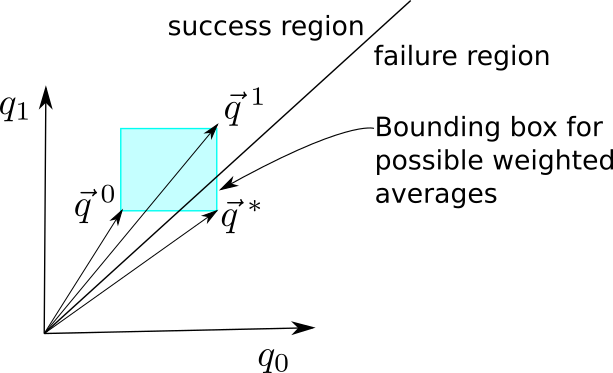
\includegraphics[width=3.5in]
{simpson/q-vecs.png}
\caption{$\vec{q}^{\;0}$,
$\vec{q}^{\;1}$ vectors
and bounding box for vector $\vec{q}^{\;*}$.  } 
\label{fig-simpson-q-vecs}
\end{figure}

It is possible (see Fig.\ref{fig-simpson-q-vecs} 
for a graphical explanation of how)
 to find perverse cases in which
 $ P(a=1|t, g=0)$ and $ P(a=1|t, g=1)$
 increase with $ t$ but $ P(a=1|t)$ 
decreases with $ t$. So it is possible 
to conclude that the medicine is a failure
 for each of the two $ g$ populations 
considered separately, yet the medicine 
is a success when both populations are 
``amalgamated". The lesson is that a
 ``trend reversal" is possible 
upon amalgamation. Trends
are not necessarily preserved 
when we do a weighted average of
 type $ E_{\ul{g}|t}$. 
$ E_{\ul{g}|t}$ is an expected value
 on the random variable $ \ul{g}$
 conditioned on the root 
random variable $ \ul{t}$.


So far, we have proven that probabilistically, 
the drug can be a failure for the populations
 of both sexes considered separately, 
but a success for the aggregate population.

\section*{Pearl Causality}

Pearl Causality would add 
the following two 
important insights 
to this problem:
\begin{enumerate}
\item bnets Fig.\ref{fig-simpson-chain} 
and Fig.\ref{fig-simpson-fork}, 
although they are
probabilistically equivalent, 
do not represent the same physical
 situation. In fact, only
 Fig.\ref{fig-simpson-fork} 
occurs in this case.
\item To decide whether the
 medicine is effective, we 
must apply a $do()$ operator to
 the $ t$ variable in
 Fig.\ref{fig-simpson-fork}. 
The effect of that $do()$ operator
 is to erase the arrow going 
from $ g$ to $ t$. This in turn means
 that the average $ E_{\ul{g}|t}$
 in our equation for $ P(a=1|t)$
 becomes a simpler average $ E_{\ul{g}}$
 which is independent of $ t$. 
But for such an average,
 the
 bounding box in Fig.\ref{fig-simpson-q-vecs}
 degenerates to its diagonal 
line that connects the tips
 of the two vectors $ \vec{q}^{\;0}$
 and $ \vec{q}^{\;1}$. The vector 
$ \vec{q}^{\;*}$ must now fall on 
that diagonal line and must therefore
 also fall in the success region.
\end{enumerate}
In conclusion, as Judea Pearl would say,
 if we ask the right question to Nature,
 i.e., what is
 $ P[a=1 | do(\ul{t}=t)]$ for $ t=0,1$,
 we get as an answer that the 
aggregate population preserves 
rather than reverses the
 unanimous trend of the 
two gendered populations.
\newpage
\section*{Numerical Example}

\begin{table}[h!]
\centering
\begin{tabular}{|l|l|l|}
\hline
\rowcolor[HTML]{ECF4FF} 
(a,t,g) & \begin{tabular}[c]{@{}l@{}}number of patients\\ separated by gender\end{tabular} & \begin{tabular}[c]{@{}l@{}}number of patients\\ of either gender\end{tabular} \\ \hline
0,0,0 & 19 & 47 \\ \cline{1-2}
0,0,1 & 28 &  \\ \hline
0,1,0 & 37 & 49 \\ \cline{1-2}
0,1,1 & 12 &  \\ \hline
1,0,0 & 1 & 13 \\ \cline{1-2}
1,0,1 & 12 &  \\ \hline
1,1,0 & 3 & 11 \\ \cline{1-2}
1,1,1 & 8 &  \\ \hline
\end{tabular}
\caption{Data for numerical example 
 of Simpson's Paradox. This 
fictitious data was taken directly
 from Table 6.4, page 210
of ``The Book of Why", 
Ref.\cite{book-why}.}
\label{tab-simpson-heat-attack}
\end{table}

\beq
P(a|t,g)=
\begin{array}{c|cccc}
&\scriptstyle 0,0 & \scriptstyle 0,1 &
\scriptstyle  1,0 &\scriptstyle 1,1\\\hline
\scriptstyle  0& 19/20 & 28/40 & 37/40 & 12/20\\
\scriptstyle 1& 1/20 & 12/40 & 3/40 & 8/20
\end{array}
\eeq

\beq
P(a|t)=
\begin{array}{c|cc}
&\scriptstyle 0 & \scriptstyle 1\\\hline
\scriptstyle 0& 47/60& 49/60\\
\scriptstyle  1& 13/60 & 11/60
\end{array}
\eeq

\beq
\begin{array}{lll}
\frac{
P(a=1,t=1, g=0)
}{
\sum_aP(a, t=1, g=0)
}=
P(a=1|t=1, g=0) &=& \frac{3}{40}
\\
\frac{
P(a=1,t=0, g=0)
}{
\sum_aP(a, t=0, g=0)
}=
P(a=1|t=0, g=0) &=& \frac{1}{20}=\frac{2}{40}
\end{array}
\label{eq-g-eq-0}
\eeq

\beq
\begin{array}{lll}
\frac{
P(a=1,t=1, g=1)
}{
\sum_aP(a, t=1, g=1)
}=
P(a=1|t=1, g=1) &=& \frac{8}{20}=\frac{16}{40}
\\
\frac{
P(a=1,t=0, g=1)
}{
\sum_aP(a, t=0, g=1)
}=
P(a=1|t=0, g=1) &=& \frac{12}{40}
\end{array}
\label{eq-g-eq-1}
\eeq

\beq
\begin{array}{lll}
\frac{
\sum_g P(a=1,t=1, g)
}{
\sum_g\sum_aP(a, t=1, g)
}=
P(a=1|t=1) &=& \frac{11}{60}
\\
\frac{
\sum_g P(a=1,t=0, g)
}{
\sum_g\sum_aP(a, t=0, g)
}=
P(a=1|t=0) &=& \frac{13}{60}
\end{array}
\label{eq-g-eq-all}
\eeq

Note
that the right hand
side
of 
Eq.\ref{eq-g-eq-0}
is higher
for $t=1$
than for $t=0$.
Same trend 
occurs
in Eqs.\ref{eq-g-eq-1}
but
is reversed in Eqs.\ref{eq-g-eq-all}.
\chapter{Structure and Parameter
 Learning for Bnets}\label{ch-struc-learn}


Learning a bnet
from data
is a computationally intensive NP-complete
problem. 
Therefore,
the best one can hope
for is for heuristic algorithms 
that solve this problem
approximately. A huge number 
of such algorithms have been tried
and continue to be tried.
Luckily,
there exists a free open source
 software library
called \bnlearn
that covers many of
them. The goal
of this chapter
is to give
a brief
overview
of the subject
of bnet 
learning,
after 
which
we recommend
to
those readers who
want to
pursue this subject
further,
to 
learn \bnlearn.

This chapter
is based on  
the \bnlearn website Ref.\cite{bnlearn}, and
on a 2019 survey
paper 
\cite{scutari2019}
by Scutari et al.
I highly recommend looking
at both. Refs.
\cite{carvalho} and \cite{margaritis}
were also
helpful to me in understanding this subject.

\bnlearn (Ref.\cite{bnlearn})
(free, open source) is 
very
comprehensive
and well
maintained. It
is 
written 
mostly in C with
an R front-end.
It was
developed by Marco Scutari
and collaborators
over a time period of
more than 10 years,
and is still
under active development.
How things stand
in the field of
bnet learning software reminds me
of how things stand in 
the field of linear 
algebra (LA) software. Perfecting and
optimizing
LA software
takes many years, so
I would not
advise you to write your own
LA software library starting
from scratch.
There is no need to do so. Instead, you
can use LAPACK (free, open source), which
has been perfected and expanded
for decades by world experts. 
I view \bnlearn as the LAPACK
of bnet learning. 



\section{Overview}

To give
the reader an overview
of the subject
and of \bnlearn itself,
here is a highly
simplified tree,
compiled from
the \bnlearn website
and documentation,
of some of the
subjects covered by \bnlearn.



\dirtree{%
.1 Parameter Learning.
.2 missing data.
.1 Structure Learning.
.2 tree-like structures given a priori.
.3 Naive Bayes.
.3 Chow-Liu tree.
.3 Tree Augmented Naive Bayes (TAN).
.3 ARACNE.
.2 score based.
.3 algorithms.
.4 hill climbing (HC).
.4 HC with random restarts.
.4 HC with Tabu list (Tabu).
.4 simulated annealing.
.4 genetic algorithms.
.3 scoring functions.
.4 Information Theoretic scores.
.4 Bayesian Information Criterion (BIC).
.4 Bayesian Dirichlet (BD) family.
.2 constraint based.
.3 algorithms.
.4 PC family.
.4 Grow-Shrink (GS).
.4 Incremental Association Markov Blanket (IAMB) family.
.3 conditional independence tests.
.4 mutual information (parametric, semiparametric and permutation tests).
.4 shrinkage-estimate for the mutual information.
.2 hybrid.
.3 Max-Min Hill Climbing (MMHC).
.3 Hybrid HPC (H2PC).
.3 General 2-Phase Restricted Maximization (RSMAX2).
.1 parallel mode structure learning.
.1 node types.
.2 all-discrete.
.2 all-continuous.
.2 mixed.
.1 utility functions.
.2 model comparison and manipulation.
.2 random data generation.
.2 arc orientation testing.
.2 simple and advanced plots.
.2 parameter estimation (maximum likelihood 
and Bayesian).
.2 inference, conditional probability queries. 
.2 cross-validation.
.2 bootstrap.
.2 model averaging.
}
     

\hrule
Let
\begin{itemize}
\item
PL=parameters learning (i.e, 
learning the TPMs)
\item
SL= structure learning 
(i.e., learning the DAG)
\item
ML= model (or bnet) learning, SL+PL
\end{itemize}

PL is easy, once the
structure is known. PL 
assuming no missing data
goes as follows.
Using the notation of Chapter 
\ref{ch-scoring}, define
\beq
\pi_\kbarmu^i=
P(\rvx_i=k\cond pa(\rvx_i)=\mu )
\;.
\eeq
Then $\pi_\kbarmu^i$
can be estimated
from the data $N^i_\kmu$ 
using:

\beq
\pi_\kbarmu^i
\approx 
N^i_\kbarmu
=
\frac{N^i_\kmu}{N^i_\plusmu}
\;.
\label{eq-PL-simple}
\eeq
PL
described by Eq.(\ref{eq-PL-simple})
 is only for discrete nodes
with no missing data.
\bnlearn  can also do PL
with missing data
and continuous 
(Gaussian linear only) nodes. 
See Chapter \ref{ch-missing-d}
on missing data
and Chapter \ref{ch-gauss-lin}
on Gaussian linear nodes.
SL
actually
does PL and SL
at the same time. 
 
There are 3 main 
types of SL: score based,
constraint based, and hybrid.
\bnlearn 
 can perform many
 algorithms
of each of these 3 types
of SL.
It can perform
most of them with either all-discrete,
or all-continuous
or mixed nodes.
It can perform
many of them
in parallel mode.
The 2019 survey paper
Ref.\cite{scutari2019} by
Scutari et al
compares 
the performance 
of many different
bnet learning algorithms.

\section{Score based SL algorithms}

Score based SL algorithms
require
scoring bnets (with either
all-discrete, all-continuous
or mixed nodes).
See Chapter \ref{ch-scoring}
for an introduction
to scoring bnets.
The BIC score
explained
in that chapter is
very popular
and works for all-discrete,
all-continuous or mixed nodes.

Score-based SL algorithms apply
standard
optimization techniques. 
In the Hill Climbing algorithm,
the current best
bnet is changed
slightly
and then given a score
that measures how well
it fits the data.
The bnet with the highest (=best) 
score so far, as well as that highest score,
are stored. (Hence,
this is called a greedy search).
The process continues
until the latest highest score stops changing.
The problem with being
greedy all the time is that
the answer might
converge to a local maximum.
To mitigate
this problem
and allow some
probability of visiting more
than one
local maximum, one uses a
Tabu Table, random restarts,
simulated annealing, genetic algorithms,
etc.

\section{Constraint based SL algorithms}

To fully understand
 constraint based SL 
algorithms,
the reader 
is advised to read Chapters 
\ref{ch-dsep} and \ref{ch-obs-equi}
first.

Constraint based SL algorithms
require
estimating from the data
the conditional independence
$\rvx.\perp_P \rvy.|\rva.$ 
for any 3 disjoint
multinodes $\rvx., \rvy., \rva.$.
This can be done by
estimating the conditional
mutual information (CMI)
$H(\rvx.:\rvy.|\rva.)$.
\bnlearn  can calculate CMI and
other metrics
of $\rvx.\perp_P \rvy.|\rva.$.
All these metrics are very
similar; they 
all measure
how close
$P(x.|y., a.)$
and $P(x.|a.)$ are.

The first
constraint-based SL algorithm
was the Inductive Causation (IC) algorithm
 proposed by Pearl and Verma in 1991.
Incremental
improvements
have been
proposed since then, such as
the PC family
of algorithms,
Grow-Shrink and
the
Incremental Association Markov Blanket (IAMB)
family of algorithms.

\newpage
\section{Pseudocode
for some bnet learning algorithms}






\begin{algorithm}
	\DontPrintSemicolon
    \SetKwInOut{KwIn}{Input}
    \SetKwInOut{KwOut}{Output}

    \KwIn{Data $D$, Vertices $V$}
    \KwOut{a bnet $B=(G, T)$,
	where $G=(V, E)$ is a DAG, where
	$V$ are its vertices (nodes) and $E$ 
	are its edges (arrows).
 	$T$ are all its
	Transition Probability Matrices (TPMs)
 	$T=TPMs(G, D)$. }

    $E\larrow \emptyset$\;
	$T\larrow \emptyset$\;
	$B\larrow (V, E, T)$\;
	$maxscore \larrow-\infty$\;
	\tcp{$DE$= all possible directed edges}
	$DE=\{\rvx\rarrow\rvy\in V\times V: \rvx\neq \rvy\}$\;
	$again\larrow True$\;
	\While{$again$}{
		\For{all $\rvx\rarrow\rvy\in DE$}{
			\tcp{add arrow}
			$E_+\larrow E\cup\{\rvx\rarrow\rvy\}$\;
			\tcp{delete arrow}
			$E_-\larrow E-\{\rvx\rarrow\rvy\}$\;
			\tcp{reverse arrow}
			$E_R\larrow E_-\cup\{\rvy\rarrow\rvx\}$\;
			\For{$E'=E_+,E_-, E_R$}{
				\If{$E'\neq E$ and $G'=(V, E')$ is a legal DAG}{
					$T'\larrow TPMs(G', D)$\;
					$B'\larrow (G', T')$\;
					$newscore= \text{BIC-score}(B')$\;
					\eIf{$newscore>maxscore$}{
						$B\larrow B'$\;
						$maxscore\larrow newscore$\;
					}{
						$again\larrow False$
					}
				}
			}
		}
	}
    \KwRet{$B$}
    \caption{Pseudocode for Hill Climbing algorithm}
\end{algorithm}



\begin{algorithm}
	\DontPrintSemicolon
    \SetKwInOut{KwIn}{Input}
    \SetKwInOut{KwOut}{Output}

    \KwIn{Data $D$, Vertices (nodes) $V$,
	tolerance in CMI $\eps>0$}
    \KwOut{partially oriented
	acyclic graph $G=(V, E, UE)$, where $V$ are 
	the vertices (nodes),
	$E$ are the oriented edges (arrows)
	and $UE$ are the unoriented edges.}
	$E\larrow \emptyset$\;
	\tcp{initialize $UE$ to fully-connected
	undirected graph} 
	$UE\larrow \{\rvx-\rvy\in V\times V: \rvx-\rvy=\rvy-\rvx,
	\rvx\neq \rvy\}$\;
	\tcp{Shrink phase. Deletes edges from $E$.}
	\For{$\lam=0, 1, 2, \ldots, |V|-2$}{
		\For{all $\rvx-\rvy\in UE$}{
			\For{all $S=\{\rva\in V:\rvx-\rva\in UE, 
			\rva\neq \rvx, \rvy\} \ni |S|=\lam$}{
				\If{$H(\rvx:\rvy|S)<\eps$}{
					\tcc{If there were an arrow between $\rvx$ and $\rvy$, 
						then conditioning on $S$ would not be enough
						to interrupt info transmission $H(\rvx:\rvy|S)$
						 between $\rvx$ and $\rvy$}
					$UE\larrow UE-\{\rvx-\rvy\}$\;
					$S(\rvx-\rvy)\larrow S$\;
				}
			}
		}
	}
	\tcp{Growth phase. Adds v structures to $E$.}
	\For{all $\rvx,\rvy, \rva$ such that
	$\rvx-\rva\in UE, \rva-\rvy\in UE,
	\rvx-\rvy\not \in UE, \rva\not\in S(\rvx-\rvy)$}{
		\tcc{If there were no collider at $\rva$, then 
		there would be info transmission  between $\rvx$ and
		$\rvy$}
		$UE\larrow UE-\{\rvx-\rva, \rva-\rvy\}$\;
		$E\larrow E\cup \{\rvx\rarrow\rva, \rvy\rarrow\rva\}$\;
	}
	\tcp{Orienting edges.}
	$again\larrow True$\;
	$size\larrow |UE|$\;
	\While{$again$}{
		\For{all $\rvx-\rvy\in UE$}{
			\If{$\rvx\rarrow\rvy\in E$,
			$\rvy-\rvz\in UE$,
			$\rvx-\rvz\not\in UE$,
			$\not\exists \rvw \ni \rvw\rarrow\rvy\in E$}{
				\tcp{to avoid introducing new v structure}
				$UE\larrow UE- \{\rvy-\rvz\}$\;
				$E\larrow E\cup \{\rvy\rarrow \rvz\}$\;
			}
			\If{$\rvx\rarrow\rvy\in E$
			and there is directed path from $\rvx$ to
			$\rvy$ in $E$}{
				\tcp{to avoid introducing cycles}
				$UE\larrow UE- \{\rvx-\rvy\}$\;
				$E\larrow E\cup \{\rvx\rarrow \rvy\}$\;
			}
		}
		$newsize\larrow |UE|$\;
		\eIf{$size==newsize$}{
			$again\larrow False$\;
		}{
			$size\larrow newsize$\;
		}
	}
    \KwRet{$G=(V, E, UE)$}
    \caption{Pseudocode for PC-Stable algorithm}
\end{algorithm}
\chapter{\;\;Turbo Codes}
This chapter is based
 on Ref.\cite{mackay98}.

In this chapter, vectors
with $n$ components
will be indicated by 
an $n$ superscript. For example,
$a^n=(a_0, a_1, \ldots, a_{n-1})$.



Consider
an  n-letter message $u^n=
(u_0, u_1, \dots, u_{n-1})$,
where for all $i$,
$u_i\in \cala$ is an element of
an alphabet $\cala$,
and where 
for all $i$, the $\rvu_i$ are i.i.d..
Suppose $u^n$
is encoded 
deterministically in
two different ways, $e_1(u^n)$
and $e_2(u^n)$.
After passing through 
the same memoryless channel, the variables
$u^n,e_1, e_2$
become $\tilu^n, \tile_1,
\tile_2$, respectively.
The letter $u$ stands 
for unencoded, and $e$ for
encoded. Quantities with a tilde
$\tilu^n, \tile_1,
\tile_2$
occur after channel passage
and are visible (measurable). Quantities
without a tilde
$u^n, e_1,
e_2$ are hidden (unmeasurable).


The situation just described
can be represented by
the bnet Fig.\ref{fig-turbo-ext},
or by its abridged version
Fig.\ref{fig-turbo-simple}.
But note that the abridged version does not
show explicitly that the
$u_i$ are i.i.d. or that the 
 channel is memoryless (i.e., that
the $u_i$ for all $i$
pass independently
through the channel).

\begin{figure}[h!]
\centering
$$\xymatrix{
\rvu_0\ar[rr]\ar[rddd]\ar[rdddd]
&&\tilu_0\\
\rvu_1\ar[rr]\ar[rdd]\ar[rddd]
&&\tilu_1\\
\rvu_2\ar[rr]\ar[rd]\ar[rdd]
&&\tilu_2\\
&\rve_1\ar[r]&\tile_1\\
&\rve_2\ar[r]&\tile_2
}$$
\caption{Turbo coding Bnet
representing a message
being 
encoded two
different ways 
and then the
original 
message and the 2
encodings
pass through a memoryless channel.
}
\label{fig-turbo-ext}
\end{figure}

\begin{figure}[h!]
\centering
$$\xymatrix{
\rvu^n\ar[rr]\ar[rd]\ar[rdd]
&&\tilu^n\\
&\rve_1\ar[r]&\tile_1\\
&\rve_2\ar[r]&\tile_2
}$$
\caption{Abridged version of Fig.\ref
{fig-turbo-ext}.}
\label{fig-turbo-simple}
\end{figure}

Define 


\beq
x=(u^n, e_1, e_2)
\eeq
and

\beq
\tilx=(
\tilu^n,
\tile_1, 
\tile_2)
\;.
\eeq

Fig.\ref{fig-turbo-ext} 
implies that

\beq
P(x, \tilx)
=
P(\tilu^n|u^n)\left[\prod_{r=1,2}
 P(\tile_r|e_r)
P(e_r|u^n)\right]
P(u^n)
\;.
\eeq
Because the $u^n$ are i.i.d.,

\beq\color{blue}
P(u^n)=
\prod_i P(u_i)
\;.
\eeq
Because the channel is memoryless, 

\beq\color{blue}
P(\tilu^n|u^n)=\prod_i P(\tilu_i|u_i)
\;.
\eeq
Because the encoding
is deterministic, we must have
for  $r=1,2$
\beq\color{blue}
P(e_r|u^n)=\delta(e_r, e_r(u^n))
\;.
\eeq

Define the belief functions

\beq
BEL_i=BEL_i(\rvu_i=a)=P(\rvu_i=a|\tilx)
\;.
\eeq
The best estimate of $u_j$
given all visible evidence $\tilx$
is

\beq
\HAT{u}_i=
\argmax_{u_i}BEL_i(u_i)
\;.
\eeq


Define the probability functions
\beq
\pi_i=\pi_i(u_i)=P(u_i)
\;,
\eeq
and the likelihood functions

\beq
\lam_i=\lam_i(u_i)=P(\tilu_i|u_i)
\;.
\eeq

For $r=1,2$, define the Kernel functions

\beq
K_r=K_r(u^n)=
P(\tile_r|e_r=e_r(u^n))
\;.
\eeq

In this book,
$\caln(!a)$ denotes
a normalization constant 
that does not depend
on $a$. Define
\beq
\caln_i=\caln(!u_i)
\;.
\eeq

\begin{claim}
\beq
BEL_i=\caln_i\lam_i\pi_i
\calt_i^{K_1K_2}
[\prod_{j\neq i} \lam_j\pi_j]
\label{eq-bel-exact}
\;,
\eeq
where $\calt^K_i(\cdot)$ with $K=K_1K_2$
is an operator (transform)
that acts on functions of $u^n$:

\beq
\calt_i^K(\cdot)=
\sum_{u^n}\delta(u_i,a)K(u^n)(\cdot)
\;.
\eeq

\end{claim}
\proof

\beqa
\lefteqn{P(\rvu_i=a|\tilx) =}\nonumber\\
&=&\sum_{x}\delta(u_i, a)P(x|\tilx)\\
&=&\sum_{x}\delta(u_i, a)
\frac{P(\tilx|x)P(x)}{P(\tilx)}\\
&=&\caln(!a)
\sum_{x}\delta(u_i, a)
P(\tilx|x)P(x)\\
&=&
\caln(!a)
\sum_{x}\delta(u_i, a)P(u^n)
\left[
\prod_{r=1,2}
P(\tile_r|e_r)\delta(e_r,e_r(u^n))
\right]
\prod_j P(\tilu_j|u_j)\\
&=&\caln(!a)
\lam_i(a)\pi_i(a) R
\;, 
\eeqa
where

\beqa
R&=&
\sum_{u^n}\delta(u_i, a)
\left[
\prod_{r=1,2}
P(\tile_r|e_r(u^n))\right]
\prod_{j\neq i} P(\tilu_j|u_j)P(u_j)\\
&=&
\sum_{u^n}\delta(u_i, a)
\left[
\prod_{r=1,2}
K_r(u^n)\right]
\prod_{j\neq i} \lam_j(u_j)\pi_j(u_j)\\
&=&\calt_i^{K_1K_2}
[\prod_{j\neq i} \lam_j(u_j)\pi_j(u_j)]
\;.
\eeqa
Hence

\beq
BEL_i(a)=\caln(!a)\lam_i(a)\pi_i(a)
\calt_i^{K_1K_2}
[\prod_{j\neq i} \lam_j(u_j)\pi_j(u_j)]
\;.
\eeq
\qed


\section{Decoding Algorithm}
The Turbo algorithm for
decoding the encode message
 is as follows.
For $m=0$, let

\beq
\pi_j^{(0)}(u_j) = \frac{1}{n_{\rvu_j}}
\;.
\eeq
Then for $m=1, 2, \dots $, let

\beq
\pi_i^{(m)}=\caln_i
\calt_i^{K_{m\%2}}
[\prod_{j\neq i} \lam_j\pi_j^{(m-1)}]
\;,
\eeq
 where $m\%2=1$ if $m$ is odd and 
$m\%2=2$ if $m$ is even. 
Furthermore, for $m>0$, let

\beqa
BEL_i^{(m)}&=&\caln_i \lam_i
\pi_i^{(m-1)}\pi_i^{(m)}
\\
&=&
\caln_i\lam_i \pi_i^{(m-1)}\calt_i^{K_{m\%2}}
[\prod_{j\neq i} \lam_j
\pi_j^{(m-1)}]
\;.
\label{eq-bel-approx}
\eeqa
As $m\rarrow\infty$, 
$BEL_i^{(m)}$ given 
by Eq.(\ref{eq-bel-approx}) is
 expected to 
converge to the the exact 
$BEL_i$ given
by Eq.(\ref{eq-bel-exact}).

Turbo decoding 
can be represented by the bnets 
Figs.\ref{fig-turbo-decode}
and \ref{fig-turbo-decode-ext}.


\begin{figure}[h!]
\centering
$$\xymatrix{
\ul{\tilu}^n
\ar[r]
\ar@/^1pc/[rr]
\ar@/^1pc/[rrr]
\ar@/^1pc/[rrrr]
\ar@/^1pc/[rrrrr]
&\rvd_i^{(1)}
&\rvd_i^{(2)}
&\rvd_i^{3)}
&\rvd_i^{(4)}
&\rvd_i^{(5)}
\\
\ul{\tile}_1
\ar[ur]\ar[urrr]\ar[urrrrr]\\
\ul{\tile}_2
\ar[uurr]\ar[uurrrr]
}$$
\caption{Bnet
describing Turbo code
generation of $BEL_i^{(m)}(a)$
for $m=1,2, \ldots$.}
\label{fig-turbo-decode}
\end{figure}

\begin{figure}[h!]
\centering
$$\xymatrix{
&
&\ul{BEL}^{n(1)}(\cdot)
&\ul{BEL}^{n(2)}(\cdot)
&\ul{BEL}^{n(3)}(\cdot)
&\ul{BEL}^{n(4)}(\cdot)
\\
\rvu^n
&\ul{\pi}^{n(0)}(\cdot)\ar[r]\ar[ur]
&\ul{\pi}^{n(1)}(\cdot)\ar[r]\ar[u]\ar[ur]
&\ul{\pi}^{n(2)}(\cdot)\ar[r]\ar[u]\ar[ur]
&\ul{\pi}^{n(3)}(\cdot)\ar[r]\ar[u]\ar[ur]
&\ul{\pi}^{n(4)}(\cdot)\ar[u]
\\
\ul{\tile}_1\ar[urr]\ar[urrrr]\\
\ul{\tile}_2\ar[uur]\ar[uurrr]\ar[uurrrrr]
\\
\ul{\tilu}^n\ar[r]
&\ul{\lam}^{n}(\cdot)
}$$
\caption{
Bnet
describing Turbo code
generation of $BEL^{n(m)}(\cdot)$ and
$\pi^{n(m)}(\cdot)$ 
for $m=0,1,2 \ldots$.
The following arrows 
were not drawn
for clarity:
Arrows pointing from node
 $\ul{\lam}^n(\cdot)$ to nodes 
$\ul{\pi}^{n(m)}(\cdot)$ 
and $\ul{BEL}^{n(m)}(\cdot)$ for 
$m=0,1,2, 
\ldots$.
}
\label{fig-turbo-decode-ext}
\end{figure}

The TPMs, printed in blue,
for bnet Fig.\ref{fig-turbo-decode},
are as follows.


\beq\color{blue}
P(d_i^{(m)}=a\cond
\tilu^n, \tile_{m\%2})=BEL^{(m)}_i(a)
\;.
\eeq

The TPMs, printed in blue,
for bnet Fig.\ref{fig-turbo-decode-ext},
are as follows.



\beq\color{blue}
P((\lam^n)'(\cdot)|\tilu^n)=
\delta((\lam^n)'(\cdot),
 \lam^n(\cdot))
\eeq

\beq\color{blue}
P(\pi^{n(m)}(\cdot)|\lam^n(\cdot), 
\pi^{n(m-1)}(\cdot), \tile_{m\%2})=
\prod_i\prod_{u_i}
\delta(\pi_i^{(m)}(u_i),
\caln_i
\calt_i^{K_{m\%2}}
[\prod_{j\neq i} \lam_j\pi_j^{(m-1)}])
\eeq

\beq\color{blue}
P(BEl^{n(m)}(\cdot)|\lam^n(\cdot),
\pi^{n(m)}(\cdot),
\pi^{n(m-1)}(\cdot))=
\prod_i\prod_{u_i}
\delta(
BEL_i(u_i),
\caln_i \lam_i
\pi_i^{(m-1)}\pi_i^{(m)})
\eeq


\section{Message Passing 
Interpretation of Decoding Algorithm}

Ref.\cite{mackay98} shows that
the  Turbo code
decoding algo can be
interpreted
as an 
application of Message Passing.
We leave all talk of Message Passing to
a separate
chapter, Chapter \ref{ch-mpass}.
\chapter{Variational Bayesian Approximation}

For more info and references about
this topic, see Ref.\cite{wiki-var-bay}.

The Variational Bayesian approximation (VBA)
is an analytic 
(as opposed to numerical) approximation
to the probability 
distribution $P(h|\vecx)$,
where $h$ are the hidden variables 
and $\vecx$ is the data. 


More precisely, suppose $\rvh\in S_\rvh$ and $\rvq\in S_\rvh$.
Suppose $\vec{\rvx}\in S_\rvx^{nsam}$
 is a vector of $nsam$ samples
and the samples $\rvx[\sigma]\in S_\rvx$ are i.i.d..
 The VBA is simply 
an approximation
$P_{\rvq|\vec{\rvx}}$ to
$P_{\rvh|\vec{\rvx}}$:


\beq
P_{\rvh|\vec{\rvx}}(h|\vecx)
\approx P_{\rvq|\vec{\rvx}}(h|\vecx)
\eeq
obtained by minimizing the Kullback-Liebler divergence
$D_{KL}(P_{\rvq|\vec{\rvx}}\parallel
P_{\rvh|\vec{\rvx}})$
over all 
$P_{\rvq|\vec{\rvx}}$. The minimization
is 
usually subject to some constraints
on the admissible forms of 
$P_{\rvq|\vec{\rvx}}$.


$D_{KL}(Q\parallel P)\neq
D_{KL}(P\parallel Q)$; i.e.,  $D_{KL}$ is not
symmetric. So why do we use 
$D_{KL}(P_{\rvq|\vec{\rvx}}\parallel
P_{\rvh|\vec{\rvx}})$
instead of 
$D_{KL}(
P_{\rvh|\vec{\rvx}}\parallel P_{\rvq|\vec{\rvx}})$?
Because 
$D_{KL}(
P_{\rvh|\vec{\rvx}}\parallel P_{\rvq|\vec{\rvx}})$
requires knowledge of $P_{\rvh|\vec{\rvx}}$,
but calculating $P_{\rvh|\vec{\rvx}}$
is what we are trying to do in the first place.

\begin{figure}[h!]
\centering
\includegraphics[width=2.5in]
{var-bay/kl-q-support.png}
\caption{
If $P_\rvq(h)$
is Gaussian shaped 
and $P_\rvh(h)$
has multiple
bumps (modes)
then 
$D_{KL}(P_\rvq\parallel P_\rvh)$
is minimized when $P_\rvq$
fits one of the modes of $P_\rvh$.
That is because $D_{KL}(P_\rvq\parallel P_\rvh)=
\sum_h P_\rvq(h)\ln \frac{P_\rvq(h)}{P_\rvh(h)}$
is a weighted average with weights $P_\rvq$,
so nothing going on outside the support
of $P_\rvq$ influences  much
the final average.
}
\label{fig-kl-q-support}
\end{figure}


See Fig.\ref{fig-kl-q-support}
for some intuition
on what minimizing
$D_{KL}(P_{\rvq|\vec{\rvx}}\parallel
P_{\rvh|\vec{\rvx}})$ means.


\begin{figure}[h!]
$$\xymatrix{
& \rvh_0\ar[r]
& \rvh_1
\\
\rvx[0]
\ar[ru]\ar[rru]
\ar[rddd]\ar[rrddd]
\\
\rvx[1]
\ar[ruu]\ar[rruu]
\ar[rdd]\ar[rrdd]
\\
\rvx[2]
\ar[ruuu]\ar[rruuu]
\ar[rd]\ar[rrd]
\\
&
\rvq_0
&
\rvq_1
}$$
\caption{
$\rvq$ 
and $\rvh$ have  $nh=2$
mirroring components and
those of $\rvq$ are independent
at fixed $\vec{\rvx}$.}
\label{fig-q-apes-h}
\end{figure}


Suppose $\rvh=(\rvh_0, \rvh_1, \ldots, \rvh_{nh-1})$
and
$\rvq=(\rvq_0, \rvq_1, \ldots, \rvq_{nh-1})$
where $\rvh_i\in S_{\rvh_i}$
and $\rvq_i\in S_{\rvh_i}$ for all $i$.
We say $\rvq$ 
and $\rvh$ have  $nh$ mirroring
 components and
those of $\rvq$ are independent
at fixed $\vec{\rvx}$ if

\beq
P_{\rvq|\vec{\rvx}}(h|\vecx)
=\prod_i P_{\rvq_i|\vec{\rvx}}(h_i|\vecx)
\;.
\eeq
The bnet Fig.\ref{fig-q-apes-h}
describes the scenario that
we have in mind: The samples 
$\rvx[\sigma]$ are i.i.d..
Each component $\rvh_i$
of $\rvh$ has a 
mirroring
component $\rvq_i$
in $\rvq$.
The components of
$\rvh$ are correlated
whereas those of $\rvq$
are independent
at fixed $\vec{\rvx}$.

\begin{claim}
If $\rvq$
and $\rvh$ 
 have $nh$ mirroring components 
and those of $\rvq$ are independent
at fixed $\vec{\rvx}$ and
$D_{KL}(P_{\rvq|\vec{\rvx}}\parallel
P_{\rvh|\vec{\rvx}})$
is minimum
 over all $P_{\rvq|\vec{\rvx}}$, then

\beqa
P_{\rvq_i|\vec{\rvx}}(q_i|\vecx)
&=&
\caln(!q_i)
e^{
E_{(\rvq_j)_{j\neq i}}[
\ln P_{\rvh| \vec{\rvx}}(\rvh=q|\vecx)]
}
\label{eq-fixed-vecx}
\\
&=&
\caln(!q_i)
e^{
E_{(\rvq_j)_{j\neq i}}[
\ln P_{\rvh, \vec{\rvx}}(\rvh=q, \vecx)]}
\;
\eeqa
for all $i$.
\end{claim}
\proof

Since all quantities in Eq.(\ref{eq-fixed-vecx})
are conditioned on $\vecx$, let 
us omit all mention of 
$\vecx$ in this proof.

Let

\beq
\call= \call_0 + \call_1
\eeq
where

\beqa
\call_0
&=&
D_{KL}(P_{\rvq}\parallel P_{\rvh})
\\
&=&
\sum_h P_\rvq(h)\ln \frac{P_\rvq(h)}{P_\rvh(h)}
\\
&=&
\sum_h P_{\rvq}(h)\ln P_\rvq(h)
- \sum_h P_{\rvq}(h)\ln P_\rvh(h)
\\
&=&
\sum_i \sum_{h_i}
 P_{\rvq_i}(h_i)\ln P_{\rvq_i}(h_i)
- \sum_h P_{\rvq}(h)\ln P_\rvh(h)
\eeqa
and

\beq
\call_1=
\sum_i \lam_i \left[
\sum_{h_i}P_{\rvq_i}(h_i)-1\right]
\;.
\eeq
Then   

\beq
\delta \call=
\sum_i
\sum_{h_i}
\delta P_{\rvq_i}(h_i)
\left[
\ln P_{\rvq_i}(h_i)
+1 + \lam_i
-\;\frac{1}{nh}\sum_{(h_j)_{j\neq i}}
\prod_{(h_j)_{j\neq i}}
\{P_{\rvq_j}(h_j)\}\ln P_\rvh(h)
\right]
\;.
\eeq
Hence,

\beq
P_{\rvq_i}(h_i)
=
\caln(!h_i)
e^{
\sum_{(h_j)_{j\neq i}}
\left\{\prod_{(h_j)_{j\neq i}}
P_{\rvq_j}(h_j)\right\}\ln P_\rvh(h)
}
\;.
\eeq
\qed

Note that 
Eq.(\ref{eq-fixed-vecx})
yields
a  system
of $nh$ nonlinear equations
in $nh$ unknowns
$(P_{\rvq_i|\vec{\rvx}})_
{i=0, 1, \dots, nh-1}$.
This system 
is usually solved recursively.


\section{Free Energy $\calf(\vecx)$}

To simplify the notation
below, let us
introduce
the following
abbreviations:

\beq
P(h|\vecx)=P_{\rvh|\vec{\rvx}}(h| \vecx)
\eeq

\beq
P(h,\vecx)=P_{\rvh,\vec{\rvx}}(h, \vecx)
\eeq

\beq
P(\vecx)=P_{\vec{\rvx}}(\vecx)
\eeq

Note that

\beqa
D_{KL}(P_{\rvq|\vec{\rvx}}\parallel
P_{\rvh|\vec{\rvx}})&=&
\sum_h P_{\rvq|\vec{\rvx}}(h|\vecx)\ln
 \frac{P_{\rvq|\vec{\rvx}}(h|\vecx)}{P(h|\vecx)}
\\
&=& \sum_h P_{\rvq|\vec{\rvx}}(h|\vecx)\ln
 \frac{P_{\rvq|\vec{\rvx}}(h|\vecx)}{P(h,\vecx)}
+ \ln P(\vecx)
\\
&=&
\calf(\vecx)+ \ln P(\vecx)
\eeqa
Hence, the {\bf Free energy} $\calf(\vecx)$
 is defined as

\beqa
\calf(\vecx)&=&
\sum_h P_{\rvq|\vec{\rvx}}(h|\vecx)\ln
 \frac{P_{\rvq|\vec{\rvx}}(h|\vecx)}{P(h,\vecx)}
\\
&=&
E_{\rvq|\vec{\rvx}}\left[
\ln
 \frac
{P_{\rvq|\vec{\rvx}}(q|\vecx)}
{P_{\rvh, \vec{\rvx}}(q,\vecx)}
\right]
\;.
\eeqa
The name free energy is justified because

\beq 
\calf(\vecx)=
\underbrace{-\sum_h P_{\rvq|\vec{\rvx}}(h|\vecx)\ln
P_{\rvh, \vec{\rvx}}(h,\vecx)}_
{U, \text{ Internal Energy}}
+
\underbrace{\sum_h P_{\rvq|\vec{\rvx}}(h|\vecx)
\ln P_{\rvq|\vec{\rvx}}(h|\vecx)}_
{-S, \text{ minus Entropy}}
\;.
\eeq

It is also common to define a
quantity called ``ELBO" to be the negative
of the free energy.

\beq
ELBO(\vecx)=-\calf(\vecx)
\eeq
ELBO stands for ``Evidence Lower BOund".
That name
is justified because

\beq
\underbrace{\ln P_{\vec{\rvx}}(\vecx)}
_{\text{evidence} \leq 0}
=
\underbrace{D_{KL}(P_{\rvq|\vec{\rvx}}\parallel
P_{\rvh|\vec{\rvx}})}_{\geq 0}
-|ELBO(\vecx)|
\;.
\eeq

\begin{figure}[h!]
\centering
\includegraphics[width=2in]
{var-bay/elbo.png}
\caption{
$D_{KL}+\ln \frac{1}{P(\vecx)}=\calf$.
}
\label{fig-elbo}
\end{figure}

Some properties of $\calf$ are:
\begin{itemize}

\item{\bf  $\calf$ is non-negative.}

\beq
\underbrace{D_{KL}(P_{\rvq|\vec{\rvx}}\parallel 
P_{\rvh|\vec{\rvx}})}_{\geq 0}
+ \underbrace{\ln\frac{1}
{ P_{\vec{\rvx}}(\vecx)]}}_{\geq 0}
= \calf(\vecx)
\eeq



\item {\bf KL divergence is  min  iff $\calf$ is min
at fixed $P(\vecx)$.}

During a variation $\delta$ that holds
$P(\vecx)$ fixed, 
the KL divergence and $\calf$ change
by the same amount:

\beq
\delta D_{KL}(P_{\rvq|\vec{\rvx}}\parallel
P_{\rvh|\vec{\rvx}})
=
\delta \calf(\vecx)
\eeq

\end{itemize}




\chapter{Zero Information Transmission 
(Graphoid Axioms)}

This chapter
assumes that you
have read Chapter \ref{chap-dsep}
on d-separation.


The
following
quantities
play a very prominent
role
in the d-separation Theorem
that we enunciated in Chapter  \ref{chap-dsep}.

\begin{itemize}
\item
the mutual
information (MI)\\
 (aka information transmission) $H(\rva:\rvb)$
\item
the conditional mutual
information (CMI)\\
(aka conditional
information
transmission) $H(\rva:\rvb|\rvc)$
\end{itemize}
MI can be viewed
as the special 
case of CMI,
when the set 
of variables being
conditioned on is empty.
Particularly prominent
in d-separation discussions
are probability
distributions
for which CMI vanishes.
The goal
of this chapter
is to study such 
probability distributions.


Recall that CMI
is non-negative and symmetric
in its first two variables (i.e.,
$H(\rva:\rvb|\rvc)=H(\rvb:\rva|\rvc)$).
Another very useful
property of CMI
is its chain rule
(easy to prove from the definition of CMI):
\beq
H(\rvy:\rvx^n)=
\sum_i
H(\rvy:\rvx_i|\rvx_{<i})
\;,
\eeq
where $\rvx^n=(\rvx_0, \rvx_1, \ldots, \rvx_{n-1})$
and 
$\rvx_{<i}=(\rvx_0, \rvx_1, \dots, \rvx_{i-1})$.

A trivial
but
very useful
consequence
of the chain rule
for CMI is:

\beq\boxed{
H(\rvy:\rvx^n)=0
\implies
H(\rvy:\rvx_i|\rvx_{<i})=0 \text{ for all $i$}}
\;.
\label{eq-conseq-cmi-chain-rule}
\eeq

\section*{Consequences of 
Eq.\ref{eq-conseq-cmi-chain-rule}.}
Table \ref{tab-zero-info} gives
a set 
of statements about CMI
referred to as  the Graphoid Axioms
in
 chapter 1 
of Ref.\cite{pearl-2013book}. See 
Ref.\cite{pearl-2013book}
to learn
the history of these axioms.
The purpose
of this 
section
is to prove
that the graphoid 
axioms
are all
a simple consequence
of Eq.(\ref{eq-conseq-cmi-chain-rule}).



\begin{table}[h!]
\centering
\begin{tabular}{|
>{\columncolor[HTML]{ECF4FF}}l |l|}
\hline
Symmetry & \begin{tabular}[c]{@{}l@{}}\symrule\\ \symruleH\end{tabular} \\ \hline
Decomposition & \begin{tabular}[c]{@{}l@{}}\decrule\\ \decruleH\end{tabular} \\ \hline
Weak Union & \begin{tabular}[c]{@{}l@{}}\wearule\\ \wearuleH\end{tabular} \\ \hline
Contraction & \begin{tabular}[c]{@{}l@{}}\conrule\\ \conruleH\end{tabular} \\ \hline
Intersection & \begin{tabular}[c]{@{}l@{}}\intrule\\ \intruleH\end{tabular} \\ \hline
\end{tabular}
\caption{Graphoid Axioms}
\label{tab-zero-info}
\end{table}



\begin{claim}
 Table \ref{tab-zero-info}
is true.
\end{claim}
\proof

\begin{itemize}
\item{\bf Symmetry}

Follows trivially from 
$H(\rva:\rvb)=H(\rvb:\rva)$.
\item{\bf Decomposition}

From the chain rule for CMI, we have
\beq
H(\rva:\rvb,\rvc)=
H(\rva:\rvb|\rvc)+H(\rva:\rvc)
\;,
\eeq
and
\beq
H(\rva:\rvb,\rvc)=
H(\rva:\rvc|\rvb)+H(\rva:\rvb)
\;.
\eeq
Hence, 
\beq
H(\rva:\rvb,\rvc)=0
\;
\eeq
implies

\beq
H(\rva:\rvb|\rvc)=H(\rva:\rvc)=0
\;,
\eeq
and

\beq
H(\rva:\rvc|\rvb)=H(\rva:\rvb)=0
\;.
\eeq


\item{\bf Weak Union}

Already proven in proof of Decomposition.

\item{\bf Contraction}

From chain rule for CMI, we have
\beq
H(\rva:\rvb,\rvc)=
H(\rva:\rvb|\rvc)+H(\rva:\rvc)
\;.
\eeq
\item{\bf Intersection}

From the chain rule for CMI, we have
\beq
H(\rva:\rvb,\rvd|\rvc)=
H(\rva:\rvb|\rvd, \rvc)
+
H(\rva:\rvd|\rvc)
\;,
\eeq
and

\beq
H(\rva:\rvb,\rvd|\rvc)=
H(\rva:\rvd|\rvb, \rvc)
+
H(\rva:\rvb|\rvc)
\;.
\eeq
Thus,

\beq
H(\rva:\rvb,\rvd|\rvc)=0
\;
\eeq
implies

\beq
H(\rva:\rvb|\rvd, \rvc)
=
H(\rva:\rvd|\rvc)=0
\;,
\eeq
and

\beq
H(\rva:\rvd|\rvb, \rvc)
=
H(\rva:\rvb|\rvc)=0
\;.
\eeq
\end{itemize}
\;.
\qed
\bibliographystyle{plain}
\bibliography{references}
\end{document}